%%%%%%%%
% To compile the thesis:
% $ Rscript -e "library(knitr); library(methods); knit('thesis.Rnw')"; latexmk -pdf -bibtex thesis
% Note that latexmk settings are set in the ./.latexmkrc file
%%%%%%%%

\RequirePackage{luatex85}
\PassOptionsToPackage{final}{graphicx}
\PassOptionsToPackage{final}{hyperref}

% For instructions on how to switch thesis to final mode, see \input{README.md}.
% Please avoid using absolute paths in either LaTeX or R code
% (in LaTeX code, use paths relative to the thesis root, and in R code please use the here::here() function).

\documentclass[draft,webedition,openright,titles,swedish,english]{LuaUUThesis}\usepackage[]{graphicx}\usepackage[]{xcolor}
% maxwidth is the original width if it is less than linewidth
% otherwise use linewidth (to make sure the graphics do not exceed the margin)
\makeatletter
\def\maxwidth{ %
  \ifdim\Gin@nat@width>\linewidth
    \linewidth
  \else
    \Gin@nat@width
  \fi
}
\makeatother

\definecolor{fgcolor}{rgb}{0.345, 0.345, 0.345}
\newcommand{\hlnum}[1]{\textcolor[rgb]{0.686,0.059,0.569}{#1}}%
\newcommand{\hlstr}[1]{\textcolor[rgb]{0.192,0.494,0.8}{#1}}%
\newcommand{\hlcom}[1]{\textcolor[rgb]{0.678,0.584,0.686}{\textit{#1}}}%
\newcommand{\hlopt}[1]{\textcolor[rgb]{0,0,0}{#1}}%
\newcommand{\hlstd}[1]{\textcolor[rgb]{0.345,0.345,0.345}{#1}}%
\newcommand{\hlkwa}[1]{\textcolor[rgb]{0.161,0.373,0.58}{\textbf{#1}}}%
\newcommand{\hlkwb}[1]{\textcolor[rgb]{0.69,0.353,0.396}{#1}}%
\newcommand{\hlkwc}[1]{\textcolor[rgb]{0.333,0.667,0.333}{#1}}%
\newcommand{\hlkwd}[1]{\textcolor[rgb]{0.737,0.353,0.396}{\textbf{#1}}}%
\let\hlipl\hlkwb

\usepackage{framed}
\makeatletter
\newenvironment{kframe}{%
 \def\at@end@of@kframe{}%
 \ifinner\ifhmode%
  \def\at@end@of@kframe{\end{minipage}}%
  \begin{minipage}{\columnwidth}%
 \fi\fi%
 \def\FrameCommand##1{\hskip\@totalleftmargin \hskip-\fboxsep
 \colorbox{shadecolor}{##1}\hskip-\fboxsep
     % There is no \\@totalrightmargin, so:
     \hskip-\linewidth \hskip-\@totalleftmargin \hskip\columnwidth}%
 \MakeFramed {\advance\hsize-\width
   \@totalleftmargin\z@ \linewidth\hsize
   \@setminipage}}%
 {\par\unskip\endMakeFramed%
 \at@end@of@kframe}
\makeatother

\definecolor{shadecolor}{rgb}{.97, .97, .97}
\definecolor{messagecolor}{rgb}{0, 0, 0}
\definecolor{warningcolor}{rgb}{1, 0, 1}
\definecolor{errorcolor}{rgb}{1, 0, 0}
\newenvironment{knitrout}{}{} % an empty environment to be redefined in TeX

\usepackage{alltt}
% printedition: configure thesis for physical printing (webedition by default)
% openright: force chapters to start on right-hand page (important for print edition)
% titles: show current chapter and section in top outer corner of each page (like a proper book)
% note that cleveref language switching does not work when languages are specified
% as babel package options, they need to be here. The main language should be loaded last.
% https://tex.stackexchange.com/a/20991/10824
% https://tex.stackexchange.com/questions/248341/how-to-make-a-custom-crefformat-dependent-on-language-chosen-with-babel/252847

%\input{assets/preamble/preamble.Rnw}

% ----------------------------------------------------------------------
% Fonts and symbols (LuaLaTeX specific)
% ----------------------------------------------------------------------
%\input{assets/preamble/fonts.Rnw}

\usepackage{babel}
% \usepackage[utf8]{luainputenc} % don't think luainputenc is actually needed
% https://en.wikibooks.org/wiki/LaTeX/Fonts
% https://tex.stackexchange.com/questions/59403/what-font-packages-are-installed-in-tex-live
% https://tex.stackexchange.com/questions/134079/font-setup-for-an-academic-thesis-no-computer-modern-wanted
% https://tex.stackexchange.com/questions/412757/do-i-need-to-use-usepackaget1fontenc-if-i-use-lualatex
% https://r2src.github.io/top10fonts/
% http://www.khirevich.com/latex/font/
\usepackage{fontspec}

\setsansfont{Linux Biolinum O}
% emulate the font settings in classicthesis
% https://ctan.org/tex-archive/macros/latex/contrib/classicthesis
% I tried Numbers=OldStyle with Pagella but did not like it
\setmainfont[Ligatures=TeX]{TeX Gyre Pagella} % Palatino clone
\linespread{1.05} % a bit more spread for Palatino

% https://tex.stackexchange.com/questions/118244/what-is-the-difference-between-unicode-math-and-mathspec
% https://tex.stackexchange.com/questions/198658/circled-equal-with-same-size-as-oplus-otimes-with-pdflatex
% warning during compilation: "for best results, please load mathtools *before* unicode-math"
% this was before I loaded mathtools, so I assume some other package loaded it (probably chemmacros)
% so let's load it here, explicitly
\usepackage{mathtools}
\usepackage{unicode-math} % caused ominus/oplus inside chemfig to fail
\setmathfont{TeX Gyre Pagella Math}
\setmonofont[Scale=0.85]{DejaVu Sans Mono} % like Bera; Scale=MatchLowercase
% ----------------------------------------------------------------------


% ----------------------------------------------------------------------
% Custom LaTeX abbreviations, etc.
% ----------------------------------------------------------------------
%\input{assets/preamble/abbrev-commands.Rnw}

% Our own abbreviations, definitions, etc. using LaTeX newcommands
% These should not depend on other packages. If you need to define
% commands that depend on other packages, put them in custom.Rnw instead.

\newcommand{\R}{\texttt{R}}
\newcommand{\Rpackage}[1]{\texttt{#1}}
\newcommand{\XeTeX}{\mbox{Xe\TeX}}
\newcommand{\XeLaTeX}{\mbox{Xe\LaTeX}}
\newcommand{\LuaLaTeX}{\mbox{Lua\LaTeX}}

% https://proofed.com/writing-tips/ibid-latin-terms-referencing/
% note that comma or not after i.e. and e.g. is a contested matter:
% https://tex.stackexchange.com/a/2736/10824
% in any case, such commas would not be handled here
% most sources I've consulted say no need to italicise Latin abbreviations
\newcommand{\ie}{i.e.}
\newcommand{\eg}{e.g.}

\newcommand{\viz}{viz.}
\newcommand{\namely}{\viz}

\newcommand{\etc}{etc.}
\newcommand{\etcetera}{\etc}

% does not make sense to use capitalised versions of eg, viz, and etc.
\newcommand{\cf}{c.f.}
\newcommand{\conferatum}{\cf}
\newcommand{\compare}{\cf}
\newcommand{\Cf}{C.f.}
\newcommand{\Conferatum}{\Cf}
\newcommand{\Compare}{\Cf}

% doubtful if capitalised Via is ever used.
\newcommand{\via}{via}
\newcommand{\Via}{Via}

\newcommand{\ibid}{ibid.}
\newcommand{\ibidem}{\ibid}
\newcommand{\Ibid}{Ibid.}
\newcommand{\Ibidem}{\Ibid}

% https://english.stackexchange.com/questions/5392/how-should-i-abbreviate-versus
% https://english.stackexchange.com/questions/52378/versus-versus-vs-in-writing
% we mainly use it in units: "V vs SHE"
% I think I prefer vs. with the dot at the end
\newcommand{\vs}{vs.}
\newcommand{\versus}{\vs}
% ----------------------------------------------------------------------


% ----------------------------------------------------------------------
% Draft packages
% ----------------------------------------------------------------------
%\input{assets/preamble/draft.Rnw}

\definecolor{LNblue}{HTML}{2F3C4F} % dark blue colour, used for LN signature in FXNote
\definecolor{LNyellow}{HTML}{FBB040} % yellow colour, used for LN signature in FXNote
\definecolor{fxgray}{HTML}{dcdee0} % light gray
\usepackage{fixme}
   % https://tex.stackexchange.com/a/99920
   \FXRegisterAuthor{ta}{ata}{\colorbox{fxgray}{TA}}
   \FXRegisterAuthor{te}{ate}{\colorbox{red}{\color{black}TE}}
   \FXRegisterAuthor{jz}{ajz}{\colorbox{purple}{\color{white}JZ}}
   \fxsetup{% NOTE that fxnotes do NOT work in captions unless you use inline!
      mode=multiuser,%
      marginface=\scriptsize,%
      % changed from colorsig to color, caused signature to be printed first
      % theme=color prints signature before the comment, which makes it easier to tell
      % a comment apart from the body text I think
      theme=color,%
      layout=inline%
   }
% https://tex.stackexchange.com/a/256296/10824
% Use by issuing: \xxnote{some note}, \xxwarning{...}, \xxerror{...}, or \xxfatal{...}
% where xx is the two-letter author-identifier defined above.
%\newcommand{\fxinline}[1]{\fxnote[inline]{#1}}
% \usepackage{cancel}
% https://tex.stackexchange.com/a/23715/10824
% https://jansoehlke.com/2010/06/strikethrough-in-latex/
\usepackage[normalem]{ulem}
% https://tex.stackexchange.com/questions/21234/doing-something-only-when-the-draft-option-is-on
% used for including all glossary entries \glsaddall if in draft mode only
% also used to only load showlabels package options when in draft mode
\usepackage{ifdraft}
\ifdraft{%
   % add a "DRAFT" watermark to the cover page
   \usepackage[firstpage]{draftwatermark}%
   \SetWatermarkText{Draft: ON}%
   \SetWatermarkAngle{25}%
   \SetWatermarkScale{0.65}%
   % the physical page size is correct when in final mode, but when in draft mode
   % the physical page is squeezed into one corner of the sheet, for some reason
   % it seems we can rectify that by effectively redefining the basic s5paper
   % dimensions using geometry (ugly hack, but works...)
   \usepackage[%
      paperheight=242mm,%
      paperwidth=165mm,%
      hoffset=-1in,%
      voffset=-1in,%
      twoside,
      %topmargin=8.8mm,% not defined the same way for geometry
      %oddsidemargin=22.5mm,% not defined the same way for geometry
      %evensidemargin=22.5mm,% not defined the same way for geometry
      headheight=4.6mm,%
      headsep=4.6mm,%
      textheight=572pt,%
      textwidth=120mm,%
      marginparsep=1mm,%
      marginparwidth=20mm,%
      footskip=26pt%
      %topskip=13pt% not defined the same way for geometry
   ]{geometry}
   % show the true page border when printing on A4 stock
   % https://tex.stackexchange.com/a/15055/10824
   \usepackage[a4,cam,center]{crop}
   % showframe displays page margins *and* the page border
   % \usepackage{showframe}
}{}
% ----------------------------------------------------------------------


% ----------------------------------------------------------------------
% Support packages - general
% ----------------------------------------------------------------------
%\input{assets/preamble/misc-packages.Rnw}

% ifprintedition package supports documentclass options "webedition" and "printedition" and
% the commands \ifprintedition and \ifwebedition (works like \ifdraft)
% https://git.solarchemist.se/taha/ifprintedition
\usepackage{ifprintedition}

% https://blog.martisak.se/2020/05/03/top-ten-latex-packages/#microtype
% http://www.khirevich.com/latex/microtype/
\usepackage[%
   % protrusion=true is a default setting of microtype
   % NOTE, if protrusion is enabled, might be a good idea to DISABLE it for TOC, LoT, etc.
   % to get nicer alignment of page numbers in those tables
   protrusion=true,%
   % another default setting of microtype
   expansion,%
   % final is inherited from documentclass
   % we set it explicitly to apply microtype also in draft mode
   final%
]{microtype}

\usepackage{csquotes}
% markifdraft puts a git watermark at bottom centre of each sheet IN DRAFT MODE ONLY
\usepackage[markifdraft]{gitinfo2}
   \renewcommand{\gitMarkFormat}{\color{gray}\scriptsize\sffamily}
% we use relsize to make URL font size smaller, see
% https://tex.stackexchange.com/questions/109740/font-size-of-url-in-footnote
\usepackage{relsize}
% alias counter names (used to shorten "infobox:" to "ibx:")
\usepackage{aliascnt}
% fnpct handles multiple footnotes
% https://tex.stackexchange.com/questions/28465/multiple-footnotes-at-one-point
\usepackage{fnpct}
% epigraphs next to chapter headings
% https://tex.stackexchange.com/a/53378/10824
\usepackage{epigraph}
% https://anneurai.net/2017/10/18/thesis-formatting-in-latex/
\setlength\epigraphwidth{0.67\textwidth}
\setlength\epigraphrule{0pt}
\setlength\beforeepigraphskip{0\baselineskip}
\setlength\afterepigraphskip{2\baselineskip}
\renewcommand*{\textflush}{flushright}
\renewcommand*{\epigraphsize}{\footnotesize}
% https://tex.stackexchange.com/questions/117597/inserting-a-creative-commons-licence-into-a-latex-document
% the cc symbols from the fontawesome5 package sit better on the baseline (than ccicons)
\usepackage{fontawesome5}
% Academicons (at this time for the sake of the DOI icon, see bibliography config)
\usepackage{academicons}
% bandgaps illustration (TikZ) uses \isempty and thus requires xifthen
% several command definitions use \isempty et al.
\usepackage{xifthen}
% we use \NewDocumentCommand to define some commands
\usepackage{xparse}
% xfrac supplies \sfrac (split-level fractions)
\usepackage{xfrac}
% ended up needing upright Greek symbols after all
\usepackage{upgreek}
% fancyvrb to support verbatim in footnotes
% https://tex.stackexchange.com/questions/203/how-to-obtain-verbatim-text-in-a-footnote
\usepackage{fancyvrb}
% ----------------------------------------------------------------------


% ----------------------------------------------------------------------
% Bibliography
% ----------------------------------------------------------------------
%\input{assets/preamble/bibliography-packages.Rnw}

% use backref=true only in draft mode
% https://tex.stackexchange.com/questions/40097/disable-issn-but-keep-isbn-with-biblatex
% https://tex.stackexchange.com/questions/23117/biblatex-get-rid-of-issn-urls-and-dois-in-references
% https://tex.stackexchange.com/questions/32930/is-it-possible-to-suppress-a-specific-field-from-bibtex-bbl-in-biblatex
\ifdraft{%
   \usepackage[%
      backend=biber,%
      isbn=false,%
      % hide PMID, ISSN, maybe other fields
      eprint=false,%
      % only print year (not day, month) of dates
      % https://tex.stackexchange.com/questions/89842/how-to-print-only-year-no-day-month-with-biblatex
      date=year,%
      % note, doi field is replaced by hyperlink in web edition by bibmacro below
      doi=true,%
      % suppress output of URL for entry types whose url is optional
      % @online entries always have their url printed even when url=false
      url=false,%
      style=numeric-comp,%
      sorting=none,%
      % https://libguides.lib.msu.edu/latex/citations
      citestyle=chem-acs,%phys,%chem-acs,%science,%nature,%
      backref=true%
   ]{biblatex}%
}{%
   \usepackage[%
      backend=biber,%
      isbn=false,%
      eprint=false,%
      % only print year (not day, month) of dates
      date=year,%
      % note, doi field is replaced by hyperlink in web edition by bibmacro below
      doi=true,%
      % suppress output of URL for entry types whose url is optional
      % @online entries always have their url printed even when url=false
      url=false,%
      style=numeric-comp,%
      sorting=none,%
      citestyle=chem-acs%phys%chem-acs%science%nature%
   ]{biblatex}%
}


% use smaller font size in printedition, where pages count
% https://tex.stackexchange.com/a/609374/10824
\ifprintedition{\renewcommand*{\bibfont}{\normalfont\small}}{}


% For entries with DOI, show the DOI in print mode (\ifprintedition) but
% hide it in web mode instead hyperlinking the entry to the DOI.
% As a first test, let's try this approach https://tex.stackexchange.com/a/588287/10824
% finentry defines the end (fini) of each entry, usually simply containing \finentry.
% fontawesome still has no DOI icon https://github.com/FortAwesome/Font-Awesome/issues/15595
% academicons has a DOI icon, and comes with a LaTeX package!
% https://www.ctan.org/pkg/academicons
% don't use \finentrypunct instead of \finentry or the dot is placed *before* the subsequent entry
% https://tex.stackexchange.com/a/550732/10824 https://tex.stackexchange.com/a/612524/10824
\ifwebedition{%
   \renewbibmacro*{finentry}{%
      \iffieldundef{doi}{%
         % Entry lacks DOI
         \iffieldundef{url}{%
            % Entry lacks URL and DOI
            \finentry%
         }{%
            % Entry has URL but lacks DOI
            % Show URL hyperlink as icon (concsiously not using same icon as our "external hyperlinks")
            \finentry\space%
            \href{\thefield{url}}{\footnotesize\faIcon{link}}%
         }%
      }{%
         % Entry has DOI \aiDoi
         \finentry\space%
         % lower the DOI  symbol a little to align better with baseline
         \href{https://doi.org/\thefield{doi}}{\raisebox{-0.1ex}{\aiDoi}}%
      }%
   }%
   % suppress output of DOI field (hide both DOI label and string)
   \DeclareFieldFormat{doi}{}%
}{%
   % PRINT EDITION
   % By default, DOIs are shown, with label in all lower-case, and the DOI itself in \texttt font
   % DOI appears to be hyperlinked by default. Also, the DOI label is small-caps by default.
   % https://tex.stackexchange.com/questions/266495/underlined-doi-with-rsc-package/269791#269791
   % https://tex.stackexchange.com/questions/58636/how-to-change-the-font-for-biblatex-acronyms
   % Now that the whole Bibliography is printed in small, no need to make DOI smaller still
   % DOIs are linebroken by default on dashes, which still leaves some DOIs causing overfull lines
   % because they don't contain any dashes or only at unsuitable positions
   % So we should allow linebreak at other characters
   % https://tex.stackexchange.com/a/507350/10824
   % https://github.com/plk/biblatex/issues/850#issuecomment-487370262
   % Interesting, disabling our custom doiformat and mkbibacro commands (also the
   % DeclareFieldFormat below) appears to have fixed the linebreaks in DOIs (they
   % break pretty nice now)
   \setcounter{biburlnumpenalty}{9000}
   \setcounter{biburlucpenalty}{9000}
   \setcounter{biburllcpenalty}{9000}
   % add some space after numbers in strings formatted with the \url command (affects URLs and DOIs in bibliography)
   % only takes effect if biburlnumpenalty is non-zero
   \biburlnumskip=0mu plus 1mu\relax
   % ditto for uppercase letters
   \biburlucskip=0mu plus 1mu\relax
   % ditto for lowercase letters
   \biburllcskip=0mu plus 1mu\relax
}

% hyphenation adjustments I found warranted in the References
% remember, multiple \hyphenation{} commands simply accumulate
% please don't edit existing terms here unless you double-check that the still work, sensitive stuff!
\hyphenation{Perkin-Elmer Natur-vårds-verket läke-med-els-rester nano-crys-tal-line}
% https://tex.stackexchange.com/questions/634827/correct-way-to-generate-hyphenation-patterns-with-biblatex
% https://github.com/retorquere/zotero-better-bibtex/issues/612
% ----------------------------------------------------------------------


% ----------------------------------------------------------------------
% Support packages - graphics, captions, etc.
% ----------------------------------------------------------------------
%\input{assets/preamble/graphics-captions.Rnw}

% we use an `adjustbox` to center some wide figures or tables
% this replaces my old \centerwide macro
% https://tex.stackexchange.com/questions/39435/how-can-i-center-a-too-wide-table
\usepackage{adjustbox}
\usepackage{xcolor}
   % "the"-colors borrowed from the microtype manual
   \definecolor{thered}    {rgb} {0.65,0.04,0.07}
   \definecolor{sectioning}{gray}{0.44}
   \definecolor{thegrey}   {gray}{0.5}
   \definecolor{theframe}  {gray}{0.75}
   \definecolor{theshade}  {gray}{0.94}
   % towards a document color scheme
   \colorlet{thegreen}{green!40!black} % slightly darker to avoid clashing with \fxnote
   \colorlet{theblue}{blue!60!black}
% use the Uppsala university profile colours
\ifprintedition{%
   \usepackage{uuprintcolorscmyk}
}{%
   \usepackage{uuprintcolorsrgb}
}
\usepackage{graphicx}
   \graphicspath{{assets/images/}{assets/photos/}}
\usepackage{rotating} % sidewaysfigure
\usepackage{tikz}
% please *do not* remove the commented-out package name, the chunk 'Rnw-LaTeX-declarations' depends on it!
\usetikzlibrary{%tikz
   arrows,% elektromagnetiskt spektrum
   backgrounds,% required by TikZ periodic table, mdframed boxes, elektromagnetiskt spektrum
   calc,% required by TikZ periodic table, mdframed boxes, elektromagnetiskt spektrum
   decorations,% required by SEM scattering picture
   decorations.markings,% required by Beer-Lambert picture,
   decorations.pathmorphing,% required by ED cell schematic
   decorations.pathreplacing,% required by ED cell schematic
   decorations.shapes,%
   decorations.text,%
   fadings,% required by SEM scattering picture
   fit,% elektromagnetiskt spektrum
   positioning,% we use it for below=of ..., and easier "node distance" setting, elektromagnetiskt spektrum
   shapes% elektromagnetiskt spektrum
}
% pfg-spectra draws emission spectra for all elements and the visible-light spectrum
\usepackage{pgf-spectra}
% tikz-3dplot used to create the nanorod models in P03
\usepackage{tikz-3dplot}
% contour used in elektromagnetiskt spektrum TikZ illustration
\usepackage{contour}
% mdframed used to draw info boxes
\usepackage[framemethod=TikZ]{mdframed}
% added compatibility=false to make it work together with subcaption
% https://tex.stackexchange.com/questions/31906/subcaption-package-compatibility-issue#31927
\usepackage[%
   font=small,%
   labelsep=period,%
   nooneline,%
   compatibility=false%
]{caption}
\captionsetup[figure]{%
   labelfont=it,%
}
\captionsetup[table]{%
   labelfont=bf,%
   % textfont only affects the caption text
   textfont=it,%
}
% https://tex.stackexchange.com/questions/97094/how-to-change-the-display-of-subfigures-in-list-of-figures
\usepackage[%
   margin=0pt,%
   % the += notation *adds* the declared option(s) to any previously declared options for this property
   font+=small,%
   labelformat=parens,%
   labelsep=space,%
   justification=centering,%
   skip=6pt,%
   % list=true to list sub-captions in List of Figures/Tables
   list=false,%
   % hypcap=true is ignored if set, according to log (why?)
   hypcap=false%
]{subcaption}

% Typeset captions for figures/tables *beside* it instead of below/above (uses minipages,
% defines environments SCfigure and SCtable)
% https://tex.stackexchange.com/questions/29143/caption-on-the-side-of-a-figure
% I have tested the sidecap package, but found some disappointments:
% outercaption behaves like innercaption (weird, unless something is wrong with our documentclass),
% caption does not utilise the available textwidth (limited to width of image, it seems?),
% sidecaption text is bottom aligned (with no option to change?),
% and separation between sidecaption and image is too small.
% Still, the automatic determination of caption placement visavi left/right page is very useful,
% and caption width can be increased (but I guess having it equal to image helps center the float),
% and I guess we can live with bottom-aligned caption text.

% Note: neither outercaption nor innercaption work as advertised, they never
% detect left/right pages!
% innercaption puts caption to the right of the figure on *all* pages
% outercaption puts caption to the left of the figure on *all* pages
% I have no idea how to fix this. Perhaps it's a bug in sidecap.
\usepackage[%
   innercaption,%
   raggedright% no discernible effect though
]{sidecap}
% The space between the minipages is \sidecaptionsep, which we reset here
% note that it's reset using renewcommand, and not setlength as could be assumed
% \newlength\sidecaptionsep{6pt} -> error: command already defined...
% \setlength\sidecaptionsep{6pt} -> error: not a number...
\renewcommand{\sidecaptionsep}{10pt}
% Set vertical alignment of side caption with its figure
% https://latex.org/forum/viewtopic.php?t=12364
% https://stackoverflow.com/questions/67309714/adjusting-side-caption-in-latex
% "t" to top-align, "c" center, "b" bottom
\sidecaptionvpos{figure}{b}
% ----------------------------------------------------------------------

% ----------------------------------------------------------------------
% Support packages - tables, lists
% ----------------------------------------------------------------------
%\input{assets/preamble/tables-lists.Rnw}

\usepackage{booktabs}
% ctable used for certain complicated tables (e.g., tables with footnotes)
% note: the ctable manual says "You must load ctable after tikz"
\usepackage{ctable}
\usepackage{tabularx}
\usepackage{longtable}
% Including headings down to the subsection level in main TOC
\contentsdepth{subsection} % this command is defined in UUthesis class
% Numbering of headings in main TOC down to the subsection level
\numberingdepth{subsection} % this command is defined in UUthesis class
% tocloft because we want custom "List of..." for Box environments and Hyperlinks
% the option titles makes tocloft surrender control of the TOC title font, spacing, etc.
% to the document's default behaviour (otherwise tocloft uses its own settings,
% which resets fontface, weight, size, spacing, etc. of the following
% lists: table of contents, list of figures, list of tables, list of schemes,
% list of boxes, external hyperlinks
% [titles] did not affect the following lists: list of papers, list of contribs,
% list of reactions, list of corrections, list of symbols, list of abbreviations,
% nor any of the regular chapter headers (incl. bibliography).
\usepackage[titles]{tocloft}
% https://tex.stackexchange.com/questions/18411/what-are-the-differences-between-using-paralist-vs-enumitem
% https://tex.stackexchange.com/questions/146306/how-to-make-horizontal-lists
% inline enables inline (in-paragraph, aka horizontal) lists
\usepackage[inline]{enumitem}
% TE remarked (correctly) that new paragraph after itemize list was missing vertical space
% between it and the end of the list. It seems vspace that should be added for new paragraph
% is not automatically added after itemize?
% https://tex.stackexchange.com/questions/199118/modifying-whitespace-before-and-after-list-separately-using-enumitem-package
% but rather than changing the behaviour for all itemize environments
% \setlist{after=\vspace{\baselineskip}}
% I prefer to let the author add this vspace on a per-list basis with
% \begin{itemize}[after=\vspace{\baselineskip}]
% [noadjust]{marginnote} "does not adjust the margin note at the height or depth of the current
% line. This often results in vertical misplacement but seldom in
% vertical extra space before or after the current line". Sounds good!
\usepackage[noadjust]{marginnote}
% ----------------------------------------------------------------------


% ----------------------------------------------------------------------
% Support packages - chemistry, SI units
% ----------------------------------------------------------------------
%\input{assets/preamble/chem-packages.Rnw}

% according to the chemmacros manual only minimal and modules (and formula I suppose)
% are allowed load-time options (v6+). Other options should be set in \chemsetup{...}
% please *do not* remove the commented out package name, the chunk 'Rnw-LaTeX-declarations' depends on it!
\usepackage[%chemmacros
   % *minimal* specifies the following set of always loaded modules:
   % acid-base, charges, nomenclature, particles, phases, symbols
   minimal=true,%
   modules={%
      thermodynamics,%
      units,%
      orbital,%
      % reactions also provides \listofreactions
      reactions,%
      redox,%
      reactants,%
      % scheme also provides \listofschemes
      scheme}%
]{chemmacros}

% for descriptions on how to use \chemsetup, see chemmacros manual sec 3.2
\chemsetup{
   % if you explicitly set formula=chemformula the chemformula package is loaded immediately
   % and the method is set up. Otherwise the option will be set by chemmacros at
   % the end of the preamble
   formula=chemformula,%
   chemformula/frac-style=nicefrac,%
   % list-entry empty string to remove "Reaction " prefix in TOC contentsline
   reactions/list-entry={},%
   reactants/printreactants-style=xltabular,%
   % number reactants when first used (false) or by order of \DeclareChemReactant{} commands (true)
   reactants/initiate=true%
}

% Scheme with sub-scheme support, with first sublevel shown in List of Schemes:
% https://tex.stackexchange.com/questions/6478/new-figure-environment
% https://tex.stackexchange.com/questions/554320/how-to-create-subschemes-using-chemmacros-and-list-subcaptions-in-table-of-schem
\usepackage{newfloat}
\DeclareFloatingEnvironment[
   fileext=los,
   listname={List of schemes},
   name=Scheme,
   placement=tbp,
   within=none % don't reset numbering (other options are within={section,chapter})
]{scheme}
% starred or not? starred gives (1.a) in subcaptions, unstarred gives (a)
% also see associated cleveref subscheme macro
\DeclareCaptionSubType{scheme}

% subreactions environment (used in half-cell and sum reaction)
% answer https://tex.stackexchange.com/a/681515/10824to my question
% this environment definition also seen https://tex.stackexchange.com/a/603667/10824 (2021-07-04)
% citing https://tex.stackexchange.com/a/356406/134144 (2017-03-01)
\makeatletter
\newenvironment{subreactions}{%
   \refstepcounter{reaction}%
   \protected@edef\theparentequation{\thereaction}%
   \setcounter{parentequation}{\value{reaction}}%
   \setcounter{reaction}{0}%
   \def\thereaction{\theparentequation\alph{reaction}}%
   \ignorespaces
}{%
   \setcounter{reaction}{\value{parentequation}}%
   \ignorespacesafterend
}
\makeatother

% custom package, provides \spacegroup{} command
\usepackage{spacegroup}

% chemfig for structural formulae drawings
\usepackage{chemfig}
   % setatomsep has been deprecated, use \setchemfig instead
   \setchemfig{atom sep=2em}
   % define invisible bond (for use between the charged species)
   \definesubmol\nobond{-[,1.2,,,draw=none]}
   % set chemfig to print atoms in sans-serif instead of serif, just for contrast
   \renewcommand*\printatom[1]{\ensuremath{\mathsf{#1}}}
%\input{assets/preamble/units.Rnw}

\usepackage{siunitx}
\sisetup{%
   uncertainty-mode=compact,%
   % When printing in text mode, reset-text-* = FALSE means to let siunitx override
   % the surrounding font settings (false means to always keep the default \upshape, \mdseries, \rmfamily)
   reset-text-family=false,% always print quantities \upright (never italicise, boldface, etc.)
   % reset-text-series=false,%
   % reset-text-shape=false,%
   % the settings text-*-to-math are used to match math mode output to the surrounding text
   text-family-to-math=false,%
   text-series-to-math=false%
}
% REMEMBER: literal text should not be intermixed with unit macros in DeclareSIUnit
% counts, intensity
\DeclareSIUnit{\counts}{cts}
\DeclareSIUnit{\cps}{cps}
% lines, in optical gratings
\DeclareSIUnit{\lines}{lines}
% electrochemical scales
\DeclareSIUnit{\vsAgCl}{\vs~\ch{Ag}/\ch{AgCl}}
\DeclareSIUnit{\vsSHE}{\vs~SHE}
\DeclareSIUnit{\vsNHE}{\vs~NHE}
\DeclareSIUnit{\vsSCE}{\vs~SCE}
\DeclareSIUnit{\vsAVS}{\vs~AVS}
% these declarations stopped working: "Undefined control sequence. \volt ->\ERROR"
% after upgrading from siunitx v2 to v3
% FIXED by moving the literal text into their own unit declarations
% this way, we are not mixing unit macros with literal text in the same declaration
\DeclareSIUnit{\voltAgCl}{\volt\vsAgCl}
\DeclareSIUnit{\voltSHE}{\volt\vsSHE}
\DeclareSIUnit{\voltNHE}{\volt\vsNHE}
\DeclareSIUnit{\voltSCE}{\volt\vsSCE}
\DeclareSIUnit{\voltAVS}{\volt\vsAVS}
% time, or per time
\DeclareSIUnit{\rpm}{rpm}
% \day is already defined by siunitx as "d", but I prefer "day"
\DeclareSIUnit{\day}{day}
\DeclareSIUnit{\days}{days}
% there is a more elegant way to handle localized strings
% note, in my limited testing siunitx did not work any better after moving
% language options to documentclass
% https://tex.stackexchange.com/a/507573/10824
% but I have no time for this right now
% https://ctan.org/pkg/translator
\DeclareSIUnit{\year}{year}
\DeclareSIUnit{\yearswe}{år}
\DeclareSIUnit{\years}{years}
\DeclareSIUnit{\yr}{year}
\DeclareSIUnit{\yrs}{year}
% power or energy
\DeclareSIUnit{\TJ}{\tera\joule}
\DeclareSIUnit{\GJ}{\giga\joule}
\DeclareSIUnit{\MJ}{\mega\joule}
\DeclareSIUnit{\kJ}{\kilo\joule}
\DeclareSIUnit{\TW}{\tera\watt}
% \kWh is builtin, and is typeset without any space between kW and h
% I would like \MWh and \TWh to behave in the same way
\DeclareSIUnit[inter-unit-product={}]{\TWh}{\tera\watt\hour}
\DeclareSIUnit[inter-unit-product={}]{\MWh}{\mega\watt\hour}
\DeclareSIUnit[inter-unit-product={}]{\Wh}{\watt\hour}
% storage
\DeclareSIUnit{\MB}{\mega\byte}
\DeclareSIUnit{\GB}{\giga\byte}
\DeclareSIUnit{\TB}{\tera\byte}
% currencies
% if more complicated behaviour for currencies is desired, look into:
% https://tex.stackexchange.com/questions/172566/how-to-print-negative-value-with-currency
\DeclareSIUnit{\USD}{USD}
\DeclareSIUnit{\EUR}{EUR}
\DeclareSIUnit{\SEK}{SEK}
% some non-SI units, when citing values from older literature
\DeclareSIUnit{\foot}{ft}
% for use in square ohms (sheet resistance)
% https://tex.stackexchange.com/questions/71220/si-units-for-sheet-resistance-using-siunitx
% https://en.wikipedia.org/wiki/Sheet_resistance
% \DeclareSIUnit{\sq}{\ensuremath{\Box}} % \Box requires amssymb, which breaks in this document
% \DeclareSIUnit{\sq}{\tikz{\draw (0,0) rectangle (1,1)}} % poorly specified tikz error
\DeclareSIUnit{\sq}{sq}
% astronomical unit AU
% the siunitx-provided \astronomicalunit uses lower-case au, which I don't like
\DeclareSIUnit{\astronomicalunit}{AU}
\DeclareSIUnit{\AU}{\astronomicalunit}
% parts per ...
\DeclareSIUnit{\ppm}{ppm}
\DeclareSIUnit{\ppb}{ppb}
% siunitx 3.3.7 (possibly earlier) has deprecated \angstrom, so we need to redefine it ourselves
\DeclareSIUnit{\angstrom}{Å}
% ----------------------------------------------------------------------


% ----------------------------------------------------------------------
% Bibliographic metadata
% ----------------------------------------------------------------------
%\input{assets/preamble/uu-metadata.Rnw}

% https://tex.stackexchange.com/questions/85318/multiple-paragraphs-break-custom-command
% Type your abstract text here. Try to not type more than 300 words.
\newcommand{\abstractEng}{% 280 words
   The increasing demand for clean energy and safe water resources has driven
   the development of efficient and sustainable technologies.
   Among these technologies, photocatalysis using semiconducting materials has emerged
   as a promising solution for both solar hydrogen generation and water purification.
   Low-dimensional \zincox, including nanorods, nanoparticles, and quantum confined particles
   (so called quantum dots), has demonstrated excellent photocatalytic properties due to its
   large surface area, high electron mobility, and tunable band gap.

   The work in this thesis aims to investigate the potential of low-dimensional \zincox\ alone and in
   combination with \ch{CdS} and \ch{Fe2O3} for solar hydrogen generation and photocatalytic
   water purification. The thesis includes a comprehensive analysis of the synthesis,
   characterisation, and optimisation of low-dimensional \zincox-based photocatalyst systems
   for solar hydrogen generation and photocatalytic water purification.
   Additionally, the thesis will evaluate the performance of the \zincox-based photocatalysts
   under different experimental conditions, either as photoelectrodes or as distributed particle
   systems for water purification.
   The work includes detailed size control of \zincox\ by itself in dimensions below
   \qty{10}{\nm} using a hydrothermal method, to provide an increased total surface area
   and introduce quantum confinement effects that increase the band gap to enable degradation
   of chemical bonds in a model pollutant in a distributed system for water purification.
   The work also includes a relatively detailed study of the phonon--phonon and
   electron--phonon coupling as a function of dimension from \qtyrange{10}{150}{\nm}
   for \zincox\ using non-resonant and resonant Raman spectroscopy.
   Ultimately, the thesis aims to provide insight into the potential of
   low-dimensional \zincox\ alone and in combination with other inorganic materials
   for solar hydrogen generation and photocatalytic water purification
   and pave the way for the development of efficient and sustainable technologies for
   clean energy and safe water resources.
}


% Filling in this bibliographic information facilitates the processing of the thesis
% https://unix.stackexchange.com/questions/139809/discovering-metadata-about-a-pdf
% Insert linebreaks if necessary
\newcommand{\authorSurname}{Ahmed}
\newcommand{\authorFirstName}{Taha}
\newcommand{\authorFirstInitial}{T}
\newcommand{\authorEmail}{taha.ahmed@kemi.uu.se}
%%%% TITLE
\newcommand{\dissertationTitle}{Nanostructured ZnO and metal chalcogenide films for solar photocatalysis}
%%%% SUBTITLE
\newcommand{\dissertationSubtitle}{}
\newcommand{\yearOfPublication}{2023}
\newcommand{\placeOfDisputation}{Polhemsalen, Lägerhyddsvägen 1, Uppsala}
\newcommand{\dateOfDisputation}{Monday, 18 December 2023}
\newcommand{\timeOfDisputation}{13:15}
\newcommand{\disputationLanguage}{English}
\newcommand{\numberOfPages}{141}
\newcommand{\placeOfPublication}{Uppsala}
\renewcommand{\ISBN}{978-91-513-1961-2}
\renewcommand{\series}{Uppsala Dissertations from the Faculty of Science and Technology}
\newcommand{\serialNumber}{2337}
\newcommand{\department}{Department of Chemistry--Ångström, Structural Chemistry}
\newcommand{\departmentaddress}{Box~538, Uppsala University, SE-751\,21 Uppsala, Sweden}
% ISSN for Digital comprehensive summaries of Uppsala dissertations from the faculty of science and technology
\renewcommand{\ISSN}{1651--6214}
\newcommand{\urn}{urn:nbn:se:uu:diva-515258}
% Keywords separated by comma
\renewcommand{\keywords}{%
   photocatalysis, %
   zinc oxide, %
   quantum dots, %
   nanorods, %
   quantum confinement, %
   low-dimensional, %
   cathodic electrodeposition, %
   Raman spectroscopy}
% ----------------------------------------------------------------------


% ----------------------------------------------------------------------
% hyperref and cleveref packages and config
% ----------------------------------------------------------------------
%\input{assets/preamble/hyper-settings.Rnw}

% hyperxmp makes it easy to include XMP metadata, integrates with hyperref
\usepackage{hyperxmp}
% http://tex.stackexchange.com/questions/41461/how-to-add-copyright-information-to-pdf-metadata
% http://tex.stackexchange.com/questions/91433/error-using-hyperxmp-package
\usepackage[%
   pdfa=false,%
   % option pdfa sets and disables the following:
   % Enabled annotation flags: Print, NoZoom, NoRotate [PDF/A 6.5.3].
   % Disabled annotation flags: Hidden, Invisible, NoView [PDF/A 6.5.3].
   % Disabled: Launch action ([PDF/A 6.6.1].
   % more details: http://www.tug.org/applications/hyperref/manual.html#x1-450005.26
   % If you really want PDF standards, use pdfx package https://www.ctan.org/pkg/pdfx
   % do NOT set pagebackref=true ==> Package biblatex Error: Incompatible package 'backref'
   pagebackref=false]{hyperref}
% hyperlinks do not show up in draft mode, unless you pass "final" to hyperref (see line 10 in thesis.Rnw)

% both editions
\hypersetup{%
   % keeppdfinfo retains hyperref's author and keyword fields as-is
   % this is a necessary work-around otherwise hyperxmp leaves these fields blank
   % to conform with PDF/A and stuff. See note 1 in section 2.3 of the hyperxmp manual.
   keeppdfinfo,
   pdflang=en,%
   % note: pdfcreator and pdfproducer should not be set
   % https://tex.stackexchange.com/a/540673/10824
   pdfauthor={\authorFirstName{} \authorSurname},%
   % pdfpublisher requires hyperxmp
   pdfpublisher={\authorFirstName{} \authorSurname},%
   % pdfcopyright requires hyperxmp
   % http://tex.stackexchange.com/questions/176856/newline-in-copyright-notice-string-xmp-pdf-metadata
   pdfcopyright={%
      \textcopyright\ CC-BY\ 2023\textLF%
      You are free to share this material in any medium or format, and you are free to adapt this work for any purpose, even commercially, under the following terms:\textLF%
      You must give appropriate credit, provide a link to the licence, and indicate if changes were made. You may not apply legal terms or technological measures that restricts others from doing anything this licence permits.},%
   % pdfcontactaddress requires hyperxmp
   pdfcontactaddress={%
      Institutionen för kemi--Ångström,\textLF%
      Uppsala universitet\textLF%
      Lägerhyddsvägen 1},%
   pdfcontactcity={Uppsala},%
   pdfcontactcountry={Sweden},%
   pdfcontactemail={\authorEmail},%
   pdfcontactpostcode={75237},%
   pdfcontacturl={https://solarchemist.se},%
   pdfkeywords={\keywords},%
   pdflicenseurl={https://creativecommons.org/licenses/by/4.0},%
   pdfsubject={Uppsala university PhD thesis Structural chemistry},%
   pdftitle={\dissertationTitle},%
   pdftype={PhD thesis}%
}

% hyperref settings depending on edition
\ifwebedition{%
   \hypersetup{%
      % % PDF/A-3b, see https://tex.stackexchange.com/a/535849/10824
      % pdfapart=3, %set to 1 for PDF/A-1
      bookmarks=true,%
      bookmarksnumbered=true,%
      % keep PDF bookmarks collapsed by default (should make it easier for new readers to orient themselves)
      % https://tex.stackexchange.com/questions/288266/how-to-create-pdf-file-with-all-your-bookmarks-displayed
      % if you decide you want to set the level, see the bookmark package's `openlevel=n` setting
      bookmarksopen=false,%
      % breaklinks=true,%
      % https://tex.stackexchange.com/questions/263526/color-options-for-appearance-of-links-in-hyperref
      % citecolor=thegreen,% set to black for print?
      % colorlinks=true without explicitly setting any other *color settings makes all
      % cross-references (TOC, glossary entries) red text, citations green text, etc.
      % NOTE, any hover effects are due to the PDF reader and nothing we can control
      % https://tex.stackexchange.com/questions/512833/make-href-in-latex-change-color-when-hover-above-text
      % colorlinks=false puts a coloured box around all xref, citations, etc. while
      % leaving the text colour unchanged
      % Note that despite "false", DOI links in References are still coloured cyan
      colorlinks=false,%
      % hyperlink border colour
      % linkbordercolor did not accept "none" or "false"
      % https://tex.stackexchange.com/questions/148754/how-to-set-the-border-color-in-pdf-forms-to-none
      % linkbordercolor= (empty value throws no errors, but draws the border black in Evince/Okular/Firefox)
      % linkbordercolor={} (same result as empty value: black border)
      % linkbordercolor=transparent (same result as empty value: black border)
      % linkbordercolor=white (works, hidden border in all PDF readers I tested except Zotero)
      % https://forums.zotero.org/discussion/93669/zotero-pdf-reader-incorrect-surrounding-box-size-of-hyperlinks-in-pdf-files
      linkbordercolor=white,%
      % linkbordercolor=transparent,%
      % linkborderwidth=0pt =>  Undefined key 'linkborderwidth'
      % borderwidth=0pt     =>  Undefined key `borderwidth' (huh, did not expect that, weird)
      % pdfborder: width of PDF link border
      % linkbordercolor=white combined with pdfborder=0pt causes the same issue in Zotero PDF reader
      % perhaps pdfborder is not about link borders? hyperref docs is not clear
      % pdfborder=0pt,%
      % hidelinks works OK in Zotero too, but obviously now we have no linkboxes at all anywhere
      % hidelinks,%
      % filecolor=black,%
      % hyperfootnotes=true,%
      % hyperindex=true,%
      % linkcolor=theblue,% set to black for print?
      % linktoc=section,% linktoc=all does not color pagenums, no idea why. Have not been able to color both text and num.
      % menucolor=black,%
      % urlcolor=thered,% set to black for print?
   }
}{%
   % print edition
   % some metadata is still useful for the print PDF
   \hypersetup{%
      % https://tex.stackexchange.com/a/505947/10824
      hidelinks,%
      % % PDF/A-3b, see https://tex.stackexchange.com/a/535849/10824
      % pdfapart=3, %set to 1 for PDF/A-1
      % pdfaconformance=B,%
      bookmarks=false,%
   }
}
%\input{assets/preamble/cleveref-settings.Rnw}

% nameinlink makes the whole cleveref ref (including label) a clickable link
\usepackage[nameinlink]{cleveref}

% The cross-reference name for a given cross-reference type is customised using
% the \crefname and \Crefname commands
% (by default, if we do nothing, we got "fig. X")
% For cross-refs to objects in the thesis itself, let's not use abbreviations
\crefname{figure}{figure}{figures}
\Crefname{figure}{Figure}{Figures}
\crefname{table}{table}{tables}
\Crefname{table}{Table}{Tables}

% https://tex.stackexchange.com/questions/571810/create-a-simple-scheme-environment-and-a-list-of-schemes
% otherwise \cref{sch:MB-structure} produces "?? 1a"
\crefname{subscheme}{scheme}{schemes}
\Crefname{subscheme}{Scheme}{Schemes}

% List of Papers environment, counters, etc. are defined in the LuaUUThesis class:
% /usr/local/texlive/texmf-local/tex/latex/local/LuaUUThesis.cls
% https://git.solarchemist.se/config/texmf-latex
\crefname{listofpapersc}{\textbf{\textsc{paper}}}{\textbf{\textsc{papers}}}
\Crefname{listofpapersc}{\textbf{\textsc{Paper}}}{\textbf{\textsc{Papers}}}
\creflabelformat{listofpapersc}{#2\textbf{\textsc{#1}}#3}


% List of contributions (other than papers)
% List of Contributions environment, counters, etc. are defined in the LuaUUThesis class:
% /usr/local/texlive/texmf-local/tex/latex/local/LuaUUThesis.cls
% https://git.solarchemist.se/config/texmf-latex
\crefname{listofcontributionsc}{\textbf{\textsc{contrib.}}}{\textbf{\textsc{contribs.}}}
\Crefname{listofcontributionsc}{\textbf{\textsc{Contrib.}}}{\textbf{\textsc{Contribs.}}}
\creflabelformat{listofcontributionsc}{#2\textbf{\textsc{#1}}#3}


%%% Cross-refs to PAPER 1 (figures)
\DeclareFloatingEnvironment[within=none]{figureP1}
\crefformat{figureP1}{\textsc{#2fig.~#1#3}~of\space\cref{P1}}
\Crefformat{figureP1}{\textsc{#2Fig.~#1#3}~of\space\cref{P1}}
\crefrangeformat{figureP1}{\textsc{figs.~#3#1#4--#5#2#6}~of\space\cref{P1}}
\Crefrangeformat{figureP1}{\textsc{Figs.~#3#1#4--#5#2#6}~of\space\cref{P1}}
\crefmultiformat{figureP1}{%
   \scshape figs.~#2#1#3}{%
   \:\&\:#2#1#3~\textnormal{of\space}\cref{P1}}{%
   , #2#1#3}{%
   \:\&\:#2#1#3~\textnormal{of\space}\cref{P1}}
\Crefmultiformat{figureP1}{%
   \scshape Figs.~#2#1#3}{%
   \:\&\:#2#1#3~\textnormal{of\space}\cref{P1}}{%
   , #2#1#3}{%
   \:\&\:#2#1#3~\textnormal{of\space}\cref{P1}}
\crefrangemultiformat{figureP1}{%
   \scshape figs.~#3#1#4--#5#2#6}{%
   \:\&\:#3#1#4--#5#2#6~\textnormal{of\space}\cref{P1}}{%
   , #3#1#4--#5#2#6}{%
   \:\&\:#3#1#4--#5#2#6~\textnormal{of\space}\cref{P1}}
\Crefrangemultiformat{figureP1}{%
   \scshape Figs.~#3#1#4--#5#2#6}{%
   \:\&\:#3#1#4--#5#2#6~\textnormal{of\space}\cref{P1}}{%
   , #3#1#4--#5#2#6}{%
   \:\&\:#3#1#4--#5#2#6~\textnormal{of\space}\cref{P1}}


%%% Cross-refs to PAPER 2 (tables and figures)
% DeclareFloatingEnvironment is from the newfloat package
% within=none: don't reset numbering (other values are section or chapter)
\DeclareFloatingEnvironment[within=none]{tableP2}
% cleveref considers \crefname a high-level command, but \crefformat is a low-level command
% as such, we need to specify all the \crefformat* variants ourselves
\crefformat{tableP2}{\textsc{#2tab.~#1#3}~of\space\cref{P2}}
\Crefformat{tableP2}{\textsc{#2Tab.~#1#3}~of\space\cref{P2}}
\crefrangeformat{tableP2}{\textsc{tabs.~#3#1#4--#5#2#6}~of\space\cref{P2}}
\Crefrangeformat{tableP2}{\textsc{Tabs.~#3#1#4--#5#2#6}~of\space\cref{P2}}
% https://tex.stackexchange.com/questions/383587/plural-cref-with-custom-unnumbered-subsections
% From the cleveref manual: crefmultiformat takes five args:
% the cross-reference type,
\crefmultiformat{tableP2}{%
   % the format for the first cross-reference in a list,
   \scshape tabs.~#2#1#3}{%
   % the format for the second cross-reference in a list of two,
   \:\&\:#2#1#3~\textnormal{of\space}\cref{P2}}{%
   % the format for the middle cross-references in a list of more than two,
   , #2#1#3}{%
   % and the format for the last cross-reference in a list of more than two.
   \:\&\:#2#1#3~\textnormal{of\space}\cref{P2}}
\Crefmultiformat{tableP2}{%
   \scshape Tabs.~#2#1#3}{%
   \:\&\:#2#1#3~\textnormal{of\space}\cref{P2}}{%
   , #2#1#3}{%
   \:\&\:#2#1#3~\textnormal{of\space}\cref{P2}}
% crefrangemultiformat is used if cross-ref contains multiple ranges, e.g., 1-3 & 5-8
% https://gist.github.com/ummels/3428745
\crefrangemultiformat{tableP2}{%
   \scshape tabs.~#3#1#4--#5#2#6}{%
   \:\&\:#3#1#4--#5#2#6~\textnormal{of\space}\cref{P2}}{%
   , #3#1#4--#5#2#6}{%
   \:\&\:#3#1#4--#5#2#6~\textnormal{of\space}\cref{P2}}
\Crefrangemultiformat{tableP2}{%
   \scshape Tabs.~#3#1#4--#5#2#6}{%
   \:\&\:#3#1#4--#5#2#6~\textnormal{of\space}\cref{P2}}{%
   , #3#1#4--#5#2#6}{%
   \:\&\:#3#1#4--#5#2#6~\textnormal{of\space}\cref{P2}}

\DeclareFloatingEnvironment[within=none]{figureP2}
\crefformat{figureP2}{\textsc{#2fig.~#1#3}~of\space\cref{P2}}
\Crefformat{figureP2}{\textsc{#2Fig.~#1#3}~of\space\cref{P2}}
\crefrangeformat{figureP2}{\textsc{figs.~#3#1#4--#5#2#6}~of\space\cref{P2}}
\Crefrangeformat{figureP2}{\textsc{Figs.~#3#1#4--#5#2#6}~of\space\cref{P2}}
\crefmultiformat{figureP2}{%
   \scshape figs.~#2#1#3}{%
   \:\&\:#2#1#3~\textnormal{of\space}\cref{P2}}{%
   , #2#1#3}{%
   \:\&\:#2#1#3~\textnormal{of\space}\cref{P2}}
\Crefmultiformat{figureP2}{%
   \scshape Figs.~#2#1#3}{%
   \:\&\:#2#1#3~\textnormal{of\space}\cref{P2}}{%
   , #2#1#3}{%
   \:\&\:#2#1#3~\textnormal{of\space}\cref{P2}}
\crefrangemultiformat{figureP2}{%
   \scshape figs.~#3#1#4--#5#2#6}{%
   \:\&\:#3#1#4--#5#2#6~\textnormal{of\space}\cref{P2}}{%
   , #3#1#4--#5#2#6}{%
   \:\&\:#3#1#4--#5#2#6~\textnormal{of\space}\cref{P2}}
\Crefrangemultiformat{figureP2}{%
   \scshape Figs.~#3#1#4--#5#2#6}{%
   \:\&\:#3#1#4--#5#2#6~\textnormal{of\space}\cref{P2}}{%
   , #3#1#4--#5#2#6}{%
   \:\&\:#3#1#4--#5#2#6~\textnormal{of\space}\cref{P2}}


%%% Cross-refs to PAPER 3 (tables and figures)
\DeclareFloatingEnvironment[within=none]{tableP3}
\crefformat{tableP3}{\textsc{#2tab.~#1#3}~of\space\cref{P3}}
\Crefformat{tableP3}{\textsc{#2Tab.~#1#3}~of\space\cref{P3}}
\crefrangeformat{tableP3}{\textsc{tabs.~#3#1#4--#5#2#6}~of\space\cref{P3}}
\Crefrangeformat{tableP3}{\textsc{Tabs.~#3#1#4--#5#2#6}~of\space\cref{P3}}
\crefmultiformat{tableP3}{%
   \scshape tabs.~#2#1#3}{%
   \:\&\:#2#1#3~\textnormal{of\space}\cref{P3}}{%
   , #2#1#3}{%
   \:\&\:#2#1#3~\textnormal{of\space}\cref{P3}}
\Crefmultiformat{tableP3}{%
   \scshape Tabs.~#2#1#3}{%
   \:\&\:#2#1#3~\textnormal{of\space}\cref{P3}}{%
   , #2#1#3}{%
   \:\&\:#2#1#3~\textnormal{of\space}\cref{P3}}
\crefrangemultiformat{tableP3}{%
   \scshape tabs.~#3#1#4--#5#2#6}{%
   \:\&\:#3#1#4--#5#2#6~\textnormal{of\space}\cref{P3}}{%
   , #3#1#4--#5#2#6}{%
   \:\&\:#3#1#4--#5#2#6~\textnormal{of\space}\cref{P3}}
\Crefrangemultiformat{tableP3}{%
   \scshape Tabs.~#3#1#4--#5#2#6}{%
   \:\&\:#3#1#4--#5#2#6~\textnormal{of\space}\cref{P3}}{%
   , #3#1#4--#5#2#6}{%
   \:\&\:#3#1#4--#5#2#6~\textnormal{of\space}\cref{P3}}

\DeclareFloatingEnvironment[within=none]{figureP3}
\crefformat{figureP3}{\textsc{#2fig.~#1#3}~of\space\cref{P3}}
\Crefformat{figureP3}{\textsc{#2Fig.~#1#3}~of\space\cref{P3}}
\crefrangeformat{figureP3}{\textsc{figs.~#3#1#4--#5#2#6}~of\space\cref{P3}}
\Crefrangeformat{figureP3}{\textsc{Figs.~#3#1#4--#5#2#6}~of\space\cref{P3}}
\crefmultiformat{figureP3}{%
   \scshape figs.~#2#1#3}{%
   \:\&\:#2#1#3~\textnormal{of\space}\cref{P3}}{%
   , #2#1#3}{%
   \:\&\:#2#1#3~\textnormal{of\space}\cref{P3}}
\Crefmultiformat{figureP3}{%
   \scshape Figs.~#2#1#3}{%
   \:\&\:#2#1#3~\textnormal{of\space}\cref{P3}}{%
   , #2#1#3}{%
   \:\&\:#2#1#3~\textnormal{of\space}\cref{P3}}
\crefrangemultiformat{figureP3}{%
   \scshape figs.~#3#1#4--#5#2#6}{%
   \:\&\:#3#1#4--#5#2#6~\textnormal{of\space}\cref{P3}}{%
   , #3#1#4--#5#2#6}{%
   \:\&\:#3#1#4--#5#2#6~\textnormal{of\space}\cref{P3}}
\Crefrangemultiformat{figureP3}{%
   \scshape Figs.~#3#1#4--#5#2#6}{%
   \:\&\:#3#1#4--#5#2#6~\textnormal{of\space}\cref{P3}}{%
   , #3#1#4--#5#2#6}{%
   \:\&\:#3#1#4--#5#2#6~\textnormal{of\space}\cref{P3}}


%%% Cross-refs to PAPER 4 (tables and figures)
\DeclareFloatingEnvironment[within=none]{tableP4}
\crefformat{tableP4}{\textsc{#2tab.~#1#3}~of\space\cref{P4}}
\Crefformat{tableP4}{\textsc{#2Tab.~#1#3}~of\space\cref{P4}}
\crefrangeformat{tableP4}{\textsc{tabs.~#3#1#4--#5#2#6}~of\space\cref{P4}}
\Crefrangeformat{tableP4}{\textsc{Tabs.~#3#1#4--#5#2#6}~of\space\cref{P4}}
\crefmultiformat{tableP4}{%
   \scshape tabs.~#2#1#3}{%
   \:\&\:#2#1#3~\textnormal{of\space}\cref{P4}}{%
   , #2#1#3}{%
   \:\&\:#2#1#3~\textnormal{of\space}\cref{P4}}
\Crefmultiformat{tableP4}{%
   \scshape Tabs.~#2#1#3}{%
   \:\&\:#2#1#3~\textnormal{of\space}\cref{P4}}{%
   , #2#1#3}{%
   \:\&\:#2#1#3~\textnormal{of\space}\cref{P4}}
\crefrangemultiformat{tableP4}{%
   \scshape tabs.~#3#1#4--#5#2#6}{%
   \:\&\:#3#1#4--#5#2#6~\textnormal{of\space}\cref{P4}}{%
   , #3#1#4--#5#2#6}{%
   \:\&\:#3#1#4--#5#2#6~\textnormal{of\space}\cref{P4}}
\Crefrangemultiformat{tableP4}{%
   \scshape Tabs.~#3#1#4--#5#2#6}{%
   \:\&\:#3#1#4--#5#2#6~\textnormal{of\space}\cref{P4}}{%
   , #3#1#4--#5#2#6}{%
   \:\&\:#3#1#4--#5#2#6~\textnormal{of\space}\cref{P4}}

\DeclareFloatingEnvironment[within=none]{figureP4}
\crefformat{figureP4}{\textsc{#2fig.~#1#3}~of\space\cref{P4}}
\Crefformat{figureP4}{\textsc{#2Fig.~#1#3}~of\space\cref{P4}}
\crefrangeformat{figureP4}{\textsc{figs.~#3#1#4--#5#2#6}~of\space\cref{P4}}
\Crefrangeformat{figureP4}{\textsc{Figs.~#3#1#4--#5#2#6}~of\space\cref{P4}}
\crefmultiformat{figureP4}{%
   \scshape figs.~#2#1#3}{%
   \:\&\:#2#1#3~\textnormal{of\space}\cref{P4}}{%
   , #2#1#3}{%
   \:\&\:#2#1#3~\textnormal{of\space}\cref{P4}}
\Crefmultiformat{figureP4}{%
   \scshape Figs.~#2#1#3}{%
   \:\&\:#2#1#3~\textnormal{of\space}\cref{P4}}{%
   , #2#1#3}{%
   \:\&\:#2#1#3~\textnormal{of\space}\cref{P4}}
\crefrangemultiformat{figureP4}{%
   \scshape figs.~#3#1#4--#5#2#6}{%
   \:\&\:#3#1#4--#5#2#6~\textnormal{of\space}\cref{P4}}{%
   , #3#1#4--#5#2#6}{%
   \:\&\:#3#1#4--#5#2#6~\textnormal{of\space}\cref{P4}}
\Crefrangemultiformat{figureP4}{%
   \scshape Figs.~#3#1#4--#5#2#6}{%
   \:\&\:#3#1#4--#5#2#6~\textnormal{of\space}\cref{P4}}{%
   , #3#1#4--#5#2#6}{%
   \:\&\:#3#1#4--#5#2#6~\textnormal{of\space}\cref{P4}}

\DeclareFloatingEnvironment[within=none]{figureP4-SI}
\crefformat{figureP4-SI}{\textsc{#2fig.~S#1#3}~of\space\cref{P4}}
\Crefformat{figureP4-SI}{\textsc{#2Fig.~S#1#3}~of\space\cref{P4}}
\crefrangeformat{figureP4-SI}{\textsc{figs.~S#3#1#4--S#5#2#6}~of\space\cref{P4}}
\Crefrangeformat{figureP4-SI}{\textsc{Figs.~S#3#1#4--S#5#2#6}~of\space\cref{P4}}
\crefmultiformat{figureP4-SI}{%
   \scshape figs.~S#2#1#3}{%
   \:\&\:S#2#1#3~\textnormal{of\space}\cref{P4}}{%
   , S#2#1#3}{%
   \:\&\:S#2#1#3~\textnormal{of\space}\cref{P4}}
\Crefmultiformat{figureP4-SI}{%
   \scshape Figs.~S#2#1#3}{%
   \:\&\:S#2#1#3~\textnormal{of\space}\cref{P4}}{%
   , S#2#1#3}{%
   \:\&\:S#2#1#3~\textnormal{of\space}\cref{P4}}
\crefrangemultiformat{figureP4-SI}{%
   \scshape figs.~S#3#1#4--S#5#2#6}{%
   \:\&\:S#3#1#4--S#5#2#6~\textnormal{of\space}\cref{P4}}{%
   , S#3#1#4--S#5#2#6}{%
   \:\&\:S#3#1#4--S#5#2#6~\textnormal{of\space}\cref{P4}}
\Crefrangemultiformat{figureP4-SI}{%
   \scshape Figs.~S#3#1#4--S#5#2#6}{%
   \:\&\:S#3#1#4--S#5#2#6~\textnormal{of\space}\cref{P4}}{%
   , S#3#1#4--S#5#2#6}{%
   \:\&\:S#3#1#4--S#5#2#6~\textnormal{of\space}\cref{P4}}
% ----------------------------------------------------------------------


% ----------------------------------------------------------------------
% Custom LaTeX commands
% ----------------------------------------------------------------------
% Both of these children contain custom macros that may depend on other
% loaded packages, such as glossaries or cleveref and so need to be last
% latex-knitr contains commands that need to be known to *both* LaTeX and R
% (e.g., \nonresmode{} used in plots). This entire file is read by R.Rnw
%\input{assets/preamble/custom/latex-knitr.Rnw}

% defines a case environment
% code taken from a TeX.SE answer by egreg
% https://tex.stackexchange.com/a/451094/10824
% fantastic piece of code, works beautifully, for an arbitrary number of cases
\ExplSyntaxOn
\NewExpandableDocumentCommand{\stringcase}{mO{}m}{%
   \str_case_e:nnF { #1 } { #3 } { #2 }
}
\ExplSyntaxOff

% not meant to be exposed to user
\NewDocumentCommand{\NonResonantModesShort}{m}{%
   \stringcase{#1}[\textbf{??}]{%
      % note, neither \text{} nor \mathrm{} obey \mathbf{} nor \bfseries
      % the unicode-math package provides \mathup{} % https://tex.stackexchange.com/a/380398/10824
      % \mathbfup ? did not work
      % \textup inside math mode? pointless % https://tex.stackexchange.com/questions/33120/should-subscripts-in-math-mode-be-upright
      % what a horrible mess, why is math-mode simply not allowing bold upright?
      % abandon math mode, \textsubscript instead? % https://tex.stackexchange.com/a/47327/10824
      % Ok, completely avoiding math mode here allows the command to obey
      % surrounding bold environment. Also, works as-is if used in math mode.
      % Note our use of \textup{} to ensure that those parts always stay upright even
      % if surrounded by italic environment.
      % {shortcode}{LaTeX typeset text}
      {E2l}{\textit{E}\textsubscript{\textup{2l}}}%
      {B1l}{\textit{B}\textsubscript{\textup{1l}}}%
      {A1TO}{\textit{A}\textsubscript{\textup{1(TO)}}}%
      {E1TO}{\textit{E}\textsubscript{\textup{1(TO)}}}%
      {E2h}{\textit{E}\textsubscript{\textup{2h}}}%
      {E1LO}{\textit{E}\textsubscript{\textup{1(LO)}}}%
      {B1h}{\textit{B}\textsubscript{\textup{1h}}}%
      {A1LO}{\textit{A}\textsubscript{\textup{1(LO)}}}%
      {2E2l}{\textup{2}\textit{E}\textsubscript{\textup{2l}}}%
      {2E2h}{\textup{2}\textit{E}\textsubscript{\textup{2h}}}%
      {2E1LO}{\textup{2}\textit{E}\textsubscript{\textup{1(LO)}}}%
      {2A1LO}{\textup{2}\textit{A}\textsubscript{\textup{1(LO)}}}%
   }%
}

% not meant to be exposed to user
\NewDocumentCommand{\NonResonantModesLong}{m}{%
   \stringcase{#1}[\textbf{??}]{%
      {E2l}{\textit{E}\textsubscript{\textup{2(low)}}}%
      {B1l}{\textit{B}\textsubscript{\textup{1(low)}}}%
      {A1TO}{\textit{A}\textsubscript{\textup{1(TO)}}}%
      {E1TO}{\textit{E}\textsubscript{\textup{1(TO)}}}%
      {E2h}{\textit{E}\textsubscript{\textup{2(high)}}}%
      {E1LO}{\textit{E}\textsubscript{\textup{1(LO)}}}%
      {B1h}{\textit{B}\textsubscript{\textup{1(high)}}}%
      {A1LO}{\textit{A}\textsubscript{\textup{1(LO)}}}%
      {2E2l}{\textup{2}\textit{E}\textsubscript{\textup{2(low)}}}%
      {2E2h}{\textup{2}\textit{E}\textsubscript{\textup{2(high)}}}%
      {2E1LO}{\textup{2}\textit{E}\textsubscript{\textup{1(LO)}}}%
      {2A1LO}{\textup{2}\textit{A}\textsubscript{\textup{1(LO)}}}%
   }%
}

% not meant to be exposed to user
\NewDocumentCommand{\NonResonantModesLogic}{m O{short}}{%
   \IfNoValueTF{#2}{%
      % arg #2 (optional) not given, proceed as "short"
      \NonResonantModesShort{#1}%
   }{%
      % arg #2 (optional) was given, check if it is "long"
      \ifthenelse{\equal{#2}{long}}{%
         % "long" was given
         \NonResonantModesLong{#1}%
      }{%
         % arg was given, but is not equal to "long"
         % check if it is "short"
         \ifthenelse{\equal{#2}{short}}{%
            \NonResonantModesShort{#1}%
         }{%
            % arg was neither "long" nor "short", something else
            \NonResonantModesShort{}%
         }%
      }%
   }%
}

% Non-resonant Raman modes of ZnO
% \nonresmode{E2h}[E2l][long][diff]
% Use \nonresmode like this:
% \nonresmode{E2l}              => E2l
% \nonresmode{E2l}[][long]      => E2low
% \nonresmode{}                 => ??
% \nonresmode                   => ERROR
% \nonresmode{E2l}[E2h]         => E2l+E2h
% \nonresmode{E2l}[E2h][][diff] => E2l-E2h
% \nonresmode{E2l}[E2h][long]   => E2low + E2high
% only specify optional arguments if necessary, i.e.,
% please don't do \nonresmode{E2l}[][][], but please do \nonresmode{E2l}
% remember, optional arg "o" will supply the special -NoValue- marker if not given
% the arg O{sum} is an optional arg with the default value "sum"
\NewDocumentCommand{\nonresmode}{m o O{short} O{sum}}{%
   \IfNoValueTF{#2}{%
      % no arg #2 was given, which means we are typesetting a single mode
      % if no arg #2 was given, then we can disregard #4
      \IfNoValueTF{#3}{%
         % this way, if #3 was not given, we avoid passing the special -NoValue- marker
         \NonResonantModesLogic{#1}%
      }{%
         % if #3 was given, pass it on, unless it was empty
         \ifthenelse{\isempty{#3}}{%
            \NonResonantModesLogic{#1}%
         }{%
            \NonResonantModesLogic{#1}[#3]%
         }%
      }%
   }{%
      % If optional arg #2 was given and is empty, perform the same code as if -NoValue-
      \ifthenelse{\isempty{#2}}{%
         \IfNoValueTF{#3}{%
            % this way, if #3 was not given, we avoid passing the special -NoValue- marker
            \NonResonantModesLogic{#1}%
         }{%
            % if #3 was given, pass it on, unless it was empty
            \ifthenelse{\isempty{#3}}{%
               \NonResonantModesLogic{#1}%
            }{%
               \NonResonantModesLogic{#1}[#3]%
            }%
         }%
      }{%
         % if #2 is not -NoValue- nor empty, then just assume that it is one of the mode shortcodes
         % (we don't try to check that it is in fact part of that set)
         % But first, determine if we are writing "sum" or "diff" modes
         % (note that we assume that #4 has a value, since it is the last arg we never expect it%
         % to be given explicitly empty)
         \ifthenelse{\equal{#4}{diff}}{%
            % Since #4 has a default, we can simplify this if-else to only check for "diff"
            % and we can then assume that the else-clause matches "sum"
            % But note that arg #3 may have been given explicity empty, thus overriding the default
            % so we must check for that
            \ifthenelse{\isempty{#3}}{%
               % Note, to get consistent spacing around the +/- sign whether the
               % call to \nonresmode{} is surrounded by math mode or not, it is
               % good to surround everything in ensuremath{} here
               % Also, for "short" mode, I want to kill the space surrounding the +/- sign
               % (to keep it compact, which is probably what the user wants in "short" mode)
               \NonResonantModesLogic{#1}\ensuremath{\mkern0mu-\mkern0mu}\NonResonantModesLogic{#2}%
            }{%
               \ifthenelse{\equal{#3}{long}}{%
                  % \mkern to avoid addition of glue (glue may make the space larger, which looks bad)
                  % https://tex.stackexchange.com/questions/74353/what-commands-are-there-for-horizontal-spacing
                  % https://tex.stackexchange.com/questions/512101/what-is-kern-good-for
                  % \thinmuskip is equivalent to 3mu
                  \NonResonantModesLogic{#1}[#3]\ensuremath{\mkern1.5mu-\mkern1.5mu}\NonResonantModesLogic{#2}[#3]%
               }{%
                  \NonResonantModesLogic{#1}\ensuremath{\mkern1.5mu-\mkern1.5mu}\NonResonantModesLogic{#2}%
               }%
            }%
         }{%
            \ifthenelse{\isempty{#3}}{%
               \NonResonantModesLogic{#1}\ensuremath{\mkern0mu+\mkern0mu}\NonResonantModesLogic{#2}%
            }{%
               \ifthenelse{\equal{#3}{long}}{%
                  \NonResonantModesLogic{#1}[#3]\ensuremath{\mkern1.5mu+\mkern1.5mu}\NonResonantModesLogic{#2}[#3]%
               }{%
                  \NonResonantModesLogic{#1}\ensuremath{\mkern1.5mu+\mkern1.5mu}\NonResonantModesLogic{#2}%
               }%
            }%
         }%
      }%
   }%
}


% Use \Eg like this:
% \Eg{}         => Eg
% \Eg{}[]       => Eg
% \Eg{3.57}     => Eg = 3.57 eV
% \Eg{3.57}[]   => Eg = 3.57 eV
% \Eg{480}[\nm] => Eg = 480 nm
% Note, just \Eg (without braces) will cause an error!
% The aim is to always return a string that make physical sense (valid SI notation)
% Requires xparse, xifthen, siunitx
% https://stackoverflow.com/questions/1812214/latex-optional-arguments
% https://tex.stackexchange.com/questions/58628/optional-argument-for-newcommand
% https://tex.stackexchange.com/questions/308/different-command-definitions-with-and-without-optional-argument
\NewDocumentCommand{\Eg}{mo}{%
   % if the first arg (m) is empty, just print the symbol for Eg
   \ifthenelse{\isempty{#1}}{%
      \ensuremath{E_\text{g}}}{%
      \IfNoValueTF{#2}{%
         % note that IfNoValue considers empty arg, i.e., [], as a valid value
         \ensuremath{E_\text{g}{\,=\,}\qty{#1}{\eV}}}{%
         \ifthenelse{\isempty{#2}}{%
            \ensuremath{E_\text{g}{\,=\,}\qty{#1}{\eV}}}{%
            \ensuremath{E_\text{g}{\,=\,}\qty{#1}{#2}}}}}}


% Use \Rsq like this: \Rsq{0.988}, \Rsq[adj]{0.988}
% requires xparse, xifthen, siunitx
% https://tex.stackexchange.com/questions/48355/latex-command-with-optional-arguments
\NewDocumentCommand{\Rsq}{om}{%
   \IfNoValueTF{#1}{%
      \ensuremath{R^2{\,=\,}\num{#2}}}{%
      \ensuremath{R_\text{#1}^2{\,=\,}\num{#2}}}}


% Use \density like this:
% \density{}       => p (returns just the symbol)
% \density{}[]     => p (ditto)
% \density{4.15}   => p=4.15 g cm-3
% \density{4.15}[] => p=4.15 g cm-3
% \density{4.15}[\kg\per\cubic\metre] => p=4.15 kg m-3
% Note, just \density (without braces) will cause an error!
% The aim is to always return a string that make physical sense (valid SI notation)
% Requires xparse, xifthen, siunitx
\NewDocumentCommand{\density}{mo}{%
   % if the first arg (m) is empty, just print the symbol for density
   \ifthenelse{\isempty{#1}}{%
      \ensuremath{\rho}}{%
      \IfNoValueTF{#2}{%
         % note that IfNoValue considers empty arg, i.e., [], as a valid value
         \ensuremath{\rho{\,=\,}\qty{#1}{\gram\per\cubic\cm}}}{%
         \ifthenelse{\isempty{#2}}{%
            \ensuremath{\rho{\,=\,}\qty{#1}{\gram\per\cubic\cm}}}{%
            \ensuremath{\rho{\,=\,}\qty{#1}{#2}}}}}}


% typeset Miller index
% use like this:
% \miller{002}
\NewDocumentCommand{\miller}{m}{%
   % for now simply put inside \num{}
   \num{#1}%
}
% macros that need only be known to LaTeX
%\input{assets/preamble/custom/latex.Rnw}

% chemmacros already defines \insitu
\NewChemLatin{\exsitu}{ex~situ}
\NewChemLatin{\Exsitu}{Ex~situ}
\NewChemLatin{\Insitu}{In~situ}

\NewChemParticle{\proton}{H+}
\NewChemParticle{\electron}{e-}
\NewChemParticle{\hole}{h+}
\NewChemParticle{\photon}{\ensuremath{h\nu}}

% PSA: variable names cannot contain numbers
\NewChemParticle{\oxide}{O^{2-}}
% defining \hydroxide as \Hyd (chemmacros built-in) caused TeX memory error. Weird...
\NewChemParticle{\hydroxide}{OH-}
\NewChemParticle{\HydRad}{^.OH}
\NewChemParticle{\hydroxyl}{OH}
\NewChemParticle{\zincox}{ZnO}
\NewChemParticle{\ZnO}{ZnO}
\NewChemParticle{\ironox}{Fe2O3}
\NewChemParticle{\tinox}{SnO2}
\NewChemParticle{\EtOH}{EtOH}
\NewChemParticle{\LiOH}{LiOH * H2O}
\NewChemParticle{\CdS}{CdS}
\NewChemParticle{\hydrogen}{H2}
\NewChemParticle{\oxygen}{O2}
\NewChemParticle{\carbonox}{CO2}
\NewChemParticle{\carbondiox}{CO2}

% for some reason the number 2 in front of the adduct always gets
% subscripted when using \NewChemParticle, but renders normally with \newcommand
% note, macros with \ch{} inside will not work when called from inside \ch{}, which is very annoying
% \newcommand{\ZnAc}{\ch{Zn(OAc)2 * 2 H2O}}
% ok, new approach, let \ZnAc exclude the water, add the water yourself when needed
\NewChemParticle\ZnAc{Zn(OAc)2}
% to avoid confusing ourselves, lets also define ZnOAc (same formula)
\NewChemParticle\ZnOAc{Zn(OAc)2}
% \hematite is used by glossary entry \gls{hematite}
% NOTE here we are abusing a unicode character for "hyphen"
% this was the only way to get a proper hyphen (dash) inside NewChemParticle
% all other ways I tried rendered as math minus (or chemical bond)
% and I tried \textnormal{-} within/without math mode, and \text{}, \textrm{}, etc.
% NOTE! siunitx suggests another way to accomplish this, see sec. 9.4 in its manual
\NewChemParticle{\hematite}{\chemalpha{}‐Fe2O3}



% elemental transitions (for XPS, primarily)
% Use \eltr like this:
% \eltr{C}{1s}        => C 1s
% \eltr{Fe}{2p}       => Fe 2p
% \eltr{Zn}{3d}^{6}   => Zn 3d<sup>6</sup>
% \eltr{Fe}{2p}_{3/2} => Fe 2p<sub>3/2</sub>
% could also use sfrac style, but not trivial to make that apply automatically...
% https://tex.stackexchange.com/questions/543318/command-with-optional-argument-in-parentheses-and-subscript
% https://tex.stackexchange.com/questions/345365/xparses-new-e-type-argument-replacement-for-k-type-argument
% https://tex.stackexchange.com/questions/636432/usage-of-e-and-e-argument-types-in-xparse
% e{} is a special kind of optional argument with embellishments
\NewDocumentCommand{\eltr}{mme{_}e{^}}{%
   % I think mkern is better than hspace, to ensure no breaks are allowed
   % .2222em should be equivalent to 4mu
   % https://tex.stackexchange.com/questions/74353/what-commands-are-there-for-horizontal-spacing
   \ensuremath{\ch{#1}\mkern4mu#2}%
   \IfValueT{#4}{\ensuremath{^{#4}}}%
   \IfValueT{#3}{\ensuremath{_{#3}}}%
}


% when you want to refer to SI
% prints "Supplemental Information" by default
% use optional arg "short" to print "SI"
\NewDocumentCommand{\supplemental}{o}{%
   \IfNoValueTF{#1}{%
      \textsc{Supplemental Information}%
   }{%
      \ifthenelse{\equal{#1}{short}}{%
         \textsc{si}%
      }{%
         % if any string was given as optional arg, disregard and fall-back to default
         \textsc{Supplemental Information}%
      }%
   }%
}


% intended for use in the Acknowledgements
% I decided against using the externalLink icon (cf \hlink), and against
% providing the full ORCID URL in a footnote or similar, because an ORCID ID
% should be sufficiently recognisable these days (and the reader can be trusted
% to know to put http://orcid.org/ in front of it)
% This macro layouts the ORCID as a tiny two-line string with ORCID icon in printedition,
% and as just a hyperlinked ORCID icon in webedition.
% Found this TeX.SE answer solving the same problem:
% https://tex.stackexchange.com/questions/445563/ieeetran-how-to-include-orcid-in-tex-pdf-with-pdflatex/445583
\NewDocumentCommand{\orcid}{m}{%
   \ifwebedition{%
      \ifdraft{%
         % no reason not to be verbose in draft mode, might decrease risk of mistakes
         \href{http://orcid.org/#1}{\faOrcid\kern0.12em#1}%
      }{%
         \href{http://orcid.org/#1}{\faOrcid}%
      }%
   }{% if printedition
      \faOrcid%
      \kern0.08em%
      % 1.0 baselineskip is too much, 0.65 neatly fits the ORCID string over 2 lines
      % width 0.75 cm found to fit nicely with fontsize \tiny and \sffamily
      \parbox[b][0.65\baselineskip]{0.75cm}{\nointerlineskip\linespread{0}\tiny\sffamily#1}%
   }%
}


% global length registers
% necessitated because \newlength{} is not contained by \bgroup ... \egroup scoping
% https://tex.stackexchange.com/a/29956
\newlength{\bgxpos}      % currently used in fig_0100 and fig_0308
\newlength{\bgedgewidth} % currently used in fig_0100 and fig_0308

% colour commands
\newcommand{\bgcolorbackground}{white} % used in the ED cell schematic


% margin note indicating relevant paper (from list of papers)
% first arg (mandatory): paper, e.g., P1, P2
% second arg (optional, default empty): a vertical offset, e.g., \baselineskip (negative for up)
\NewDocumentCommand{\seepaper}{mo}{%
   % had to use ifnovaluetf{}{}{} construct because passing optional arg to \marginnote{}[#2] kept causing errors
   % when the optional arg was not set/not given in \seepaper. This approach is verbose, but works.
   \IfNoValueTF{#2}{%
      \marginnote{%
         \tikz[baseline=(current bounding box.south)]%
         % to avoid the appearance of the filled box bleeding into the body text
         % on left-side pages (even numbers) we simply shrink the width slightly
         % Would have been a nicer to have align= depend on even/odd pagenumber, somehow
         \node[rectangle,rounded corners,fill=mullsvag,text=black,font=\scriptsize]{\cref{#1}};%
      }%
   }{%
      % if second (optional) arg was provided, use it to set marginnote's voffset
      \marginnote{%
         \tikz[baseline=(current bounding box.south)]%
         \node[rectangle,rounded corners,fill=mullsvag,text=black,font=\scriptsize]{\cref{#1}};%
      }[#2]%
   }%
}


% labels in margin pointing to more info on blog
\newcommand{\seemore}[1]{\marginnote{%
   \noindent\tikz[baseline=(current bounding box.south)]%
   % to avoid the appearance of the filled box bleeding into the body text
   % on left-side pages (even numbers) we simply shrink the width slightly
   % What would have been a nicer solution? Have align= depend on even/odd pagenumber somehow
   \node[text width=0.8\marginparwidth,align=left,rectangle,rounded corners,fill=blondsvag,font=\scriptsize]{#1};%
}}


% Make URL font size smaller
% https://tex.stackexchange.com/questions/109740/font-size-of-url-in-footnote
% smaller[i] reduces font size by i steps (default 1)
% this only effects \url{}, right?
\renewcommand*{\UrlFont}{\ttfamily\smaller[2]}


% CC licence pictograms, perhaps nicer (more compact?) than writing CC BY-SA in text
% the optional arg is meant for setting the font size of the pictograms
% use like this: \CCBY, or \CCBY[\tiny]
\NewDocumentCommand{\CCBY}{o}{%
   \IfNoValueTF{#1}{%
      \faCreativeCommons\,\faCreativeCommonsBy%
   }{%
      {#1\faCreativeCommons\,\faCreativeCommonsBy}%
   }%
}
\NewDocumentCommand{\CCBYSA}{o}{%
   \IfNoValueTF{#1}{%
      \faCreativeCommons\,\faCreativeCommonsBy\,\faCreativeCommonsSa%
   }{%
      {#1\faCreativeCommons\,\faCreativeCommonsBy\,\faCreativeCommonsSa}%
   }%
}
\NewDocumentCommand{\CCBYND}{o}{%
   \IfNoValueTF{#1}{%
      \faCreativeCommons\,\faCreativeCommonsBy\,\faCreativeCommonsNd%
   }{%
      {#1\faCreativeCommons\,\faCreativeCommonsBy\,\faCreativeCommonsNd}%
   }%
}


% to write 19th century, 20th century, and so on
% also see \input{assets/stylesheet.md}
% \newcommand{\th}{\textsuperscript{th}} % unfortunately, \th is already defined by something else
% https://tex.stackexchange.com/a/140686
\newcommand\centuryname{century}
% \let\markcent\textsc
%   \newcommand*{\century}[1]
%   {\markcent{\uppercase\expandafter{\romannumeral #1\relax}}\textsuperscript{o} \centuryname}
\NewDocumentCommand{\century}{m}{%
  \stringcase{#1}[#1\textsuperscript{th} \centuryname]{%
     {1}{#1\textsuperscript{st} \centuryname}%
     {2}{#1\textsuperscript{nd} \centuryname}%
     {3}{#1\textsuperscript{rd} \centuryname}%
  }%
}


%\input{assets/preamble/custom/infobox.Rnw}

% define the listofboxes TOC
\newcommand{\listinfoboxname}{List of boxes}
% note that \newlistof sets \newcounter{infobox}\setcounter{0} internally
\newlistof[chapter]{infobox}{lob}{\listinfoboxname}
% let cleveref know about this new label
\crefname{infobox}{box}{boxes}
% to allow for shorter labels, define the alias "ibx"
\newaliascnt{box}{infobox}
\crefname{box}{box}{boxes}

% mdframed infobox environment definition
\newenvironment{infobox}[1][]{%
   \refstepcounter{infobox}
   \addcontentsline{lob}{section}{\protect\numberline{\theinfobox} #1}%
   %%% Code for box design goes here:
   \ifstrempty{#1}{%
      % if condition (without title)
      \mdfsetup{%
         frametitle={%
         \tikz[baseline=(current bounding box.east),outer sep=0pt]
         \node[anchor=east,rectangle,fill=gryningstark]
         {\strut\sffamily Box~\theinfobox};
         }%
      }%
   }{%
      % else condition (with title)
      \mdfsetup{%
         frametitle={%
         \tikz[baseline=(current bounding box.east),outer sep=0pt]
         \node[anchor=east,rectangle,fill=gryningstark]
         {\strut\sffamily Box~\theinfobox:~#1};
         }%
      }%
   }%
   % For both conditions (with or without title):
   \mdfsetup{%
      innertopmargin=10pt,%
      linecolor=gryningstark,%
      linewidth=2pt,%
      topline=true,%
      frametitleaboveskip=\dimexpr-\ht\strutbox\relax%
   }%
   % no indent and smaller fontsize for text in infoboxes
   \begin{mdframed}[]\smaller\parindent0pt\noindent\relax%
}{%
   \end{mdframed}%
}

%\input{assets/preamble/custom/beer-lambert.Rnw}

% https://texample.net/tikz/examples/lambert-beer-law/

%%%%%%%%%%%%%%%%%%%%%%%%%%%
% FADING LIGHT DECORATION %
%%%%%%%%%%%%%%%%%%%%%%%%%%%
\makeatletter
\pgfkeys{/pgf/decoration/.cd,
         start color/.store in = \startcolor,
         end color/.store in   = \endcolor
        }

\pgfdeclaredecoration{color change}{initial}{
% Initial state
\state{initial}[%
    width                     = 0pt,
    next state                = line,
    persistent precomputation = {\pgfmathdivide{50}{\pgfdecoratedpathlength}%
                                 \let\increment=\pgfmathresult%
                                 \def\x{0}}]%
{}%

% Line state
\state{line}[%
    width                      = .5pt,
    persistent postcomputation = {\pgfmathadd@{\x}{\increment}%
                                  \let\x=\pgfmathresult}]%
{%
  \pgfsetlinewidth{\pgflinewidth}%
  \pgfsetarrows{-}%
  \pgfpathmoveto{\pgfpointorigin}%
  \pgfpathlineto{\pgfqpoint{.75pt}{0pt}}%
  \pgfsetstrokecolor{\endcolor!\x!\startcolor}%
  \pgfusepath{stroke}%
}%

% Final state
\state{final}{%
  \pgfsetlinewidth{\pgflinewidth}%
  \pgfpathmoveto{\pgfpointorigin}%
  \color{\endcolor!\x!\startcolor}%
  \pgfusepath{stroke}%
}
}
\makeatother


%%%%%%%%%%%%
% COMMANDS %
%%%%%%%%%%%%
\def\pr#1{\directlua{tex.print(#1)}}

\def\rnd{.%
\pdfuniformdeviate10%
\pdfuniformdeviate10%
\pdfuniformdeviate10%
}

%\input{assets/preamble/custom/hyperlinks.Rnw}

%%% external hyperlinks
% Includes regular \href{}{} links in the document (highlighted using fontawesome symbol)
% and creates a list of all URLs (included in the backmatter)
% Could be useful for readers forced to use a physical paper copy

% define the listofhyperlinks TOC
\newcommand{\listhlinkname}{List of external hyperlinks}
% note that \newlistof sets \newcounter{hlinks}\setcounter{0} internally
\newlistof[chapter]{hlink}{lol}{\listhlinkname}

% this command should not be cross-referenced, so no need to integrate with cleveref

% hyperlink command
% uses \href{}{} (hyperref) and \faExternalLink* (fontawesome5)
% starred version does *not* add line in "List of external hyperlinks"
% list of arguments {smm}: starred/not and 2 mandatory args
% https://tex.stackexchange.com/a/4399/10824
\NewDocumentCommand{\hlink}{smm}{%
   \IfBooleanTF{#1}{%
      % starred command
      \hypersetup{urlcolor=.}\href{#2}{#3~\faExternalLink*}%
   }{%
      % regular command, non-starred
      \refstepcounter{hlink}%
      \addcontentsline{lol}{hlink}{#2}%
      % reset the link colour using the dot operator (uses the current text colour)
      % https://tex.stackexchange.com/a/382995/10824
      \hypersetup{urlcolor=.}\href{#2}{#3~\faExternalLink*}%
   }%
}

% add vertical spacing between chapters in list of hlinks
% https://tex.stackexchange.com/a/43312/10824
\makeatletter
\preto\chapter{\addtocontents{lol}{\protect\addvspace{12\p@}}}%
\makeatother


%%% New approach, let's create a separate \hyperdoi{} macro for DOIs
%%% to be used instead of \hlink{}, in order to allow saner behaviour
%%% in print/web edition
% For example, DOIs do not need any link or \faExternalLink icon in printedition
\NewDocumentCommand{\hyperdoi}{m}{%
   \ifwebedition{%
      % dot "color" resets to whatever colour the surrounding text uses
      \hypersetup{urlcolor=.}\href{https://doi.org/#1}{DOI: #1~\faExternalLink*}%
   }{% if printedition
      DOI: #1%
   }%
}
% ----------------------------------------------------------------------


% ----------------------------------------------------------------------
% Reactants (defined using chemmacros "reactants" module)
% ----------------------------------------------------------------------
%\input{assets/preamble/reactants.Rnw}

% see ch. 18 in the chemmacros manual for an excellent introduction on reactants
\DeclareChemReactant{zincchloride}{%
   name={\ch{ZnCl2}},%
   bookmark={ZnCl₂}%
}
\DeclareChemReactant{potassiumchloride}{%
   name={\ch{KCl}},%
   bookmark={KCl}%
}
\DeclareChemReactant{cadmiumsulfate}{%
   name={\ch{CdSO4}},%
   % bookmark (replacement in PDF bookmarks)
   bookmark={CdSO₄}%
}
\DeclareChemReactant{cadmiumsulfatehydrate}{%
   name={\ch{CdSO4 * 8/3 H2O}},%
   bookmark={CdSO₄ ⋅ 2.67H₂O}%
}
\DeclareChemReactant{thiourea}{%
   name={\ch{CH4N2S}},%
   bookmark={CH₄N₂S}%
}
\DeclareChemReactant{ammonia}{%
   name={\ch{NH3}},%
   bookmark={NH₃}%
}
\DeclareChemReactant{zincacetatedihydrate}{%
   name={\ch{\ZnAc * 2 \water}},%
   bookmark={Zn(OAc)₂ ⋅ 2H₂O}%
}
% \LiOH is defined as \NewChemParticle in custom.Rnw
\DeclareChemReactant{lithiumhydroxidehydrate}{%
   name={\LiOH},%
   bookmark={LiOH ⋅ H₂O}%
}
% \EtOH is defined as \NewChemParticle in custom.Rnw
\DeclareChemReactant{ethanol}{%
   name={\EtOH},%
   bookmark={EtOH}%
}
% MB is included glossary entry in acronyms.Rnw
\DeclareChemReactant{MB}{%
   name=\iupac{3,7-bis(di|methyl|amino)-pheno|thiazin-5-ium chloride},%
   bookmark={MB}%
}
% RB5 is included glossary entry in acronyms.Rnw
\DeclareChemReactant{RB5}{%
   name=\iupac{2,7-naphthalene|di|sulfonic acid, 4-amino-5-hydroxy-3,6-bis[[4-[[2-(sulfo|oxy)ethyl]sulfonyl]phenyl]azo]-, tetra|sodium salt},%
   bookmark={RB5}%
}
% EBT is included glossary entry in acronyms.Rnw
\DeclareChemReactant{EBT}{%
   name=\iupac{sodium 4-[2-(1-hydroxy|naphthalen-2-yl)hydrazin-1-ylidene]-7-nitro-3-oxo-3,4-di|hydro|naphthalene-1-sulfonate},%
   bookmark={EBT}%
}
% MO is included glossary entry in acronyms.Rnw
\DeclareChemReactant{MO}{%
   name=\iupac{sodium 4-{[4-(di|methyl|amino)phenyl]di|azenyl}benzene-1-sulfonate},%
   bookmark={MO}%
}
% ----------------------------------------------------------------------


% ----------------------------------------------------------------------
% glossaries-extra and showlabels
% ----------------------------------------------------------------------
% glossaries need to be loaded *after* hyperref (for clickable glossary links)
%\input{assets/preamble/glossaries-extra.Rnw}

% glossaries need to be loaded *after* hyperref for clickable glossary links
\usepackage[%
   % The record option not only creates new keys (group and location) but also makes
   % references to undefined entries trigger warnings rather than errors. This is
   % necessary since the entries won’t be defined on the first LaTeX call
   % (see pp. 57 in https://tug.org/TUGboat/tb40-1/tb124talbot-bib2gls.pdf).
   % glossaries-extra v1.37 introduced the option record=nameref, which writes
   % more detailed indexing information to the *.aux file.
   record=nameref,%
   abbreviations,%
   symbols,%
   % If you use one of the tabular-like styles with \printunsrtglossary, make sure
   % to load glossaries-extra-stylemods which modifies the definition of \glsgroupskip
   % to avoid the “Incomplete \iftrue” error that may otherwise occur.
   % This is more conveniently loaded through the stylemods option
   % stylemods=super,
   nomain%
]{glossaries-extra}

% note that \glsaddkeys must be invoked *before* \GlsXtrLoadResources
% https://tex.stackexchange.com/a/631710
\glsaddkey{value}%   key/field
   {}%               default value if field isn't used in \newglossaryentry
   {\glsentryvalue}% command analogous to \glsentrytext
   {\Glsentryvalue}% command analogous to \Glsentrytext
   {\glsvalue}%      command analogous to \glstext
   {\Glsvalue}%      command analogous to \Glstext
   {\GLSvalue}%      command analogous to \GLStext

\glsaddkey{unit}%   key/field
   {}%              default value if field isn't used in \newglossaryentry
   {\glsentryunit}% command analogous to \glsentrytext
   {\Glsentryunit}% command analogous to \Glsentrytext
   {\glsunit}%      command analogous to \glstext
   {\Glsunit}%      command analogous to \Glstext
   {\GLSunit}%      command analogous to \GLStext

\glsaddkey{exact}%   key/field
   {}%               default value if field isn't used in \newglossaryentry
   {\glsentryexact}% command analogous to \glsentrytext
   {\Glsentryexact}% command analogous to \Glsentrytext
   {\glsexact}%      command analogous to \glstext
   {\Glsexact}%      command analogous to \Glstext
   {\GLSexact}%      command analogous to \GLStext

\GlsXtrLoadResources[%
   src={assets/glossaries/acronyms},%
   sort={en-GB},% sort according to 'en-GB' locale
   % in final mode, change from "selection=all" to
   % selection=recorded and deps,%
   % or alternatively, to
   selection=recorded and deps and see]%
   % in draft mode, I prefer including all entries, whether referenced or not
   % selection=all]

\GlsXtrLoadResources[%
   src={assets/glossaries/symbols},%
   sort={en-GB},% sort according to 'en-GB' locale
   % in final mode, change from "selection=all" (which is useful for draft) to
   % selection=recorded and deps,%
   % or alternatively, to
   selection=recorded and deps and see]%
   % "selection=all" includes all entries, whether called in the document or not
   % selection=all]

% \glsdescwidth is the width of the description column in the symbol glossary list
% \glspagelistwidth is the width of the page list column, if any
% NOTE: the styles long4col and super4col do NOT use these lengths
% NOTE: this length has been estimated by eye, but corresponds very closely to
% textwidth of normal text (compared to the glossary preamble).
\setlength{\glsdescwidth}{.90\textwidth}

% define custom style=supermod that includes value/unit
% https://tex.stackexchange.com/questions/415275/flush-glossaries-super-style-to-left
% the SE answer above appears outdated---the code below is based directly
% on glossaries-extra v1.50 source code
\newglossarystyle{supermod}{%
   \renewenvironment{theglossary}{%
      \tablehead{}\tabletail{}%
      \begin{supertabular}{@{}lp{\glsdescwidth}}%
   }{%
      \end{supertabular}%
   }%
   \renewcommand*{\glossaryheader}{}%
   \renewcommand*{\glsgroupheading}[1]{}%
   \renewcommand*{\glssubgroupheading}[4]{}%
   % Note, \newline worked well to introduce a linebreak while staying inside the p{} column
   % (in contrast to "\\" which forced the new line to start in the first column)
   \renewcommand{\glossentry}[2]{%
      \glsentryitem{##1}\glstarget{##1}{\glossentryname{##1}} &
      % if field "value" is specified for this entry
      \ifglshasfield{value}{##1}{%
         % if field "exact" is set, use $\equiv$ sign instead of equals sign
         \ifglshasfield{exact}{##1}{%
            % we assume that field "exact" is always numeric one or zero
            \ifthenelse{\glsentryexact{##1} = 1}{$\equiv$}{$=$}%
         % if field "exact" is not set, but entry has "value" specified, treat as \thisexact=0
         }{$=$}%
         % if field "unit" is specified for this entry, print value *and* unit
         % and if unitless, print just the value
         \ifglshasfield{unit}{##1}{%
            $\thinspace$\qty{\glsentryvalue{##1}}{\glsentryunit{##1}}\newline%
         }{%
            $\thinspace$\num{\glsentryvalue{##1}}\newline%
         }%
      }{%
         % if field "value" is not specified, check if unit is specified
         % the typical notation to express "unit of" is [d]=pm, but it's unsuitable
         % because would mean repeating the symbol...
         % I came up with this simple forward-slash notation as a work-around
         \ifglshasfield{unit}{##1}{%
            $/\unit{\glsentryunit{##1}}$\newline%
         }{}%
      }%
      \glossentrydesc{##1}%
      \glspostdescription%
      % if you prefer page numbers and "see also" on their own line, add \newline
      % before ##2 and remove the \space
      \space ##2%
      % change here to increase vertical space between symbol entries
      \tabularnewline[0pt]
   }%
   % we are not using sub-entries, so this could be removed
   \renewcommand{\subglossentry}[3]{%
      &
      \glssubentryitem{##2}%
      \glstarget{##2}{\strut}\glossentrydesc{##2}\glspostdescription
      \space ##3\tabularnewline
   }%
   \ifglsnogroupskip
      \renewcommand*{\glsgroupskip}{}%
   \else
      \renewcommand*{\glsgroupskip}{& \tabularnewline}%
   \fi
}
% showlabels needs to be called *after* hyperref
% but also uses glossaries and cleveref commands
%\input{assets/preamble/showlabels.Rnw}

% showlabels needs to be called *after* hyperref
% put all labels in the inner margin to avoid clashing with margin notes
% TO TURN OFF ALL SHOWLABELS, switch document to "final" mode in documentclass options
\usepackage[nolabel,inner]{showlabels}
   \ifdraft{% execute showlabels options only in draft mode
      \renewcommand{\showlabelfont}{\tiny\ttfamily}
      \showlabels[\color{blue!30!black}]{label}
      \showlabels[\color{theblue}]{cref}
      \showlabels[\color{theblue}]{Cref}
      \showlabels[\color{thegreen}]{cite}
      \showlabels[\color{thegreen}]{citet}
      % show labels for glossary commands
      % note that this crashes inside table environments!!
      %% either drop the showlabels + glossary integration, or
      %% abstain from using glossary commands inside tables (floats in general)
      %% NOTE: DO NOT USE glossaries commands inside floats, or else remove these showlabels commands:
      \showlabels[\color{red!30!black}]{gls}
      \showlabels[\color{red!30!black}]{Gls}
      \showlabels[\color{red!30!black}]{glspl}
      \showlabels[\color{red!30!black}]{Glspl}
      \showlabels[\color{red!30!black}]{glsfirst}
      \showlabels[\color{red!30!black}]{Glsfirst}
      \showlabels[\color{red!30!black}]{glstext}
      \showlabels[\color{red!30!black}]{Glstext}
      \showlabels[\color{red!30!black}]{glsname}
      \showlabels[\color{red!30!black}]{Glsname}
      \showlabels[\color{red!30!black}]{glssymbol}
      \showlabels[\color{red!30!black}]{glsunit}
   }{}
% ----------------------------------------------------------------------

% For "LaTeX Workshop" (VSCodium extension) to do its autocomplete magic,
% our bib-files must be included here, in the main Rnw
% That also means \usepackage{biblatex} must be included in tikzLualatexPackages
\addbibresource{assets/references/library.bib}
\IfFileExists{upquote.sty}{\usepackage{upquote}}{}
\begin{document}
% \VerbatimFootnotes activates fancyvrb
\VerbatimFootnotes

% ----------------------------------------------------------------------
% R SETUP
% ----------------------------------------------------------------------
%\input{assets/preamble/R.Rnw}

% ----------------------------------------------------------------------
% R SETUP
% ----------------------------------------------------------------------










% ----------------------------------------------------------------------



% ----------------------------------------------------------------------
% R LOAD PACKAGES
% ----------------------------------------------------------------------







% ----------------------------------------------------------------------


% ----------------------------------------------------------------------
% KNITR CONFIG
% ----------------------------------------------------------------------

% ----------------------------------------------------------------------


% ----------------------------------------------------------------------
% DOCUMENT STATUS: DRAFT BY DEFAULT
% ----------------------------------------------------------------------

% ----------------------------------------------------------------------


% ----------------------------------------------------------------------
% GGPLOT2 THEMES
% ----------------------------------------------------------------------
% note, commented out \input{...} commands use relative paths (which would not
% be considered a valid path by LaTeX) because we use them only to navigate around
% our source files using the F12 shortcut afforded by VSCodium's TeX extension
% (place the cursor on any part of the argumnent and press F12 to immediately open the file)
% \input{ggplot-themes.Rnw}

% https://github.com/tidyverse/ggplot2/blob/master/R/theme-defaults.r
% https://exts.ggplot2.tidyverse.org/gallery/
% https://github.com/jrnold/ggthemes
% https://github.com/cttobin/ggthemr
% https://github.com/ricardo-bion/ggtech
% https://ggplot2-book.org/polishing.html
% https://github.com/tidyverse/ggplot2






















% ----------------------------------------------------------------------
% ----------------------------------------------------------------------


%%% FRONTMATTER
% includes abstract, dedication, list of papers, list of contents, other TOCs, glossaries
%\input{assets/components/frontmatter.Rnw}

%%% FRONTMATTER
\frontmatter

%\frontmatterCS
\maketitle
\cleardoublepage

%\input{assets/aux/chunks/abstract.Rnw}

%%% NOTE! The entire abstract page will be re-created by avhandlingsproduktion/DiVA,
%%% this is just a placeholder. All the information on this page must be
%%% submitted via their electronic form anyway.

% remove superfluous title "Abstract" (defined in cls file, for some reason)
\renewcommand{\abstractsection}{\vspace{-\baselineskip}}
% the abstract
\begin{abstract}{%
   \newpage
   \thispagestyle{empty}
   \fontsize{9}{11}\selectfont
   \noindent
   \begin{flushleft}{%\nohyphens
   Dissertation at Uppsala University to be publicly examined in
   \placeOfDisputation{}, \dateOfDisputation{} at \timeOfDisputation{}
   for the Degree of Doctor of Philosophy.
   The examination will be conducted in \disputationLanguage{}.
   Faculty examiner: Professor Mats Johnsson (Stockholms universitet,
   Institutionen för material- och miljökemi).
   }\end{flushleft}

   \noindent\textbf{Abstract}
   \vspace{-9pt}
   \begin{flushleft}{%\nohyphens%
      \noindent\authorSurname{}, \authorFirstInitial{}. \yearOfPublication{}.
   \dissertationTitle{}. Acta Universitatis Upsaliensis.
   \emph{\series{}} \serialNumber{}. \numberOfPages{}~pp.
   \placeOfPublication{}. ISBN~\ISBN{}}\end{flushleft}

   \noindent%
   \abstractEng

   \vspace{11pt}

   \noindent
   \emph{Keywords: }\keywords

   \vspace{11pt}

   \noindent%
   \emph{\authorFirstName{} \authorSurname{}, \department{}, \departmentaddress{}}

   \vspace{11pt}

   \noindent%
   \CCBY{} \authorFirstName{} \authorSurname{} \yearOfPublication{}

   \vspace{11pt}

   \noindent ISSN \ISSN{}

   \noindent ISBN \ISBN{}

   \noindent \urn{} (http://urn.kb.se/resolve?urn=\urn)}
\end{abstract}

% Optional dedication - change to eval=FALSE to skip
%\input{assets/aux/chunks/dedication.Rnw}

\dedication{Till min mor och far}
% cleardoublepage needed because of begingroup...endgroup hack below
\cleardoublepage


% by default, list of other contributions starts on a right-hand page, just as list of papers
% this causes an empty page between them, which breaks the convention on having
% list of contribs on the left-hand page immediately following list of papers
% To fix this, we use the same hack used below to force multiple "List of ..." on a single page
\begingroup
% redefines cleardoublepage to do nothing inside this group
\let\cleardoublepage\relax
%\input{assets/aux/chunks/list-of-papers.Rnw}

\listofpapersintro{%
   This thesis is based on the following papers or manuscripts, %
   which are referred to in the text by their Roman numerals.}
\listofpapersoutro{%
   Reprints were made with permission from the publishers.}
\begin{listofpapers}
   \item \label{P1} % \cref{P1} corresponds to assets/{code,data}/P01/
   Li, C.$^\ast$; \textbf{Ahmed, T.}$^\ast$; Ma, M.; Edvinsson, T.; Zhu, J. %
   A facile approach to \ch{ZnO}/\ch{CdS} nanoarrays and their photocatalytic %
   % why is TeX not line-breaking at my optional hyphenation points here?
   and photo\-electro\-chemical properties.\\%
   \emph{Applied Catalysis B: Environmental} 2013, 138--139, 175--183.\\%
   \hyperdoi{10.1016/j.apcatb.2013.02.042}\\%
   $^\ast$ \emph{These authors shared first co-authorship.}
      % inside the listofpapers env \bgroup ... \egroup seems to work fine
      \bgroup
      % type*= (starred) is not supposed to set a hyperlink anchor if hyperref is loaded,
      % but I cannot honestly tell the differencee
      \captionsetup{type=figureP1}
      \phantomcaption\label{fig:01P-pxrd-diffractograms}
      \phantomcaption\label{fig:01P-raman}
      \phantomcaption\label{fig:01P-sem-nopulse}
      \phantomcaption\label{fig:01P-sem-pulse}
      \phantomcaption\label{fig:01P-tem-eds}
      \phantomcaption\label{fig:01P-abs-tauc}
      \phantomcaption\label{fig:01P-photoluminescence}
      \phantomcaption\label{fig:01P-JV}
      \phantomcaption\label{fig:01P-pc-abs}
      \egroup
   %%%
   \item \label{P2} % \cref{P2} corresponds to assets/{code,data}/P03/
   \textbf{Ahmed, T.}; Fondell, M.; Younesi, R.; Donzel-Gargand O.; Boman, M.; Zhu, J. %
   Preparation and characterisation of \ch{ZnO}/\ch{Fe2O3} core--shell nanorods.\\%
   \emph{In manuscript}.
      \bgroup
      \captionsetup{type=figureP2}
      \phantomcaption\label{fig:03P-EBT-abscoeff}
      \phantomcaption\label{fig:03P-Allray-LED}
      \phantomcaption\label{fig:03P-ideal-nanorod-array}
      \phantomcaption\label{fig:03P-SEM-before-PC}
      \phantomcaption\label{fig:03P-SEM-87}
      \phantomcaption\label{fig:03P-EDS}
      \phantomcaption\label{fig:03P-TEM}
      \phantomcaption\label{fig:03P-Raman}
      \phantomcaption\label{fig:03P-GIXRD}
      \phantomcaption\label{fig:03P-XPS}
      \phantomcaption\label{fig:03P-Tauc}
      \phantomcaption\label{fig:03P-PC}
      \egroup
   %%%
   \item \label{P3} % \cref{P3} corresponds to assets/{code,data}/P12/
   \textbf{Ahmed, T.}; Edvinsson, T. %
   Optical quantum confinement in ultrasmall \ch{ZnO} and the effect of size %
   on their photocatalytic activity.\\%
   \emph{J. Phys. Chem. C} 2020, 124 (11), 6395--6404. %
   \hyperdoi{10.1021/acs.jpcc.9b11229}
      % to be honest, I'm amazed that this caption hack worked :-)
      % big kudos to the caption and cleveref authors for writing such robust code
      \bgroup
      \captionsetup{type=figureP3}
      \phantomcaption\label{fig:12P-schematic-and-solarlamp}
         \bgroup
         \setcounter{subfigure}{0}
         \phantomsubcaption\label{fig:12P-schematic}
         \phantomsubcaption\label{fig:12P-solarlamp}
         \egroup
      \phantomcaption\label{fig:12P-MB-abs-coefficients}
         \bgroup
         \setcounter{subfigure}{0}
         \phantomsubcaption\label{fig:12P-MB-abs-coefficient}
         \phantomsubcaption\label{fig:12P-MB-water-fitted}
         \phantomsubcaption\label{fig:12P-MB-ethanol-fitted}
         \egroup
      \phantomcaption\label{fig:12P-MB-N04H-small-nostir-photodegradation}
         \bgroup
         \setcounter{subfigure}{0}
         \phantomsubcaption\label{fig-a:12P-MB-N04H-small-nostir-photodegradation}
         \phantomsubcaption\label{fig-b:12P-MB-N04H-small-nostir-photodegradation}
         \egroup
      \phantomcaption\label{fig:12P-MB-panels-nostir-photodegradation}
         \bgroup
         \setcounter{subfigure}{0}
         \phantomsubcaption\label{fig:12P-MB-N02A-small-nostir-mbabs}
         \phantomsubcaption\label{fig:12P-MB-N04H-medium-nostir-mbabs}
         \phantomsubcaption\label{fig:12P-MB-N02A-large-nostir-mbabs}
         \phantomsubcaption\label{fig:12P-MB-N02A-small-nostir-edge}
         \phantomsubcaption\label{fig:12P-MB-N04H-medium-nostir-edge}
         \phantomsubcaption\label{fig:12P-MB-N02A-large-nostir-edge}
         \egroup
      \phantomcaption\label{fig:12P-MB-N04E-large-nostir-photodegradation}
         \bgroup
         \setcounter{subfigure}{0}
         \phantomsubcaption\label{fig-a:12P-MB-N04E-large-nostir-photodegradation}
         \phantomsubcaption\label{fig-b:12P-MB-N04E-large-nostir-photodegradation}
         \egroup
      \phantomcaption\label{fig:12P-MB-ratio-fityk-CC0}
      \phantomcaption\label{fig:12P-diameter-and-growthrate}
         \bgroup
         \setcounter{subfigure}{0}
         \phantomsubcaption\label{fig:12P-NPBE-diameter-all}
         \phantomsubcaption\label{fig:12P-growthrate-vs-initial-diameter}
         \egroup
      \egroup
      \bgroup
      \captionsetup{type=tableP3}
      \phantomcaption\label{tab:12P-kinpar-MB}
      \phantomcaption\label{tab:12P-abscoeff-MB}
      \phantomcaption\label{tab:12P-growthrate}
      \phantomcaption\label{tab:12P-bandgaps}
      \egroup
   %%%
   \item \label{P4} % \cref{P4} corresponds to assets/{code,data}/P25/
   \textbf{Ahmed, T.}; Thyr, J.; Katea, S. N.; Westin, G.; Edvinsson, T. %
   Phonon--phonon and electron--phonon coupling in nano-dimensional \ZnO.\\%
   \emph{In manuscript}.
      \bgroup
      \captionsetup{type=figureP4}
      \phantomcaption\label{fig:25P-sem}
         \bgroup
         \setcounter{subfigure}{0}
         \phantomsubcaption\label{fig:25P-sem-A}
         \phantomsubcaption\label{fig:25P-sem-B}
         \phantomsubcaption\label{fig:25P-sem-C}
         \phantomsubcaption\label{fig:25P-sem-D}
         \phantomsubcaption\label{fig:25P-sem-E}
         \phantomsubcaption\label{fig:25P-sem-F}
         \egroup
      \phantomcaption\label{fig:25P-tem}
      \phantomcaption\label{fig:25P-pxrd-diffractograms}
      \phantomcaption\label{fig:25P-pxrd-ca-ratio}
      \phantomcaption\label{fig:25P-sas-area-ratio}
      \phantomcaption\label{fig:25P-bluegreenraman-assignments}
      \phantomcaption\label{fig:25P-bluegreenraman-barplots}
      \phantomcaption\label{fig:25P-UVRaman-spectra-raw}
      \phantomcaption\label{fig:25P-UVRaman-baselines-removed}
      \phantomcaption\label{fig:25P-UVRaman-LOLO-vs-d}
      \phantomcaption\label{fig:25P-UVRaman-LOLO-shift}
      \egroup
      \bgroup % Figures in SI
      \captionsetup{type=figureP4-SI}
      \phantomcaption\label{fig:25P-SI-wellplate}
         \bgroup
         \setcounter{subfigure}{0}
         % WARNING: I never got phantomsubcaption to work properly
         \phantomsubcaption\label{fig:25P-SI-wellplate-annotated}
         \phantomsubcaption\label{fig:25P-SI-wellplate-action}
         \egroup
      \phantomcaption\label{fig:25P-SI-sas-experimental}
      \phantomcaption\label{fig:25P-SI-sas-fityk-ratios}
      \phantomcaption\label{fig:25P-SI-greenblueraman-spectra-raw}
      \phantomcaption\label{fig:25P-SI-raman-green-fityk0513-fits}
      \phantomcaption\label{fig:25P-SI-raman-blue-fityk0513-fits}
      \phantomcaption\label{fig:25P-SI-raman-bluegreen-centroids}
      % Resonant Raman
      \phantomcaption\label{fig:25P-SI-UVRaman-pkbsl-fits}
      \phantomcaption\label{fig:25P-SI-UVRaman-peaks-in-grid}
      \phantomcaption\label{fig:25P-SI-UVRaman-LOLO-vs-temperature}
      \phantomcaption\label{fig:25P-SI-UVRaman-FWHM-vs-d}
      \phantomcaption\label{fig:25P-SI-UVRaman-xLO-fwhm-vs-temperature}
      \phantomcaption\label{fig:25P-SI-UVRaman-shift-vs-temperature}
      \phantomcaption\label{fig:25P-SI-UVRaman-shift-linearmodel}
      \phantomcaption\label{fig:25P-SI-UVRaman-meanLOLO-vs-temperature}
      % Blanks and precursors
      \phantomcaption\label{fig:25P-SI-zinc-acetate}
         \bgroup
         \setcounter{subfigure}{0}
         \phantomsubcaption\label{fig:25P-SI-precursors-acetate}
         \phantomsubcaption\label{fig:25P-SI-ygb-precursors-acetate}
         \phantomsubcaption\label{fig:25P-SI-precursors-acetate-lowwavenumber}
         \phantomsubcaption\label{fig:25P-SI-kernels-by-peak-precursor-zinc-acetate}
         \egroup
      \phantomcaption\label{fig:25P-SI-zinc-nitrate}
         \bgroup
         \setcounter{subfigure}{0}
         \phantomsubcaption\label{fig:25P-SI-precursors-nitrate}
         \phantomsubcaption\label{fig:25P-SI-ygb-precursors-nitrate}
         \phantomsubcaption\label{fig:25P-SI-kernels-by-peak-precursor-zinc-nitrate}
         \egroup
      \phantomcaption\label{fig:25P-SI-multidentat}
         \bgroup
         \setcounter{subfigure}{0}
         \phantomsubcaption\label{fig:25P-SI-precursors-multidentat}
         \phantomsubcaption\label{fig:25P-SI-ygb-precursors-multidentat}
         \phantomsubcaption\label{fig:25P-SI-kernels-by-peak-precursor-multidentat}
         \egroup
      \phantomcaption\label{fig:25P-SI-blank}
         \bgroup
         \setcounter{subfigure}{0}
         \phantomcaption\label{fig:25P-SI-blanks-spectrum}
         \phantomcaption\label{fig:25P-SI-ygb-blanks}
         \phantomcaption\label{fig:25P-SI-kernels-by-peak-blanks}
         \egroup
      \egroup
      \bgroup
      \captionsetup{type=tableP4}
      \phantomcaption\label{tab:nonres-fityk-exp-DFT}
      \phantomcaption\label{tab:nonres-LOTO-split}
      \phantomcaption\label{tab:UVRaman-fitpk}
      \egroup
\end{listofpapers}
\clearpage
% I am not yet fully decided whether to show "author's contributions" before or after "list of other publications"
% I guess the right-hand side has more weight, and I'd like "List of other publications" to get more weight, so...
%\input{assets/aux/chunks/authors-credits.Rnw}

\authorscontributionsintro{%
   Author's contributions to the papers included in the thesis,
   here given based on the contributor roles taxonomy, CRediT.$^\ast$}
\authorscontributionsoutro{%
   $^\ast$The \hlink{https://credit.niso.org}{CRediT taxonomy} describes \num{14} roles
   that represent the typical range of contributions to scientific outputs.
   It was originally developed \cite{Allen2014} in 2014, was recently designated
   an ANSI standard \mbox{Z39.104-2022}, and has already been the subject
   of meta-studies \cite{Lariviere2021,McNutt2018}.
   It is in use by more than \num{50} organisations collectively representing thousands
   of journals.
}
\begin{authorscontributions}
   \item[\cref{P1}]
   Supporting role in conceptualisation, data curation, formal analysis, and resources.
   Co-lead role in investigation, project administration, and visualisation.
   Supporting role in provision of study materials, reagents and instrumentation.
   Supporting role in writing the initial draft as well as in review and editing.
   \item[\cref{P2}]
   Supporting role in conceptualisation and resources.
   Lead role in investigation, project administration, data curation,
   formal analysis, and visualisation.
   Supporting role in review and editing.
   \item[\cref{P3}]
   Supporting role in conceptualisation.
   Lead role in investigation, project administration, data curation,
   formal analysis, visualisation and writing the initial draft.
   Supporting role in review and editing.
   \item[\cref{P4}]
   Lead role in investigation, project administration, data curation, formal analysis,
   visualisation, and writing the initial draft.
\end{authorscontributions}
\clearpage
%\input{assets/aux/chunks/list-of-other.Rnw}

\renewcommand{\listofcontributionsname}{List of other scholarly contributions}
\listofcontributionsintro{%
   Other peer-reviewed publications or other scholarly contributions,
   including publicly shared scientific software or datasets.
   In the event they are referred to in the summary, they are
   shown as \cref{bandgaps}.}
\listofcontributionsoutro{}
\begin{listofcontributions}
   \item \label{C1}
   Halvani Anaraki, E.; Kermanpur, A.; Mayer, M. T.; Steier, L.; \textbf{Ahmed, T.}; %
   Turren-Cruz, S.-H.; Seo, J.; Luo, J.; Zakeeruddin, S. M.; Tress, W. R.; %
   Edvinsson, T.; Grätzel, M.; Hagfeldt, A.; Correa-Baena, J.-P. %
   Low-temperature \ch{Nb}-doped \ch{SnO2} electron-selective contact yields %
   over \qty{20}{\percent} efficiency in planar perovskite solar cells. %
   \textit{ACS Energy Lett.} 2018, 3 (4), 773--778. %
   \hyperdoi{10.1021/acsenergylett.8b00055}
   %
   \item \label{C2}
   El-Zohry, A. M.; Diez-Cabanes, V.; Pastore, M.; \textbf{Ahmed, T.}; Zietz, B. %
   Highly emissive biological bilirubin molecules: shedding new light on %
   the phototherapy scheme. %
   \textit{J. Phys. Chem. B} 2021, 125 (32), 9213--9222. %
   \hyperdoi{10.1021/acs.jpcb.1c05308}
   %
   \item \label{jpcc2020}
   \textbf{Ahmed, T.}; Edvinsson, T. Data and code to reproduce \cref{P3},
   \textit{Uppsala~University} 2023. %
   \hyperdoi{10.57804/d33y-r007}
   %
   \item \label{bandgaps}
   \textbf{Ahmed, T.} Band edge positions and band gaps for some semiconductors. %
   \R~package, GitHub. %
   \hlink{https://github.com/solarchemist/bandgaps}{DOI:~10.5281/zenodo.4099767}
   %
   \item \label{uvvistauc}
   \textbf{Ahmed, T.} Tauc fitting of band edges from UV-Vis spectra. %
   \R~package, GitHub. %
   \hlink{https://github.com/solarchemist/uvvistauc}{DOI:~10.5281/zenodo.5814054}
   %
   \item \label{refelectrodes}
   \textbf{Ahmed, T.} Converting between common reference electrode scales. %
   \R~package, GitHub. %
   \hlink{https://github.com/solarchemist/refelectrodes}{github.com/solarchemist/refelectrodes}
   %
   \item \label{xraylines}
   \textbf{Ahmed, T.} Combined dataset of elemental X-ray line properties. %
   \R~package, GitHub. %
   \hlink{https://github.com/solarchemist/xraylines}{DOI:~10.5281/zenodo.7742628}
   %
   \item \label{photoec}
   \textbf{Ahmed, T.} Solar spectra and constants for photoelectrochemistry. %
   \R~package, GitHub. %
   \hlink{https://github.com/solarchemist/photoec}{DOI:~10.5281/zenodo.8034780}
   %
   \item \label{O2solubilitywater}
   \textbf{Ahmed, T.} Oxygen solubility in water. \R~package, GitHub. %
   \hlink{https://github.com/solarchemist/O2solubilitywater}{DOI:~10.5281/zenodo.3636202}
   %
   \item \label{periodicdata}
   \textbf{Ahmed, T.} Properties of the chemical elements. %
   \R~package, GitHub. %
   \hlink{https://github.com/solarchemist/periodicdata}{DOI:~10.5281/zenodo.5898567}
\end{listofcontributions}
\endgroup


\contentsdepth{subsection}
\tableofcontents


% Generate the symbols.bib file from R tibble
%\input{assets/glossaries/symbols.Rnw}

% For symbols, there are two entry types: @symbol and @number.
% The required fields are `name` or `parent`. If the `name` is missing, then
% `description` is also required.

% Descriptions should not end with punctuation (this is better left to LaTeX to manage).








% Generate the acronyms.bib file from R tibble
%\input{assets/glossaries/acronyms.Rnw}

% Defining abbreviations glossary as Rnw instead of native bib file
% in order to allow comment lines also inside abbreviation entries
% (which although tolerated by biber, is not supported by the syntax highlighter in VSCodium)

% For abbreviations, use the entry type @abbreviation or @acronym (they appear to be equivalent)
% Both have two required fields: `short` and `long`.

% The description field should not end with punctuation (this is better left to LaTeX to manage).







% Print the List of symbols and List of abbreviations
% https://www.dickimaw-books.com/gallery/glossaries-styles/
% https://www.dickimaw-books.com/gallery/index.php?label=seealso
% https://www.dickimaw-books.com/gallery/index.php?label=acronym-desc

\printunsrtglossary[%
   type=symbols,%
   style=supermod,%
   title={List of symbols},%
   % Note, it's possible to have newlines in preamble, but empty lines break it!
   % Also, appending \bigskip to preamble also breaks compilation. Will need some
   % other method to increase spacing between preamble and first glossary entry
   % Note: we are using tabular-based list of symbols, so preambl should always end with "\\"
   % Careful, when longer than a few lines, causing preamble to be typeset on its own page
   preamble={},%
   postamble={}%
   % Note, initial newline is necessary, otherwise postamble doesn't start on its own line
   % postamble={%
   %    \\[\baselineskip]%
   %    Postamble to the symbols glossary.
   % }%
]

\printunsrtglossary[%
   type=abbreviations,%
   style=list,%
   title={List of abbreviations},%
   preamble={}%
]



%%% LIST OF REACTANTS
\clearpage
\newcommand{\listofreactantsname}{List of reactants}
\chapter*{\listofreactantsname}
\addcontentsline{toc}{chapter}{\listofreactantsname}
% note that \printreactants prints nothing because by default printreactants-style=none
% for this to print anything that setting must be reset (see \chemsetup{})
% only reactants declared at least once in their numbered form are included by \printreactants
\ifdraft{\printreactants*}{\printreactants}



%%% MAIN MATTER
\mainmatter


%%% CHAPTER:
%%% INTRODUCTION
\chapter{Introduction}
\label{ch:introduction}

The Sun is the primary source of energy for all living organisms,
and together with the cycle of day and night it is
the motive force powering the planet \cite{Schneider2005}.
Humans have always organized their lives and their settlements around the sun,
to draw warmth from it or to seek shade from it, since the earliest civilizations
\cite{Perlin2013}.
The modern world has, over the last couple of centuries, slowly turned to fossil fuels
for both domestic and industrial uses, and as we discovered more and more coal, gas,
and oil we have allowed our industry, agriculture, transportation, and
domiciles to become almost entirely dependent on them.
The resultant soot and pollution were obvious to anyone, but the effect of
\carbondiox\ on the climate perhaps less so. Still, the first scientific
reports warning about its heating effect on the atmosphere were
published so long ago \cite{Arrhenius1896,Tyndall1861,Jackson2019}
that they predate the discovery of the electron \cite{Thomson1897}.
By the end of the 1950s, anyone who read a mainstream newspaper
would have been aware of the basic idea of climate change due to anthropogenic
combustion of fossil fuels \cite{Hudson2023}.

Fossil fuels are the remains of ancient flora and fauna, compressed deep inside the Earth
for tens of millions of years. Importantly, these hydrocarbons
have been removed from the biosphere for just as long.
And we have been reintroducing them at a mind-boggling rate:
in a single year, we burn \num{55} trillion tonnes (that's \qty{55e15}{\kg}) of
this ancient carbon, which is by mass a hundred times more than everything
alive today (if we only count the carbon atoms).
Perhaps even more worryingly, over half of all the anthropogenic \gls{GHG} deposited
into the atmosphere has occurred since 1990, and all around the world we are still
prospecting for new oil and gas fields.

Due to the urgency of transitioning the energy system to a renewable basis,
scientific and technological advancements cannot solve it alone.
To successfully transition the energy system and industry to the power of sunlight,
economic incentives and policy must also align with this aim \cite{Nordhaus1972,Nordhaus1994,IRENA2019}.
And our societies must realize the need for an energy diet that respects
the physical limits of our biosphere \cite{Persson2022,Meadows1972}.




%%%% SECTION
\section{A plentiful source of exergy}
\label{intro:solar-spectrum}


The Sun is and always has been the main source of exergy in the solar system.
From it light radiates in all directions (of the Sun's total radiance about
two parts out of \num{100000} impinges Earth).
Light is nature's way of transferring energy through space.%
%\input{assets/aux/chunks/luminosity.Rnw}





The day-side of Earth continuously receives
\qty{343754}{\tera\watt}
of sunlight (just outside the atmosphere), which after correcting
for Earth's albedo and the fraction irradiance absorbed by the atmosphere
(0.3 and 0.19, respectively)
yields a solar power of
\qty{175314}{\tera\watt}.%
\seemore{\cref{photoec}}%
This is instantaneous \emph{power}, and summing over the number of hours in a year
yields an annual solar energy input of
\qty{ 5532500}{\exa\joule},
which is around \num{10000} times greater than the world's annual energy consumption,%
\footnote{%
   Which was \qty{178899}{\TWh} or \qty{644}{\exa\joule} in 2022
   (equivalent to 280 million barrels of oil per day) \cite{Wolfson2018}.
}
or in other words: in one hour the planet receives more solar energy than humanity
expends in a whole year.
Next to solar power all other energy forms pale in comparison.

As far as we are concerned, sunlight is infinite, and only our imagination and
technology limits what we can use it for.
This is where modern chemistry and engineering comes into the fore.

%\input{assets/aux/fig/fig_0100-solar-spectrum-decorated.Rnw}










% outer figure float without caption looks better
\begin{figure}[tbp]
\centering
% strut hackery for both minipages to be top-aligned properly
% https://tex.stackexchange.com/questions/378548/vertical-alignment-of-side-by-side-minipages
\begin{minipage}[t]{0.68\textwidth}
\strut\vspace*{-\baselineskip}\newline
\centering
\begin{knitrout}\scriptsize
\definecolor{shadecolor}{rgb}{0.969, 0.969, 0.969}\color{fgcolor}

{\centering \includegraphics[width=3.20in]{figure/0100P-fig-solarspectrum-photoec-1} 

}


\end{knitrout}
\caption[The solar spectrum]{The \protect\glsxtrshort{AM15G} reference solar spectrum.}
\label{fig:solarspectrum-photoec}
\end{minipage}%
\hfill%
\begin{minipage}[t]{0.28\textwidth}%
\strut\vspace*{-\baselineskip}\newline
\centering
\captionof{table}[Relative power density and relative flux of AM1.5G]{Relative spectral power density and flux}
\label{tab:solarspectrum-amounts}
% latex table generated in R 4.1.3 by xtable 1.8-4 package
% Fri Dec 15 02:00:44 2023
\begin{tabular}{lS[table-format=2.1]S[table-format=2.1]}
  \toprule
{} & {\glsname{irradiance}/\unit{\percent}} & {\glsname{photon_flux}/\unit{\percent}} \\ 
  \midrule
\glsxtrshort{UV} & 3.2 & 1.3 \\ 
  \glsxtrshort{Vis} & 53.4 & 36.1 \\ 
  \glsxtrshort{NIR} & 42.6 & 59.3 \\ 
  \glsxtrshort{IR} & 0.8 & 3.2 \\ 
   \bottomrule
\end{tabular}

\end{minipage}%
\end{figure}

In this thesis, I will make the case for a more widespread use of photocatalysis
for production of solar fuels and for the proliferation of photocatalysts for
the degradation of environmental pollutants by exploiting low-dimensional
\ZnO\ alone and in combination with \ch{CdS} and \ch{Fe2O3}.




%%%% SECTION
\section{The energy transition and resource scarcity}
\label{intro:energy-transition}

The idea of an energy system based on renewable power is not new at all.
Exactly one hundred years ago, the evolutionary biologist \mbox{J.\ B.\ S.\ Haldane}
laid out a practical vision for the future energy system of England, saying
\cite{Haldane1923,Rajeshwar2008}
\enquote{the country will be covered with rows of metallic windmills}
feeding electricity through the grid to power stations where
\enquote{the surplus power will be used for the electrolytic decomposition of water
into oxygen and hydrogen}, and that the initial costs would be very considerable,
but \enquote{energy will be as cheap in one part of the country as another, so that
industry will be greatly decentralized; and that no smoke or ash will be produced}.
Of course, by that time the United Kingdom had been burning fossil fuels
for almost \qty{150}{\years} already, and people were getting really
worried about the visible smoke and smog engulfing their cities.
But we should note that Haldane envisioned this pollution-free energy system to
happen \emph{four hundred years} into the future, which is quite pessimistic, although
to be fair we have not managed to beat his prediction yet.

A known problem with the energy transition is that all development of renewable
energy systems is currently, and for the foreseeable future, built on logistics
fed with \emph{non}-renewable power \cite{Roos2021}.
Thus, producing the materials needed to provide renewable power
(\gls{PV} panels, wind turbines, electrolysers, \etc)
necessarily equates to emission of \gls{GHG}.
If we expect to operate all other industry as usual, then the energy transition
itself will necessarily produce even more emissions.
The only reasonable way out of this conundrum is to realize that the energy
transition, if managed responsibly, must lead to a sort of self-imposed energy scarcity
(perhaps that is a \enquote{good thing}, considering how wasteful the modern
mass-consumption economy has been).

Equally important is the question of how we will source the chemicals
necessary to build the required renewable power generation infrastructure.
\Cref{fig:0100-elements-of-photocatalysis} considers the availability of the chemical
elements commonly used in \glsdisp{PC}{photocatalytic} compounds.


Water is a critical resource for the energy transition.
Worldwide, we use more than \qty{4e12}{\cubic\metre} of freshwater each year.%
\footnote{Agriculture accounts for \qty{70}{\percent}, industry \qty{19}{\percent} and households \qty{10}{\percent}.}
Yet, three billion people are affected by water scarcity, and two billion of them
lack access to safe drinking water \cite{WWAP2020}.
By 2050, the demand for freshwater is projected to increase by more than \qty{40}{\percent}.\\
A perhaps overlooked aspect of our fossil-based
energy conversion system is that electrical power generation consumes a lot of freshwater.
In fact, of the various electrical power generation methods at our
disposal (coal/gas, nuclear, hydro, solar, wind, \etc) the renewable
generators (except for hydropower) consume hundreds or even thousands of times
\emph{less} freshwater to generate the same amount of electricity \cite{Wilson2012}.%
\footnote{%
   With that in mind, we can see that operating a desalination plant on
   non-renewable generated electricity would actually waste water, or in the best case
   simply represent a transfer of freshwater resources from the desalination plant
   to the power plant powering it.
   Desalination plants should be solar powered. Recent research have shown
   that it is even possible to simultaneously desalinate and produce electricity
   using a composite \glstext{PV}-membrane device \cite{Wang2019}.
}
In many countries, the electrical generation sector consumes \emph{more} freshwater
than their agricultural sector.\\
The electrolysis of water into \hydrogen\ and \oxygen\ (\cref{rxn:water-splitting}),
also called \emph{water splitting}, requires around \qty{9}{\kg}
of \water\ to produce \qty{1}{\kg} of \hydrogen
and is an \enquote{uphill} reaction with a large positive Gibbs free energy,
$\state{G}=\qty{238}{\kJ\per\mol}$ or $\state{G}=\qty{1.23}{\eV}$,
comprising two half reactions, \namely, the \glsfirst{HER} and the \glsfirst{OER}
(here shown under acidic conditions at \gls{STP}):
% otherwise pagebreak inside the reactions block (too bad we couldn't make subreactions immune to pagebreaks)
\clearpage
% Be warned - vertical and horizontal spaces are held together by duct-tape here
\begin{subreactions}\begin{reactions}%
4 \proton{} + 4 \electron{} &-> 2 \hydrogen{} && $\qquad\qquad\qquad\qquad$ \AddRxnDesc{Hydrogen~evolution} "\label{rxn:hydrogen-evolution}" \\%
2 \water{} + 4 \hole{} &-> \oxygen{} + 4 \proton{} && $\qquad\qquad\qquad\qquad$ \AddRxnDesc{Oxygen~evolution} "\label{rxn:oxygen-evolution}"%
\end{reactions}\end{subreactions}%
\addtocounter{reaction}{-1}%
\vspace{-\baselineskip}%
% note that the following lengths must be adjusted if the horizontal
% extent of any reactions are changed!
\hspace{13mm}%
\begin{minipage}{59mm}%
   \vspace{-\baselineskip}%
   %\rule disappears inside minipage, but \hrulefill is visible, weird
   \hrulefill%
\end{minipage}%
\begin{reaction}%
\qquad{}\qquad{}\quad{} 2 \water\lqd{} -> 2 \hydrogen\gas{} + \oxygen\gas{} $\quad\enspace\enspace E^0=\qty{1.23}{\voltNHE}$ \AddRxnDesc{Overall~water~splitting} "\label{rxn:water-splitting}"%
\end{reaction}%
But in practice, an electrolyser splitting water may require up to ten times more water
than stoichiometry demands.%
\footnote{%
   Taking into account water treatment to meet the electrolyser's purity requirements,
   water for cooling the electrolyser, and water for cooling the produced \hydrogen.}
Even when accounting for this, the water resources required for a renewably based
energy system are significantly lower than for a fossil-based system.


Even if we accept the notion that \emph{total} primary energy production must
decrease to achieve the energy transition, the inherent distributed nature
of renewable power generation \cite{Bollen2011} might actually mean that a larger
number of people get access to more electrical power than today.
There is no inherent benefit nor any technical reason to centralize solar power generation;
its inherently distributed nature makes it a more resilient power generation system.


Photoelectrochemistry lies at the cross-roads between energy and water, two
resources that will always be vital to society, but perhaps now more than ever.
It is our responsibility as a field to advice on how to produce sustainably sourced
photocatalysts for solar fuels production or for the photodegradation of pollutants.
I believe our aim must be to convert this carbon society into a photon society.




%%%% SECTION
\section{Photocatalysis with inorganic semiconductors}
\label{intro:photocatalysis}

Over \qty{90}{\percent} of all chemicals and fuels are estimated to be produced
with the aid of some catalyst \cite{NilssonPingel2018}, and catalysts contribute directly
to around a third of the world's economy \cite{Ma2005}.
Most commercial catalytic processes are heterogeneous, and commonly employ disperse
particles on high-surface area supports.

\glsdisp{PC}{Photocatalysis (PC)} is the acceleration of a photoreaction
by the presence of a catalyst \cite{Mills1997,Suppan1994}.%
\footnote{%
   Note that the light is \emph{not} the catalyst, but rather a reactant.
   The source of the light can be anything, really, but most commonly
   natural sunlight. There is, as we have seen, a lot of it, and the
   price cannot be beat.
   It could also be simulated sunlight, or a lamp, as long as it emits
   photons with an energy above the \glsdisp{band_gap}{band gap} of
   the \glsdisp{PC}{photocatalyst}.}
A benefit of \gls{PC} is that it may (and indeed often does) rely
on atmospheric oxygen gas as the oxidant and that it can be carried out at
\gls{STP} \cite{Akyol2004}.
Photocatalysis can be employed in quite varied settings, in this thesis
we will primarily concern ourselves with the production of
energy-rich chemicals (\eg, solar fuels such as \hydrogen) and the degradation of
harmful organic compounds in water (water purification).

Photocatalysts are an important complement to \gls{PV} cells in the renewable
energy transition. Whereas \gls{PV} generates electrons in an external circuit,
\gls{PC} utilizes locally photogenerated charge carriers that can induce a chemical
redox reaction.
Many cheap, non-toxic and commonly available semiconductor materials are also
quite effective photocatalysts (\cf\ \cref{fig:0100-elements-of-photocatalysis}).

Heterogeneous catalysis is when the catalyst and catalysed species
are in different phases. In this context, heterogeneous photocatalysis is the process
of inducing chemical reactions using an irradiated photocatalyst's surface, \eg,
inorganic semiconductor surfaces \cite{Rajeshwar2015}, usually while immersed in
aqueous solution.
At the fundamental level an irradiated semiconductor nanoparticle can be considered
an electrochemical cell performing work, whose anodic and cathodic photoreactions
are in steady-state conditions. The photocurrent and the internal photovoltage
give the electric power of the cell, and the particle/cell achieves an
electrochemical potential that depends on the relative rate of its two half-cell
reactions \cite{Rajeshwar2015}.

%\input{assets/aux/fig/fig_0100-elements-of-photocatalysis.Rnw}

\begin{figure}[tbp]
\begin{knitrout}\scriptsize
\definecolor{shadecolor}{rgb}{0.969, 0.969, 0.969}\color{fgcolor}

{\centering \includegraphics[width=4.72in]{figure/0100-fig-elements-photocatalysis-1} 

}


\end{knitrout}
\caption[Chemical elements in photocatalytic compounds]{%
   Photocatalytic compounds are often constituted of either
   $d^0$ or $d^{10}$ cations (highlighted) and nitrogen or chalcogenide anions
   (highlighted) \cite{Zhu2011,Maeda2011}.
   For a photocatalyst to be relevant at the scale required for the global energy
   transition, the constituent elements must also be readily available \cite{Vesborg2012}
   (see colour legend).
}
\label{fig:0100-elements-of-photocatalysis}
\end{figure}

But despite \ch{TiO2} having the honour of practically defining the field of
heterogeneous inorganic photocatalysis, the study of \ZnO\ as a \gls{PC} actually
predates \ch{TiO2}.
The earliest description of photocatalysis using \zincox\ dates back to 1911
in experiments by Alexander Eibner bleaching Prussian blue using
illuminated \ZnO\ \cite{vonEibner1911}, and its earliest use for
the photolysis of water is from 1953 \cite{Markham1953,Markham1955}.
In contrast to anatase \ch{TiO2} with its indirect band gap,
wurtzite \zincox\ has a direct band gap and thus higher absorption coefficient,
and similar positions of the conduction and valence band edges
(\qty{-0.5}{\voltNHE} and \qty{+2.8}{\voltNHE} at \pH{\,\num{5}}),
and have the advantage of a significantly higher charge carrier mobility
\cite{Boschloo2006,Jacobsson2012a}.

%\input{assets/aux/fig/fig_0100-bandgaps-all.Rnw}

%%% I chose to use the TikZ-based approach here (and not the pure R approach in ggplot2)
%%% because I think this will be easier to tweak precisely graphically

% create a local scope to contain all the newcommand declarations and this plot
\bgroup

% ----------------------------------------------------------------------
% DEFINITIONS FOR TIKZ BANDGAPS PLOT
% ----------------------------------------------------------------------
% define fontstyle for the TiKZ plot
\newcommand{\fnstyle}{\rmfamily}
%-- Set grid dimensions
\newcommand{\gridxmin}{-1}
\newcommand{\gridymin}{-6}
\newcommand{\gridxmax}{19.5}
\newcommand{\gridymax}{4}
%-- Footnote symbol container command
%\newcommand{\defaultpH}{7}
\newcommand{\deviatingpH}{}
%-- Set band gap and edge size and position
\newcommand{\bgxstart}{1.8cm}% x-coordinate of left-most band gap
\newcommand{\bgxincrement}{0.7cm}% horizontal increment between each band gap
% note: these length registers are defined globally, see \input{assets/preamble/custom.Rnw}
\setlength{\bgxpos}{\bgxstart}
\setlength{\bgedgewidth}{0.20cm}% horizontal width of band edges
% fill opacity for band gap colour (used by TikZ)
\newcommand{\bgfillopacity}{0.2}
%-- Set energy unit
\newcommand{\eunit}{eV}
%-- Define SHE axis parameters
\newcommand{\SHExpos}{1}%
\newcommand{\SHExunit}{cm}%
\newcommand{\SHEpu}{\SHExpos\SHExunit}
\newcommand{\SHEaxistitle}{$E/\unit{\voltSHE}$}
%-- Define AVS axis parameters
% draw the secondary y-axis so it sits at the right margin (textwidth=120 mm)
% but we must also take the shift of -1.490cm into consideration
% except simply using the sum of 12 + 1.490 was too large (not sure why)
\newcommand{\AVSxpos}{13.02} % note, you can't use \textwidth command in AVSxpos
\newcommand{\AVSxunit}{cm}
\newcommand{\AVSpu}{\AVSxpos\AVSxunit}
\newcommand{\AVSaxistitle}{$E/\unit{\voltAVS}$}
% ----------------------------------------------------------------------


% ----------------------------------------------------------------------
% SHE AXIS DEFINITIONS
% ----------------------------------------------------------------------
\newcommand{\SHEaxis}{%
   \begin{scope}[style=thick]
   \draw[->] (\SHExpos, -4.75) -- coordinate (SHE axis) (\SHExpos, 2.75);
   \foreach \SHE/\SHEV in {-4.5/4.5, -4/4.0, -3.5/3.5, -3.0/3.0, -2.5/2.5, -2.0/2.0, -1.5/1.5, -1.0/1.0, -0.5/0.5}
      \draw (\SHEpu+4pt, \SHE cm) -- (\SHEpu+0pt, \SHE cm)
         node[xshift=0pt, anchor=east, font=\scriptsize\fnstyle] {\num{\SHEV}};
   % SHE zero level, label
   \draw (\SHEpu+3pt, 0cm) -- (\SHEpu-3pt, 0cm)
      node[name=SHEzero, xshift=3pt, anchor=east, font=\scriptsize\fnstyle, fill=white] {0};
   \foreach \SHE/\SHEV in {0.5/0.5, 1.0/1.0, 1.5/1.5, 2.0/2.0}
      \draw (\SHEpu+4pt, \SHE cm) -- (\SHEpu+0pt, \SHE cm)
         node[xshift=0pt, anchor=east, font=\scriptsize\fnstyle] {\num{-\SHEV}};
   \node[name=SHEaxistitle, font=\small\fnstyle, anchor=west, xshift=.5em]
      at (\SHEpu, 2.75cm) {\SHEaxistitle};
   \end{scope}%
}
% ----------------------------------------------------------------------


% ----------------------------------------------------------------------
% AVS AXIS DEFINITIONS
% ----------------------------------------------------------------------
% NOTE: I want SHE = 0 V <==> AVS = -4.44 V
\newcommand{\AVSaxis}{%
   \begin{scope}[style=thick]
   % AVS axis from break-off to zero (vacuum)
   \draw (\AVSpu+3pt, 2.75cm) -- (\AVSpu-3pt, 2.75cm)
      node[name=AVSzero, xshift=3pt, anchor=west, font=\scriptsize\fnstyle]
      {\phantom{$-$}\num{0}};
   \draw (\AVSxpos, 2.75) -- (\AVSxpos, 2.48);
   % Segment length needs to be adjusted in proportion to y scale factor.
   % 2mm at scale=1.00
   \draw[decorate, decoration={name=zigzag, segment length=2.0mm}]
      (\AVSxpos, 2.48) -- (\AVSxpos, 2.20);
   \draw (\AVSxpos, 2.20) -- (\AVSxpos, 2.0);
   % AVS axis up to -2.5 (break-off)
   \draw[<-] (\AVSxpos, -5.0) -- coordinate(AVS axis) (\AVSxpos, 2.0);
   \foreach \AVS/\AVSV in %
      {-4.56/9.0, -4.06/8.5, -3.56/8.0, -3.06/7.5, -2.56/7.0, -2.06/6.5, -1.56/6.0, -1.06/5.5, -0.56/5.0, -0.06/4.5} %
      \draw (\AVSpu-4pt, \AVS cm) -- (\AVSpu+0pt, \AVS cm)
         node[anchor=west,font=\scriptsize\fnstyle] {\num{-\AVSV}};
   \foreach \AVS/\AVSV in {0.44/4.0, 0.94/3.5, 1.44/3.0, 1.94/2.5}
      \draw (\AVSpu-4pt, \AVS cm) -- (\AVSpu+0pt, \AVS cm)
         node[anchor=west,font=\scriptsize\fnstyle] {\num{-\AVSV}};
   \node[name=AVSaxistitle, font=\small\fnstyle, anchor=east, xshift=-.5em]
      % note: y-coord 0cm is at the SHE=0V or AVS=
      at (\AVSpu, 2.75cm) {\AVSaxistitle};
   \end{scope}%
}
% ----------------------------------------------------------------------


% ----------------------------------------------------------------------
% DRAWING THE BAND GAP
% ----------------------------------------------------------------------
\newcommand{\drawbg}[7]{%
   % Argument 1: y coordinate of CB
   % Argument 2: y coordinate of VB
   % Argument 3: band gap
   % Argument 4: fnsymbol
   % Argument 5: title (name)
   % Argument 6: secondary title
   % Argument 7: fill colour (HTML code)

   % - Check of pH argument
   \ifthenelse{\isempty{#4}}{%
      % No fnsymbol supplied
      % \renewcommand{\deviatingpH}{} % this should not be necessary
   }{%
      % fnsymbol supplied
      \renewcommand{\deviatingpH}{$^{#4}$}
   }

   % check colour argument
   \ifthenelse{\isempty{#7}}{%
      % No colour supplied
      \definecolor{bgfill}{HTML}{dbdbdb}
   }{%
      % colour specified
      \definecolor{bgfill}{HTML}{#7}
   }

   % style=... in this scope controls vertical and horizontal lines making up
   % the "bracket" visualising each band gap
   \begin{scope}[style=thick]
      \draw (\bgxpos,-#1cm) node(CB) {} (\bgxpos,-#2cm) node(VB) {};
      % Specifying width of CB and VB shelves
      \draw (CB) node[name=CB_shelf, xshift=-\bgedgewidth] {};
      \draw (VB) node[name=VB_shelf, xshift=-\bgedgewidth] {};

      % draw a rectangle from CBE to VBE
      % fill it white 100% opaque first, then draw new transparent fill on top
      % in order to block out the H2 and H2O redox lines
      \fill [color=white] (CB_shelf.west) rectangle (VB.east);
      \fill [color=bgfill, fill opacity=\bgfillopacity] (CB_shelf.west) rectangle (VB.east);

      % note: if you want to set fill opacity=X, don't forget to also specify
      % text opacity=1, unless you want the text to be faded too.
      % https://tex.stackexchange.com/questions/39037/tikz-use-opacity-for-fill-yet-leave-draw-lines-untouched

      % - Check for secondary title
      \ifthenelse{\isempty{#6}}{%
         % No secondary title - only primary
	   	\draw[draw=white] (CB_shelf.west) --%
	   	node[anchor=south, font=\scriptsize\fnstyle, fill=white,
            yshift=1pt, inner sep=1pt, scale=0.88]%0.82
	   	{\ch{#5}\rlap{\deviatingpH}} (CB.east) -- %
	   	node[anchor=south, font=\tiny\fnstyle, xshift=1pt, fill=none,
            scale=1.05, rotate=90]%
	   	{$E_\mathrm{g}=#3$~\eunit} (VB.east) -- (VB_shelf.west);
	   	%
      }{%
         % Both primary and secondary title wanted
         \node[above of=CB, xshift=-0.10cm, yshift=-0.75cm, anchor=south,
            font=\scriptsize\fnstyle, inner sep=1pt, scale=0.88]%
         {\ch{#5}\rlap{\deviatingpH}};
         \draw[draw=white] (CB_shelf.west) -- node[anchor=south,
            font=\scriptsize\fnstyle, yshift=1pt, inner sep=1pt, scale=0.88]%
	   	{#6} (CB.east) -- %
	   	node[anchor=south, font=\tiny\fnstyle, xshift=1pt, fill=none,
            scale=1.05, rotate=90]%
	   	{$E_\mathrm{g}=#3$~\eunit} (VB.east) -- (VB_shelf.west);
      }
      \draw (CB_shelf.west) -- (CB.east) -- (VB.east) -- (VB_shelf.west);
   \end{scope}
   \addtolength{\bgxpos}{\bgxincrement}
}
% ----------------------------------------------------------------------


% ----------------------------------------------------------------------
% WATER REDUCTION POTENTIAL label and line
% ----------------------------------------------------------------------
\newcommand{\SHEwaterhydrogen}{%
   \draw[red, dashed] (\SHEpu-0.58cm, 0cm)
   node[anchor=east, font=\scriptsize\fnstyle, inner sep=0pt]
   {\ch{H+}/\ch{H2}} -- (\AVSpu-3pt, 0cm);
}
% ----------------------------------------------------------------------


% ----------------------------------------------------------------------
% WATER OXIDATION POTENTIAL label and line
% ----------------------------------------------------------------------
\newcommand{\SHEwateroxygen}{%
   \draw[blue, dashed] (\SHEpu-0.58cm, -1.23cm)
   node[anchor=east, font=\scriptsize\fnstyle, inner sep=0pt]
   {\ch{O2}/\ch{H2O}} -- (\AVSpu-0pt, -1.23cm);
}
% ----------------------------------------------------------------------


% ----------------------------------------------------------------------
% DEFINITION OF FOOTNOTES (these are manually placed)
% ----------------------------------------------------------------------
\newcommand{\setnotes}{%
	% start by defining a common reference point
	\node[name=setnotesorigin] at (15,-4.6) {};
	% then define two lines using the origin above
   \node[name=setnotesfirst, anchor=south west]
      at (setnotesorigin.north east) {};
   \node[name=setnotessecond, anchor=north west]
      at (setnotesorigin.south east) {};

	% first line
   \node[name=notetopleft, anchor=south west, style=semithick, font=\scriptsize\fnstyle, scale=0.82]
      at (setnotesfirst.south east)	{$^\ast$pH~1.7};
   \node[name=notetopright, anchor=south west, style=semithick, font=\scriptsize\fnstyle, scale=0.82]
      at (notetopleft.south east) {$^\dag$pH~unknown};

	% second line
   \node[name=notebottomleft, anchor=south west, style=semithick, font=\scriptsize\fnstyle, scale=0.82]
      at (setnotessecond.south east) {$^\ddag$pH~14};
   \node[name=notebottomright, anchor=south west, style=semithick, font=\scriptsize\fnstyle, scale=0.82]
      at (notetopright.south west |- notebottomleft.south east) {$^\S$pH~2};

	% box around the footnotes
	\draw (notebottomleft.south west) rectangle (notetopright.north east);
}
% ----------------------------------------------------------------------


% ----------------------------------------------------------------------
% DEFINITION OF TITLE (mainly for debugging)
% ----------------------------------------------------------------------
\newcommand{\printtitle}[1]{%
	\node[name=thisisthetitlem, anchor=center, font=\bfseries\fnstyle, xshift=-8.75cm]%(18.5-1)*0.5=8.75
	at (AVSaxistitle.south west) {#1};
}
% ----------------------------------------------------------------------


\begin{figure}[tbp]
% THIS IMAGE SPILLS INTO THE MARGINS. THIS IS INTENTIONAL
% I want the left y-axis to align with the left page margin
% this spacing depends on the hspace of the contents of the image's left y-axis
\hspace{-1.490cm}%
\begin{tikzpicture}[font=\scriptsize\fnstyle, xscale=1.00, yscale=1.00]
\begin{pgfonlayer}{background}
	% - On the background layer (drawn behind all other objects)
	% Support grid
	%\draw[step=1.0cm,gray!20] (\gridxmin,\gridymin) grid (\gridxmax,\gridymax);
	% Draw dotted line at zero SHE potential (assuming pH 1)
	\SHEwaterhydrogen
	%- Draw dotted line at +1.23 SHE potential (assuming pH 1)
	\SHEwateroxygen
\end{pgfonlayer}

% Draw SHE axis
\SHEaxis
% Draw AVS axis
\AVSaxis

% note that the colours here were taken from ggspectra (Aphalo2015) by
% plotting a spectrum and manually extracting the colour at each wavelength
% using a colour picker tool

% all at pH 0
\drawbg{-0.634}  {4.37}  {5}    {}  {ZrO2}   {}         {}
\drawbg{-0.879}  {2.72}  {3.6}  {}  {ZnS}    {}         {}
\drawbg{0.314}   {3.81}  {3.5}  {}  {SnO2}   {}         {}
\drawbg{0.169}   {3.67}  {3.5}  {}  {NiO}    {}         {}
\drawbg{-0.691}  {2.71}  {3.4}  {}  {SrTiO3} {}         {}
\drawbg{0.113}   {3.31}  {3.2}  {}  {TiO2}   {anatase}  {}
\drawbg{0.271}   {3.47}  {3.2}  {}  {ZnO}    {}         {}
\drawbg{0.0131}  {3.01}  {3}    {}  {TiO2}   {rutile}   {1100a4}
\drawbg{0.223}   {3.02}  {2.8}  {}  {FeTiO3} {}         {1600ff}
\drawbg{-0.0489} {2.75}  {2.8}  {}  {In2O3}  {}         {1600ff}
\drawbg{0.825}   {3.53}  {2.7}  {}  {WO3}    {}         {0000ff}
\drawbg{-0.342}  {2.06}  {2.4}  {}  {CdS}    {}         {00ff00}
\drawbg{0.849}   {3.05}  {2.2}  {}  {Fe2O3}  {hematite} {a0ff00}
\drawbg{0.856}   {3.06}  {2.2}  {}  {CdO}    {}         {a0ff00}
\drawbg{0.285}   {2.48}  {2.2}  {}  {Cu2O}   {}         {a0ff00}
\drawbg{1.08}    {2.78}  {1.7}  {}  {CuO}    {}         {}





%\setnotes
\end{tikzpicture}
\caption[Band edges of semiconductor chalcogenides]{%
   \protect\Gls{VB} and \protect\gls{CB} edges for bulk semiconductor chalcogenides
   plotted at \pH{\,\num{0}} and \qty{298}{\kelvin} compared with the reduction potential
   of \protect\glsdisp{HER}{hydrogen evolution} (red) and
   \protect\glsdisp{OER}{oxygen evolution} (blue) from \water\ \vs\ both the
   \protect\gls{SHE} and \protect\gls{AVS} reference scale (dataset from \cref{bandgaps}).
   Materials are shown in order of decreasing band gap.
   Note that \ZnO\ is unstable at this \pH, but since for all oxides
   Nernstian dependence (see \cref{eq:nernstian-pH})
   can safely be assumed, their band edges could be arbitrarily redrawn at any \pH.
   Fill colour illustrates the \emph{absorbed} wavelength, based on
   the spectral model developed by \textcite{Aphalo2015}
   (the same colour model is used in \cref{sch:0302-tested-dyes}).}
\label{fig:0100-bandgaps-all}
\end{figure}

% end local scope
\egroup



In metal oxides, the \gls{VBE} is determined primarily by the orbitals on the
\oxide{} anion, and the \gls{CBE} by metal cations and their bonding geometry.

The band gap of a semiconductor can be tuned using different methods:
\via\ the quantum size effect, or phase transformations, or solid solutions
with other elements.
In this thesis we have explored the quantum size effect on the band gap of \ZnO\
(\cf\ \cref{ch:quantum-confinement}).

Perhaps it would not be a mischaracterization to say that
the ultimate goal of photocatalysis is to design a \gls{PC} made out of
cheap and non-toxic materials with excellent stability in water under irradiation;
with a band gap $\geq\qty{1.6}{\eV}$ whose band edges straddle the \water\ redox
potentials;
and that performs the photocatalysed reaction at a high rate and for a long time.
Although the search for that holy graal will surely continue,
in the present the pressing need for quickly implementable solar-based
energy generation suggests that we should make do with what we have.
And what we have is very cheap \gls{PV} panels and an increasing
number of electrolysers.






%%%% SECTION
\section{The race to the bottom: benefits and risks}
\label{intro:nanoparticles-history-risks}

Many physical and chemical properties of a material change when
the constituent particles become sufficiently small.
A particle with a diameter between \qtyrange{10}{100}{\nm} is said to be
\enquote{nano}-sized, while larger particles than that are commonly referred
to as sub-micron or micron-sized.
But how small is a nanoparticle?
Getting a grip on that is mind-bendingly hard.
In \cref{fig:0100-nanoparticles-are-small} we try to put it into some perspective.

Of course, there is a limit to how small stuff we can build, and that is set by the size
of the atoms themselves. An \oxide{} ion has a diameter of \qty{0.28}{\nm},
and a \ch{Zn^{2+}} ion has a diameter of \qty{0.15}{\nm} (based on ionic crystal radii).

%\input{assets/aux/fig/fig_0100-nanoparticles-are-small.Rnw}

\begin{figure}[tbp]
\centering
% radius Earth         6371008.7714 m ==> 6.4e6 m ==> 6371 km
% https://www.theukrules.co.uk/rules/sport/football/fifa-soccer-ball-specifications/
% radius football      11 cm ==> 1.1e-1 m
% ratio = 1e7
% radius nanoparticle  1e-8 m ==> 10 nm
\begin{tikzpicture}[text=black,outer sep=0pt,inner sep=0pt,font=\footnotesize]
   \node[anchor=south west] (image) at (0,0) {\includegraphics[width=0.80\textwidth]{nanoparticle-relative-nobelprize-illustration}};
   \node (label_nanoparticle)  [anchor=south] at (1.0, 2.8) {nanoparticle};
   \node (radius_nanoparticle) [anchor=north] at (1.0, 0.1) {$r\approx\qty{5}{\nm}$}; % d = 10 nm ==> r = 5 nm
   \node (label_football)  [anchor=south]     at (4.8, 2.8) {football};
   \node (radius_football) [anchor=north]     at (4.8, 0.1) {$r=\qty{11}{\cm}$};
   \node (label_earth)  [anchor=south]        at (8.6, 2.8) {Earth};
   \node (radius_earth) [anchor=north]        at (8.6, 0.1) {$r=\qty{6.4}{\mega\m}$};
\end{tikzpicture}
% to exclude a figure from List of Figures, just add an empty []
% https://tex.stackexchange.com/questions/43995/ignore-figure-for-list-of-figures
\caption[A nanoparticle is very small]{%
   The size of a nanoparticle can be hard to grasp because it is such an unfamiliar
   object. A valid analogy (in terms of relative size) is the following:
   if we imagine that a nanoparticle is the size of a football, then a football
   would be the size of planet Earth.
   Each step in this illustration corresponds to changing
   the radius by a factor of \num[retain-unity-mantissa=false]{1e7}.
   {\footnotesize\CCBYND[\scriptsize]\,The Nobel Foundation.}
}
\label{fig:0100-nanoparticles-are-small}
\end{figure}

If particles are made into nanometre dimensions, the most noticeable change is
the large increase in specific surface area (area per weight of the material),
and thus the potential to substantially increase chemical activity at the exposed surfaces.
The size of the material also changes how light interacts with it.
If a nanoparticle is made small enough (depending on its composition)
something rather special happens: its electronic states are literally
\emph{squeezed} by the constricted dimensions of the nanoparticle, which
results in drastic changes in the material's electronic and optical
properties.
This phenomenon is termed \emph{quantum confinement} and is elaborated
in \cref{ch:quantum-confinement}.

Although humans have benefitted from the use of nanoparticles or nanostructured materials
for millennia \cite{Montanarella2022} (often unwittingly), we are by no means
alone in doing so.
Many birds have iridescent plumage and many insect exoskeletons have intricate
nanostructured surfaces that create pigment-less (structural) colouration by reflecting
incident light in very specific ways \cite{Wolpert2009,Dunning2023}.
In terms of sophistication, engineered nanostructures cannot yet compete
with their counterparts in nature.
The study of such nanostructures is a major interest for applications towards
improving the efficiency of \gls{PV} panels or in technological applications such
as waveguides towards light-based computing.


Modern scientific investigations into nanoparticles were first undertaken
in the late \century{19} century by Scottish scientist John Aitken when he
took an interest in something as mundane as dust.
At the time, it was obvious that the transparency
of the air correlated to the amount of dust (and to the relative humidity).
Aitken was the first that set out to measure these effects, and created a method
for measuring these suspended dust particles in air \cite{Aitken1888},
then miniaturized the device and promptly set about travelling
across Europe to collect measurements (\enquote{the portable apparatus is reduced
to such dimensions that it adds but little to one's personal luggage}) \cite{Aitken1891}.
Aitken's device was the first example of a condensation particle counter,
which works by introducing airborne particles into a supersaturated vapour,
where the particles act as nucleation points for the vapour to form droplets
that are then counted using optical techniques.
Using this technique one can detect the presence of particles down to
a few nanometres in size.
This was the first demonstration of a characterization technique
to quantify nanoparticles (particles below \qty{50}{\nm} are generally
undetectable with light-scattering optical particle counters), but less than
\qty{50}{\years} later it was supplanted by the electron microscope.

Nanotechnology is the latest in a long line of technologies that promises
better living through chemistry \cite{Schummer2008}.
But it would behoove us to root our expectations in history, which can
be an unforgiving teacher if forgotten. Only during the \century{20}, chemical
industry managed to spread DDT over every continent, freon into the stratosphere,
and lead in every city by the combustion of leaded petrol.
To be fair, the chemical industry has also been the source of some
of our modern world's greatest successes, such as the catalytic Haber--Bosch
process that has fed the world, vaccines that have wiped out polio and many other
debilitating diseases, and the production of an amazing range of materials that
have made our lives healthier and safer.
Perhaps it is no wonder that we believe the nano-fication of chemistry
will lead to similar rapid advances.

I guess what I am trying to convey is that we must make ourselves aware of the
risks, and to do that some creativity and humility is called for.
The risks of nanosized materials may not always be the same as those experienced
by earlier generations of chemists, and widely spreading a technology that
\enquote{works in the lab} comes with its own set of new risks.
Chemists as well as chemical industry regulators (especially in the
EU and USA) have a good grasp of the risks with most industrially manufactured
chemicals.
The main risks we need to consider are those towards human health and towards the environment.
This is something that is still being actively researched
\cite{Mitchell2019,Kim2016a,Reed2012,Maynard2011}, and for that reason those working
in the field would do well to be cautious and avoid hyperbole when expressing the
benefits of nanotechnology.
When it comes to risk management, the hardest challenge might be to figure out
what exactly we should be measuring in the first place; what material
and particle attributes are most closely associated with health risks, and at what
exposure levels? \cite{Maynard2015}





%%%% SECTION
\section{Will chemistry come to the rescue?}
\label{intro:chemistry-rescue}

There is no denying that many of the technological and environmental challenges
ahead of us are well-suited for chemical solutions.
Chemistry has developed technologies and materials that can reduce pollution,
improve waste management, and clean up contaminated environments.
For example, catalytic converters in cars use chemical reactions to convert harmful
exhaust gases into less harmful compounds before they are released into the air.
Chemistry has also helped us develop materials such as activated carbon and zeolites that
can absorb and remove pollutants from air and water.
Additionally, chemistry has played a crucial role in developing principles of
\enquote{green chemistry}, that aims to design chemical products and processes
that are safe, sustainable, and minimize waste.

A not yet realized application for photocatalytic degradation lies
in the complete destruction of synthetic chemicals from various waste streams.
Synthetic chemicals of all kinds are produced in increasing quantities all over
the world, and pollution by their release into the environment is growing \cite{Bernhardt2017}.%
In particular, pharmaceuticals are dispersed in the environment \via\
water treatment plants that are presently ill-equipped to remove such compounds
from the effluent, but worse than that, the pharmaceutical production plants
themselves are a major source of local pollution and are
frequently located in countries with lax environmental regulations.
The Swedish government agency Naturvårdsverket published a report in 2017 \cite{Naturvardsverket2017}
on advanced cleaning methods of effluent from pharmaceutical residues.
The report mentions \gls{AOP} as a technology not yet in production, but showing
promise for certain use cases, such as effluent with higher concentrations of pollutants.
Ozonation has been in use in one treatment plant in Linköping since 2015.

Semiconductors are an excellent choice for photoactive materials, because their
band gaps are well-suited to produce charge separation under solar irradiation.
For a \emph{single} semiconductor material to split water (\cf\ \cref{rxn:water-splitting}),
its band gap must straddle the hydrogen and oxygen evolution reduction potentials
of \water\ (\cf\ \cref{fig:0100-bandgaps-all}) and it must allow efficient transport
of both electrons and holes.

Unfortunately, such a semiconductor does not exist (or has not been found yet, despite
well-organized research into photoelectrochemistry since at least the 1970s \cite{Maeda2011}).
Wide gap semiconductors such as \ch{TiO2} or \ZnO\ have band edges suitable
for total water splitting, but on the other hand their band gaps are so large
that they will only absorb \gls{UV} photons which make up a very small part
of the solar spectrum (\cf\ \cref{tab:solarspectrum-amounts}).



%%%% SECTION
\section{Scope of this thesis}
\label{intro:scope-thesis}

Throughout this thesis we have studied the
application of sunlight towards the synthesis of solar fuels or
the degradation of chemicals
with photocatalysts synthesized using cheap and easily scaled methods.

The work involved laboratory-scale wet-chemical synthesis
of composite nanostructured films and colloidal low-dimensional nanoparticles;
their experimental characterization using a variety of spectroscopic, microscopic,
and diffractive methods;
and proof-of-concept tests of their photocatalytic performance.
Concurrently I got the opportunity to set up a laboratory from scratch (that was really fun!)
and to create a personalized data analysis pipeline with an eye towards
reproducibility and the sharing of code and data.

In the first paper
\seepaper{P1}
we set out to synthesize a large surface area nanodigitated \glsdisp{PC}{photocatalyst}
\enquote{sandwich} of a wide gap semiconductor (\ZnO) coated with \ch{CdS}
for visible-light sensitization, which allowed us to optimize electrodeposition
parameters and study the effect of \ch{CdS} coating thickness \vs\ \gls{PC} performance.
Here the goal was to create a highly photoactive \gls{PC} material with visible-light sensitivity
\via\ an experimentally simple and economically scalable method, which we
achieved by using electrodeposition and chemical-bath deposition (both very
established methods, and relatively simple in operation), although the visible-light
sensitivity came at the cost of introducing the well-known toxicity of cadmium.

In our second paper we
\seepaper{P2}
looked for ways to avoid cadmium as well as making the outer coating
more \pH\ and photoresistant (\ch{CdS} degrades under irradiation unless sacrificial
agents are introduced in the electrolyte solution), and what could be more
durable than literal rust?
But for that to work the well-known extremely poor hole conductivity of \hematite\
required the application of an extremely thin film on the \ZnO\ \glsplural{NR},
which essentially demanded the use of \gls{ALD}.
This allowed us to study how varying the \hematite\ layer thickness affected
the properties of the photoelectrodes.

In the third paper
\seepaper{P3}
we took a step back to study the question of how \ZnO\ nanoparticle
diameter in the quantum size regime influenced the redox potential
of the photogenerated excitons.
We did this by synthesizing colloidal \zincox\ suspensions at varying
average \gls{QD} diameter and measure their \gls{PC} activity under
simulated sunlight and simulators tracking the photodegradation of \gls{MB} dye.
This kind of colloidally suspended \gls{PC} could be used to
combat distributed pollutants using nothing more than natural sunlight and
then naturally precipitate into relatively harmless \ZnO\ sediment, a process
aided by the ultrasmall size and large band gap of the \gls{PC} particles.

In our fourth paper
\seepaper{P4}
we take a deep dive into the vibronic properties of low-dimensional \ZnO\ nanocrystals,
\via\ a series of Raman spectroscopy measurements where we quantify
their phonon--phonon and electron--phonon coupling as a function of particle diameter.


This thesis also includes a chapter discussing the relative ease with which
analytical reproducibility can be achieved with the use of freely available software,
and also briefly presents some scientific software tools
this author has publicly shared during this work.
% data analysis chapter with an eye towards improved reproducibility in science via code and data sharing


\Cref{fig:0100-wordcloud-thesis-corpus} shows a word cloud of keywords;
not compiled ourselves, but rather \emph{generated}
from the corpus of all \emph{titles} of all bibliographic records
\emph{cited in this thesis}.
In a way, it is a \emph{meta}-visualization: the thesis querying itself.

%\input{assets/aux/fig/fig_0100-wordcloud-thesis-corpus.Rnw}

% note, using the same "child" in more than one chunk like this required option
% knitr.duplicate.label = "allow" to be set.
% https://bookdown.org/yihui/rmarkdown-cookbook/duplicate-label.html
%\input{assets/aux/chunks/0100-wordcloud-sql-db.Rnw}



%\input{assets/aux/chunks/0100-wordcloud-hsl-colour.Rnw}












\begin{figure}[tbp]
\centering
\includegraphics[trim={1.2cm 14.9cm 1.2cm 1.2cm},clip,width=4.72in]{0100-fig-bcf-titlewords}
\caption[Word cloud of all titles in the bibliography]{%
   A dynamically generated word cloud of the most common words in all
   \emph{titles} of works cited in this thesis.
   The titles form a corpus of \num{756} unique words across
   \num{218} cited works.
   With the \num{100} most frequent words highlighted in colour.}
\label{fig:0100-wordcloud-thesis-corpus}
\end{figure}






%%% CHAPTER:
%%% SYNTHESIS AND PREPARATION
\chapter{Synthesis and preparation}
\label{ch:synthesis}


In my synthetical work I strove for the simple, as far as possible.
That mindset was based on the idea that if chemistry is to contribute to the
conversion of our energy system at any scale, its proposed solutions must
first and foremost be scaleable.
That same idea was also behind our choice of elements---zinc and iron being
plentiful and very cheap and practically non-toxic.
Granted, we also used cadmium which is far from non-toxic, but on account of
its sulfide being a commonly employed visible-light absorber in solar cells and because
its synthesis method is very simple, it was too tempting a target to overlook.

At an early stage of this work we attempted to synthesize anatase \ch{TiO2}
\glsplural{NR} on \gls{TCO}, but after attempting several approaches
including
electrochemical deposition with templated membranes
\cite{Limmer2001,Limmer2002,Chu2003,Chu2003b,Limmer2003a,
Limmer2004,Chu2004,Limmer2005,Yan2006},
cathodic electrodeposition in acidic baths
\cite{Natarajan1996,Karuppuchamy2001,Chenthamarakshan2002,Karuppuchamy2002,
deTacconi2003,deTacconi2004,deTacconi2005,Karuppuchamy2005,Karuppuchamy2006,
Karuppuchamy2006a,Somasundaram2006,Karuppuchamy2007,Chettah2008,Chigane2009,
Zhou2009,Chen2010h,Elhajj2010},
cathodic electrodeposition in alkaline baths
\cite{Ohya2002,Sawatani2005,Wessels2008,Wessels2008a}, and
anodic electrodeposition
\cite{Flood1995,Lokhande2005,Wessels2006,Tsai2009,Wu2009b,Wessels2010,Wu2011}
without achieving the desired synthetical outcome apart from
impressive clouds of hydrochloric acid (inside the fume hood, mind you) we looked
for an alternative photocatalytic metal oxide that could be electrodeposited
at mild processing conditions.

Zinc oxide is a semiconductor with known experimental methods of cathodic electrodeposition
of thin films or nanostructures in aqueous electrolytes \cite{Peulon1998,Pauporte2009},
which we could easily adapt.
\ZnO\ wurtzite has attractive optical, electrical, and thermal properties, such as
a wide and direct band gap (\qty{3.3}{\eV} in the bulk at \gls{RT}),
a high absorption coefficient (due to its direct band gap),
a large exciton binding energy%
\footnote{%
   The exciton binding energy is the energy needed to separate the electron and hole
   of an exciton into free charge carriers, \ie, the energy difference between the
   fundamental gap and the optical gap.
   It is significantly larger than $kT$ (\qty{26}{\milli\eV} at \gls{RT}), giving
   \ZnO\ exciton emission even above \gls{RT}.
   For comparison, \ch{GaN} has an exciton binding energy of \qtyrange{18}{28}{\meV} \cite{Karpina2004}.
   }
\qty{60}{\milli\eV},
a high carrier mobility $>\qty{100}{\cm\squared\per\volt\per\second}$ \cite{Janotti2009},
and a high thermal conductivity,
which makes \ZnO%
\footnote{%
   On a personal note, zinc was the first element that made a mark
   during my undergraduate education: at one of my cohort's very
   first lectures at the Arrhenius laboratory, our lecturer
   Lars-Johan Norrby proclaimed zinc to be his favourite element on the periodic table!}
considered for applications in \glsdisp{PC}{photocatalysis},
\glsdisp{PV}{solar cells}, \glsplural{LED}, transparent conducting films, and more
and a viable alternative to \ch{TiO2} anatase.

\ZnO\ is amphoteric, reacting with both acids and bases, but it is nearly insoluble
around neutral \pH.%
\footnote{%
   \ZnO\ solubility at \qty{298}{\kelvin} (\qty{25}{\celsius}) is
   \qty{1.23e-5}{\mol} per \qty{100}{\gram} \water\ \cite{Ellis1984},
   or ${\approx}\qty{1.0}{\mg}$ per \qty{100}{\gram}.}
In acids it easily forms salts,
and with increasingly alkaline conditions (starting from around \pH{\,\num{9}})
it is known to form monomeric hydroxide complexes from \ch{ZnOH+} to \ch{[Zn(OH)4]^{2-}}
\cite{Greenwood1997,Ekberg2016}.




\section[Electrodeposition of ZnO NR arrays]{\texorpdfstring{Electrochemical deposition of \ZnO\ NR arrays}{Electrochemical deposition of ZnO NR arrays}}
\label{synthesis:electrodeposition}

Electrochemical deposition is cheap, scalable, and affords
relatively good control of the conditions during synthesis \cite{Schwarzacher2006}.
In addition, semiconductor thin-film electrodeposition is a mature technology,
widely used in many industrial settings, and its basis in solution chemistry
allows a wide range of synthetical parameters.
Perhaps ironically then, the main disadvantages of electrodeposition
are also related to solution chemistry: (relatively) complicated sample handling and residual
electrolyte in the product.

Despite being cheap, electrodeposition allows
shape-controlled synthesis of \ZnO\ \glsplural{NR} \emph{without}
any capping agents or surfactant molecules that preferentially inhibit the
growth of particular crystallographic facets, which was attractive to my
experimental sensibilities.

We created \ZnO\ \glsplural{NR} by cathodic deposition at \qty{-0.7}{\voltAgCl}
for \qty{90}{\minute} with an initial pulse at \qty{-1.3}{\voltAgCl} with a duration
of \qtylist[list-final-separator={ or }]{0.1;0.5;1.0}{\second}.
The aqueous electrolyte solution was
\reactant[concentration=0.1,concentration-unit=\milli\Molar]{zincchloride}
with \reactant[concentration=0.1,solvent=\water]{potassiumchloride}.
The electrodeposition was done at a temperature of \qty{80}{\celsius} maintained
using a thermostat-controlled water bath.

Our primary electrodeposition setup (see \cref{{fig:0201-electrodeposition-schematic}})
used a CH~Instruments 760C%
\footnote{%
   CH~Instruments 760C was a compact bench-top bipotentiostat/galvanostat
   with a current range from \qty{100}{\micro\ampere} to \qty{1}{\pico\ampere} and a
   voltage range $\pm\qty{10}{\volt}$.
}
bipotentiostat connected to a three-electrode cell with
a CHI111 \ch{Ag}/\ch{AgCl} reference electrode
and a CHI115 \ch{Pt} wire counter electrode.
Our secondary electrodeposition setup (see \cref{fig:0301-ED-cell-autolab})
used either a {\textmu}AUTOLABIII%
\footnote{%
   The {\textmu}AUTOLABIII was a compact bench-top potentiostat with
   a current range from \qty{10}{\milli\ampere} to \qty{10}{\nano\ampere} and a
   voltage range $\pm\qty{5}{\volt}$ with a resolution of \qty{3}{\micro\volt}.
   Controlled via a laptop computer running GPES~v4.9 software.
}
potentiostat or an AUTOLAB PGSTAT302N%
\footnote{%
   The PGSTAT302N was a high-current potentiostat/galvanostat with
   a current range from \qty{1}{\ampere} to \qty{10}{\nA} and a
   voltage range $\pm\qty{10}{\volt}$ with a resolution of \qty{3}{\micro\volt}.
}
connected to a three-electrode cell with an AUTOLAB \gls{RE}
and a coiled \ch{Pt}-wire \gls{CE}.

The \gls{WE} was \gls{FTO} glass, \ie, sodalime%
\footnote{%
   Sodalime glass is a very common type of glass commonly used in containers, plate glass,
   microscope slides, pasteur pipettes and more.
   It does complicate analysis slightly due to containing several different oxides (in order of abundance):
   \ch{SiO2}, \ch{Na2O}, \ch{CaO}, \ch{MgO}, and \ch{Al2O3}.
   Before deposition each cut glass substrate were prepared by ultrasonication
   in deionized \water, followed by an \EtOH\ and then an acetone rinse,
   and finally dried with \ch{N2}.
}
glass coated with a compact
layer of fluorine-doped \tinox (TEC-7).
The TEC-7 substrate has a sheet resistance of \qty{7}{\ohm\per\sq},
is insoluble in dilute acids or alkalis,
and microcrystalline with a highly oriented structure.
Its impedance is low enough to allow direct-current cathodic deposition.
The \gls{WE} was kept at a potential negative to the reduction potential
of \ch{O2\gas}, which causes oxygen gas near the electrode to be reduced to
hydroxide ions (\cref{rxn:oxygen-reduction}). The hydroxide ions react with the
zinc ions and form \ch{Zn(OH)2}, \ch{ZnOOH} or \ZnO\ (\cref{rxn:Zn-OH-O})
depending on the temperature.
% https://tex.stackexchange.com/questions/681457/half-cell-reactions-and-sum-reaction-below-horizontal-rule-with-chemmacros
% \begin{minipage}{\textwidth}%
% surrounding the whole shebang with another minipage caused horizontal width issues
\begin{subreactions}\begin{reactions}
1/2 O2 + \water{} + 2 \electron{} &<=> 2 \hydroxide{} \AddRxnDesc{Oxygen~reduction~in~water} "\label{rxn:oxygen-reduction}" \\
Zn^{2+} + 2 \hydroxide{} &-> \ZnO{} + \water{} \AddRxnDesc{Zinc~hydroxide~to~oxide} "\label{rxn:Zn-OH-O}"
\end{reactions}\end{subreactions}
% reverting the counter so the sum reaction gets the same major number as the half-cell reactions
\addtocounter{reaction}{-1}
\vspace{-\baselineskip}%
% https://tex.stackexchange.com/a/269888/10824
% this must be messiest LaTeX code in the entire thesis, just to achieve this
% ridiculously simple thing (rule extending the width of the reactions)
% I have given up on customising the thickness of the hrule
% https://tex.stackexchange.com/questions/371286/draw-a-horizontal-line-in-latex
% note that these values are hard-coded and must be adjusted if the horizontal
% extent of any reactions are changed
\hspace{14mm}%
\begin{minipage}{75mm}
   \vspace{-\baselineskip}
   %\rule disappears inside minipage, but \hrulefill is visible, weird
   \hrulefill
\end{minipage}
\begin{reaction}
Zn^{2+}\aq{} + 2 \electron{} + 1/2 O2\aq{} -> \ZnO\sld{} \phantom{ZnOZnOZnO}
\AddRxnDesc{Zinc~oxide~electrodeposition} "\label{rxn:ZnO-dep}"
\end{reaction}
%\end{minipage}
% https://stackoverflow.com/questions/2170819/margin-figures-in-latex
\marginpar{\scriptsize\itshape%
   \includegraphics[width=\marginparwidth]{synthesis/electrodeposition/model.pdf}
}
The oxygen was actively supplied to the electrolyte solution by either saturating
the headspace with \ch{O2\gas} flow or by bubbling it into the electrolyte solution.%
\footnote{%
   I found that bubbling \ch{O2\gas} directly into the electrolyte solution
   was better to reach and maintain saturation \ch{[O2\aq]}, but only if
   it could be done without the bubbles disturbing the electrolyte solution
   near either the \gls{WE} or \gls{RE}.
   The alternative was to maintain \oxygen\ overpressure in the headspace,
   which required the gas flow to be higher than the leak-rate out
   of the headspace, and that the electrolyte solution was given enough time
   prior to deposition to become saturated with \oxygen.
}
In any case, the solution was saturated in oxygen \emph{before} the deposition
started, such that the oxygen concentration was kept as-close to constant as possible
during the electrodeposition.
The role of the supplied oxygen gas was to supply a source for the hydroxide ions needed at
the working electrode. But note that this role could have been fulfilled by other means,
for example using hydrogen peroxide, nitrate or other ions such as phosphate,
carbonate, or sulfate.

\seemore{\cref{refelectrodes}}
\seemore{\hlink{https://solarchemist.se/2016/11/24/reference-electrodes}{Blog}}




%\input{assets/aux/fig/fig_0201-electrodeposition-cell-schematic.Rnw}








\begin{figure}[tbp]
\centering
% The TikZ sketches are natural size (1mm equals 1mm on the page) which I think makes
% the whole plot incongruously large. So we scale the whole figure down a little.
% NOTE! This also scales down the subcaption labels, so be careful not to down-scale too much!
\scalebox{0.80}{%
\begin{subfigure}[c]{0.40\linewidth}
\centering
%%%
\begin{tikzpicture}[x=1mm,y=1mm]%
%%%%%%%%%
% Spacers
\tikzstyle{InnerSpacer} = [rectangle,
  inner sep=0, outer sep=0, scale=3,
  minimum width=2.5, minimum height=2.5]
\tikzstyle{HorizSpacer} = [InnerSpacer]
\tikzstyle{VertSpacer} = [InnerSpacer]
%%%%%%%%%%%%%%
% Cell and cap
\tikzstyle{Cell} = [rectangle, draw=black, thick,
  inner sep=0, outer sep=0, scale=3,
  minimum width=25,
  minimum height=40]
\tikzstyle{CapUpper} = [rectangle, draw=black, thick,
  inner sep=0, outer sep=0, scale=3,
  minimum width=30,
  minimum height=12]
\tikzstyle{CapLower} = [rectangle, draw=black, thick,
  inner sep=0, outer sep=0, scale=3,
  minimum width=25,
  minimum height=8]
\tikzstyle{Substrate}  = [rectangle, draw=black, thick,
  inner sep=0, outer sep=0, scale=3,
  minimum width=2.2,
  minimum height=20]
%%%%%%%%%%%%%%%%%
% Counter electrode, Pt wire
\tikzstyle{CounterElectrode} = [rectangle, draw=black, semithick,
  inner sep=0, outer sep=0, scale=3,
  minimum width=0.5,
  minimum height=27]
\tikzstyle{CounterElectrodeUpper} = [rectangle, draw=black, semithick,
  inner sep=0, outer sep=0, scale=3,
  minimum width=0.5,
  minimum height=3.5]
%%%%%%%%%%%%%%%%%%%%%%%%%%%%%%
% Reference electrode, Ag/AgCl
\tikzstyle{RECapUpper} = [rectangle, draw=black, semithick,
  inner sep=0, outer sep=0, scale=3,
  minimum width=6.35,
  minimum height=16,
  rounded corners]
\tikzstyle{RECapLower} = [rectangle, draw=black, semithick,
  inner sep=0, outer sep=0, scale=3,
  minimum width=5.8,
  minimum height=9]
\tikzstyle{REGlassTubing} = [rectangle,
  fill=\bgcolorbackground, draw=black, semithick,
  inner sep=0, outer sep=0, scale=3,
  minimum width=4,
  minimum height=45]
\tikzstyle{REWire} = [rectangle, draw=black,
  inner sep=0, outer sep=0, scale=3,
  minimum width=0.5,
  minimum height=35]
%%%%%%%%%%%%%%%%%%%
% Working electrode
\tikzstyle{WESubstrate} = [rectangle, draw=black,
  fill=gryningmellan, semithick,
  inner sep=0, outer sep=0, scale=3,
  minimum width=2.2,
  minimum height=20]
\tikzstyle{WEHolderArm} = [rectangle, draw=black, fill=uugray, semithick,
  inner sep=0, outer sep=0, scale=3,
  minimum width=1.1,
  minimum height=6.2]
\tikzstyle{WEHolder} = [rectangle, draw=black, fill=uugray, semithick,
  inner sep=0, outer sep=0, scale=3,
  minimum width=5,
  minimum height=48.8]
%%%%%%
% Cell
\node [name=cell, Cell] {};
%%%%%%%%%%%%%%%%%%%%%%%%%%%%
% Electrolyte solution level
\draw[decorate,decoration={coil,aspect=0,amplitude=2,segment length=16}, thick]
  % coordinates set manually for this one
  ($(cell.south west) + (0,17.5)$) -- ($(cell.south east) + (0,17.5)$);
%%%%%%%%%%%%%%%%%%%%%
% Reference electrode
\node [name=refglass, REGlassTubing, anchor=south,
yshift=5, xshift=0] at (cell.south) {};
\node [name=refwire, REWire, anchor=north, fill=uublack] at (refglass.north) {};
\node [name=refcaplower, RECapLower, anchor=south, fill=gronskamellan] at (refglass.north) {};
\node [name=refcapupper, RECapUpper, anchor=south, fill=gronskamellan] at (refcaplower.north) {};
\node [rotate=90] at (refcapupper) {RE};
%%%%%%%%%%%%%%%%%%%
% Working electrode
\node [name=wesubstrate, WESubstrate, anchor=south,
yshift=5, xshift=7.5] at (cell.south) {};
\node [name=weholderarmwest, WEHolderArm, anchor=north east] at (wesubstrate.north west) {};
\node [name=weholder, WEHolder, anchor=south west] at (weholderarmwest.north west) {};
\node [name=weholderarmeast, WEHolderArm, anchor=north east] at (weholder.south east) {};
\node [yshift=-27.5, rotate=90] at (weholder.north) {WE};
%%%%%%%%%%%%%%%%%%
% Cap (Teflon lid)
\node [name=capupper, CapUpper, anchor=south, fill=uugraylight] at (cell.north) {};
\node [name=caplower, CapLower, anchor=north, fill=uugraylight] at (capupper.south) {};
%%%%%%%%%%%%%%%%%%%
% Counter electrode
\node [name=counterelectrode, CounterElectrode, anchor=south,
  yshift=5, xshift=-7.5, fill=uublack] at (cell.south) {};
\node [name=counterelectrodeupper, CounterElectrodeUpper, anchor=south,
  xshift=-7.5, fill=uublack] at (capupper.north) {};
\node [anchor=west, rotate=90] at (counterelectrodeupper.north) {CE};
\begin{scope}[font=\footnotesize, >=latex]
  % west-side spacers, level 1 (spacer)
  \node [name=spacercapwestupper, InnerSpacer, anchor=north east] at (capupper.north west) {};
  \node [name=spacercapwestchin, InnerSpacer, anchor=south east] at (capupper.south west) {};
  \node [name=spacercellwestupper, InnerSpacer, anchor=north east] at (cell.north west) {};
  \node [name=spacercapwestlower, InnerSpacer, anchor=south east] at (caplower.south west) {};
  \node [name=spacercellwestlower, InnerSpacer, anchor=south east] at (cell.south west) {};
  % west-side spacers, level 2 (ss)
  %\node [name=sscapwestupper, HorizSpacer, anchor=east] at (spacercapwestupper.west) {};
  %\node [name=sscapwestchin, HorizSpacer, anchor=east] at (spacercapwestchin.west) {};
  \node [name=sscellwestupper, HorizSpacer, anchor=east] at (spacercellwestupper.west) {};
  \node [name=sscapwestlower, HorizSpacer, anchor=east] at (spacercapwestlower.west) {};
  \node [name=sscellwestlower, HorizSpacer, anchor=east] at (spacercellwestlower.west) {};
  % west-side spacers, level 3 (sss)
  %\node [name=ssscapwestupper, HorizSpacer, anchor=east] at (sscapwestupper.west) {};
  %\node [name=ssscapwestchin, HorizSpacer, anchor=east] at (sscapwestchin.west) {};
  %\node [name=ssscellwestupper, HorizSpacer, anchor=east] at (sscellwestupper.west) {};
  %\node [name=ssscapwestlower, HorizSpacer, anchor=east] at (sscapwestlower.west) {};
  %\node [name=ssscellwestlower, HorizSpacer, anchor=east] at (sscellwestlower.west) {};
  % south-side spacers, level 1 (spacer)
  \node [name=spacercellwestbottom, InnerSpacer, anchor=north west] at (cell.south west) {};
  \node [name=spacercelleastbottom, InnerSpacer, anchor=north east] at (cell.south east) {};
  % south-side spacers, level 2 (ss)
  %\node [name=sscellwestbottom, VertSpacer, anchor=north] at (spacercellwestbottom.south) {};
  %\node [name=sscelleastbottom, VertSpacer, anchor=north] at (spacercelleastbottom.south) {};
  % south-side spacers, level 3 (sss)
  %\node [name=ssscellwestbottom, VertSpacer, anchor=north] at (sscellwestbottom.south) {};
  %\node [name=ssscelleastbottom, VertSpacer, anchor=north] at (sscelleastbottom.south) {};
  % east-side spacers, level 1 (spacer)
  \node [name=spacercapeastupper, InnerSpacer, anchor=north west] at (capupper.north east) {};
  \node [name=spacercapeastchin, InnerSpacer, anchor=south west] at (capupper.south east) {};
  \node [name=spacercelleastupper, InnerSpacer, anchor=north west] at (cell.north east) {};
  \node [name=spacercapeastlower, InnerSpacer, anchor=south west] at (caplower.south east) {};
  \node [name=spacercelleastlower, InnerSpacer, anchor=south west] at (cell.south east) {};
  % d-level spacers, level 1 (spacer)
  \node [name=spacerdwest, InnerSpacer, yshift=5, anchor=north east] at (cell.south west) {};
  \node [name=spacerdeast, InnerSpacer, yshift=5, anchor=north west] at (cell.south east) {};
  % Electrode, spacers, level 1 (spacer)
  \node [name=spacercounterelectrodewestupper, InnerSpacer, anchor=north east] at (counterelectrode.north west) {};
  \node [name=spacercounterelectrodewestlower, InnerSpacer, anchor=south east] at (counterelectrode.south west) {};

  % Arrows, west-side
  \draw[<->] (spacercapwestupper.north west) -- (spacercapwestchin.south west)
    node [midway, fill=\bgcolorbackground, outer sep=0, inner sep=0] {12};
  \draw[<->] (spacercellwestupper.north west) -- (spacercapwestlower.south west)
    node [midway, fill=\bgcolorbackground, outer sep=0, inner sep=0] {8};
  \draw[<->] (spacercapwestlower.south west) -- (spacercellwestlower.south west)
    node [midway, fill=\bgcolorbackground, outer sep=0, inner sep=0]
    {32};
%   \draw[<->] (sscellwestupper.north west) -- (sscellwestlower.south west)
%     node [midway, fill=\bgcolorbackground, outer sep=0, inner sep=0] {cell[["height"]]};
  % Arrows, south-side
  \draw[<->] (spacercellwestbottom.south west) -- (spacercelleastbottom.south east)
    node [midway, fill=\bgcolorbackground, outer sep=0, inner sep=0] {25};
  % Arrows, electrodes
  %\draw[<->] (spacercounterelectrodewestlower.south west) --
    %(spacercounterelectrodewestupper.north west)
  %node [midway, fill=\bgcolorbackground, outer sep=0, inner sep=0] {cntelectrode[["height"]]};
  % Arrows, d-level
  \draw[<->] (cell.south) -- (refglass.south)
    %(spacerdeast.north east) -- (spacercelleastlower.south east)
    node [midway, fill=\bgcolorbackground, outer sep=0, inner sep=0] {5};
\end{scope}
\end{tikzpicture}
\caption{}
\label{fig:0201-electrodeposition-cell-schematic}
\end{subfigure}%
% negative horizontal space, otherwise whitespace looks too large
% because "O2(g) in" juts out a little to the left
\hspace{-14pt}%
\begin{subfigure}[c]{0.40\linewidth}\centering
  \begin{subfigure}[c]{\linewidth}\centering
    \begin{tikzpicture}[font=\footnotesize\bfseries, style=thick, scale=0.75, transform shape, rotate=-90]
      \node [name=cap,inner sep=0pt] {\includegraphics[width=1.5in]{synthesis/electrodeposition/teflon-cap-no-annot.pdf}};
      % Define x,y position of main and auxiliary ports in teflon cap
      \node [name=port1, rectangle, inner sep=8pt]
        at (-0.6, -0.02) {};
      \node [name=port2, rectangle, inner sep=8pt]
        at (0.42, 0.58) {};
      \node [name=port3, rectangle, inner sep=8pt]
        at (0.42, -0.55) {};
      \node [name=aux1, rectangle, inner sep=2pt]
        at (-0.35, -0.82) {};
      \node [name=aux2, rectangle, inner sep=2pt]
        at (-0.32, 0.72) {};
      % Labels and connecting lines
      \node at (port1.west) [name=port1label, rotate=90, anchor=south, yshift=5pt, inner sep=2pt, fill=gronskamellan] {RE};
      \node at (port2.east) [name=port2label, rotate=90, anchor=north, yshift=-5pt, inner sep=2pt, fill=uugray] {WE};
      \node at (port3.east) [name=port3label, rotate=90, anchor=north, yshift=-5pt, inner sep=2pt] {CE};
      % arrow to "O2 in"-port
      % makebox with explicit width to allow centering to center the whole sketch properly
      \draw [latex-, blue, rotate=90] (aux1.west) arc (0:100:30pt) node [anchor=east] {\makebox[3em]{\ch{O2\gas}~in}};
      % arrow from "O2 out"-port
      \draw [-latex, blue, dashed, rotate=-90] (aux2.west) arc (0:-100:30pt) node [rotate=180, anchor=west] {\makebox[3em]{Air out}};
    \end{tikzpicture}%
    \caption{}
    \label{fig:0201-electrodeposition-cap-schematic}
  \end{subfigure}%
  \\%
  \begin{subfigure}[c]{\linewidth}\centering
    \begin{tikzpicture}[font=\footnotesize, scale=0.75]
      \node [inner sep=0pt, anchor=north] at (cap.south) {%
      % trim: left bottom right top
      \includegraphics[trim={8cm 0cm 8cm 0cm},clip,width=1.0in]{synthesis/electrodeposition/1020110747.jpg}%
    };
    \end{tikzpicture}
    \caption{}
    \label{fig:0201-electrodeposition-WE}
  \end{subfigure}%
\end{subfigure}%
% increase whitespace slightly to balance whitespace between the three image columns
\hspace{6pt}%
\begin{subfigure}[c]{0.33\linewidth}\centering
    % trim: left bottom right top
    \includegraphics[width=\linewidth,trim={1cm 0cm 1cm 0cm},clip]{synthesis/electrodeposition/0909014.jpg}
    \caption{}
    \label{fig:0201-ED-CHI}
\end{subfigure}%
}%end scalebox
%%%
\caption[Primary electrodeposition setup]{%
  Primary setup for electrodeposition of \zincox.
  (\subref{fig:0201-electrodeposition-cell-schematic})
  Schematic (side view, to scale) of the low-volume cylindrical three-electrode cell
  used during electrodeposition,
  (\subref{fig:0201-electrodeposition-cap-schematic})
  the cell seen from the top, showing the location of the ports in the cap,
  (\subref{fig:0201-electrodeposition-WE})
  a photograph by the author of a mounted \gls{WE}, and
  (\subref{fig:0201-ED-CHI})
  an overview of the setup (water bath on hot plate inside the fume hood).
}
\label{fig:0201-electrodeposition-schematic}
\end{figure}

Maintaining a steady temperature of \qty{80}{\celsius} was just as important
as maintaining a steady \ch{O2\aq} concentration.
The target temperature was low enough to allow the use of a water bath,
and for practical reasons we used a hot plate with a built-in magnetic stirrer
which meant that evaporation of the water bath itself needed to
be counter-acted since depositions were \qty{1.5}{\hour} long.
For that purpose I developed a custom-made cover made with small peripheral holes to allow
the temperature probe access to the bath and a large centre-hole for placing the
deposition cell securely (to avoid it bobbing in the water).
The cover was successful in limiting evaporation and kept the
water bath's level constant for over \qty{1.5}{\hour} at \qty{80}{\celsius}.
We also improved on the gas inlet by adapting a long glass pipette for the
purpose (instead of a typical gas needle which is metallic and interfered with
the current inside the cell).

To improve reliability and repeatability of the electrochemical depositions
I created a simple paper-based form to jot down the deposition parameters for each run
(since the potentiostats' software unfortunately offered no way to save such metadata).
These \hlink{https://github.com/solarchemist/electrodeposition-templates}{simple templates}
also allowed us to record non-potentiostat parameters
such as gas flow rate, stirring or not, temperature, \etc.


%\input{assets/aux/fig/fig_0201-ED-cell-autolab.Rnw}

% I have purposefully made the individual panels smaller to avoid
% this figure being too overbearing visually
\begin{figure}[tbp]
\centering
\begin{subfigure}[b]{0.25\linewidth}
   \centering
   \includegraphics[width=\textwidth]{synthesis/electrodeposition/0310114755-cropped.jpg}
   \caption{}
   \label{fig:0301-ED-Autolab02-a}
\end{subfigure}%
\hspace{7pt}%
\begin{subfigure}[b]{0.25\linewidth}
   \centering
   \includegraphics[width=\textwidth]{synthesis/electrodeposition/autolab-cell-electrodes-distance_0508130452-cropped.jpg}
   \caption{}
   \label{fig:0301-ED-electrodes-distance}
\end{subfigure}%
\hspace{7pt}%
\begin{subfigure}[b]{0.25\linewidth}
   \centering
   \includegraphics[width=\textwidth]{synthesis/electrodeposition/0311110433-cropped.jpg}
   \caption{}
   \label{fig:0301-ED-electrode-insulated}
\end{subfigure}%
\caption%
[Secondary electrodeposition cell]{%
   Secondary electrodeposition setup.
   (\subref{fig:0301-ED-Autolab02-a})
   Cell with mounted electrodes and no electrolyte solution.
   (\subref{fig:0301-ED-electrodes-distance})
   The \glsname{WE}--\glsname{CE} distance was about \qty{25}{\mm}.
   (\subref{fig:0301-ED-electrode-insulated})
   A fully insulated contact covered with red nail varnish (pre-deposition).
}
\label{fig:0301-ED-cell-autolab}
\end{figure}

The secondary electrodeposition setup (see \cref{fig:0301-ED-cell-autolab}) used
a larger-volume cell, and was used for some projects after the completion of \cref{P1}.
Due to the shallower angle of the \gls{WE} in this cell (compared to the perfectly
vertical configuration in the primary setup) it was necessary to immerse the
entire \gls{WE} in the electrolyte solution and thus to fully insulated its electrical
contacting.
The longer distances from the cell ports to the electrolyte solution also
necessitated the use of a larger \gls{RE} and \gls{CE} (coiled \ch{Pt} wire).
The larger cell also meant a longer \glsname{WE}--\glsname{CE} distance
$\approx\qty{25}{\mm}$ (about twice as long as in the primary setup).

The fully insulated contact was sturdy and created in the following way:
the electrical wire was passed through
a disposable plastic pipette (with its bulbous part cut off) and contacted to
the \gls{TCO} surface with electrically conductive silver lacquer,
then covered with a strip of aluminium tape.
The tape and the end of the plastic pipette were then fixed into place by
colourless epoxy glue to add sturdiness and chemical stability to the contact,
and the whole contact was then covered with a thin coat of nail varnish (\cref{fig:0301-ED-electrode-insulated}).
The nail varnish was applied primarily to define the active surface area, and
for purposes of easier identification since we had several
available colours.





%%%% SECTION
\section[Chemical bath deposition of CdS films]{\texorpdfstring{Chemical bath deposition of \ch{CdS} films}{Chemical bath deposition of CdS films}}
\label{synthesis:chemical-bath-deposition}

\ch{CdS} nanoparticles were chemical bath-deposited onto
\qty{1.5}{\hour} electrodeposited \zincox\ \glsplural{NR} arrays.
An aqueous bath solution of \reactant[concentration=2,concentration-unit=\milli\Molar]{cadmiumsulfate},
\reactant[concentration=10,concentration-unit=\milli\Molar]{thiourea}, and
\reactant[concentration=1]{ammonia} was
thermostatically maintained at \qty{60}{\celsius} before immersing the
substrate for a set amount of time (up to \qty{2}{\hour}).
The substrate was always suspended vertically, and the solution was continuously
stirred during the deposition.
To prepare the deposition bath (per above), I started by dissolving
\reactant[mass=1.2365]{cadmiumsulfatehydrate} in \reactant[concentration=12.8]{ammonia}
to $[\ch{Cd^{2+}}]=\qty{24}{\milli\Molar}$
then volumetrically diluted it by a factor of eight to
\reactant[%
   concentration=3,%
   concentration-unit=\milli\Molar,%
   solvent={\qty{12.8}{\Molar} \ch{NH3\aq}}]{cadmiumsulfate}.
The cadmium sulfate salt was sourced from Merck (\ch{3 CdSO4 * 8 H2O}, \emph{pro analysi}).
Next I dissolved \reactant[mass=0.2284]{thiourea} in \qty{100}{\milli\L}~\water\
for a concentration of \qty{30}{\milli\Molar}.
The thiourea powder was sourced from Merck, \emph{for synthesis}.
% print only the number: \reactant*[switch=true]{CdSO4}

%\input{assets/aux/fig/fig_0203-CBD-synthesis.Rnw}

\begin{SCfigure}[][tbp]
\centering
% bring this image width more in line with the three in the edep setup
\includegraphics[width=0.30\textwidth]{synthesis/chemical-bath-deposition/CBD.jpg}
\caption[CdS CBD setup]{%
   \ch{CdS} chemical bath setup with four simultaneous deposition cells
   in a temperature-controlled water bath inside the fume hood.
}
\label{fig:0203-CBD-station}
\end{SCfigure}


For a \gls{CBD}, first \qty{5}{\milli\L} of \reactant*[switch=true]{thiourea}
was added to each deposition bath (\cf\ \cref{fig:0203-CBD-station})
and allowed to reach thermal equilibrium at the set temperature
(at least \qty{15}{\minute} \qty{60}{\celsius}).
Simultaneously, a container with \reactant*[switch=true]{cadmiumsulfate} was also heated.
The substrates were lowered into each of the four deposition baths, and
\qty{10}{\mL} of \reactant*[switch=true]{cadmiumsulfate} was then added to each to start
the \gls{CBD} reaction.
The point of adding the \ch{Cd}-precursor at the last moment was to avoid unnecessarily
subjecting the \ch{ZnO}/\ch{Fe2O3} substrate to the strongly alkaline solution.
After the deposition was completed, the back of the glass substrate was
cleaned with a cotton swab soaked in $\approx\qty{0.75}{\milli\Molar}$ \ch{HCl},
then both sides were rinsed with deionized water and blow-dried with \ch{N2}.

The earliest report \cite{Nagao1968} of chemical bath deposition of \ch{CdS} from an alkaline
solution with an ammonium salt at room temperature produced thick films in the cubic structure.
Later work \cite{Nair1988,Mondal1983} found that the thickness of the deposit
\emph{decreased} with bath temperature.


The \ch{CdS} deposition proceeds along the following steps
(most mechanistic studies of \gls{CBD} of \ch{CdS} have proposed the so called
\emph{ion-by-ion} mechanism, which is what we present here) \cite{Hodes2003,Tak2009}:
\begin{subreactions}\begin{reactions}
NH3 + H2O             <=>& NH4\pch[] + OH\mch[]   \AddRxnDesc{Ammonium~formation} "\label{rxn:CBD-ammonia}" \\
Cd\pch[2] + 4 NH3     <=>& [Cd(NH3)4]\pch[2]      \AddRxnDesc{Formation~of~cadmium~complex} "\label{rxn:CBD-Cd-complex}" \\
(NH2)2CS + OH\mch[]    ->& CH2N2 + H2O + HS\mch[] \AddRxnDesc{Formation~of~hydrogen~sulfide} "\label{rxn:CBD-thiourea}" \\
HS\mch[] + OH\mch[]    ->& S\mch[2] + H2O         \AddRxnDesc{Release~of~sulfide~ion} "\label{rxn:CBD-sulfide}" \\
Cd\pch[2] + S\mch[2]  <=>& CdS\sld{}              \AddRxnDesc{Cadmium~sulfide~ion~by~ion} "\label{rxn:CBD-CdS-ionbyion}" \\
Cd\pch[2] + 2 OH\mch[] ->& Cd(OH)2\sld{}          \AddRxnDesc{Cadmium~hydroxide~precipitation} "\label{rxn:CBD-OH-cluster}" \\
Cd(OH)2 + S\mch[2]     ->& CdS\sld{} + 2 OH\mch[] \AddRxnDesc{Cadmium~hydroxide~dissolution} "\label{rxn:CBD-CdS-OH-cluster}"
\end{reactions}\end{subreactions}
usually described with the following overall reaction
\addtocounter{reaction}{-1}
\begin{reaction}
[Cd(NH3)4]\pch[2] + (NH2)2CS + 2 OH\mch[] ->
   CdS + CH2N2 + 4 NH3 + 2 H2O \AddRxnDesc{Deposition~of~cadmium~sulfide} "\label{rxn:CBD-dep}"
\end{reaction}

Ammonia dissolved in water produces a hydroxide ion (\cref{rxn:CBD-ammonia}) and
forms a cadmium tetramine complex (\cref{rxn:CBD-Cd-complex}) which is responsible
for slowing the release of solvated \ch{Cd\pch[2]} ions.
Sulfide ions are released (\cref{rxn:CBD-sulfide}) by the hydrolysis of thiourea
in alkaline solution (\cref{rxn:CBD-thiourea}) \cite{Ortega-Borges1993,Hodes2003}.
When the product of \ch{[Cd\pch[2]]} and \ch{[S\mch[2]]} exceed the solubility
product%
\footnote{%
   The \glsname{solubility_product} of \ch{CdS} has variously been reported in literature as
   \num[retain-unity-mantissa=false]{1e-25} \cite{Ortega-Borges1993},
   \num[retain-unity-mantissa=false]{1e-28} \cite{Hodes2003},
   \num{7.1e-28} \cite{Oladeji1997}, and
   \num{1.4e-29} \cite{Nair1988}.
}
of \ch{CdS} it precipitates (\cref{rxn:CBD-CdS-ionbyion}) either homogeneously
in the solution (forming colloids) \cite{Hodes1987} or
heterogeneously at the substrate surface \cite{Kaur1980}, leading to a film.
Note that formation of the hydroxide is not desired, but may still occur (which
is why it is included in the schema), but if it does occur the likelihood of sulfide
substituting for the hydroxide and forming the desired sulfide is very high due
to the much higher \glsname{solubility_product} (\num{2e-14}) of \ch{Cd(OH)2}.




%%%% SECTION
\section{Atomic layer deposition of iron oxide}
\label{synthesis:atomic-layer-deposition}

After having successfully coated electrodeposited \zincox\ \glsplural{NR} with
\ch{CdS} and achieved the intended effect of sensitizing \ZnO\ to visible
light, we considered other conformal coatings
that could alleviate two of the main drawbacks with \ch{CdS}, \namely,
the alkaline conditions during its deposition, and the toxicity of the \ch{Cd\pch[2]} ion.

Hewing to the principle of simplicity we established earlier, and considering
our alternatives, we landed on the abundant
\hematite\ (\glstext{hematite}), \ie, the principal component of rust.
The iron oxides and iron oxide hydroxides (see \cref{tab:0300-pxrd-pdfs}) have
a particularly well-studied
chemistry, which is no wonder considering their immense economic importance.
As the most thermodynamically stable iron oxide phase at \gls{STP}, \glstext{hematite} is
the end product of all steel corrosion, and has as such been studied in detail.
\hematite\ has a band gap of \Eg{2.2} (\qty{564}{\nm}), \ie, well into the visible
range, and is also non-toxic, resistant to chemical corrosion in both dark and
illuminated conditions, and its \gls{VBE} is suitable for oxygen evolution
from \water\ (\cf\ \cref{fig:0100-bandgaps-all}).
The main drawbacks with \glstext{hematite} is its indirect band gap and its short
intrinsic hole diffusion length (typically \qtyrange{2}{4}{\nm} \cite{Kennedy1978},
but up to \qty{20}{\nm} when considering the effect of the electrolyte and band bending
\cite{Edvinsson2018}), which was one of our main motivations behind minimizing the thickness
of the \gls{hematite} layer and the reason for using \gls{ALD}.

%\input{assets/aux/fig/fig_0202-ALD-ferrocene-process.Rnw}

\definecolor{aldferrocene}{HTML}{4e0c0d}
\definecolor{aldoxygen}{HTML}{FA1D1D}
\definecolor{aldhematite}{HTML}{D2132D}

\begin{figure}[tbp]
\centering
\begin{tikzpicture}[outer sep=0pt,inner sep=0pt]
\node [text width=0.80\textwidth] (foursteps) {\includegraphics[width=\linewidth]{ALD}};
% https://tex.stackexchange.com/questions/58510/inserting-text-inside-an-arrow-in-tikz
\begin{scope}[text=white, font=\sffamily\footnotesize, inner sep=2pt]
   \node [single arrow, draw=none, fill=aldferrocene, rotate=-90, above=of foursteps, yshift=-3.4cm] (ferrocene) {1. Ferrocene};
   % note the use of yshift to shift horizontally (due to rotate=)
   \node [single arrow, draw=black, fill=white, text=black, rotate=-90, above=of foursteps, yshift=-1.2cm] (flush2) {2. Flush  };
   \node [single arrow, draw=none, fill=aldoxygen, rotate=-90, above=of foursteps, yshift=0.8cm] (oxygen) {3. Oxygen};
   \node [single arrow, draw=black, fill=white, text=black, rotate=-90, above=of foursteps, yshift=2.85cm] (flush2) {4. Flush};
\end{scope}
\end{tikzpicture}
\caption[Sketch of the atomic-layer deposition process]{%
   \protect\Glsxtrshort{ALD} is a gas-phase deposition process, where each cycle produces
   a single atomic layer of \ironox.
   In the first step, ferrocene gas is introduced into the reaction chamber, chemisorbing
   to terminating hydroxyls on the \ZnO\ \protect\glsxtrshort{NR} surfaces. The reaction
   chamber is then flushed with an inert gas, and then the last reactant, \ch{O2\gas},
   is introduced, reacting with the chemisorbed iron ions to form an atomic layer of \ironox.
}
\label{fig:ALD-ferrocene-process}
\end{figure}

By utilizing self-limiting surface reactions, \gls{ALD} can evenly deposit
thin films on a substrate of arbitrary shape and form.
The primary restriction is that the substrate needs to be thermostable, which was
not a problem for our samples, being essentially oxide on glass.
\Gls{ALD} is a slow deposition method, but no other technique at
our disposal could deposit a perfectly even layer
of material on a relatively rough substrate (such as our \ch{ZnO} nanorod samples),
in particular not without etching the amphoteric \zincox\ layer during
its deposition.

Binary compounds (such as \hematite) are usually deposited in
four steps for each atomic layer (called a \emph{cycle}, \cf\ \cref{fig:ALD-ferrocene-process}).
The first step contains the metal precursor, in this case ferrocene, which is
transported in the gas phase by a carrier gas to the deposition chamber
which was kept at \qty{450}{\celsius}.
The precursor is chemisorbed to the surface of the substrate forming one monolayer.
In the second step the carrier gas is flushed to rinse off any excess precursor
from the first step.
The third step introduces the second precursor, which react with the already chemisorbed
molecules on the surface, ideally forming one atomic layer of the desired phase.
The fourth step is another flushing operation.
Our \gls{ALD} process was based on previous work by Fondell \textit{et al.} \cite{Fondell2014a,Fondell2014}
and varied the number of cycles in a series: \numlist{35;50;62;75;87;100},
ideally corresponding to a hematite layer thickness of \qtyrange{2}{20}{\nm}.
Reaction conditions were optimized for hematite formation.

The \gls{ALD} instrument was a Picosun 8482 R series reactor from the Finnish Sun Oy company.




%%%% SECTION
\section{\texorpdfstring{\ch{ZnO} quantum dot synthesis}{ZnO quantum dot synthesis}}
\label{synthesis:quantum-dot}

Low-dimensional \zincox\ (wurtzite) \glsplural{NP} were synthesized as a colloidal%
\footnote{%
   A solution that scatters light is a \emph{suspension}.
   A \emph{colloidal} solution does not.
   Our prepared \zincox\ solutions were colloidal, but gradually turned into suspensions
   after weeks or months of storage.
}
solution in \solvent{ethanol}, by adapting a
synthetical route first described by \textcite{Spanhel1991} and also
by \cite{Hoyer1993,Hoyer1994}, and later improved by \textcite{Meulenkamp1998}.
The synthesis was a batch method involving two precursor solutions
prepared at room temperature
(for amounts, masses and concentrations see \cref{tab:0204-precursors-QD}).

In the first precursor solution zinc acetate dihydrate, \reactant[purity=99.5]{zincacetatedihydrate},
Fluka, was dissolved in \solvent[purity=99.5]{ethanol}.
In the second precursor solution lithium hydroxide monohydrate,
\reactant[purity=99]{lithiumhydroxidehydrate}, Sigma-Aldrich,
was dissolved in \solvent[purity=99.5]{ethanol}.
Note that \reactant*[switch=true]{lithiumhydroxidehydrate} may
have contained up to \qty{1}{\percent} of \ch{Li2CO3} (as specified on the bottle).
This can cause some challenges during \gls{QD} synthesis, which we will expand on later.

%\input{assets/aux/tab/tab_0204-QD-precursors.Rnw}

\begin{table}[tbp]
\centering
\caption{Molar masses, amounts and concentrations of the precursors.}
\label{tab:0204-precursors-QD}
\small
\begin{tabular}{l@{\;}lS[table-format=3.2]S[table-format=1.1]S[table-format=2.0]S[table-format=1.4]S[table-format=1.2]}\toprule
& & {$M/\unit{\g\per\mol}$} & {$n/\unit{\milli\mol}$} & {$V/\unit{\milli\litre}$} & {$m/\unit{\g}$} & {$C/\unit{\mol\per\litre}$} \\%
\midrule
\reactant*[switch=true]{zincacetatedihydrate} & \reactant*{zincacetatedihydrate} & 219.50 & 5.0 & 50 & 1.0975 & 0.10 \\
\reactant*[switch=true]{lithiumhydroxidehydrate} & \reactant*{lithiumhydroxidehydrate} & 41.96  & 7.0 & 50 & 0.2937 & 0.14 \\
\bottomrule
\end{tabular}
\end{table}

%\input{assets/aux/fig/fig_0204-QD-synthesis-setup.Rnw}

\begin{SCfigure}[][tbp]
\centering
\begin{tikzpicture}[font=\footnotesize]
\node[anchor=south west, inner sep=0] (image) at (0,0)
   {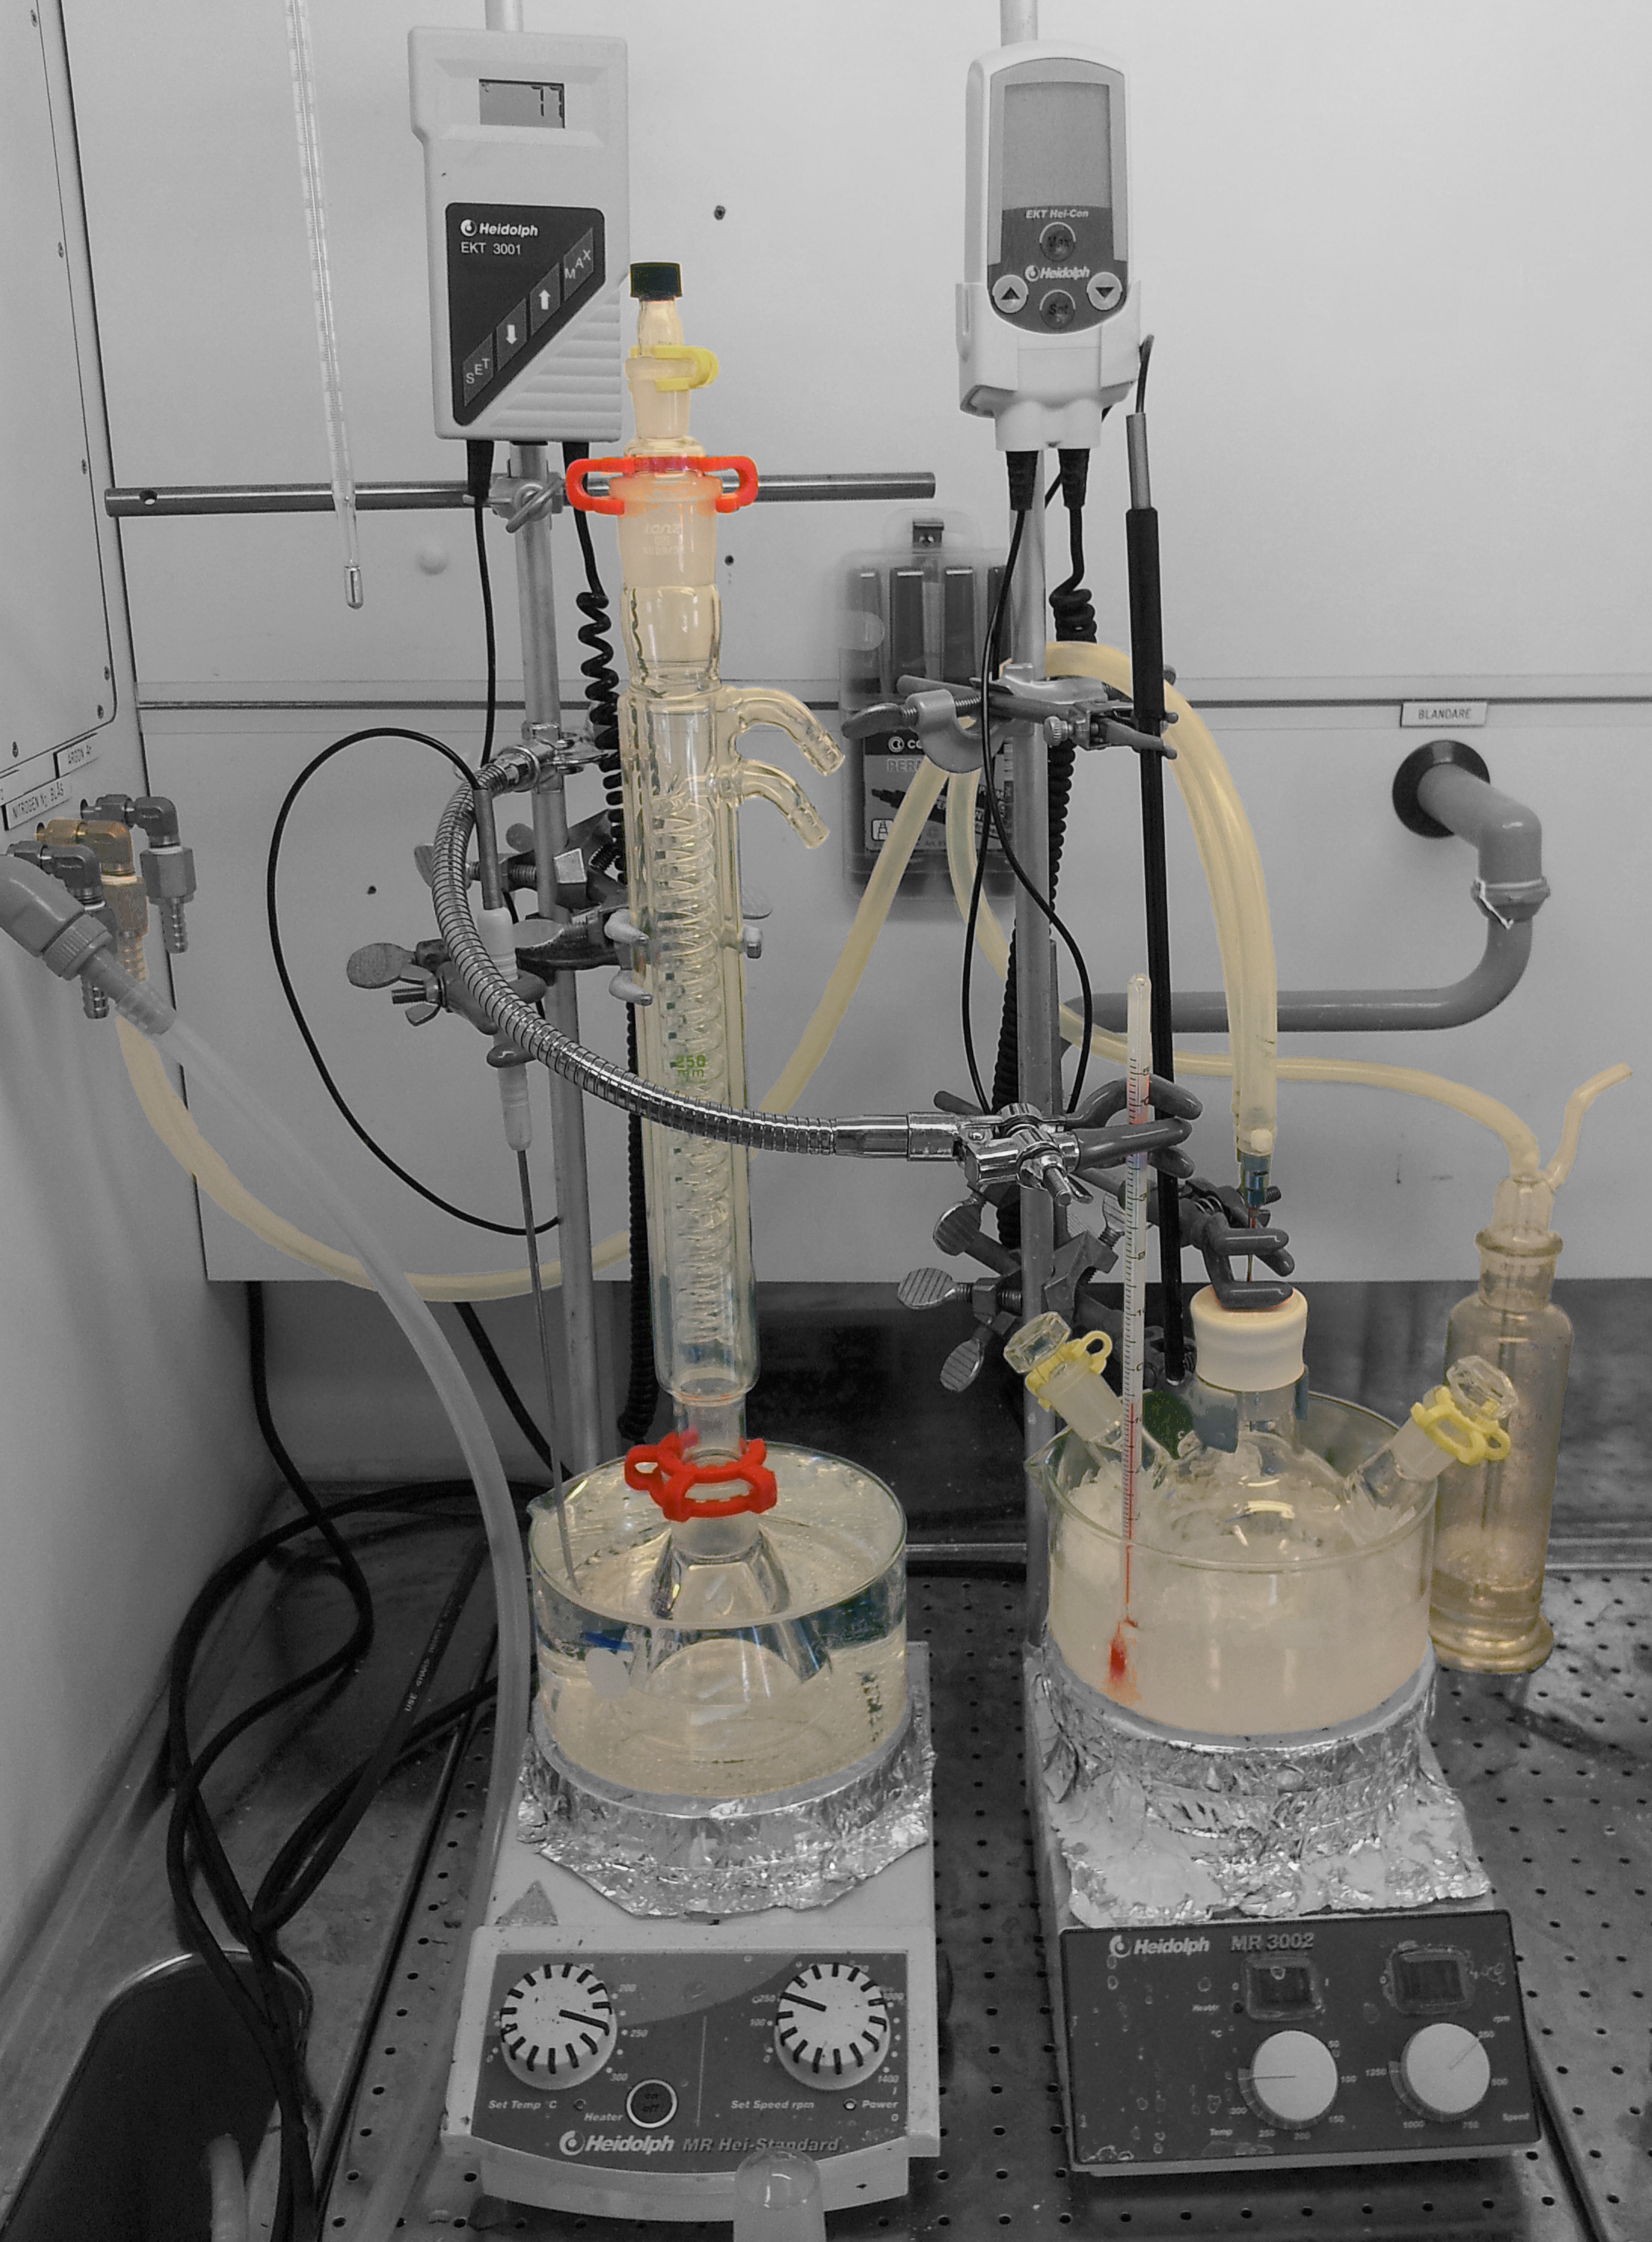
\includegraphics[width=0.40\textwidth]{synthesis/ZnO-QDs/ZnO-QD-synthesis-setup-bw-background-cropped}};
   % for this photo I have used both selective colourisation (I created an overlaying BW layer and selectively
   % decolourised it, giving the effect where the colourised objects appear to pop against the grayscale
   % background.
   % Because the fume hood lighting is very yellow, I have also adjusted hue-saturation
   % (decreasing yellow saturation and increasing lightness).
% create coordinate system relative to image size
\begin{scope}[x={(image.south east)},y={(image.north west)}, inner sep=1pt, thick]
   % \draw[help lines, xstep=0.1, ystep=0.1] (0,0) grid (1, 1);
   % identify coordinates of components
   \node (zincacetate) at (0.42,0.07) [rectangle] {};
   \node (lithiumhydrox) at (0.79,0.08) [rectangle] {};
   % labels
   % https://tex.stackexchange.com/questions/42401/transparent-node-with-opaque-text
   \node[fill=white,opacity=0.5,text opacity=1,outer sep=5pt,scale=1.8] at (zincacetate) {\reactant*[switch=true]{zincacetatedihydrate}};
   \node[fill=white,opacity=0.5,text opacity=1,outer sep=5pt,scale=1.8] at (lithiumhydrox) {\reactant*[switch=true]{lithiumhydroxidehydrate}};
\end{scope}
\end{tikzpicture}
\caption[ZnO QD synthesis setup]{%
   Our setup for the synthesis of \ch{ZnO} \protect\glsplural{QD}, allowing
   the simultaneous synthesis of the two precursor solutions.
   On the left, boiling \reactant[solvent=\EtOH,concentration=0.10]{zincacetatedihydrate}
   under open atmosphere with water-cooled refluxer, and on the right
   \reactant[solvent=\EtOH,concentration=0.14]{lithiumhydroxidehydrate} dissolved at
   \qty{45}{\celsius} in a sealed reactor under \ch{N2\gas} over-pressure.
   The glassware and gas flow components have been artificially highlighted in the photo.
}
\label{fig:0204-synthesis-QD}
\end{SCfigure}

Preparation of precursor solutions was as follows:
\begin{itemize}[after=\vspace{\baselineskip}]
\item add approximately \solvent[volume=45]{ethanol} to the Zn-reactor (\qty{100}{\mL} Erlenmeyer flask)
      and a magnetic stirrer bar; set temperature of water bath to boiling point of \solvent{ethanol},
\item turn on \ch{N2\gas} flow into the empty Li-reactor (round bottom flask) for a few minutes
      to purge \ch{CO2\gas} from it; add a magnetic stirrer bar;
      set temperature of water bath to \qty{45}{\celsius},
\item quantitatively transfer the weighed mass of \reactant{zincacetatedihydrate} to the boiling \solvent{ethanol},
\item add approximately \solvent[volume=50]{ethanol} and quantitatively transfer the weighed mass
      of \reactant{lithiumhydroxidehydrate} to the round-bottom flask,
\item once the mixtures have dissolved and the solutions
      are transparent and colourless move both reactors to an ice bath,
\item quantitatively mix the two precursor solutions to \qty{100}{\mL}
      (fill to the mark with \solvent{ethanol} as needed). Stir.
      Note the time ($t=\qty{0}{\minute}$ for \gls{QD} growth).
\end{itemize}

Both salts were easy to handle, weigh up and transfer.
The zinc acetate \reactant*[switch=true]{zincacetatedihydrate} dissolved easily after
a few minutes stirring in boiling \reactant{ethanol}.
But this solution was not stable for long: after a few hours it formed a milk-white suspension.

The lithium hydroxide \reactant*[switch=true]{lithiumhydroxidehydrate} has a more
challenging chemistry, primarily due to its carbonate salt.
Whereas both the dry and the slaked hydroxide have moderate solubility in \water\ and \EtOH,
with increasing solubility with increasing temperature, the
lithium carbonate, on the other hand, has poor solubility in \water\ and \EtOH,
and its solubility \emph{decreases} with increasing temperature.%
\footnote{%
   The solubility of \ch{Li2CO3} in water is \qty{1.54}{\gram} at \qty{0}{\celsius},
   and \qty{1.33}{\gram} at \qty{25}{\celsius} \cite{CRC104}.
   This points to an entropy effect, \ie, the solvation of \ch{Li+} and \ch{CO3^{2-}}
   in water decreases the overall entropy of the solution.}
In practice, this meant that during dissolution of
\reactant[solvent=\EtOH,concentration=0.14]{lithiumhydroxidehydrate} we needed
to take care to limit the competing dissolution reaction of \ch{Li2CO3}, which was
driven by the presence of dissolved \ch{CO2}.
Since the hydroxide is only moderately soluble to start with, we needed to use
as large a volume of solvent as possible. To avoid encouraging the formation
of the carbonate, \ch{CO2\gas} should be kept out of the headspace, and in addition
one should avoid heating the solution (definitely not boil it) so as not decrease
the solubility of any lithium carbonate that may form.
In short, the higher the temperature and the higher the flow rate of \ch{N2\gas},
the more lithium ions were lost as insoluble carbonate, and
the more solvent was lost to evaporation, which were both detrimental to our process.

For the same reason, the lithium hydroxide solution \reactant*[switch=true]{lithiumhydroxidehydrate} must be stirred only gently.
Even moderate stirring will draw in more air (which even under \ch{N2\gas} flow may contain
\ch{CO2\gas}) into the solution, making it easier to form \ch{Li2CO3}.
This reaction also neutralizes at least one hydroxide ion, thus decreasing the
precursor solution's apparent \pH.
Of course, strictly speaking \pH\ is not defined in a non-aqueous solvent,
but we may still use it as a proxy to discuss the changing chemistry of \EtOH\ as
air (containing \carbondiox) equilibrates with it.
To investigate this, I measured the proton activity (apparent \pH) of \EtOH\ of
two different purities using a regular \pH-meter,
and found \pH{\,\num{8.35}} (\qty{99.5}{\percent}) and \pH{\,\num{8.19}} (\qty{99.96}{\percent})
immediately after opening the factory-sealed bottle;
and \pH{\,\num{7.83}} and \pH{\,\num{7.40}} after aerating the samples overnight.
These observations suggest that equilibration with air, just like for \water, significantly
alter the carbonate chemistry of the solvent, which may influence the \gls{QD} synthesis,
and that varying trace amounts of \water\ in \EtOH\ were likely not decisive.
All \ZnO\ \gls{QD} in this work were synthesized using \solvent[purity=99.5]{ethanol}
for reasons of cost, and used more or less immediately after opening the bottle.%
\footnote{%
   With the benefit of hindsight, I should perhaps have let the \solvent{ethanol}
   solvent aerate fully (until the \pH{} settled) before preparing the precursors.
   This did not effect the quality of individual batches, but may have improved
   repeatability between batches.}

To prepare precursor solutions at precisely the intended concentration it is important to
maintain the desired solvent volume, which was challenging since \solvent{ethanol} evaporated
so readily, especially when boiling.
Instead of sealing the glassware (which changes the boiling point of the solvent)
we fitted the \ch{Li}-reactor with a water-cooled reflux tube which successfully captured
and returned effectively all the evaporated solvent.





%%% CHAPTER:
%%% CHARACTERISATION METHODS
\chapter{Characterization methods}%
\label{ch:characterization-methods}


%%% SECTION
\section{UV-Vis spectroscopy}
\label{methods:uvvis-spectroscopy}

An object under irradiation can interact with the light in various ways.
From an optical perspective, the incident light has to penetrate the surface of
the object to interact with the material in the bulk of the object. And then the
light has to penetrate another surface to exit the object \cite[p.\,71]{Stenzel2005}.

For light incident on an object, the light may
\begin{enumerate*}[label=(\alph*)]
\item be transmitted through the object (in a well-defined direction),
\item be diffusely scattered at the object interfaces or in its interior,
\item be specularly reflected, or
\item be absorbed at the object interfaces or in its interior.
\end{enumerate*}
If we posit that these processes are the only interactions that can occur
between the incident light and the object, then conservation of energy requires:
\begin{equation}\label{eq:TRSA=1}
\glsname{transmittance} + \glsname{reflectance} + \glsname{scattering} + \glsname{absorbance} = 1
\end{equation}
where \glsname{transmittance} is the \glstext{transmittance},
\glsname{reflectance} is the \glsdisp{reflectance}{specular reflectance},
\glsname{scattering} is the \glsdisp{scattering}{diffuse scattering}, and
\glsname{absorbance} is the \glstext{absorbance}.

The \glstext{transmittance} is also related to the \glstext{absorption_coefficient}
and the path length, $L$ in the familiar Beer-Lambert law
(also illustrated in the margin):
\begin{equation}\label{eq:transmittance}
\glsname{transmittance} \equiv \frac{I}{I_0} = \exp(-\glsname{absorption_coefficient}L)
\end{equation}

In most of my work, we were mainly interested in the optical absorption.
\marginpar{%
%\input{assets/aux/fig/fig_0301-beer_lambert_law.Rnw}

%%%%%%%%%%%%%%
% PARAMETERS %
%%%%%%%%%%%%%%
\definecolor{LBParticlesColor}{RGB}{193,154,107} % Particles color
\def\cols{15}                        % Number of columns
\def\rows{30}                        % Number of rows
\def\SquareUnit{.25}                 % Lengths of unit square edges (cm)
\pgfmathsetmacro\RmaxParticle{.1}    % Maximum particle radius
\def\BeforeLight{3}                  % Light path before particle cloud

\begin{tikzpicture}[%
   scale = 0.75,%
   font=\scriptsize,%
   x = \SquareUnit cm,%
   y = \SquareUnit cm,%
   line width = 1pt]

%%%%%%%%%%%%%%
% LIGHT PATH %
%%%%%%%%%%%%%%
%-> Before particles cloud
\draw[%
   red,
   decoration = {markings, mark = at position 0.8 with {\arrow[]{latex}}},
   postaction = {decorate}] %
   (-\BeforeLight,{\rows*\SquareUnit/2})--++(\BeforeLight,0) node[midway, above, black]{$I_0$};

%-> Trespassing particles cloud
\draw[%
   decoration = {color change, start color = red, end color = red!20!white},
   decorate] (0,{\rows*\SquareUnit/2})--++(\cols*\SquareUnit,0);

%-> After particles cloud
\draw[%
   red!20!white,
   decoration = {markings, mark = at position 0.8 with {\arrow[]{latex}}},
   postaction = {decorate}] %
   ({\cols*\SquareUnit},{\rows*\SquareUnit/2})--++
   (\BeforeLight,0) node[midway, above, black]{$I$};

%%%%%%%%%%%%%%%%%%%
% PARTICLES CLOUD %
%%%%%%%%%%%%%%%%%%%
%-> Lua version (FASTER)
\foreach \i in {1,...,\cols}{
   \foreach \j in {1,...,\rows}{
      \edef\radius{\pr{\RmaxParticle*math.random()}}
      \edef\l{\pr{\SquareUnit-2*\radius}}
      \edef\x{\pr{(\i-1)*\SquareUnit+\radius+\l*math.random()}}
      \edef\y{\pr{(\j-1)*\SquareUnit+\radius+\l*math.random()}}
      \fill[LBParticlesColor] (\x,\y) circle[radius=\radius];
   }
}

%-> pgfmath version (uncomment it if you want to try)
% Some time compilation gives too high number computation problem
% \foreach \i in {1,...,\cols}{
% 	\foreach \j in {1,...,\rows}{
%       \pgfmathsetmacro\radius{\RmaxParticle*\rnd}
%       \pgfmathsetmacro\l{\SquareUnit-2*\radius}
%       \pgfmathsetmacro\x{(\i-1)*\SquareUnit+\radius+\l*\rnd}
%       \pgfmathsetmacro\y{(\j-1)*\SquareUnit+\radius+\l*\rnd}
%       \fill[LBParticlesColor] (\x,\y) circle[radius=\radius];
%    }
% }

%%%%%%%%%%%%%%%%%%
% LENGTH QUOTING %
%%%%%%%%%%%%%%%%%%
\draw[|<->|, > = latex, line width = .8pt,black] %
   ($(0,\rows*\SquareUnit)+(0,1)$)--++
   (\cols*\SquareUnit,0) node[midway, above]{$L$};

\end{tikzpicture}
}
If scattering can be neglected, \cref{eq:TRSA=1} simplifies to
\begin{equation}
\glsname{absorbance} = 1  - \glsname{transmittance} - \glsname{reflectance}
\end{equation}
or in terms of incident and transmitted light
\begin{equation}
\glsname{absorbance} =
\log\left(\frac{I_0}{I}\right) =
-\log(\glsname{transmittance})
\end{equation}
In practice, \gls{absorbance} is the base-10 logarithm of the spectral radiant power
transmitted through a reference sample divided by that
transmitted through the investigated sample, both observed in identical cells.

Note that \emph{absorptance}, defined as $-\log(1-\frac{I_\text{abs}}{I_0})$ \cite{Cohen2008}
is sometimes used in lieu of \glsname{absorbance} for samples where scattering
is not negligible, is algebraically equivalent to \glsname{absorbance}, since
$I_\mathrm{abs} = I_0 - I$, and thus the expression above can be rearranged
to $\log\left(\frac{I_0}{I}\right)$.

The \glstext{absorbance} can thus be determined by measuring both the \glstext{transmittance}
and the \glstext{reflectance} of a sample. Or, if reflectance can be neglected, then simply
by measuring its transmittance.

For a thin film, the amplitude and intensity of reflected or transmitted beams
of light can in principle be determined by setting up Maxwell's equations
and applying the appropriate boundary conditions \cite{Heavens1955}.
In practice that is very cumbersome and not something often done.
More to the point, for a thin film the \glstext{absorbance} equals the
\glstext{absorption_coefficient} times the film thickness, $d$: $A=\alpha d$.
The \glstext{absorption_coefficient} of a thin film can be expressed in terms
of the reflectance and transmittance \cite{Green2012}:
\begin{equation}\label{eq:alpha-thickness}
\glsname{absorption_coefficient} = \frac{1}{d}\ln\left(\frac{1-R}{T}\right).
\end{equation}
And if the thickness, $d$, is not known, simply rearrange the equation so the
left-hand side gives you $\glsname{absorption_coefficient}d = \glsname{absorbance}$.


We have employed \gls{UV-Vis-NIR} spectroscopy extensively, and with a few
different instruments.
For \insitu\ experiments on films or colloidal suspensions I used an
OceanOptics HR2000+ high-resolution fibre-optic spectrometer,
with a Mikropack DH-2000-BAL \gls{UV-Vis-NIR} light source using
both a deuterium lamp and a halogen lamp.
This setup was controlled \via\ a computer running SpectraSuite on Microsoft Windows~XP.
\Exsitu\ experiments on films were measured on the venerable PerkinElmer Lambda~900
\gls{UV-Vis-NIR} spectrophotometer equipped with an integrating sphere
(\eg, \cref{P1}, \cref{fig:P01-uvvisir-absorbance}).

\Gls{UV-Vis-NIR} spectroscopy gave us optical transmittance, reflectance, and/or absorbance
for both thin film and colloidal samples, which allowed me to track semiconductor band edges
and dye absorption peaks, among other features.



%%%% SECTION
\section{Photoluminescence spectroscopy}
\label{methods:photolum}

In \glsfirst{PL} spectroscopy the sample is excited with photons with higher
energy than its band gap and the sample's emission spectrum is recorded \cite{Pazoki2020},
\ie, photons in and photons out.
I have used \gls{PL} to study surface or interface phenomena involving
the absorption of photons that generate electron-hole pairs, which is of central
importance in \glstext{PC} \cite{Kundu2011a}.

In \gls{UV-Vis} fluorospectrometry (also known as \glsfirst{PL} spectrometry)
the sample under study is placed in front of a light source with a suitable bandpass filter
between them so that only a particular wavelength in the \gls{UV-Vis} region illuminates the sample.
Since the sample's emission can be assumed to be isotropic, the direction of excitation was set at
an angle to the detector to avoid detecting the incident light.
Special care was taken to keep stray light out of the spectrometer
(the room was darkened and the instrument was covered).

I recorded fluorescence spectra of electrodeposited \ch{ZnO} \glsplural{NR} on
\gls{TCO}-glass with and without \gls{CBD} \ch{CdS}.
Room-temperature steady-state emission spectra were recorded on a Fluorolog~3%
\footnote{%
   The Fluorolog 3's control software was based on the Origin~Pro software suite,
   with all recorded data saved as Origin plots by default. Not very convenient
   if you are not an Origin user.
   Using Origin's built-in command prompt, the data could be exported to ASCII
   in a two-liner: \texttt{fdlog.openpath(); }%
   % verb in footnote required fancyvrb package
   % https://tex.stackexchange.com/questions/203/how-to-obtain-verbatim-text-in-a-footnote
   \verb+{doc -e W {save -w %H %B%H.txt}}+%
   .%
}
(Horiba Jobin Yvon)
equipped with double-grating excitation and emission monochromators and a
\qty{450}{\watt} \ch{Xe}-lamp.
The main sample series (\ch{CdS}-coated \ch{ZnO} \glsplural{NR} on \gls{TCO}-glass)
was measured using right-angle (RA) detection with the sample substrate at \ang{30}
and always with the EE (electrode--electrolyte) surface facing the incident beam,
in order to minimize inner-filter effects.
The excitation and emission slits were set to obtain \qtylist{2;3;6}{\nm} and
\qtylist{4;6;8}{\nm} band passes, respectively (depending on excitation wavelength).
Integration time was set to \qty{0.1}{\second} per point.
A \qty{400}{\nm} long-pass filter was placed \emph{after} the sample to reduce
second-order diffraction by the excitation monochromator
(for $\glsname{wavelength}_\text{\glsname{excitation}}=\qty{350}{\nm}$ and \qty{375}{\nm}).
The emission spectra were corrected for the spectral sensitivity of the
detection system by using a calibration file of the detector response.





%%%% SECTION
\section{Raman spectroscopy}
\label{methods:raman-spectroscopy}

As we previously discussed (\cref{methods:uvvis-spectroscopy}), light interacts
with matter in a variety of ways.
When incident light is scattered by an object, it is overwhelmingly likely to
be \emph{elastically} scattered, meaning the light is propagated without changing
its wavelength (or equivalently, its energy or frequency).
With Raman spectroscopy we measure the \emph{inelastic} spectrum scattered from the
sample under illumination by laser light (high-power density, coherent, monochromatic, collimated light).
In this process the vast majority of the incident laser light is scattered
\emph{elastically} (Rayleigh scattering), and only about one inelastic scattering event
occurs for every \num[retain-unity-mantissa=false]{1e7} elastic scattering events (\qty{0.1}{\ppm}).
The inelastically scattered light has a very slightly different wavelength than the incident light,
because it has exchanged vibrational (or rotational) quanta with the specimen, which
can only occur if the polarizability of the specimen's electron cloud is changing
during the vibration \cite{Rahman2020a}, and thus carries with it information on the vibrational state
of the specimen which is correlated to its chemical bonding, chemical composition,
and phases in crystalline materials.

For some crystal structures, Raman and \gls{IR} are complementary, in the sense
that the crystal's vibrational modes are either Raman \emph{or} \gls{IR} active.
A lattice vibration can be simultaneously Raman and \gls{IR}-active only in
non-centrosymmetric crystal structures (\eg, polar crystals such as \ZnO,
\cf\ \cref{tab:0300-pxrd-pdfs}).
All molecules and solids have vibrational spectra, and nearly all vibrations
are either Raman or \gls{IR} active \cite{Dyer2005}.

Inelastic scattering of light by matter was first theorized by \textcite{Smekal1923} and
shortly after by \textcite{Kramers1924,Kramers1924a,Kramers1925}. This was around
the same time as Venkata Raman was pondering the molecular diffraction of deep bodies
of seawater during a voyage across the Indian Ocean \cite{Raman1922},
which led him and Krishnan to experimentally describe the Raman effect a few years later
\cite{Raman1928,Raman1928a}. The Raman effect was also independently described
experimentally in the USSR by Landsberg \& Mandelstam \cite{Landsberg1928,Landsberg1928a}.
The earliest investigations of the Raman effect in semiconductors occurred after
the advent of the laser in the 1960s \cite{Cardona1974}.

The terminology we use to assign vibrational spectral modes was determined
by an ICSU Joint Commission for Spectroscopy in 1953 \cite{Cohen2008} but is
commonly referred to as \textcite{Mulliken1930,Mulliken1955,Mulliken1956} notation.

In this thesis we concern ourselves with the Raman effect in crystalline semiconductors.
Semiconductors always have more than one atom in their unit cell, which leads
the dispersion relations (the relationship between frequency and wave vector) to
always exhibit two kinds of phonons with which photons can interact, \namely,
the \emph{optical} and \emph{acoustic} modes of lattice vibration.
The interaction with optical phonons%
\footnote{
   They are called \emph{optical} phonons because they can be
   excited by electromagnetic radiation in the optical wavelength region.
}
is what typically generates Raman scattering, and
the interaction with acoustic phonons results in so called Brillouin scattering
(first predicted by \textcite{Brillouin1922} in 1922) \cite{Pankove1975}.
Both optical and acoustic phonons have longitudinal and transverse modes,
depending on whether the vibration is along the direction of propagation
or orthogonal to it.

An incident photon of a certain wavelength can give or gain some of its energy
to the lattice in the form of a phonon.
The precise amount of energy gained or lost by the lattice is compensated by
an increase (Stokes) or decrease (anti-Stokes) in the wavelength (energy) of
the scattered light \cite{Loudon1964,Pankove1975}.
A phonon is a many-body-type quasiparticle;%
\footnote{%
   Some other commonly encountered quasiparticles are
   \textbf{polaritons} (coupled photon--optical phonon modes),
   \textbf{excitons} (an electron--hole pair),
   \textbf{polarons} (coupled electron--phonon modes),
   \textbf{plasmons} (a collective excitation of all the electrons in the crystal, \ie, a quantum of plasma oscillation),
   \textbf{magnons} (a collective spin excitation of the lattice),
   and
   \textbf{trions} (a localized excitation of two holes and one electron or two electrons
   and one hole that may occur in optically excited semiconductor nanostructures).}
a quantized lattice vibration and describes a collective motion of atoms in the lattice.
Phonons play an important role in determining a material's thermal, optoelectronic,
and electrical transport characteristics \cite{Senga2019}.
At $\glsname{absolute_temperature}=\qty{0}{\kelvin}$, a crystal lattice would contain no phonons.
At any temperature above absolute zero all matter vibrates to some extent,
due to lattice vibrations being quantized.
A material's phonon structure is fundamentally related to its thermodynamic
properties.

%\input{assets/aux/fig/fig_3300-vibrational-energy-levels.Rnw}

\begin{figure}[tbp]
\centering
\includegraphics[width=0.90\textwidth]{Raman-IR-Rayleigh-energy-levels.jpg}
\caption[Rayleigh, Raman and IR scattering]{%
   Rayleigh, \protect\gls{IR}, and Raman (Stokes, anti-Stokes, and resonance) scattering.
   Resonance Raman scattering occurs when the excitation energy coincides with
   an electronic transition (such as the band gap) in the material.
   Illustration courtesy of \textcite{Qiu2019}.
}
\label{fig:0300-vibrational-energy-levels}
\end{figure}

Another way to look at this interaction is that the incident photon excites a phonon,
causing the semiconductor to re-emit the remaining (or gained) energy as a photon.
This scattering process is generally isotropic, which is why Raman scattering is
commonly measured in the antiparallel direction to the incident beam. Also, both
the incident and emitted light typically have limited penetration depth in the sample,
which also restricts detection to the reflection direction
(just like for \gls{SEM} and many other techniques with opaque samples).

The created phonon can in turn interact with the lattice to produce a second phonon
(of lower energy than the first), and this cascade process can be repeated,
generating what is called second-, third-, fourth-order (and so on) Raman scattering,
or more generally termed \emph{multiphonon} scattering.
Note that if the energy of the phonon coincides with the energy of an exciton (\emph{resonance}),
the intensity of the higher-order phonon can be strongly enhanced \cite{Pankove1975}.

In polar semiconductors, \ie, materials with a permanent electric polarization
due to the relative displacement of positive and negative ions in the crystal
structure (in other words, ionic crystals), with few defects
interaction between this polar electric field and
the optical phonons is expected to be the dominant scattering mechanism at \gls{RT}.
This so called polar--optical-phonon scattering interacts with the charge carriers
in what is known as the Fröhlich interaction \cite[p.\,40]{Stroscio2005}.

This interaction of optical phonons and charge carriers in polar semiconductors
in many cases determines its carrier mobility \cite{Stroscio2005}
\enquote{The carrier mobility in the presence of an external electric field is determined
predominantly by the rate at which the electrons emit optical phonons} \cite{Stroscio2005}.

Raman spectroscopy is non-destructive, simple, and often (but not always) a quick method
to determine which crystal phases are present in a solid or solute sample.
It yields information about bonds and crystallinity, and we can use it to tell apart
different polymorphs of the same composition (\eg, \glsxtrlong{hematite} from maghemite)
which is not always straight-forward with \gls{XRD}.
One of the major weaknesses of Raman spectroscopy is fluorescence from a sample,
which can completely swamp the inelastically scattered signal and be very hard
to overcome.



\subsection{Resonant Raman scattering}
\label{methods:resonant-Raman}

As we have seen, regular phonon scattering (\ie, non-resonant) occurs through
excitation to virtual intermediate electronic transitions.
In this section we will briefly describe \emph{resonant} Raman scattering by optical phonons
as utilized in \cref{P4}.

When the wavelength (\ie, energy or frequency) of the incident light approaches one
of the electronic transitions of the crystal (such as the band gap in a semiconductor),
the Raman scattering can be enhanced by many orders of magnitude (this effect
was first reported in crystals by \textcite{Ovander1962}).
Achieving resonance used to be hard because the wavelength of the incident
laser light must be close to the band gap under study, and it is only with the
development of high-power \gls{UV} laser sources
that wide gap semiconductors such as \ZnO\ came within reach of resonance studies.
But even with the intensity gained from resonance, resonant Raman experiments
may be saddled with an even stronger phonon-aided luminescence that can drown out
all or some of the Raman modes, which is a drawback particularly affecting samples
with any organic residues (even very small amounts).

Under electronically exciting conditions (\ie, resonance) Raman can provide
information on vibrations in the excited state and can also give clues towards
the charge separation/transfer mechanisms in the material \cite{Rahman2020a}.
Polar crystals often complicate resonance by
leading to the introduction of multiphonon processes caused by
intraband Fröhlich interaction \cite{Cardona1983}.

%\input{assets/aux/fig/fig_0303-raman-setup.Rnw}

\begin{figure}[tbp]
\centering
\begin{tikzpicture}
   \node (mainphoto) at (0,0) {\includegraphics[width=0.75\linewidth]{methods/raman/powder-samples-measurement}};
   % inset in lower left corner
   \node[anchor=south west,xshift=-3mm,yshift=-3mm,draw=white,line width=1.5mm,inner sep=0pt] (wellplate) at (mainphoto.south west) {\includegraphics[width=0.33\linewidth]{methods/raman/liquid-precursor-measurement}};
\end{tikzpicture}
\caption%
[A Raman measurement]{%
   Photo by the author of a particularly organised series of Raman measurements on \zincox{}
   powder samples (\cref{P4}), showing the objective lens mount of the Ramanoscope and its sample tray.
   The inset shows a close-up of the transparent sample wells on the tray.
}
\label{fig:0403-raman-setup}
\end{figure}

A challenge when using resonant Raman for wide gap materials
is the need to utilize \gls{UV} light, which puts added constraints on the
optical components in the Raman spectrometer, which is why
we used a near-UV objective and \gls{UV} lenses in the spectrometer's
optical path. All measurements were recorded at ambient conditions.
Resonant Raman was measured with the \qty{325}{\nm} excitation line of a \ch{He}-\ch{Cd} laser,
using a 15x/0.30 NUV objective lens (Thorlabs).
The detector was calibrated against the \qty{1332}{\per\cm} line of diamond.
All measurements in the resonant experiment series used the exact same acquisition
parameters.
Cosmic rays were removed either by the detection and removal algorithm
built-in to the Renishaw software suite, or manually at a later stage by
linear interpolation over the affected data points.
Peak and baseline fitting was performed with the algorithm by \textcite{Davies2008}
(also see \cref{method-development:spectral-peak-fitting}).




%%%% SECTION
\section{Photocatalysis}
\label{methods:photocatalysis}

In order to evaluate the \glsdisp{PC}{photocatalytic} or
\glsdisp{PEC}{photoelectrochemical} properties of the
catalysts we synthesized, we employed both solar simulators
(emulating the standard \gls{AM15G} spectrum to varying degrees of fidelity)
and custom or off-the-shelf lamps.
I designed and built many of the experimental setups from scratch.


\subsection{The solar spectrum}
\label{pc:solar-spectrum}

To get a firm grasp of the solar spectrum it helps to first
understand the black body spectrum and the concept of \gls{AM}.

The \glstext{spectral_radiance} of an ideal black body%
\footnote{%
   Every object at above \qty{0}{\kelvin} emits and absorbs electromagnetic
   radiation to some degree. An object that absorbs all radiation is a black body
   and by definition has an emissivity of unity. For a black body the
   spectral distribution of this radiation depends \emph{only} on the object's
   \glstext{absolute_temperature}.}
is given by Planck's law%
\footnote{%
   By the year 1900, physicists had been trying to understand the dependence of the black body spectrum
   as a function of temperature and wavelength for almost half a century.
   Several proposed equations existed, but as they were within the confines of
   classical physics they all failed to match observations at higher frequencies.
   As the story is commonly told, in an act of desperation (Planck feared being scooped)
   he submitted an equation that seemingly worked but made use of Boltzmann's entropy law which
   rested on the assumption of atoms (quanta) and was statistical,
   both phenomena disliked by Planck who was a conservative physicist.
}
\cite[sec.\,2.3]{Suppan1994}
\begin{equation}\label{eq:planck}
\glsname{spectral_radiance} =
   \frac{2{\pi}\glsname{Planck_constant}\glsname{speed_of_light}^2}{\glsname{wavelength}^5}%
   \frac{1}{\exp\left(\displaystyle\frac{%
      \glsname{Planck_constant}\glsname{speed_of_light}}{%
      \glsname{wavelength}\glsname{Boltzmann_constant}\glsname{absolute_temperature}}%
   \right) - 1}
\end{equation}
This represents the emitted power per unit area of
emitting surface and per unit wavelength. \glsname{spectral_radiance} is called
the \glstext{spectral_radiance}, and when referring to a black body it is considered
independent of viewing angle (isotropic), independent of time, and independent of
position on the emitting surface (spatially homogeneous).

%\input{assets/aux/fig/fig_0101-blackbody-spectralradiance.Rnw}












%\input{assets/aux/tab/tab_0100-solarconstants.Rnw}

% latex table generated in R 4.1.3 by xtable 1.8-4 package
% Fri Dec 15 02:01:06 2023
\begin{table}[tbp]
\centering
\caption[Constants related to solar spectral irradiance]{Physical quantities related to Planck's law \cref{eq:planck} and the calculation of the solar spectrum. For sources please see \cref{photoec}.} 
\label{tab:0100-solarconstants}
\begin{tabular}{lcS[table-format=1.6e+2]l}
  \toprule
{Name} & {Symbol} & {Value} & {Unit} \\ 
  \midrule
Speed of light & \ensuremath{c} & 2.997925e+08 & \si{\metre\per\second} \\ 
  Elementary charge & \ensuremath{e} & 1.602177e-19 & \si{\coulomb} \\ 
  Planck's constant & \ensuremath{h} & 6.626070e-34 & \si{\joule\second} \\ 
  Planck's constant & \ensuremath{h_\text{eV}} & 4.135668e-15 & \si{\electronvolt\second} \\ 
  Boltzmann's constant & \ensuremath{k} & 1.380649e-23 & \si{\joule\per\kelvin} \\ 
  Temperature of the Sun & \ensuremath{T_\text{Sun}} & 5.772000e+03 & \si{\kelvin} \\ 
  Astronomical unit & \ensuremath{R_\text{AU}} & 1.495979e+11 & \si{\metre} \\ 
   \bottomrule
\end{tabular}
\end{table}


By plugging the surface temperature of the Sun (see \cref{tab:0100-solarconstants})
into \cref{eq:planck} we can accurately model its radiance and the irradiance on Earth%
\footnote{%
   For an \emph{emitting} surface, the term is \textbf{radiance},
   and for an \emph{absorbing} surface it is \textbf{irradiance}.}
(stars are to a very good approximation black bodies).
Once the sunlight enters our atmosphere, though, things become much more messy,
and we are better off leaving analytical equations behind and embracing
international standards.
To understand the \glsdisp{AM15G}{standard solar spectrum}
we need to briefly familiarize ourselves with the \gls{AM} concept.

%\input{assets/aux/fig/fig_airmass.Rnw}

\begin{figure}[tbp]
\centering

% green seems suitable for the ground level
% https://en.wikipedia.org/wiki/Shades_of_green#Sea_green
\definecolor{amseagreen}{HTML}{2E8B57}
% https://en.wikipedia.org/wiki/Shades_of_blue#Uranian_blue
\definecolor{uranianblue}{HTML}{AFDBF5}
\tikzstyle{horizon} = [%
   % https://texample.net/tikz/examples/oblique-incidence
   postaction={draw,decorate,decoration={border,angle=-45,amplitude=0.3cm,segment length=1mm}}]

\begin{subfigure}[b]{0.48\linewidth}
\centering
\begin{tikzpicture}[inner sep=0pt, outer sep=0pt]

% atmosphere
\fill[draw=none, fill=uranianblue, opacity=0.10] (0, 0) rectangle +(5, 2.2);

% to get the exact same distance between two lines, let's define two identical rectangles
% then use clipping to hide their short ends
\begin{scope} % AM1
   % use clipping to hide short ends both at horizon and up top
   \clip (0, 0) rectangle (1.2, 2.95);
   \node[rectangle, draw=orange, thick, anchor=south west, minimum width=21pt, minimum height=3cm] (AM1) at (0.2, 0) {};
   \node[anchor=south,yshift=0.2cm,font=\sffamily\footnotesize] (labelAM1) at (AM1.south) {AM1};
\end{scope}

\begin{scope} % AM1.5
   % use clipping to only show the part of this rectangle above the horizon line
   \clip (0, 0) rectangle (5, 3);
   % tried to avoid rotating the text label by using "shape border rotate=-48.2" but had no effect, nothing was rotated
   \node[rectangle, draw=orange, thick, anchor=south west, rotate=-48.2, minimum width=21pt, minimum height=5.5cm] (AM15) at (1.18, 0) {};
   % by tying this label to the AM1 label they get exactly the same height, but x-position is eye-balled
   \node[anchor=west,xshift=0.82cm,font=\sffamily\footnotesize] at (labelAM1.east) {AM1.5};
\end{scope}

% airmass at latitude of Ångström laboratory
% airmass(59.83919)
% [1] 1.990332
\begin{scope} % AM1.99
   % use clipping to only show the part of this rectangle above the horizon line
   \clip (0, 0) rectangle (5, 3);
   % thanks to clipping height can be anything (as long as it's long enough to go past the clip limits), but height
   % also determines the placement of the $d$ distance label and arrows (to move label downwards use shorter height)
   \node[rectangle, draw=orange, thick, anchor=south west, rotate=-59.84, minimum width=21pt, minimum height=4.2cm] (AM199) at (2.60, 0) {};
   \node[anchor=west,xshift=2.48cm,font=\sffamily\footnotesize] at (labelAM1.east) {AM1.99};
\end{scope}

% to get the ground shadow effect, let's redraw the same rectangles, but filled, and
% clip out everything except a sliver along the horizon
\begin{scope}
   \clip (0, 0) rectangle (5, 2pt);
   \node[rectangle, fill=orange, opacity=0.33, draw=orange, thick, anchor=south west, minimum width=21pt, minimum height=3cm] (shadow0) at (0.2, 0) {};
   \node[rectangle, fill=orange, opacity=0.33, draw=orange, thick, anchor=south west, rotate=-48.2, minimum width=21pt, minimum height=5.5cm] (shadow15) at (1.18, 0) {};
   \node[rectangle, fill=orange, opacity=0.33, draw=orange, thick, anchor=south west, rotate=-59.84, minimum width=21pt, minimum height=5.5cm] (shadow199) at (2.60, 0) {};
\end{scope}

% horizon
\draw[amseagreen, line width=.5pt, horizon] (0, 0) -- (5, 0);

% putting a simple label denoting distance turned out to be trickier than I expected
% the opacity/text opacity approach worked fine, but only in the niche PDF viewer Sioyek
% I hope this verbose approach will have better compatibility
% first, print the label
\node[anchor=center,font=\scriptsize] (distanceAM1) at (AM1.center) {$d$};
\draw[->] (distanceAM1) -- (AM1.east); \draw[<-] (AM1.west) -- (distanceAM1);
\node[anchor=center,font=\scriptsize] (distanceAM15) at (AM15.center) {$d$};
\draw[->] (distanceAM15) -- (AM15.east); \draw[<-] (AM15.west) -- (distanceAM15);
% \node[anchor=center,font=\scriptsize] (distanceAM199) at ($ (AM199.center) - (AM199.south) $) {$d$};
% \draw[->] (distanceAM199) -- (AM199.east -| AM199.south east); \draw[<-] (AM199.west -| AM199.south west) -- (distanceAM199);
\node[anchor=center,font=\scriptsize] (distanceAM199) at (AM199.center) {$d$};
\draw[->] (distanceAM199) -- (AM199.east); \draw[<-] (AM199.west) -- (distanceAM199);

% % https://tex.stackexchange.com/a/263897/10824
% \begin{scope}[transparency group] %[on background layer]
%    % an arrow to denote distance between the two parallel rays
%    % opacity and text opacity combo works perfectly in Sioyek but not in Evince nor Okular
%    % https://tex.stackexchange.com/questions/321974/tikz-node-fill-which-is-opaque-to-entities-in-tikzpicture-but-transparent-to-ba
%    \draw[<->] (AM1.west) -- (AM1.east) node [midway,fill=uranianblue,opacity=0.10,text=black] {$d$};
%    \draw[<->] (AM15.west) -- (AM15.east) node [midway,fill=uranianblue,opacity=0.10,text=black] {$d$};
%    % \draw[<->] (AM15.west) -- (AM15.east);
% \end{scope}

% \node [draw=black, fill=uranianblue, opacity=0.10] at (AM1.center) {$d$};
\end{tikzpicture}
\caption{}
\label{fig:airmasses}
\end{subfigure}%
\begin{subfigure}[b]{0.48\linewidth}
\centering
\begin{tikzpicture}[inner sep=0pt, outer sep=0pt,font=\scriptsize]
% \draw[help lines,xstep=1,ystep=1] (-4,0) grid (4,2);

% atmosphere
\fill[draw=none, fill=uranianblue, opacity=0.10] (-2, 0) rectangle +(5, 2.2);

% AM1.5G label
% position was manually adjusted
\node[anchor=north west,xshift=3pt,yshift=-2pt,font=\sffamily\footnotesize] at (-2, 2.2) {AM1.5G};

% ground level, horizon
\draw[amseagreen, line width=.5pt, horizon] (-2,0) -- (3,0);

% zenith line
% xshift tries to place the zenith through the center of the absorber (depends on its length and angle)
% https://www.calculator.net/right-triangle-calculator.html?av=&alphav=37&alphaunit=d&bv=&betav=&betaunit=d&cv=1&hv=&areav=&perimeterv=&x=59&y=18
% sqrt(square(1) - square(c*sin(37)))
% outer sep puts some separation between the label and the zenith line
\node [xshift=-0.399cm,fill=white, outer sep=1mm] (zenith) at (0,3) {zenith};
% https://tikz.dev/tikz-coordinates#sec-13.3.1
\draw[->,line width=.5pt] (zenith |- 0,0) -- (zenith.south);

\begin{scope}
   \clip (-2,0) rectangle (3, 3);
   % sun rays at AM1.5, m = 1/cos z => z = 48.2 from the zenith line
   % attempted to specify angle from the point of intersection between the ground line
   % and the zenith line, but that always led to angles being off by ~10°, quite weird
   % \draw [orange, thick, yshift=0cm, xshift=0cm] (zenith |- 0,0) -- (48.2:2cm);
   \foreach \x in {7pt, 0pt, -7pt, -14pt, -21pt, -28pt, -35pt}
      \draw [{Kite[length=4pt,width=2pt,inset=1pt]}-, orange, thick, yshift=0cm, xshift=\x] (0:0cm) -- ({90-48.2}:4.5cm);
   % solar disk
   % xshift in order to center the disk on the bunch of rays (manually adjusted)
   % size is simply the smallest large enough to envelop the rays (manually adjusted)
   \node[circle, draw=none, fill=orange, xshift=-8pt, minimum size=14mm] (sundisk) at (3,3) {};
\end{scope}

% flat surface of the same area (length)
% yshift down so its top surface is flush with ground level (simply to make it overlap less with the tilted surface)
\fill[draw=black, fill=black!50, fill opacity=0.8] (0,0) rectangle +(-1.00, -0.16);
% \fill[draw=black, fill=black!33, line width=4pt, yshift=-2pt] (0:0cm) -- (180:1cm);

% tilted surface
% 180 - 37 = 143, 90 + 53 = 143
% \draw[black,dashed,line width=0.4pt] (0:0cm) -- (143:2cm);
% \fill[draw=black, fill=black!66, line width=4pt] (0:0cm) -- (143:1cm);
\fill[draw=black, fill=black!50, fill opacity=0.8, rotate around={53:(0,0)}] (0,0) rectangle +(0.16, 1.00);
% angle arc for tilted surface
% \draw (-0.799, 0) arc (180:143:0.602cm);
% (x coord, y coord) arc from 180° to 143° (37°) drawn using 2 cm long line
% \draw (-1.5, 0) arc (180:143:2.0cm);
% https://tex.stackexchange.com/questions/38763/how-to-place-a-node-in-the-middle-of-an-arc
\draw (-0.9cm,0cm) arc [start angle=180, end angle=143, radius=9mm] node (labeltiltangle) [midway, anchor=east, xshift=-1pt, yshift=4pt] {\ang{37}}; % {$\theta{=}\ang{37}$};
% \path (-0.799,0) ++ (45:0.20cm) node{\ang{37}};
% \node [anchor=east] at (-0.9, 0.35) {\ang{37}};

% surface normal
\draw [dashed, thick, opacity=0.35, yshift=0.5cm, xshift=-0.25cm] (0:0cm) -- ({90-37}:2cm);

% arc for zenith angle (zenith line to AM1.5 rays)
% 90 - 48.2 = 41.8
% https://tex.stackexchange.com/questions/432166/tikz-label-of-node-midway-perpendicular-to-the-node
\draw (-0.399cm, 2.0cm) arc [start angle=90, end angle=41.8, radius=17mm] node [midway, above, yshift=1pt, sloped] {\ang{48.2}}; % {$z{=}\ang{48.2}$};

% arc for solar altitude (ground level to AM1.5 rays)
% midway puts the label on top of the rays, makes it look crowded, manually adjusted pos to shift label along the curve
\draw (1.0cm, 0cm) arc [start angle=0, end angle=41.8, radius=12.8mm] node [pos=0.29, above, yshift=1pt, sloped] {\ang{41.8}};
\end{tikzpicture}
\caption{}
\label{fig:AM15G-tilt}
\end{subfigure}%
\caption[Illustration of the air mass concept]{%
   Illustration of the \protect\glsxtrlong{AM} concept.
   (\subref{fig:airmasses})
   Demonstrating the geometric projection effect of different air mass values.
   As the air mass increases, the projected area on the ground of an identical
   beam of light increases (diameter $d$ is the same for all cases).
   AM1.99 corresponds to Uppsala's latitude.
   (\subref{fig:AM15G-tilt})
   Geometry of the AM1.5G standard, here shown with a light beam incident also
   on a horizontal surface, illustrating how
   the surface tilted \ang{37} collects more light.
   The \emph{zenith angle} is \ang{48.2} for AM1.5G, which is
   complementary to the \emph{solar altitude} (angle from the horizon, \ang{41.8}).}
\label{fig:airmass}
\end{figure}

The \glsxtrlong{AM} concept (see \cref{fig:airmass}) offers a compact way to express
the influence of atmospheric absorption and scattering (both of which depend on
path length in the atmosphere, \ie, \glsxtrlong{AM}) on the terrestrial irradiance
for all latitudes except for the highest.
Just outside the atmosphere, the \glsxtrlong{AM} is zero at all latitudes.
On the equator with the sun at zenith, \glsxtrlong{AM} is unity.
Assuming zero altitude (sea level) and a homogeneous plane-parallel atmosphere
(\ie, one in which density is constant and Earth's curvature is ignored),
\seemore{\cref{photoec}}
\gls{AM} is the secant of the zenith angle in degrees, $z$:
\begin{equation}\label{eq:airmass}
\mathrm{\glsname{AM}} = \sec(z) = 1/\cos(z)
\end{equation}
This equation breaks down above \ang{75} latitude, which is a problem
for astronomers but perfectly fine for our purposes.%
\footnote{%
   Better models of the atmosphere \cite{Woolard1966} demonstrate that
   \glsxtrlong{AM} reaches at most around \num{38} for astronomical objects
   towards the horizon ($z=\ang{90}$).
}




\subsection{Photocatalysis rigs}
\label{pc:rigs}

I designed several rigs for photocatalytic testing over the course of my work.
Some were tailored towards thin film evaluation and others towards the
evaluation of colloidal photocatalysts, all at room temperature
(no active cooling of the \gls{PC} reactor).
Our light sources are described in \cref{box:light-sources}.

%\input{assets/aux/box/box_light-sources.Rnw}




\begin{infobox}[Laboratory light sources]
\label{box:light-sources}

To maintain a stable power density on the irradiated sample it is always
advisable to allow the light source sufficient time to warm up before starting
the measurement, in order for any filament to reach its working temperature,
or heat transfer across a sink to reach equilibrium, \etc.
If the light is not too bright nor too dim, the evenness of the produced patch
can easily be judged simply by looking at it.
Evenness can be improved considerably by adding suitable optics in the light path.
Light sources are commonly rated by their power draw, but this says
nothing about the intensity of the produced light nor its spectral
distribution.
It is therefore important to measure both the power density of the lamp
(which depends on the distance) and its spectral distribution.

In contrast to natural sunlight, we can tailor the spectral output of a lamp
to suit a particular application, \eg, a wide gap semiconductor might be
put under illumination of a \gls{UV} lamp. Since light is effectively a reactant
in a \gls{PC} reaction, this can significantly increase its throughput.

\begin{center}%
\begin{knitrout}\scriptsize
\definecolor{shadecolor}{rgb}{0.969, 0.969, 0.969}\color{fgcolor}

{\centering \includegraphics[width=3.80in]{figure/0407-fig-PC-light-sources-1} 

}


\end{knitrout}
% captionof inside BOX (as in this case) needs to use smaller font size to match the box font size
\captionsetup{font+=footnotesize}
% I tried font+=\smaller but throws error "Illegal parameter number in definition of \XKV@naa"
\captionof{figure}[Representative emission spectra of common light sources]{%
   Emission spectra of black light \gls{CFL} (digitized from manufacturer's
   datasheet) and a custom-order blue \gls{LED} array (experimentally recorded),
   a xenon arc solar simulator lamp (experimentally recorded),
   typical white \gls{LED} (digitized from manufacturer's datasheet),
   and mercury arc lamp (experimentally recorded).
}
\label{fig:box-pc-light-sources}
\end{center}

Philips PL-S BLB/2P \gls{CFL} black light
with a power draw of \qty{8.6}{\watt} and producing
\qty{1.65}{\watt} \glsdisp{UV}{UV-A}
centered at \qty{370}{\nm} and with less than \qty{0.2}{\percent} \glsdisp{UV}{UV-B},
according to the manufacturer's datasheet.
This kind of lamp has the form-factor of a consumer-grade \gls{CFL}, is cheap and
easy to source but produces very little visible light (hence the name).
But because the light source itself is about a decimetre long
and half as wide, the power density even very close to the lamp was very low,
which made it unsuitable for our \gls{PC} experiments.

Our blue \gls{LED} was a custom-made array with \num{49} surface-mounted blue
\glsplural{LED} with an integrated heatsink and fan (branded \enquote{Allray}).
Spectral output was centered at \qty{450}{\nm}
with \glsxtrshort{FWHM} of $\qty{20}{\nm}$ and a
power draw of \qty{50}{\watt}.
We measured power density at the distance of the sample (\cf\ \cref{{fig:0400-pc-blue-vertical-with-condensers}})
to \qty{34(4)}{\mW\per\square\cm}.

The Oriel Instruments Newport 67005 solar simulator
used a xenon arc filament and an \gls{AM15G} optical filter
to produce \qty{100}{\mW\per\square\cm} at the sample
(\hlink{https://solarchemist.se/2016/04/23/lamps-filters}{see blog for details}).

The bottom-left panel shows a typical white \gls{LED} emission spectrum,
here represented by a Perkin-Elmer ACULED™ with a colour temperature of \qty{6500}{\kelvin}.
This spectral distribution is typical for
\ch{GaN} (emitting at \qty{465}{\nm}) and
\ch{Ce^{3+}:YAG} (\ch{Ce}-doped yttrium aluminium garnet) acting as a phosphor
emitting a broader Stokes-shifted yellow light. This sort of white light suffers
from \enquote{blue overshoot} and a \enquote{cyan gap},
which new materials based on perovskite nanostructures aim to overcome \cite{Peng2023}.

The high-pressure mercury arc filament can sustain very high intensities
(commercially known as a \enquote{tanning lamp}). Here showing the emission of a
Philips HPA 400S high-pressure mercury lamp (\qty{400}{\watt}).
Apart from broad \gls{Vis} emission it also outputs lots of \glsdisp{UV}{UV-A}
and heat.
\end{infobox}

After a few not-so-successful lighting setups
involving white-light \glsplural{LED} and \enquote{black light}
\glsplural{CFL} (both turned out to be too low-intensity for any experiments),
we achieved our first working \gls{PC} reactor (\cref{fig:0400-pc-blue-beaker})
using a high-intensity blue-light \gls{LED} array.
%
The reactor for this lamp was simply a beaker wherein the sample was placed
face-up on a custom-machined acrylic platform so that a magnetic bar could
freely spin underneath it and stir the solution.
Progress monitoring was done by periodically transferring a sample
of the solution to a cuvette for \exsitu{} \gls{UV-Vis} spectrophotometry.
This setup was used in \cref{P1}.

We quickly evolved the setup to use a quartz cuvette to allow \insitu{} \gls{UV-Vis} tracking,
but with the down-side of no longer being able to stir the solution
(see \cref{fig:0400-pc-blue-vertical-with-condensers}).
We managed to improve the intensity and uniformity of the light from
the \gls{LED} array with the addition of an optical tube (containing a convex lens
with adjustable position along its length) and two aspheric condenser lenses
(Thorlabs ACL-5040, $d=\qty{50}{\mm}$, $f=\qty{40}{\mm}$) to the optical path,
producing a dense and even patch of light approximately \qty{2}{\cm} in diameter.
We chose to continue mounting the light source vertically because the quartz cuvette
only had two transparent sides.
This setup was in \cref{P2}, where we also experimented with a mercury arc lamp.

I also performed a number of \gls{PC} experiments with a mercury arc lamp
(as a \enquote{poor-man's} solar simulator), which resulted in quite
poor photocatalytic degradation, but some interesting morphological
changes of our core--shell nanorods reported in \cref{P2}.

With our third and fourth generation of the \gls{PC} reactor
(\cref{fig:0400-pc-solarsimulator-thinfilm,fig:0400-pc-solarsimulator-suspension})
we graduated to using a solar simulator with a xenon arc lamp.
The proximate cause for this setup was to have the light impinge directly onto a
thin-film photocatalyst that was lying on the bottom of the cuvette (facing up).
The ultimate cause was that the quartz cuvette had only two transparent sides,
which meant \insitu\ spectrophotometry would not have been possible with horizontal illumination.
The light from the solar lamp hit a mirror placed at a \ang{45} angle above the cuvette.
The dye degradation was tracked \insitu\ using our fibre-optic spectrophotometer.

%\input{assets/aux/fig/fig_0300-pc-rigs.Rnw}

\begin{figure}[tbp]\centering
%%% SUBFIGURE LEFT
\hspace{\stretch{1}}%
\begin{subfigure}[T]{0.32\textwidth}\centering
\begin{tikzpicture}[font=\sffamily\tiny]
   \node[anchor=south west,inner sep=0] (image) at (0,0) {\includegraphics[trim={20mm 22mm 0 10mm},clip,width=\textwidth]{methods/photocatalysis/0117}};
   % inset in bottom edge
   % note: I have manually adjusted yshift so that bottom of this subfig aligns with bottom of the center subfig
   \node[anchor=south,xshift=0mm,yshift=-14.45mm,draw=white,line width=1.5mm,inner sep=0pt] (inset) at (image.south) {\includegraphics[trim={240mm 0 200mm 0},clip,width=0.36\linewidth]{methods/photocatalysis/0305}};
   % create coordinate system relative to image size
   \begin{scope}[x={(image.south east)}, y={(image.north west)}, inner sep=1pt, thick]
      % \draw[help lines,xstep=.1,ystep=.1] (0,0) grid (1.2,1);
      % identify coordinates of components
      \node (fan)      at (0.50,0.92) [rectangle] {}; % [rectangle,draw=red] {};
      \node (sink)     at (0.50,0.74) [rectangle] {};
      \node (led)      at (0.50,0.56) [rectangle] {};
      \node (tube)     at (0.50,0.48) [rectangle] {}; % Aluminium tube
      \node (sample)   at (0.45,0.36) [rectangle] {}; % Thin-film sample (catalyst)
      \node (platform) at (0.55,0.32) [rectangle] {}; % Sample platform
      % labels
      \node[fill=white] (fanlabel) at (fan) {Fan};
      \node[fill=white] (sinklabel) at (sink) {Heatsink};
      \node[xshift=10mm,fill=white,anchor=north west] (ledlabel) at (led.south east) {LED array};
      \node[xshift=6.5mm,fill=white,anchor=north west] (tubelabel) at (tube.south east) {\ch{Al} tube \& lens};
      \node[xshift=-5mm,fill=white,anchor=north east] (samplelabel) at (sample.south west) {Catalyst};
      \node[xshift=5mm,fill=white,anchor=north west] (platformlabel) at (platform.south east) {Platform};
      % connecting arrows
      \draw [->,bend left=20,white] (ledlabel.west) to (led.north east);
      \draw [->,bend left=20,white] (tubelabel.west) to (tube.north east);
      \draw [->,bend right=10,white] (samplelabel.east) to (sample.north west);
      \draw [->,bend left=20,white] (platformlabel.west) to (platform.north east);
   \end{scope}
\end{tikzpicture}
\caption{}
\label{fig:0400-pc-blue-beaker}
\end{subfigure}%
\hspace{\stretch{1}}%
%%% SUBFIGURE CENTER
\begin{subfigure}[T]{0.32\textwidth}\centering
\begin{tikzpicture}[font=\sffamily\tiny]
   \node[anchor=south west,inner sep=0] (image) at (0,0) {\includegraphics[width=\linewidth]{methods/photocatalysis/0908182809-cropped.jpg}};
   % create coordinate system relative to image size
   \begin{scope}[x={(image.south east)},y={(image.north west)}, inner sep=1pt, thick]
      % \draw[help lines,xstep=0.05,ystep=0.05] (0,0) grid (1,0.4);
      % identify components with nodes
      \node (fan)  at (0.67,0.93) [rectangle] {}; % [rectangle,draw=red] {};
      \node (sink) at (0.67,0.84) [rectangle] {};
      \node (led)  at (0.67,0.77) [rectangle] {};
      \node (cyl)  at (0.67,0.65) [rectangle] {};
      \node (C1)   at (0.75,0.58) [rectangle] {};
      \node (C2)   at (0.75,0.43) [rectangle] {};
      \node (cuv)  at (0.71,0.16) [rectangle] {};
      % labels
      \node[fill=white] (fanlabel) at (fan) {Fan};
      \node[fill=white] (sinklabel) at (sink.south west) {Heatsink};
      \node[xshift=-12mm,fill=white,anchor=north east] (ledlabel) at (led.north west) {LED array};
      \node[xshift=-10mm,fill=white,anchor=north east] (cyllabel) at (cyl.north west) {\ch{Al} tube \& lens};
      \node[xshift=6mm,fill=white] (C1label) at (C1.south east) {CL1};
      \node[xshift=6mm,fill=white] (C2label) at (C2.south east) {CL2};
      \node[xshift=8mm,yshift=-5mm,fill=white] (cuvlabel) at (cuv.south east) {Cuvette};
      % connecting arrows
      \draw [->,bend right=20,white] (ledlabel.east) to (led.north east);
      \draw [->,bend right=20,white] (cyllabel.east) to (cyl.north east);
      \draw [->,bend left=10,white] (C1label.west) to (C1.south east);
      \draw [->,bend left=10,white] (C2label.west) to (C2.south east);
      \draw [->,bend left=20,white] (cuvlabel.west) to (cuv.south east);
      % label "from lamp" following path of fibre-optic cable
      % see p. 367 TikZ/PGF manual
      % https://latexdraw.com/how-to-write-a-text-along-path-using-tikz-speedometer-case/
      % I could not figure out how to add arrow to text (simply adding \rightarrow fails, syntax error, it seems cannot use LaTeX commands inside decoration text?)
      % Putting the command inside |\rightarrow| just printed the preceding character again, "lampp"
      \draw [decorate,decoration={text along path,text={|\sf\tiny|From UV-Vis-NIR lamp},raise=1pt,text align=center,text color=white}] (0.2,0) .. controls (0.25,0.20) and (0.4,0.22) .. (0.55,0.24);
      % label "to detector" fibre-optic cable to the right
      \draw [decorate,decoration={text along path,text={|\sf\tiny|To detector},raise=3pt,text align=center,text color=white}] (0.77,0.28) -- (1,0.32);
   \end{scope}
\end{tikzpicture}
\caption{}
\label{fig:0400-pc-blue-vertical-with-condensers}
\end{subfigure}%
\hspace{\stretch{1}}%
%%% SUBFIGURE BLOCK RIGHT
\begin{subfigure}[T]{0.32\textwidth}\centering
   %% SUBFIGURE TOP
   \begin{subfigure}{\linewidth}
      \captionsetup{skip=2pt} % default skip is 6pt, but that places caption too close to the bottom fig
      \begin{tikzpicture}[font=\sffamily\tiny]
         \node[anchor=south west,inner sep=0] (image) at (0,0) {\includegraphics[trim={120mm 120mm 120mm 60mm},clip,width=\linewidth]{methods/photocatalysis/0828112158.jpg}};
      \end{tikzpicture}
      \caption{}
      \label{fig:0400-pc-solarsimulator-thinfilm}
   \end{subfigure}%
   % this vertical space is used to align the bottom of the two vertical subfigures with the center panel
   \\[3.70pt]%
   %% SUBFIGURE BOTTOM
   \begin{subfigure}{\linewidth}
      \includegraphics[trim={160mm 80mm 0 60mm},clip,width=\linewidth]{methods/photocatalysis/0424130001.jpg}
      \caption{}
      \label{fig:0400-pc-solarsimulator-suspension}
   \end{subfigure}%
\end{subfigure}%
\caption[Evolution of PC setups]{%
   Representative depictions of laboratory setups used for \glsdisp{PC}{photocatalytic} evaluation.
   (\subref{fig:0400-pc-blue-beaker})
   Illuminating the sample from above using the blue \gls{LED} array.
   The inset shows a close-up of the beaker with a sample while illuminated.
   (\subref{fig:0400-pc-blue-vertical-with-condensers})
   With the same light source, but better optics and cuvette with \insitu{} tracking
   of optical absorption.
   (\subref{fig:0400-pc-solarsimulator-thinfilm})
   This setup represented a sort of evolutionary step (solar simular light source,
   but keeping the \insitu\  \gls{UV-Vis} tracking and the vertical illumination
   \via\ mirror above the cuvette), before switching to
   (\subref{fig:0400-pc-solarsimulator-suspension})
   broadband illumination with solar simulator and \gls{AM15G} filter.
}
\label{fig:0400-pc-rigs}
\end{figure}

Constructing these \gls{PC} rigs gave me ample reason to learn more
about basic optics like how to collimate visible light with lenses
or redirecting beams with mirrors, and the use of optical tables.
For the earliest setups an optical tube fitted with a convex lens
movable along the tube's length
(labelled as \enquote{\ch{Al} tube \& lens} in \cref{fig:0400-pc-rigs})
was the only beam-forming component. As such, I devoted some thought to
whether the inside of the tube would reflect the (small) UV emission of the
blue \gls{LED} (which is what we desired).
A metallic aluminium surface would be highly UV-reflective, but the question
in my mind was how reflective a naturally oxidized aluminium surface would be.
Aluminium oxide itself is a quite good \gls{UV} absorber. But the natural oxide layer
should be quite thin.
I proceeded under the assumption that UV reflectivity in the tube was sufficient,
with consideration given to the fact that the blue \gls{LED} was expected to
produce relatively little sub-\qty{400}{\nm} light.
In hindsight, a \gls{UV} reflectance experiment would have settled the matter,
but at the time I was young and reckless.



\subsection{Dyes}
\label{pc:dyes}

When evaluating a photocatalyst with regard to its effectiveness to photodegrade
a pollutant, we most often want to substitute the actual pollutant for a model
compound that
\begin{enumerate*}[label=(\alph*)]
\item is reasonable safe to work with,
\item has chemical properties that as far as possible match the pollutant,
\item and has a distinct absorption band in the \gls{UV-Vis-NIR} region for easy tracking.
\end{enumerate*}
As many pollutants of interest are polycyclic aromatic compounds,
and aromaticity often produces colour, \emph{dyes}%
\footnote{%
   Soluble colourants are called \emph{dyes},
   and insoluble colourants are called \emph{pigments}.
}
were perhaps an obvious model for \glsdisp{PC}{photocatalytic} degradation.

%\input{assets/aux/sch/sch_0302-tested-dyes.Rnw}




\begin{scheme}[tbp]
\centering
\begin{subscheme}{0.5\textwidth}
\begin{knitrout}\scriptsize
\definecolor{shadecolor}{rgb}{0.969, 0.969, 0.969}\color{fgcolor}

{\centering \includegraphics[width=2.36in]{figure/0407-fig-abscoeff-MB-1} 

}


\end{knitrout}
\caption[Methylene blue]{\protect\Glsxtrlong{MB}, \reactant*[switch=true]{MB}}
\label{sch:MB-structure}
\end{subscheme}%
\begin{subscheme}{0.5\textwidth}
\begin{knitrout}\scriptsize
\definecolor{shadecolor}{rgb}{0.969, 0.969, 0.969}\color{fgcolor}

{\centering \includegraphics[width=2.36in]{figure/0407-fig-abscoeff-RB5-1} 

}


\end{knitrout}
\caption[Reactive black 5]{\protect\Glsxtrlong{RB5}, \reactant*[switch=true]{RB5}}
\label{sch:RB5-structure}
\end{subscheme}%
\\%
\begin{subscheme}{0.5\textwidth}
\begin{knitrout}\scriptsize
\definecolor{shadecolor}{rgb}{0.969, 0.969, 0.969}\color{fgcolor}

{\centering \includegraphics[width=2.36in]{figure/0407-fig-abscoeff-EBT-1} 

}


\end{knitrout}
\caption[Eriochrome black T]{\protect\Glsxtrlong{EBT}, \reactant*[switch=true]{EBT}}
\label{sch:EBT-structure}
\end{subscheme}%
\begin{subscheme}{0.5\textwidth}
\begin{knitrout}\scriptsize
\definecolor{shadecolor}{rgb}{0.969, 0.969, 0.969}\color{fgcolor}

{\centering \includegraphics[width=2.36in]{figure/0407-fig-abscoeff-MO-1} 

}


\end{knitrout}
\caption[Methyl orange]{\protect\Glsxtrlong{MO}, \reactant*[switch=true]{MO}}
\label{sch:MO-structure}
\end{subscheme}%
\caption[Tested dyes]{%
   The chemical structures of the evaluated dyes
   overlaid with a line plot of their experimentally determined absorption coefficient
   in aqueous solution.
   Note that although the scales are not shown (for aesthetic reasons),
   all are plotted using the \emph{same} scales.
}
\label{sch:0302-tested-dyes}
\end{scheme}

The source of the colour of all dyes is the electronic transitions of their conjugated ring system.
And since they are more-or-less water-soluble, they are also salts (the aromatic part may
be cationic or anionic, and the formal charge may be localized or not).

Dyes containing the \ch{\bond{sb}N\bond{db}N\bond{sb}} functional group are called
\emph{azo} dyes, which \cref{sch:RB5-structure,sch:EBT-structure,sch:MO-structure} are
examples of.
Out of the dyes presented in this thesis (see \cref{sch:0302-tested-dyes}),
\gls{MB} exhibited the least changes to its absorption spectrum on the
addition of \EtOH\ (discussed further in \cref{results:P12-methylene-blue}).
Both \Gls{EBT} and \gls{MO} exhibited pronounced changes in their spectrum
as well as poor linearity with concentration on addition of \EtOH, and
\gls{RB5} decolourized completely in less than an hour under illumination
in the same conditions.

\gls{MB} is a cationic dye in the thiazin family of structures, and one of many
derivates of phenothiazine. It has brilliantly strong colour (high \glstext{absorption_coefficient})
making it very useful in the dyeing industry \cite{Tayade2009}, and was historically
used as an anti-malarial drug (the first such drug actually).
Around \qty{40}{\years} ago \gls{MB} was a popular dye sensitizer in thiazine
photogalvanic cells \cite{Mills1999}
(this was before the discovery of \ch{Ru}-based \glsplural{DSSC}).

Both dye \emph{degradation} and \emph{decolourization} will lead to a decrease in the optical
absorption spectrum, but whereas decolourization (also called \emph{bleaching}) is reversible
and leaves the dye molecule conformationally intact, degradation is irreversible and
eventually leads to the mineralization of the organic phase
(producing water, carbonates, nitrates, sulfates, \etc).

Photocatalytic degradation is the complete breakdown of the bonds in the target molecule
by the action of reactive species in solution formed by the photoexcited charges
on the photocatalyst's surface.
This degradation is commonly thought to proceed first \via\ a two-step attack of photogenerated
\ch{OH^.} radicals in solution on the sulfur of the thiazine ring to form
sulfoxide then sulfone:
% it is possible to put \chemfig{} inside reaction env
% https://tex.stackexchange.com/questions/511592/triple-bond-inside-escaped-chemfig-formula-within-chemformulas-reaction
% also, for these chemfigs I want roman font in order to match \ch{} output, so resetting \printatom before and after subreactions env
\renewcommand*\printatom[1]{\ensuremath{\mathrm{#1}}}
\begin{subreactions}\begin{reactions}%
% note, \fplus, \fscrp, and \fsscrp are defined by the chemmacros package
% anchor=180+\chargeangle moves the charge symbol a little further away by using TikZ anchor point,
% see chemfig manual for details
"\chemfig{R=\charge{90[anchor=180+\chargeangle]=\fsscrp}{S}-R\chemprime}" + OH^. &-> "\chemfig{R-\charge{90[anchor=180+\chargeangle]=\fsscrp}{S}(=[::-30]O)(-[::30]R\chemprime)}" + \proton{} \AddRxnDesc{Photodegradation~MB~forming~sulfoxide} "\label{rxn:PC-MB-sulfoxide}" \\%
"\chemfig{R-\charge{90[anchor=180+\chargeangle]=\fsscrp}{S}(=[::-30]O)(-[::30]R\chemprime)}" + OH^. ->&  "\chemfig{\charge{90[anchor=180+\chargeangle]=\fsscrp}{S}(-[::-150]R)(=[::-30]O)(=[::30]O)(-[::150]R\chemprime)}" + \proton{} \AddRxnDesc{Photodegradation~MB~forming~sulfone} "\label{rxn:PC-MB-sulfone}"%
\end{reactions}\end{subreactions}%
\renewcommand*\printatom[1]{\ensuremath{\mathsf{#1}}}
The formed sulfone group on the central ring makes the thiazine ring unstable causing it to
cleave leaving two benzenic rings and leading to the total loss of colour.
Hydroxyl radicals are expected to be the most potent of the photogenerated \gls{ROS},
but in principle the step-by-step photodegradation of the dye may proceed \via\ \gls{ROS}
in solution, or \via\ oxidation or reduction of adsorbed dye molecules or fragments.
It is perhaps useful to remember that at this point in the reaction, decolourization is total
despite the reaction not yet reaching complete mineralization. This is a result of our
choice of tracking variable: decolourization will occur as soon as the first bond is broken
(roughly requiring 2 holes), but complete mineralization of \gls{MB} requires
\num{102} holes \cite{Mills1999}.
Note that once decolourization has occurred, the degradation process can no longer
be spectrometrically tracked, and without using other analytical methods (such as
mass spectrometry) we cannot know how much time elapses until complete mineralization,
only that once the first irreversible degradation step has occurred,
mineralization will occur eventually.

The so called \emph{leuco}%
\footnote{% λευκός
   Greek $\uplambda\upepsilon\upupsilon\upkappa\upomicron\upzeta$ (leukos) \enquote{white},
   \cf\ \emph{leucocyte} (white blood cell).}
form of the dye is formed in the reversible reaction
\begin{reaction}
MB+ + \proton{} + 2 \electron{} <=> LMB
\AddRxnDesc{Formation~of~leuco~methylene~blue} "\label{rxn:leuco-methylene-blue}"
\end{reaction}
($E^0=\qty{0.011}{\voltNHE}$ at \pH{\,\num{7}})
that breaks the conjugated bonding and shifts the absorption maximum far into
\gls{NIR}, causing \emph{decolourization} without degradation.
\Gls{MB} may also form the semi-reduced form \ch{MB^.-} with an absorption maximum
at \qty{420}{\nm}, which readily disproportionates into MB and LMB. In addition,
\gls{MB} has a colourless oxidized form, \ch{MB^.+} which is unstable in alkaline
conditions \cite{Mills1999}.





%%%% SECTION
\section{Electron microscopy}%
\label{methods:electron-microscopy}

Electron microscopy allows us to resolve features
impossible to resolve with \gls{VLM}.
Furthermore, due to the rich interactions between high-energy electrons
and matter (see \cref{fig:0305-electronbeam-interactions}), a host of related
techniques can be used to study elemental composition and more.

%\input{assets/aux/fig/fig_0305-sem_scattering.Rnw}

\begin{figure}[tbp]
\centering

\begin{tikzpicture}[inner sep=0pt, outer sep=1pt]
  % sample (specimen)
  \node [rectangle,fill=gray!60!yellow,minimum width=6cm,minimum height=0.8cm,anchor=center] (specimen) at (0,0) {};

  % column bottom
  \node [%
    rectangle, yshift=1.5cm,%
    inner sep=0pt, outer sep=0pt,%
    shade,left color=gray!50!white,right color=gray,draw=gray!80!black,%
    minimum width=0.8cm, minimum height=0.2cm] (column) at (specimen.north) {};
  % column top, aligned with the horizontal center of column bottom
  \fill[draw=gray!80!black,shade,left color=gray!50!white,right color=gray,inner sep=0pt,outer sep=0pt]
    (column.north) -- ++(-0.5,0) -- ++(-0.3,1) -- ++(1.6,0) -- ++(-0.3,-1) -- cycle;

  % % SE detector % (remnant from the original illustration by Eric Jensen, texample.net)
  % \shade[left color=gray!50!white,right color=gray] (2.5,0) ++(135:2) --
  %   ++(225:0.3) -- ++(135:0.8) -- ++(45:0.6) -- ++(315:0.8) -- cycle;

  % labels
  \begin{scope}[font=\scriptsize]
    % direct beam
    \node [yshift=-1.5cm] (directbeam) at (specimen.south) {Direct beam};
    % intra-specimen interactions
    \node [anchor=west,xshift=2mm] (phonons) at (specimen.west) {Phonons};
    \node [anchor=east,xshift=-2mm] (excitons) at (specimen.east) {Excitons};
    % top left quadrant
    \node [xshift=-2cm,yshift=0.3cm] (BSE) at (column.south) {Backscattered \el};
    \node [xshift=-3.5cm,yshift=-0.8cm] (SE) at (column.south) {Secondary \el};
    % top right quadrant
    \node [xshift=2cm,yshift=0.3cm] (Xcharacteristic) at (column.south) {Characteristic X-rays};
    \node [xshift=3.5cm,yshift=-0.8cm] (Auger) at (column.south) {Auger \el};
    % bottom right quadrant
    \node [xshift=2cm,yshift=0.3cm] (Bremsstrahlung) at (directbeam) {Bremsstrahlung X-rays};
    % bottom left quadrant
    \node [xshift=-2cm,yshift=0.3cm] (elasticallyscattered) at (directbeam) {Inelastically scattered \el};
  \end{scope}

  % primary electrons (direct beam above the sample)
  \draw[-{Latex},line width=0.8mm] (column.south) -- (specimen.north);
  % direct beam below the sample
  \draw[-{Latex},line width=0.5mm] (specimen.south) -- (directbeam);

  % illustrate emitted X-rays (photons) as coiled lines
  \begin{scope}[decoration={coil,amplitude=.4mm,segment length=2mm,post length=1mm},line width=0.2mm]
    \draw[decorate,-{Latex}] ([xshift=1mm,yshift=1mm]specimen.north) -- (Xcharacteristic);
    \draw[decorate,-{Latex}] ([xshift=1mm,yshift=-1mm]specimen.south) -- (Bremsstrahlung);
  \end{scope}

  % illustrate emitted electrons as solid lines
  \begin{scope}[inner sep=0pt, outer sep=2pt,line width=0.2mm]
    \draw[-{Latex}] ([xshift=-1mm,yshift=1mm]specimen.north) -- (SE);
    \draw[-{Latex}] ([xshift=-1mm,yshift=1mm]specimen.north) -- (BSE);
    \draw[-{Latex}] ([xshift=1mm,yshift=1mm]specimen.north) -- (Auger);
    \draw[-{Latex}] ([xshift=-1mm,yshift=-1mm]specimen.south) -- (elasticallyscattered);
  \end{scope}

  % intra-specimen interactions
  \begin{scope}[inner sep=0pt, outer sep=2pt,line width=0.2mm]
      \draw[-{Latex}] ([xshift=-5mm]specimen.center) -- (phonons);
      \draw[-{Latex}] ([xshift=5mm]specimen.center) -- (excitons);
  \end{scope}
\end{tikzpicture}
\caption[SEM scattering]{%
  Illustration of electron beam interactions with matter.}
\label{fig:0305-electronbeam-interactions}
\end{figure}



\subsection{Scanning electron microscopy}%
\label{methods:scanning-electron-microscopy}

I made extensive use of \gls{SEM} to inspect the electrodeposited \zincox\ nanoarrays
and their different coatings.

Like many other scientific advances, the electron microscope was the result
of scientific and technical advances progressing in lockstep.
Diffraction with X-rays having been established some two decades earlier,
diffraction with electrons soon followed.
Louis de Broglie theorized (in 1925) that electrons (and all other matter,
for that matter) have wavelike properties, which would give them a very short
wavelength, which would mean much higher resolving power than \glsplural{VLM}.
Funnily enough, electron optics and the electron microscope were invented
in 1932 by \textcite{Knoll1932,Knoll1932a,Knoll1932b}%
\footnote{%
   Max Knoll, with a doctorate from the Institute for High Voltage Technology
   at the University of Berlin, soon after took a job at Telefunken to work in
   the budding field of television design.}
who had not heard about de Broglie's
ideas \cite{Williams1996} and embarked on the project because they thought the
wavelength limit did not apply to electrons (it does).
Within a year, the resolution limit of \gls{VLM} was surpassed.
Commercial production of \glsplural{TEM} began in Germany in 1939,
and in many other places after 1945.
Despite being commercially available for so long, the electron microscope is still a very expensive
piece of equipment, but it has also seen impressive improvements in resolution
due to higher beam brightness and ingenious corrections of
the spherical and chromatic aberrations that are inherent to electron optics.
The first \glsname{SEM} was patented by \textcite{vonArdenne1939} who managed
to \emph{scan} a very small raster with a finely focused electron beam.
Compared to \glsplural{TEM}, commercial interest was slower to develop for
\glsplural{SEM} and did not take off until the 1960s.

The interactions between the direct beam
(also called the incident beam, or \emph{primary electrons})
and the sample (\cf\ \cref{fig:0305-electronbeam-interactions})
can be divided into elastic and inelastic scattering.

Elastic scattering may entail a change in direction of the primary electrons,
but no detectable change in energy. They are referred to as backscattered electrons,
because it is easier to detect the elastically scattered electrons that happened
to deflect \emph{away} from the direct beam than the ones more or less in its path.
Back-scattering increases with increasing atomic number $Z$, making heavier atoms
appear brighter in back-scatter mode. Back-scattered electrons have a large information
depth in the sample  (they come from deep inside the sample).

Almost all the kinetic energy carried by the direct beam will eventually be
dissipated by inelastic scattering events, ending up as heat in the sample.
The small proportion of the direct beam ending up as back-scatter, secondary
electrons, or X-rays form the whole basis for imaging or analysis.
%
Inelastic scattering can be further subdivided into phonons, plasmons,
and inner shell excitations, and so called secondary electrons.
Secondary electrons is a somewhat loosely defined term, used to describe any electrons with
less than around \qty{50}{\eV} in kinetic energy escaping from
the surface of the sample \cite{Goodhew2001}.
They are most likely the result of inelastic scattering
very close to the sample surface, and
their yield (\ie, the number of secondary electrons per primary electron)
is often above unity which makes them very useful for \gls{SEM} imaging.
Because of their low kinetic energy, the secondary electron detector is
positively charged to attract them.
To form the two-dimensional micrograph from the secondary electron signal, it is simply
synchronized in time with the scanning of the direct beam over the sample.

I used \gls{SEM} to record the micro-morphology of our thin film samples
deposited \via\ \gls{ECD}, \gls{CBD}, or \gls{ALD} on various types of
\glsxtrlong{TCO} substrates.
As \gls{TCO} on glass makes for a fairly poor conductor (certainly in terms of
dissipating the electron beam without charging up the sample), I always
contacted an exposed part of the \gls{TCO} film with the metallic \gls{SEM}
sample holder.
For the same reason I generally avoided electron beam voltages higher than \qty{3}{\kV}.



\subsection{Transmission electron microscopy}
\label{methods:transmission-electron-microscopy}

In a \glsdisp{TEM}{transmission electron microscope} a highly focused beam of electrons is generated either
thermionically or by field emission (the latter can produce beams only \qty{1}{\nm}
in diameter at the sample).
The emitted beam is passed through a series of electromagnetic condenser lenses
and objective lenses before hitting the sample, and then a series of projector lenses
to form the resulting image.

A \gls{TEM} specimen is typically no thicker than the mean free path of
electrons at the accelerating voltage of the beam, or more precisely
we could say that the likelihood of a single scattering event to occur while
passing through the specimen is \qty{50}{\percent}.

The core--shell nanorods studied in \cref{P1} were sliced with the
focused ion beam (FIB) to prepare thin specimens of individual nanorods for imaging in the \gls{TEM}.
To improve conductivity, the specimens were coated with \ch{Pd}/\ch{Au}, and \ch{Pt}.




%%%% SECTION
\section{X-ray methods}%
\label{methods:xray}

\subsection{Thin-film X-ray diffraction}%
\label{methods:XRD}

A special case of scattering is when the material is periodic and the
incident light is monochromatic and parallel, resulting in \emph{diffraction},
which is
the constructive interference of elastically scattered electromagnetic waves
by electrons in a crystalline material.
As interatomic distances in crystals typically are a few ångströms,
X-rays are the most suitable light source.

X-rays scattered by different lattice planes will interfere constructively only
when their difference in path length is equal to an integer $n$ times their
wavelength $lambda$, and thus give rise to a reflection in the diffractogram.
This is Bragg's law:
\begin{equation}\label{eq:xrd-bragg}
2d\sin\theta = n\glsname{wavelength}
\end{equation}
where $d$ is the adjacent crystal plane spacing and $\theta$ is the angle
between the incident X-ray beam and the normal of the reflecting lattice plane,
and $n$ is the diffraction order.
The distance $d$ between two parallel and adjacent atomic planes in
a cubic crystal system is $d = a/\sqrt{h^2+k^2+l^2}$, and in the
hexagonal crystal system:
\begin{equation}\label{eq:hexagonal-dhkl}
\frac{1}{d^2} = \frac{4}{3}\frac{h^2 + hk + k^2}{a^2} + \frac{l^2}{c^2}
\end{equation}

\Gls{XRD} was not very useful for our thin film samples, which were thin
and non-monolithic and thus realized very little interaction volume.
Instead, we used \gls{GI-XRD} at very incident low angles and even then had some
trouble quantifying the sample's reflections.
We mainly used diffraction as a phase identification technique, but \gls{XRD}
is of course capable of yielding many sorts of structural information,
such as crystal structure, average grain size, preferred crystal orientation,
epitaxy, periodic defects,
and the presence and magnitude of strain in the material.

The relation between the grazing incidence angle, $\alpha$, and the depth
traversed by the X-rays into the material, $\tau$
\begin{equation}\label{eq:xrd-gi}
\tau_{1/e} = \frac{\sin\alpha}{\mu}
\end{equation}
which is the depth at which the intensity of the X-ray beam has decreased
to $1/e$. $\mu$ denotes the linear attenuation coefficient, which is a
material-specific value.

\Gls{XRD} measurements were also employed to determine the average crystallite sizes
in solid materials.
Smaller particle sizes cause a broadening of the reflections, which can be
calculated by the Scherrer equation \cite{Holzwarth2011}
\begin{equation}\label{eq:xrd-scherrer}
g = \frac{K\glsname{wavelength}}{\Beta\cos\theta}
\end{equation}
where $g$ is the crystallite size, $K$ is  the particle shape factor which is
typically \num{0.9} for spherical particles, $B$ is the \gls{FWHM} of the reflection
(minus the instrumental broadening), and $\theta$ is the diffraction angle.

%\input{assets/aux/tab/tab_0300-pxrd-pdfs.Rnw}

% space group numbers are defined in International Tables for Crystallography, vol. A
% (see Brock2019)
\begin{table}[tbp]
\caption[Structural properties of the phases]{%
   Names and symmetry properties of the materials under study as well as
   chemically adjacent phases.
   \emph{PDF number} signifies our chosen JCPDS reference,
   \emph{mineral} the naturally occuring mineral (if any),
   \emph{class} the typical crystal structure,
   \emph{system} the crystal family,
   and \emph{space group} is shown using Hermann-Mauguin (international) notation.}
\label{tab:0300-pxrd-pdfs}
\footnotesize
% note, adjustbox cannot go before the caption -> LaTeX error
\begin{adjustbox}{center}
\begin{tabular}{llllllll}\toprule
Phase                  & PDF number     & Mineral       & Class      & System       & Space group            & Ref.\\\midrule
\ch{SnO2}              & 00-041-1445    & cassiterite   & rutile     & tetragonal   & \spacegroup{136} (136) & \cite{McCarthy1989} \\
\ch{Zn2SnO4}           & 00-024-1470    &               &            & cubic        & \spacegroup{227} (227) & \\
\ch{ZnO}               & 00-036-1451    & zincite       & wurtzite   & hexagonal    & \spacegroup{186} (186) & \cite{McMurdie1986} \\
\ch{CdS}               & 41-1049        & greenockite   & wurtzite   & hexagonal    & \spacegroup{186} (186) & \\
\ch{CdS}               & 01-89-0440     & hawleyite     & zincblende & cubic        & \spacegroup{216} (216) & \\
\ch{ZnFe2O4}           & 01-070-3377    & franklinite   &            & cubic        & \spacegroup{227} (227) & \cite{Avese2000} \\
$\gamma$-\ch{Fe2SiO4}  & 00-034-0178    & fayalite      &            & orthorhombic & \spacegroup{62} (62)   & \\
% note that \spacegroup{62} produces Pnma, whereas several refs give fayalite's spacegroup as Pmnb (without number)
% Pmnb (or Pbnm) simply represents a rotation of the crystal axes compared to Pnma (so what was c becomes  b, etc.) \cite{Schwertmann2000}
$\alpha$-\ch{Fe2SiO4}    & 04-008-1861  & ringwoodite   &            & cubic        & \spacegroup{227} (227) & \\
\ch{FeO}                 & 01-089-0687  & wustite       &            & cubic        & \spacegroup{225} (225) & \cite{Fjellvag1996} \\ % Fe50.00 O50.00
\ch{Fe3O4}               & 00-019-0629  & magnetite     & spinel     & cubic        & \spacegroup{227} (227) & \cite{Swanson1967} \\ % Fe42.86 O57.14
\hematite                & 00-033-0664  & hematite      & corundum   & trigonal     & \spacegroup{167} (167) & \cite{Morris1981} \\ % Fe40.00 O60.00
$\gamma$-\ch{Fe2O3}      & 00-039-1346  & maghemite     &            & cubic        & \spacegroup{212} (212) & \cite{Schwertmann2000,Cornell2003} \\ % Fe40.00 O60.00
$\beta$-\ch{FeOOH}       & 00-034-1266  & akageneite    &            & monoclinic   & \spacegroup{12} (12)   & \cite{Schwertmann2000,Cornell2003} \\ % Fe25.00 H25.00 O50.00
% sources say ferroxyhyte is hexagonal and spacegroup P3ml, which I assume is typo for P3m1 (156). But 156 is trigonal, not hexagonal...?
% https://en.wikipedia.org/wiki/List_of_space_groups#List_of_trigonal
$\delta$-\ch{FeOOH}      & 01-077-0247  & ferroxyhyte   &            & hexagonal    & \spacegroup{156} (156) & \cite{Schwertmann2000} \\ % Fe25.00 H25.00 O50.00
$\alpha$-\ch{FeOOH}      & 04-014-5919  & goethite      &            & orthorhombic & \spacegroup{62} (62)   & \cite{Schwertmann2000} \\ % Fe25.00 H25.00 O50.00
$\gamma$-\ch{FeOOH}      & 00-044-1415  & lepidocrocite &            & orthorhombic & \spacegroup{63} (63)   & \cite{Schwertmann2000,Cornell2003} \\ % Fe25.00 H25.00 O50.00
\bottomrule
\end{tabular}
\end{adjustbox}
\end{table}

To identify material phases we compared the measured $d$-spacings and their
fitted intensities with reference values from the JCPDS \glsplural{PDF}
\cite{McMurdie1986} (see \cref{tab:0300-pxrd-pdfs}).




\subsection{X-ray spectroscopy}
\label{methods:XRF}
\label{methods:XPS}
\label{methods:xray-spectroscopy}

In addition to \gls{XRD}, some projects in this work also
involved \glsxtrlong{XRF} or \glsxtrlong{XPS}.
In both of these techniques X-rays are absorbed by the sample, and they only differ
(on a conceptual level) by what happens next:
with \gls{XRF} we detect the emitted characteristic X-rays, and
with \gls{XPS} we detect the emitted photoelectrons.
A major practical difference is that \gls{XPS} requires a vacuum between the
sample and the detector, but with the upside of a much higher energy resolution
and a very surface-sensitive signal.

Whereas observed peaks in \gls{XPS} are due to \emph{elastically}
scattered photoelectrons (\emph{inelastically} scattered photoelectrons in fact
make up the background), observed peaks in \gls{XRF} are due entirely to
\emph{inelastically} scattered X-ray radiation (\ie, fluorescence).

For a maximum fluorescence yield, the incident X-ray energy should
lie just above the \glstext{binding_energy} of the electronic transition
of interest (for incident X-ray energy much higher the yield decreases, analogous
to how photons much higher than the \gls{band_gap} are a waste of energy).
Therefore, we always selected a secondary target with atomic number just larger
than the heaviest element in our sample, usually \ch{Ge} ($Z=\num{32}$).

Our \gls{XRF} experiments were performed on a
PANalytical Epsilon~5 with a \ch{W} (tungsten) anode
operated at \qty{75}{\kV} and \qty{8}{\mA}.
Each recorded spectrum was usually set to a live time of \qty{240}{\second}
with dead time varying between \qty{10}{\percent} and \qty{15}{\percent}.

\Gls{XPS} is based on the \emph{photoelectric effect} (of Einstein and Nobel Prize fame),
stating that a surface exposed to electromagnetic radiation of energy large enough
to overcome its first ionization energy emits electrons \cite{Einstein1905}.
The kinetic energy of the emitted photoelectron is related to its \glstext{binding_energy},
$\glsname{binding_energy} = \glsname{Planck_constant}\glsname{frequency} - \glsname{kinetic_energy}$
\cite{Einstein1905}.
The \glsfirst{binding_energy}, is the difference between the total energy of the system
in its initial state (before X-ray excitation) and final state (after emission of a core-level electron).
From a conservation of energy standpoint, then, the following holds:
% https://tex.stackexchange.com/questions/17528/show-equation-number-only-once-in-align-environment
\begin{align}\begin{split}\label{eq:xps}
\glsname{Planck_constant}\glsname{frequency} + E_\mathrm{initial}(\mathrm{N}) &= E_\mathrm{final}(\mathrm{N}{-}1) + \glsname{kinetic_energy}\\
\glsname{binding_energy} &= E_\mathrm{final}(\mathrm{N}{-}1) - E_\mathrm{initial}(\mathrm{N})\\
\glsname{Planck_constant}\glsname{frequency} &= \glsname{binding_energy} + \glsname{kinetic_energy}
\end{split}\end{align}
where $E_\mathrm{initial}(\mathrm{N})$ is the total energy of the neutral system with
$N$ electrons, and $E_\mathrm{final}(\mathrm{N}{-}1)$ is the total energy of the
now cationic system \emph{after} an electron with \glsfirst{kinetic_energy} has been ejected
due to its absorption of the X-ray photon \glsname{Planck_constant}\glsname{frequency}.

Assuming the Fermi levels of the sample and the \gls{XPS} spectrometer
are aligned (true if the sample is conductive and in good electrical contact with the spectrometer)
the \glstext{binding_energy} can be determined from the experimentally measured
\gls{kinetic_energy} \cite{Greczynski2023}:
\begin{equation}
\glsname{binding_energy} =
\glsname{Planck_constant}\glsname{frequency} - \glsname{work_function} - \glsname{kinetic_energy}
\end{equation}

Since the emitted core electron has to pass through the electron density
at the atom's surface, the \glsname{binding_energy} measured by \gls{XPS}
experiences a \emph{chemical shift} that depends on the valence electron charge density
due to chemical bond formation \cite{Greczynski2023}.
The realization that the chemical shift observed in core-level \gls{XPS}
provides information about the chemical environment in the sample
was made by \textcite{Siegbahn1968} at Uppsala University.
The simplest way I have found to conceptualize the chemical shift is probably in terms of
electronegativity: if the valence electrons of the atom in question are being
pulled away by a more electronegative neighbour, the core electrons experience
less \emph{screening} of the nuclear charge, and should thus be bound harder
than otherwise, causing a chemical shift towards higher \glstext{binding_energy}.

Samples need to maintain electrical neutrality during the measurement.
Insulating or semiconducting samples will otherwise experience charge-up, leading to
mismatch in \glstext{Fermi_level} between the sample and the spectrometer.
This can be corrected by use of a flood gun (low energy electron gun)
inside the sample chamber to neutralize the sample.
But even so, it is difficult to perfectly compensate for this charge-up, which
will lead to an observed shift in the \glstext{binding_energy} making it
necessary to calibrate the energy scale using a known elementary peak.
We calibrated against the hydrocarbon surface contamination peak
\eltr{C}{1s} which has a known value of \qty{285.0}{\eV}.

If the atom is in an excited state (such as at a higher oxidation state)
the chemical shift is perturbed further, causing a so called \enquote{shake up}
transition at the higher energy side of the core level transition.
The $\Delta E$ between the core level and the shake up transition is highly
characteristic of the chemical oxidation state of the atom.

The \gls{XPS} at the department of chemistry (in the \glsname{ESCA}-lab) has a
tungsten anode which we operated with an aluminium cathode that emits radiation
at \qty{1487}{\eV}.
The measurements were performed using a PHI~5500 spectrometer, using
monochromatic \ch{Al} $K\alpha$ radiation (\qty{1487}{\eV}), with an electron
emission angle of \ang{45} (tungsten anode, aluminium cathode).
The dimensions of the probed region were approximately \qty{2}{\mm} by \qty{4}{\mm}.
We used a flood gun since our samples (thin semiconducting films on glass) were
not sufficiently electrically conductive.

Peak fitting was done with Fityk~v1.3.1 \cite{Wojdyr2010}.
I stripped the baseline of each \eltr{C}{1s} spectrum using a spline function
and the transitions were fitted using three pseudo-Voigt kernels, and
the offset of the fitted \eltr{C}{1s} transition from the reference value
\qty{285.0}{\eV} was calculated.
Finally, the energy scale of each survey spectrum and all its transitions
were offset accordingly.

Apart from using X-ray spectroscopy one can also probe the characteristic X-ray energies
from core levels using \gls{EDS}, which was used to record the equivalent of \gls{XRF} spectra
but on the micro-scale
as well as to create 2D maps of elemental composition over areas of interest.
The elemental \emph{fluorescence yield} (\cf\ \cref{fig:xray-fluorescence-yield})
applies also for \gls{EDS}, which had the practical effect of making lighter elements
effectively invisible.





%%% CHAPTER:
%%% ALGORITHMS & DATASETS
\chapter[Algorithms \& datasets]{Algorithms \& datasets}
\label{ch:algorithms-datasets}


It seems that we live in a time of transitions.
The energy transition is underway, even if at times the speed appears glacial.
Simultaneously, the scholarly publishing system is indeed morphing into
one built on open science.
But whereas the energy transition is driven by an urgent need to halt
\gls{GHG} emissions, the transition to open science has been inevitable \cite{Dyson2000}
since the Web was gifted to the world by Berners-Lee and CERN \cite{Hoffmann2023}
and dropped the marginal cost of distribution of text (and later images and videos)
to effectively zero.

\emph{Open science} or \emph{open scientific knowledge} commonly refers to the
\enquote{open  access  to  scientific  publications, research  data,  metadata,
[\ldots], software, and source code} under a \emph{libre} licence and
free of charge \cite{KungligaBiblioteket2023,UNESCO2021}.
This chapter mainly concerns itself with open access to \emph{research data},
as defined by OECD \cite{OECD2007} almost \qty{20}{\years} ago:

\blockquote{%
   [\ldots] factual records [\ldots] used as primary sources for scientific research,
   and that are commonly accepted in the scientific community as necessary to validate
   research findings. A research data set constitutes a systematic, partial representation
   of the subject being investigated.}

The Swedish Research Council stated in 2020 that
the transition to open access to research data shall be fully implemented no later
than 2026.%
\footnote{\hlink*{https://www.vr.se/english/mandates/open-science/open-access-to-research-data/the-way-towards-open-access-to-research-data.html}{https://www.vr.se/english/mandates/open-science/open-access-to-research-data/the-way-towards-open-access-to-research-data.html}}
% https://links.solarchemist.se/shaare/s5JKTQ
Which may sound ambitious, but a lot has actually been happening both across Europe
and the world in recent years, for example:
guidelines have been published for the scientific management of FAIR data
(also specifically for chemistry data)
\cite{McEwen2023,Scheffler2022,Lamprecht2020,KungligaBiblioteket2019,Wilkinson2016},
as well as practical guides on how to manage data to ensure reusability \cite{Borgman2022}
and a radical idea on how to finance it \cite{Mons2020}.
FAIR principles have also been introduced for \emph{research software} \cite{Barker2022},
and a light shone on the perceived barriers to sharing \cite{Gomes2022}.

There is clearly a lot of inertia in science, but I would like to believe that
once it picks up speed the transition will be unstoppable.
That also means that the best time to influence this transition is right now.
% So, experiment! Share your data, or code, or both!
There are different levels of software reproducibility, and you should strive for
the highest one you can manage:%
\footnote{These criteria were formulated by Steve Crawford \orcid{0000-0002-8969-5229} in a NASA talk.}
\begin{enumerate*}[label=(\roman*),itemjoin={{; }},itemjoin*={{; and }}]
   \item software is not mentioned
   \item software is mentioned, but not described
   \item software is described, but not made available (or by request only)
   \item software is made openly available
   \item \ldots with a permissible licence
   \item \ldots with documentation and testing
   \item software is shared as a generalized package.
\end{enumerate*}

The benefits of sharing data are, I would like to think, self-evident.
By also sharing the code that was used to turn that data into the reported results,
the combined artefact gains more value than the sum of its parts.
It is natural to worry that one's code is not \enquote{good enough} to be publicly shared,
but in the words of the \emph{Code is science Manifesto} \cite{Yehudi2019}:
% https://codeisscience.github.io/manifesto/manifesto.html
\blockquote{%
   You do not have to be a computer scientist or professional software developer
   to write code, and your code does not have to be perfect in order to be published.
   If code produces paper-ready results, the code too is paper-ready.}
By sharing your data \emph{and} your code, you give others the ability
to stand on your shoulders, instead of just admiringly looking at you flexing them.
Shared data and code is a prerequisite to \emph{validate} and \emph{reproduce}
research findings.

An important part of a reproducible scientific workflow is to
express visualizations and tables as code rather than producing them by copy-pasting
data into a point-and-click tool.
% inspired by Wickhams's remark in his interview by Will Chase 2020-04-06
% https://links.solarchemist.se/shaare/AxpsQA
Likewise, and this might not be a popular opinion, the command line is powerful
and can save a serious amount of time doing otherwise mundane computation tasks \cite{Perkel2021}.

The scientific quality of your shared data can be significantly improved by
including units and/or uncertainties in the data itself \cite{Hanisch2022}.
This can be achieved with both \R\ and Python, but is still somewhat of a challenge.
In \cref{P3} we managed to include uncertainties (but not units) in the data
itself, such that the error propagation then became automatic.
In fact, in 2022 the Physical Chemistry division of IUPAC launched the project
\enquote{Digital representation of units of measurement} in collaboration
with CODATA and CIPM \cite{Frey2020,CODATA2020}.

To make a paper completely reproducible you can use the following approach:%
\footnote{These criteria were inspired by Jeff Leek \hlink*{https://simplystatistics.org/posts/2015-12-11-instead-of-research-on-reproducibility-just-do-reproducible-research}{https://simplystatistics.org/posts/2015-12-11-instead-of-research-on-reproducibility-just-do-reproducible-research}.}
\begin{enumerate*}[label=(\roman*),itemjoin={{, }},itemjoin*={{, and }}]
   \item use Git for version control
   \item use Quarto for your analysis code and \emph{generate} the desired output format using \texttt{pandoc}
   \item when your paper is done post it to a preprint server
   \item post your data to an appropriate repository like \hlink{https://snd.gu.se}{SND}
      or a general-purpose repository like Zenodo
   \item publish any software you develop to a controlled repository like CRAN
   \item participate in the post-publication discussion on the Fediverse and with a blog
\end{enumerate*}
The point is to inextricably tie the data to the manuscript by expressing
visualizations as code, in addition to putting all of it under version control.
Such a manuscript can be called a \emph{reproducible manuscript}.


The rest of this chapter briefly presents some of the algorithms and datasets that
I have shared publicly%
\footnote{
   Almost all \via\ \hlink{https://github.com/solarchemist}{GitHub},
   but also \via\ Git hosting services
   \hlink{https://codeberg.org/solarchemist}{Codeberg} and
   \hlink{https://git.solarchemist.se}{Gitea}.
}
and that this thesis has reused in some form.
I have always used Git to have version control (this allows a specific version
of the code/data to be referenced, which is invaluable in case the implementation
changes or in case of bugs).
And to make it easier for others to get started quickly, I have almost always
managed to share these tools as \R\ packages.%
\footnote{%
   An \R\ package is a way of collecting code, data, and documentation into
   a structured and standardized collection of files that can also explicitly
   state its dependencies.
}



\section{Notes on spectral peak fitting}
\label{method-development:spectral-peak-fitting}

Peak fitting is a very complex problem, but luckily it is one that has already
been solved many times over. Unless you have very
specific needs, there is no need to implement your own peak fitting algorithm.
In the \R\ ecosystem, there is of course the well-regarded \Rpackage{hyperSpec} package,
but I never felt comfortable with its attempt to do \emph{everything}.
My preference is software that hews closer to the Unix philosophy of
\enquote{doing one thing and doing it well}. I believe this software philosophy
also happens to agree well with the scientific principle
of parsimony \cite{Gauch2003}.

I was lucky to have decided from the get-go to only consider peak fitting
software that enabled a reproducible analysis, meaning not only the output
but also the input parameters must be possible to put under version control.
So I was delighted when the \texttt{diffractometry} CRAN package crossed my path.
Here was an extremely well-documented, fully automatic, \R-based peak fitting
algorithm \cite{Davies2008}
specifically geared for X-ray diffractometry but whose documentation \cite{Davies2010}
noted it could be useful for the analysis of Raman, FTIR, NMR or mass spectrometry data.

I tested its baseline identification and peak decomposition functions successfully
on my own Raman, \gls{XRF}, Mössbauer and \gls{XRD} data, and created simple
wrapper scripts to work around some of the idiosyncracies of the \texttt{diffractometry}
package (primarily by reining in its tendency to happily repeat an already accomplished fitting).
The algorithm provided all the expected peak parameters such as centroid position,
area, height, \gls{FWHM}, goodness of fit values, \etc.
The resonant Raman analysis in \cref{P4} was completed using my \texttt{diffractometry} wrapper.
I found that this algorithm struggled when presented with spectra that required
fitting multiple kernels to each physical peak, as it lack the ability to \enquote{lock}
certain parameters and re-run the fitting.

Sticking to my guns, I started looking for alternatives.
Enter Fityk by \textcite{Wojdyr2010}, a GUI peak fitting program which thanks to
an ingenious built-in command-line terminal coupled with a built-in logging
mechanism affords the same degree of reproducibility by
automatically writing the corresponding text command (including arguments) for
every user interaction in the GUI to a text file that is then \emph{executable}
by the Fityk built-in terminal.

In light of this parity with regards to reproducibility and marked improvements in many
other respects, Fityk has become this author's tool of choice for spectral peak fitting.



\section{Converting between reference electrode scales}
\label{algorithm:electrochemical-scales}

The algorithm at the heart of \cref{refelectrodes} was not complicated,
\seemore{\hlink{https://solarchemist.se/2016/11/24/reference-electrodes}{\cref*{refelectrodes}}}
as the electrochemical reference scales are essentially related by
constant offsets, but to make the algorithm more useful it also takes
into consideration each reference scale's temperature and concentration dependence.
This involved creating a matrix for each reference scale, and then
finding the desired point in $(\glsname{absolute_temperature},C)$-space (so to speak) by linear
interpolation.

This package supports conversion to/from any of the following reference electrodes:
standard hydrogen, silver--silver chloride, mercury calomel, lithium, sodium,
magnesium, and the absolute vacuum scale. I designed the internals of the package
to make it relatively easy to extend it with more reference electrode scales or
with additional temperature/concentration values.



\section{Tauc fit algorithm}
\label{algorithm:tauc}

In order to facilitate the calculation of optical band gap values from hundreds of
\gls{UV-Vis} spectra, I designed a semi-automatic algorithm based in part on work
shared with me by a former colleague.
Many papers in the literature that rely on band gap values determined \via\ Tauc fitting
unfortunately lack the necessary information for someone else to reproduce the
analysis.
In this algorithm such reproducibility is near guaranteed since all the input
parameters (that control the Tauc fit) must be provided explicitly as function
arguments. If the user additionally uses version control (as they should),
\emph{and} create their Tauc plots with code, reproducibility should be ensured.
In fact, that is precisely how the Tauc fits in \cref{P1} were managed.

Tauc fitting builds on the known fact \cite{Tauc1966,Viezbicke2015} that
the product of a semiconductor's \gls{absorption_coefficient} and
the incident photon energy \ch{\photon} is proportional to the square root of
the energy difference between its \gls{band_gap} and the incident photon energy $E$:
\begin{equation}\label{eq:ahv-Eg}
\glsname{absorption_coefficient}\glsname{Planck_constant}\glsname{frequency}
\propto
\left(E-\glsname{band_gap}\right)^{1/r}
\end{equation}
where the exponent $r$ indicates the nature of the electronic transition:
\begin{enumerate*}[label={},itemjoin*={{ and }}]
   \item $r=1/2$ for direct allowed transitions,
   \item $r=3/2$ for direct forbidden transitions,
   \item $r=2$ for indirect allowed transitions,
   \item $r=3$ for indirect forbidden transitions.
\end{enumerate*}

A detailed description of the implementation of my Tauc algorithm can be found
% the starred variant of \cref*{} prevents hyperlinking that cross-ref
\seemore{\hlink{https://github.com/solarchemist/uvvistauc}{\cref*{uvvistauc}}}
in the vignette to the \texttt{uvvistauc} package (link in the margin).

The \texttt{uvvistauc} package is a \emph{dependency} of \cref{P1}.
Of course, the paper has many other dependencies,%
\footnote{For the sake of brevity, let us limit ourselves to \emph{software} dependencies.}
such as the SpectraSuite software and driver on the computer,
its operating system, and any software running on the hardware of the spectrometer itself.
Ideally, the source code for all these dependencies would be freely available
to everyone, so that the behaviour of the system could be validated and data
reproducibility ensured.




\section{Dataset of band edges and gaps}
\label{dataset:bandgaps}

This dataset lists the energy position (potential) of the valence and conduction
band edges for some semiconductors in contact with an aqueous electrolyte.
It is certainly not comprehensive, but manages to include most binary and tertiary
semiconductors found in the literature.
\Cref{tab:0400-bandgaps} shows a subset of the dataset, in this case with
the band edge potentials at the \pH\ of \gls{PZZP} for each material (all in the dark).
You may note that \cref{fig:0100-bandgaps-all} is also built on this dataset.

This sort of \enquote{band edge level} plot showing relative or absolute position
of the \gls{VBE} and \gls{CBE} at the surface of various semiconductor electrodes
abounds in the photoelectrochemical literature.%
\footnote{%
   For some examples in the primary literature, see
   \textcite{Hernandez-Alonso2009,Burnside1999,Matsumoto1996,Serpone1995,Kung1977,Kohl1977,Bolts1976,Laflere1974};
   in review articles see
   \textcite{Kudo2009,NavarroYerga2009,Gratzel2001,Mills1997,Linsebigler1995a,Nozik1978},
   \textcite[p.\ 173]{Gleria1975};
   and in the secondary literature see
   \textcite[p.\ 89]{Miller2008}, \textcite[p.\ 289]{Morrison1980}, and \textcite[p.\ 313]{Sato1998}.
}

The package was designed with functions to add new data (new materials),
to create \LaTeX-formatted tables of the data, or to plot the dataset.
\seemore{\hlink{https://github.com/solarchemist/bandgaps}{\cref*{bandgaps}}}
By recording the \pH\ at \gls{PZZP}, and explicitly noting whether the
material follows Nernstian \pH\ dependence,
the dataset can provide relative band edge levels at any given \pH\ between
multiple semiconductors provided they are all Nernstian.
For oxide semiconductors in aqueous solutions, \ch{\proton} and \ch{\hydroxide} are the dominant
adsorbed species, and therefore the potential drop across the Helmholtz layer, $V_\mathrm{H}$,
and the \gls{flatband_potential} changes systematically with \pH.
The \pH\ at which the potential drop across the Helmoltz layer is zero is called
the \glsxtrlong{PZZP} \cite{Nozik1978}.
The change of $V_\mathrm{H}$ with \pH\ then follows a straight-forward Nernstian relationship:
\begin{equation}\label{eq:nernstian-pH}
V_\mathrm{H} = 0.059\left(\pH_\mathrm{\glsname{PZZP}} - \pH\right).
\end{equation}

%\input{assets/aux/tab/tab_0403-bandgaps.Rnw}







% latex table generated in R 4.1.3 by xtable 1.8-4 package
% Fri Dec 15 02:02:02 2023
\begin{table}[tbp]
\centering
\caption[Semiconductor properties: a subset of the band gaps dataset]{Absolute band edge potential at the pH of zero-point charge for each material. All band edge potentials vs~SHE.} 
\label{tab:0400-bandgaps}
\begin{tabular}{lS[table-format=+1.2]S[table-format=+1.2]S[table-format=+1.2]S[table-format=1.2]S[table-format=1.2]l}
  \toprule
{Formula} & {$E_\text{CB}$/\unit{\volt}} & {$E_\text{VB}$/\unit{\volt}} & {$E_\text{g}$/\unit{\volt}} & {pH} & {pH$_\text{ZPC}$} & {Ref} \\ 
  \midrule
\ch{ZnS} & -0.98 & 2.62 & 3.60 & 1.70 & 1.70 & \cite{Xu2000} \\ 
  \ch{SnO2} & 0.06 & 3.56 & 3.50 & 4.30 & 4.30 & \cite{Xu2000} \\ 
  \ch{NiO} & -0.44 & 3.06 & 3.50 & 10.30 & 10.30 & \cite{Xu2000} \\ 
  $n$-\ch{TiO2} (anatase) & -0.23 & 2.97 & 3.20 & 5.80 & 5.80 & \cite{Xu2000} \\ 
  \ch{ZnO} & -0.25 & 2.95 & 3.20 & 8.80 & 8.80 & \cite{Xu2000} \\ 
  \ch{In2O3} & -0.56 & 2.24 & 2.80 & 8.64 & 8.64 & \cite{Xu2000} \\ 
  \ch{CdS} & -0.46 & 1.94 & 2.40 & 2.00 & 2.00 & \cite{Xu2000} \\ 
  $n$-\ch{Fe2O3} (hematite) & 0.34 & 2.54 & 2.20 & 8.60 & 8.60 & \cite{Xu2000,Nozik1978} \\ 
   \bottomrule
 \end{tabular}
\end{table}




\section{Dataset of X-ray transition lines}
\label{dataset:xraylines}

For analysing \gls{XRF} spectra (as well as \gls{EDS}), it is most useful
to have at hand a list of all X-ray transitions of the elements.
\seemore{\hlink{https://github.com/solarchemist/xraylines}{\cref*{xraylines}}}
Freely available data could be found on the web in the form of HTML-formatted
\enquote{Tables of Physical \& Chemical Constants} from Kaye \& Laby
hosted by the National Physical Laboratory,%
\footnote{%
   \hlink*{https://web.archive.org/web/20190511222636/http://www.kayelaby.npl.co.uk/atomic\_and\_nuclear\_physics/4\_2/4\_2\_1.html}{https://web.archive.org/web/20190511222636/http://www.kayelaby.npl.co.uk/atomic\_and\_nuclear\_physics/4\_2/4\_2\_1.html}.%
}
or in our PANalytical Epsilon~5 \gls{XRF} instrument's software,%
\footnote{%
   Version 2.0J/ICSW 2.8 of Dec 7, 2010 with kernel PW5050.
   Contained data on every transition's energy and relative intensity,
   as well as edge energies for each element. Which were stored in a user-accessible
   format but had to be manually transcribed.}
or in the primary literature  as poorly formatted tables in PDF files.
None of these tables were very convenient to work with, to say the least.

I combined the Epsilon~5 dataset with that of Kaye \& Laby, and where the they diverged
(usually at the third decimal) I gave priority to the former on account of it being more
recent, and extended this combined dataset by adding natural line widths and
fluorescence yields for each transition from \textcite{Krause1979,Krause1979a}.
\seemore{\hlink{https://solarchemist.se/2014/09/13/xray-line-energies}{Blog}}
To avoid ambiguity I relabelled all transitions that used Siegbahn notation into
the systematic IUPAC notation; I was helped by table~10.11 of \textcite{Lengyel1998}.

%\input{assets/aux/fig/fig_xray-overview.Rnw}






\begin{figure}[tbp]
\centering
\begin{subfigure}[t]{0.48\textwidth}
\centering
\begin{knitrout}\scriptsize
\definecolor{shadecolor}{rgb}{0.969, 0.969, 0.969}\color{fgcolor}

{\centering \includegraphics[width=2.36in]{figure/0501P-xray-fluorescence-yield-1} 

}


\end{knitrout}
\caption{Fluorescence yield}
\label{fig:xray-fluorescence-yield}
\end{subfigure}\,%
\begin{subfigure}[t]{0.48\textwidth}
\centering
\begin{knitrout}\scriptsize
\definecolor{shadecolor}{rgb}{0.969, 0.969, 0.969}\color{fgcolor}

{\centering \includegraphics[width=2.36in]{figure/0501P-xray-Moseley-plot-1} 

}


\end{knitrout}
\caption{Moseley plot}
\label{fig:xray-moseley}
\end{subfigure}%
\caption[X-ray lines dataset examples]{%
   (\subref{fig:xray-fluorescence-yield})
   Fluorescence yields of the $\mathrm{K}$, $\mathrm{L}_1$, $\mathrm{L}_2$, and $\mathrm{L}_3$ lines.
   (\subref{fig:xray-moseley})
   The classic Moseley plot reproduced from our dataset of X-ray transitions,
   showing the expected close-to-linearity of each transition line. The increasingly larger
   slope of the outer-shell lines says something about the increased shielding experienced
   by those electrons.
}
\label{fig:xray-overview}
\end{figure}
% http://hyperphysics.phy-astr.gsu.edu/hbase/quantum/moseley.html
% https://en.wikipedia.org/wiki/Moseley%27s_law

As a quality check, the dataset can be used to recreate the classic Moseley plot%
\footnote{
   First constructed by \textcite{Moseley1913}, and at the time a major breakthrough
   (this was before the discovery of the proton). It identified the existence of
   up-to-then unknown elements corresponding to
   $Z$=\numlist{43;61;75} (\ch{Tc}, \ch{Pr}, and \ch{Re}) \cite{Egdell2020}.
   Perhaps more importantly, it demonstrated that the elements in a solid sample could
   be identified by measuring the spectrum of the X-rays it emits.
   % http://www.physics.ox.ac.uk/history.asp?page=moseley
}
(see \cref{fig:xray-moseley}).




\section{Dataset of some properties of the elements}
\label{dataset:periodicdata}

Frustrated by the lack of freely available tools to plot one's own periodic table,
and realizing that \texttt{ggplot2} \cite{Wickham2016} could be quite easily
adapted for the task, I put together a small dataset and designed a proof-of-concept
table of elements plot that worked for my own purposes.
The IUPAC campaign for the year of chemistry in 2019 gave me the impetus to
clean up the generated periodic table and share the code publicly.
\seemore{\hlink{https://github.com/solarchemist/periodicdata}{\cref*{periodicdata}}}
The eagle-eyed reader might notice that \cref{fig:0100-elements-of-photocatalysis}
was in fact created using this dataset.





%%% CHAPTER:
%%% Quantum confinement in low-dimensional ZnO
%\input{assets/components/optical-quantum-confinement.Rnw}

\chapter{Optical quantum confinement in low-dimensional ZnO}
\label{ch:quantum-confinement}

Chemistry graduates are commonly taught the concept of the triad of
\emph{structure}, \emph{composition}, \emph{property},
to underscore that a material's properties are determined by its
chemical structure and chemical composition.
While this is certainly true, it is not the whole truth.
There are other parameters along which a material's properties can
be tailored.
Nanosized semiconductor crystals, despite having the same structure and composition
as bulk materials, can have their electronic and optical properties
systematically controlled by just \emph{one} parameter: size.
This is caused by \emph{quantum confinement}, which opens up another way to tailor
the optical and electronic properties of semiconductors.

Quantum confinement effects can become apparent when the distance between allowed
energy levels exceed $kT$.
In semiconductors the \gls{Fermi_level} lies \emph{in} the \gls{band_gap},
and as the \gls{DOS} in the bulk is generally much smaller near the band edges,
confinement effects (splitting of energy levels) can remain apparent even for fairly
large particle sizes.
Contrast this to metals, where the \gls{Fermi_level} lies in the \emph{centre} of a band,
where the \gls{DOS} is usually large and the distance between energy levels
thus small even for very small particles \cite{Delerue2004}.
%
Quantum confinement is the effect wherein the energy level spacing (the potential difference
between energy levels) in the material increases as its particle size decreases.
Other phenomena are also affected as nanocrystals are shrunk \cite[p.\ 114]{Delerue2004},
such as
the spin-orbit coupling,
the electron--hole Coulomb interaction, and
the electron--hole exchange interaction,
but this chapter will limit itself to the quantum confinement effect.

Quantum confinement provides a way to perturb the semiconductor's band structure
by an (external) parameter, in this case the particle size,
which we have explored in this thesis.
But there are many other ways to perturb the band structure, for example by
external pressure (causing uniaxial strain in non-centrosymmetric structures),
or temperature, or electric field effects (Stark effects, ionization effects),
or magnetic field effects (Landau splitting, the Zeeman effect) \cite{Pankove1975}.
Common for all of them is that they require a sustained external force
(\ie, energy) to maintain the perturbation.
In contrast, the particle size is a permanent perturbation
of the material.


Based on the Schrödinger equation, which shows that when particles become nanosized
the electronic states would be \emph{squeezed}, and based on the free-electron gas model
for metals, \textcite{Frohlich1937} predicted that nanoparticles would have very
different values of specific heat of their electrons compared to the bulk metal \cite{Linke2023}.
Although correct, observing this effect in metals would require exceedingly small
particle sizes (as we discussed above).
\textcite{Sandomirskii1963} was the first to point out that the effect of
quantum confinement should be more easily achievable in semiconductors (owing
to their smaller effective electron mass and thus larger \gls{exciton_Bohr_radius}),
and cause a measurable shift in the optical absorption edge.
By the early 1980s experimental observations of quantum effects in thin films
were well established \cite{Linke2023}, and was soon followed by evidence of
quantum size effects in \emph{colloidal} \glsdisp{NP}{nanoparticles} \cite{Brus1984a}.

In semiconductors quantum confinement can be approximately described by
a simple particle-in-a-box model and its most distinctive effect is that
the band gap becomes size dependent \cite{Law2004}.
This occurs when the dimension of the semiconductor is commensurable
or smaller than the diameter of its \glstext{exciton_Bohr_radius}, which results
in an increase of the exciton binding energy (caused by electron--hole-pairs
being forced closer together than in the bulk) \cite{Jimenez2016}
and the loss of translational symmetry (due to the smaller size of the particle),
causing a splitting of the energy levels instead of the continuous bands
in the infinite periodic solid.
The size at which this effect manifests itself for different materials depends
on their chemical composition
(actually the \glstext{exciton_Bohr_radius} which depends sensitively on
the effective mass of the electron which of course depends on the lattice
and its composition).

A particle that is quantum-confined along all three dimensions is called
a \glsdisp{QD}{quantum dot (QD)}, a 2D confined material is called a quantum wire
(or rod, depending on aspect ratio%
\footnote{%
   With regard to nomenclature, rods generally have a lower aspect ratio
   than wires, with the cutoff usually at \num{10} (although this definition
   is neither official nor always adhered to) \cite{Jeevanandam2018}.}%
), and a 1D confined material is a quantum well (ultrathin film).


An exciton is a quasiparticle made up of an electron and a hole in a bound state,
attracted to each other by the electrostatic Coulomb force.
In materials with large \glsdisp{relative_permittivity}{dielectric constant}
(such as semiconductors) the Coulomb interaction between electrons and holes
is effectively screened, generally causing excitons to have a radius larger than
the lattice spacing (so called Wannier--Mott excitons).
An exciton forms when a photon is absorbed by a semiconductor crystal,
generating an electron in the \gls{CB} and a hole in the \gls{VB},
and as the electron and hole relaxes across the \gls{band_gap} to recombine, the
energy released by recombination from the excited state back to the ground state
is the sum of three contributions, \namely,
the electron and hole confinement energy,
the exciton binding energy,
and the band gap energy \cite{Abdellah2015}.
%
The exciton binding energy is the energy difference due to the exciton
having slightly less energy than the unbound electron and hole
(this energy depends on the material).
And the confinement energy is due to the size of the particle literally
restricting the exciton's movement across the finite lattice which increases
its energy and thus its radius.
So by varying the size of a \gls{QD}, the confinement energy of the exciton
can be controlled, which in turn affects its transition probability and thus
its optical behaviour.

For a direct semiconductor (such as \ZnO) the optical quantum confinement is simply
the electronic quantum confinement, whereas for an indirect semiconductor (such as \hematite)
the optical quantum confinement is the combined effect of the electronic quantum confinement
and the vibrational quantum confinement \cite{Edvinsson2018}
(indirect transitions are not vertical in an energy-band diagram and thus involve
the nuclear coordinate; recall that phonons are effectively nuclear motions of freedom).

The exciton can be described as a electron (negative charge) orbiting a hole
(positive charge) at a certain radius, which is analogous to a hydrogen atom.
However, the exciton binding energy is much smaller and the exciton radius much
larger than the energy or Bohr radius of a hydrogen atom.
The \glsdisp{exciton_Bohr_radius}{exciton Bohr radius}, \glsname{exciton_Bohr_radius},
\marginpar{\scriptsize%
%\input{assets/aux/fig/fig_0500-probability-exciton-radius.Rnw}







\begin{knitrout}\scriptsize
\definecolor{shadecolor}{rgb}{0.969, 0.969, 0.969}\color{fgcolor}
\includegraphics[width=20mm]{figure/0500-fig-probability-exciton-radius-1} 
\end{knitrout}
}
can be expressed in terms of the hydrogenic radius, $a_0$:
\begin{equation}\label{eq:exciton-radius}
% https://tex.stackexchange.com/questions/62274/how-do-i-write-%C4%A7-in-latex-for-the-reduced-planck-constant
\glsname{exciton_Bohr_radius} =
\frac{%
   \glsdisp{Planck_constant}{\hbar}^2\glsname{relative_permittivity}\glsname{vacuum_permittivity}}{%
   \mu\glsname{elementary_charge}^2} =
\frac{\glsname{relative_permittivity}}{\mu/\glsname{electron_mass}}\glsdisp{exciton_Bohr_radius}{a_0},%
\enspace\mathrm{where}~
\mu = \frac{\glsname{electron_mass}m_\mathrm{h}}{\glsname{electron_mass} + m_\mathrm{h}}
\end{equation}
where $\mu$ is the so called reduced mass, and \glsname{relative_permittivity}
is the dielectric constant of the semiconductor.

For bulk \ZnO, $\glsname{exciton_Bohr_radius}=\qty{2.3}{\nm}$
but can vary a lot depending on what values of effective masses are used
when calculating it.
Note that this radius defines the maximum on a \emph{probability distribution} function,
$P(r) = 4r^2/\glsname{exciton_Bohr_radius}^3\exp(-2r/\glsname{exciton_Bohr_radius})$,
which means that a majority (two thirds, to be precise) of exciton radii will actually
be larger than \glsname{exciton_Bohr_radius}, and one third smaller
(illustration in the margin shows $P(r)$ in the interval $0<r<5\glsname{exciton_Bohr_radius}$),
leading to quantum confinement effects being observed in systems even when their
average particle size is larger than the \gls{exciton_Bohr_radius}, as observed
in our own work (\cref{P3}) and by others \cite{Meulenkamp1998,Jacobsson2011}.

To describe this distribution of exciton radii, one speaks of different
\emph{confinement regimes}.
When the \gls{QD} size is larger than several exciton radii ($d\gg\glsname{exciton_Bohr_radius}$)
we are in the weak confinement regime, where the Coulomb interaction between the electron
and hole dominates, and thus the exciton is confined, but not the electron and hole
individually (the character of the exciton as a quasiparticle is conserved) \cite{Kayanuma1988}.
%
When the \gls{QD} size is smaller than the exciton radii ($d<\glsname{exciton_Bohr_radius}$)
we are in the strong confinement regime,
where the quantum confinement energy is much larger than the Coulomb interaction
and thus both the electron and hole are independently confined.
In this regime the electron--hole exchange energy is larger than
the spin--orbit interaction \cite[p.\ 115]{Delerue2004}.
%
The transition between the strong and weak regimes occurs when the \gls{QD} size
is approximately equal to the \gls{exciton_Bohr_radius},
$d/\glsname{exciton_Bohr_radius}\approx\numrange[range-phrase={\ensuremath{\sim}}]{1}{3}$.


As we have seen, in the quantum confinement regime the energy required to create excitons
will be larger than in the bulk and this energy will increase with decreasing particle size.
This means that by decreasing the particle size of a photocatalyst, we
can increase the reactivity of the photogenerated electrons and/or holes (depending
on whether both band edges shift with particle size).
Of course, by increasing the band gap we also further restric the amount of
solar photons the photocatalyst can absorb (\cf\ \cref{fig:solarspectrum-photoec}),
which may or may not be crippling.
%
The \glsfirst{band_gap}, of the photocatalyst in a quantum-confined system can be described as
a modification of the bulk band gap, $E_\mathrm{g,bulk}$ \cite{Edvinsson2018}:
\begin{equation}\label{eq:Eg-quantum-confined}
\Eg{} = E_\mathrm{g,bulk} +
   \frac{\glsname{Planck_constant}^2}{8R^2}\left(\frac{1}{m_\mathrm{e}^\ast} + \frac{1}{m_\mathrm{h}^\ast}\right) -
   \frac{1.8\glsname{elementary_charge}^2}{\glsname{relative_permittivity}R} +
   \frac{\glsname{elementary_charge}^2}{R}\sum_{n=1}^{\infty}\alpha_n\left(\frac{r_\mathrm{e} + r_\mathrm{h}}{R}\right)^{2n}
\end{equation}
where the second term is the increased kinetic energy of the electron--hole pair
due to being restricted inside a sphere with radius $R$
($m_\mathrm{e}^\ast$ and $m_\mathrm{h}^\ast$ are the effective mass of the electron and hole, respectively),
the third term is the Coulomb attraction in a screened environment,
and the fourth term is an average polarization
(where $\alpha_n$ is the polarizability, $r_\mathrm{e}$ and $r_\mathrm{h}$ the coordinate
of the electrons and holes with the particle) \cite{Edvinsson2018}.
As the particles grow and $R$ increases \glsname{band_gap} will approach $E_\mathrm{g,bulk}$.
This gives a physical motivation for a functional dependence between the
band gap, $\glsname{band_gap}/\unit{\eV}$, and the particle diameter, $d/\unit{\nm}$:
\begin{equation}\label{eq:Eg-from-diameter}
\Eg{} = C_1 + \frac{C_2}{d} + \frac{C_3}{d^2}
\end{equation}
where the constants $C_1=\num{3.30}$, $C_2=\num{0.293}$, and $C_3=\num{3.94}$ were
determined in previous work by \textcite{Jacobsson2011}.
We utilized this model in \cref{P3} to estimate the band gap and particle diameter
of \ZnO\ \glsplural{QD} from a series of \gls{UV-Vis} spectra.

\Cref{eq:Eg-from-diameter} can be rearranged to express the particle diameter, $d/\unit{\nm}$,
in terms of the \glsdisp{band_gap}{band gap}, $\glsname{band_gap}/\unit{\eV}$:
\begin{equation}\label{eq:diameter-from-Eg}
d = \frac{2C_3}{-C_2 + \sqrt{C_2^2 - 4C_3\left(C_1 - \glsname{band_gap}\right)}}.
\end{equation}
The functional dependence between size and band gap is thus $d\propto\glsname{band_gap}^{-1/2}$.
In \cref{results:P21-tracking-growth-ZnO-QDs} I investigated the \ZnO\ \gls{QD} growth
over time based on this relationship.


Several material properties are expected to depend strongly on particle size
in quantum confinement regime.
Apart from optical and electronic properties, which matter greatly for a
photocatalyst, particle size will also affect phonon modes and exciton--phonon coupling,
which I have explored in \cref{P4} (for particle sizes above the weak confinement regime).


Literature suggests that the exciton binding energy is usually smaller than the
lattice vibrational energy (LO phonons) in many semiconductors \cite{Adachi1999a},
which is supported by our findings in \cref{P4} ($E(\mathrm{LO})=\qty{71.33+-0.05}{\meV}$
for the smallest particle sizes studied, \cf\ \cref{fig:P25-UVRaman-meanLOLO-vs-diameter}),
but only by about \qty{10}{\meV} if we assume the commonly cited \ZnO\ exciton binding energy
of \qty{60}{\meV}.





%%% CHAPTER:
%%% RESULTS
\chapter[Results]{Results}
\label{ch:results}

In this chapter I summarize results from our published papers (\cref{P1,P3})
and results from our not-yet published manuscripts (\cref{P2,P4}), as well
as some work on the growth of \ZnO\ \glsplural{QD} that are not presently part
of any manuscript (\cref{results:P21-tracking-growth-ZnO-QDs}).



%%% PAPER I % \cref{P1} %%% (P01)
%\input{assets/code/P01/300-text.Rnw}

% In this chunk we establish a separate R environment
% for the P01 manuscript code.
% NOTE: warning=FALSE was required here since adding it to specific chunks below had no effect
% NOTE: assigning IsolatedChild() to a variable avoids the environment memory address printed
%\input{assets/code/P01/100-main.Rnw}

%\input{assets/code/P01/300-text.Rnw}

\section[PC properties of ZnO/CdS nanoarrays]{\texorpdfstring{PC properties of \ZnO/\ch{CdS} nanoarrays}{PC properties of ZnO/CdS nanoarrays}}
\label{results:P01-ZnO-CdS-nanoarrays}
\seepaper{P1}[-\baselineskip]

With its wide, direct band gap of \Eg{3.3} and with band edge energies close to
those of \ch{TiO2} anatase (\cf\ \cref{fig:0100-bandgaps-all}), wurtzite \ZnO\
generally shares the same photochemical qualities that make \ch{TiO2} such a compelling \gls{PC},
but has several advantages such as a higher charge carrier mobility, a direct band gap
(and thus high absorption coefficient),
longer charge carrier lifetime (reduced recombination), and more flexible methods
for nano-crystalline synthesis \cite{Quintana2007,Ozgur2005}.

From my own experimental experience, \ZnO\ was significantly easier
to work with, allowing me to coax it into interesting nanostructures
using relatively mild synthesis conditions, whereas \ch{TiO2} required
comparatively harsh conditions.

The crystallinity of the electrodeposited \ZnO\ \gls{NR} films was confirmed
by \gls{PXRD} (see \cref{fig:01P-pxrd-diffractograms}), which also
confirmed its crystal structure to be the thermodynamically stable wurtzite.
The \glsplural{NR} grew preferentially along the polar $c$-axis, increasing
with deposition time (but not beyond \qty{1.5}{\hour}), as expected
for a non-centrosymmetric crystal as the surface energy is higher for the
non-polar surfaces perpendicular to it.
The nanorod diameter was effectively independent of deposition time, which meant
that the aspect ratio of the rods also reached its maximum by $t_\mathrm{ECD}=\qty{1.5}{\hour}$.

We therefore selected the samples with $t_\mathrm{ECD}=\qty{1.5}{\hour}$ for
subsequent coating with \ch{CdS} using \gls{CBD}.
As you may recall, the bath for depositing \ch{CdS} was strongly alkaline, meaning
the duration of \ch{CdS} deposition had to be balanced against the expected
etching rate of \ZnO.
This was also what the \gls{XRD} results indicated:
bath deposition times beyond \qty{10}{\minute} markedly decreased the \zincox\
\miller{002} reflection (indicating that the \ZnO\ nanorods were etched primarily
from the top rather than from the sides).


Despite rather low S/N ratio, Raman spectroscopy (see \cref{fig:01P-raman}) of the
electrodeposited \ZnO\ films confirmed the wurtzite structure. And more interestingly,
clearly indicated that the deposited \ch{CdS} film was in the hexagonal rather than
the cubic crystal system (cubic \ch{CdS} being the thermodynamically stable phase at \gls{RT})
suggesting an epitaxial effect from the \ZnO\ substrate.
Even so, the relatively low total mass of deposited material (whether \ZnO\ or \ch{CdS})
in each sample and the thinness of the film combined with the glass/\glsxtrshort{TCO} substrate
made it quite challenging to attain high-quality Raman spectra of the deposited film,
because of two factors, \namely,
\begin{enumerate*}[label=(\alph*)]
\item the well-known roughness of the \gls{TCO} substrate layer led to a large
   degree of unevenness in the deposited film, since it was not thick enough
   to even those out,
\item the laser interaction volume often included not only the deposited film
   but also the \glsxtrshort{TCO} substrate.
\end{enumerate*}


The \gls{SEM} micrographs (\cref{fig:01P-sem-nopulse,fig:01P-sem-pulse})
indicated that the electrodeposition produced high-density
arrays of hexagonal-shaped nanorods with mostly smooth sides and rough-looking end-caps,
clearly angled orthogonally to the \glsxtrshort{TCO} substrate but due to its
unevenness (under \gls{SEM} observation the clean \gls{TCO} substrate surface
can be seen to consist of many small grains, creating a surface that on the
micro-scale looks undulating, almost like sand dunes in a desert but with harsher edges)
the nanorods appear to grow in almost all possible directions upwards from the substrate.
The specific electrodeposition parameters had a large influence on the density
of nanorods and their individual shapes.


For the shortest \gls{CBD} deposition times the presence of a \ch{CdS} coating
on the \ZnO\ nanorods was not at all obvious from the \gls{SEM} micrographs,
so we sacrificed a few samples by scratching off the deposited nanords onto holey carbon
and managed to image individual nanorods and record \gls{EDS} (\cf\ \cref{fig:01P-tem-eds}).
The \gls{TEM} micrographs demonstrated that the \ch{CdS} had indeed formed a
homogeneous film conformal to the nanorods, and \gls{EDS} confirmed
the formation of a core--shell \ZnO/\ch{CdS} nanorod.

To investigate the \gls{UV-Vis} absorbance with the integrating-sphere-equipped
spectrophotometer we separately measured transmittance (\cref{{fig:P01-uvvisir-transmittance}})
and reflectance (\cref{fig:P01-uvvisir-reflectance}) and then calculated
the absorbance (\cref{fig:P01-uvvisir-absorbance}).
The absorbance increased just below \qty{500}{\nm}, as expected for \ch{CdS}.
Furthermore, we used the Tauc method to estimate the optical band gap of the
\zincox\ and the \ch{CdS} phase, respectively (see \cref{fig:01P-abs-tauc}).
Looking at the high-energy band edge region, the \zincox\ transition was easy to
observe and fit for all samples except for the highest \ch{CdS} loading whose
band gap was severely diminished probably on account of the \zincox\ phase
being mostly etched off.
Looking at the low-energy band edge region (inset in \cref{fig:01P-abs-tauc}),
where the \ch{CdS} band gap is expected, there was no interference from the \zincox\
which is optically transparent at these wavelengths, and the highest loadings
of \ch{CdS} featured the strongest band edges.

%\input{assets/aux/fig/fig_05P01-uvvis.Rnw}
















\begin{figure}[tbp]
\centering
\begin{subfigure}[b]{0.32\textwidth}
\centering
\begin{knitrout}\scriptsize
\definecolor{shadecolor}{rgb}{0.969, 0.969, 0.969}\color{fgcolor}

{\centering \includegraphics[width=1.57in]{figure/0501P-fig-uvvisir-transmittance-1} 

}


\end{knitrout}
\caption{Transmittance}
\label{fig:P01-uvvisir-transmittance}
\end{subfigure}%
\,%
\begin{subfigure}[b]{0.32\textwidth}
\centering
\begin{knitrout}\scriptsize
\definecolor{shadecolor}{rgb}{0.969, 0.969, 0.969}\color{fgcolor}

{\centering \includegraphics[width=1.57in]{figure/0501P-fig-uvvisir-reflectance-1} 

}


\end{knitrout}
\caption{Reflectance}
\label{fig:P01-uvvisir-reflectance}
\end{subfigure}%
\,%
\begin{subfigure}[b]{0.32\textwidth}
\centering
\begin{knitrout}\scriptsize
\definecolor{shadecolor}{rgb}{0.969, 0.969, 0.969}\color{fgcolor}

{\centering \includegraphics[width=1.57in]{figure/0501P-fig-uvvisir-absorbance-1} 

}


\end{knitrout}
\caption{Absorbance}
\label{fig:P01-uvvisir-absorbance}
\end{subfigure}%
\caption[Optical spectra of ZnO/CdS nanorod arrays]{%
   Transmittance, reflectance, and absorbance (\cf\ \cref{eq:alpha-thickness}) spectra
   of a representative selection of \ZnO/\CdS\ samples, subsequently used
   to calculate their optical band gaps (\cf\ Tauc plot in \cref{fig:01P-abs-tauc}).}
\label{fig:P01-uvvisir}
\end{figure}



We measured \Gls{PL} spectroscopy (see \cref{fig:P01-photolum}) at different
excitation wavelengths around the expected band gap of \ZnO\ in order to
probe the transport of the photoexcited charges across the oxide--sulfide
interface.
Our hypothesis was that photoexcited electrons on \ch{CdS} could transfer from
its higher-energy \gls{CB} to the lower-energy \gls{CB} of \ZnO, while the
photoexcited holes on \ch{CdS} would be hindered from doing the same due to
the opposite relationship between the \glsplural{VB}
(\cf\ \cref{fig:0100-bandgaps-all} for an illustration at equilibrium, in darkness).

At this point it is important to note that the oriented growth of the
\ZnO\ nanorods from the \gls{FTO} surface, although successfully forming
dense arrays of nanorods, left the parts of the \gls{TCO} surface not occupied
by nanorods as-is, meaning even after \ZnO\ \gls{NR} deposition the samples
were still expected to have lots of exposed \gls{FTO} surface area.
This meant that there were necessarily some \ch{CdS} deposited \emph{directly onto} \gls{FTO},
forming an \ch{CdS}/\gls{FTO} interface in addition to the desired \ch{CdS}/\ZnO interface.
And if the \ch{ZnO} \gls{NR} density is low enough, it may well
be the case that most of the \gls{PL} signal would be due not to \ch{CdS}/\ch{ZnO},
but instead to \ch{CdS}/\ch{FTO}.


%\input{assets/aux/fig/fig_05P01-photolum.Rnw}













\begin{figure}[tbp]
\centering
\begin{subfigure}[b]{0.32\textwidth}
\centering
\begin{knitrout}\scriptsize
\definecolor{shadecolor}{rgb}{0.969, 0.969, 0.969}\color{fgcolor}

{\centering \includegraphics[width=1.57in]{figure/0501P-fig-photolum-325-1} 

}


\end{knitrout}
\caption{$\lambda_\text{exc}=\qty{325}{\nm}$.}
\label{fig:P01-photolum-325}
\end{subfigure}%
\,%
\begin{subfigure}[b]{0.32\textwidth}
\centering
\begin{knitrout}\scriptsize
\definecolor{shadecolor}{rgb}{0.969, 0.969, 0.969}\color{fgcolor}

{\centering \includegraphics[width=1.57in]{figure/0501P-fig-photolum-350-1} 

}


\end{knitrout}
\caption{$\lambda_\text{exc}=\qty{350}{\nm}$.}
\label{fig:P01-photolum-350}
\end{subfigure}%
\,%
\begin{subfigure}[b]{0.32\textwidth}
\centering
\begin{knitrout}\scriptsize
\definecolor{shadecolor}{rgb}{0.969, 0.969, 0.969}\color{fgcolor}

{\centering \includegraphics[width=1.57in]{figure/0501P-fig-photolum-375-1} 

}


\end{knitrout}
\caption{$\lambda_\text{exc}=\qty{375}{\nm}$.}
\label{fig:P01-photolum-375}
\end{subfigure}%
\caption[Photoluminescence spectra of ZnO/CdS nanorod arrays]{%
   Photoluminescence spectra of \ch{ZnO}/\ch{CdS} nanorod arrays with varying
   excitation wavelength ($\lambda_\text{exc}=\qtylist{325;350;375}{\nm}$,
   corresponding to
   \qtylist{3.81;3.54;3.31}{\eV}).}
\label{fig:P01-photolum}
\end{figure}

All \gls{PL} spectra showed the two expected luminescent bands of \ZnO, \namely,
the UV and the green emission peaks (except for the longest excitation wavelength,
which as expected could not excite the UV peak).
For the excitation wavelength larger than the band gap of even the smallest
\ZnO\ crystallites (\qty{3.81}{\eV}), only the \gls{UV} excitation band
was observed in the \gls{PL} spectra, and for the \enquote{intermediate} excitation
wavelength both the \gls{UV} and the green emission band could be observed, although
the former was diminished about an order of magnitude in intensity.
There was no indication of fluorescence attributable to the \ch{CdS} phase.

The \gls{PL} results thus suggested that photoexcitation
from longer-wavelength light was absorbed by \ch{CdS} and successfully
transferred to \ZnO\ where it caused \glsxtrlong{PL} in the green band.


In experiments to evaluate the \gls{PEC} properties, samples prepared at different
electrodeposition conditions were tested for solar-driven water splitting.
The short-circuit current density of some \ZnO/\ch{CdS} samples showed over
\qty{3.3}{\mA\per\square\cm} under solar-simulated illumination.



To evaluate the ability of our material to act as a short-circuit \gls{PC}
in solution we setup a photodegradation experiment under blue \gls{LED} light
(\cf\ \cref{box:light-sources}), yielding an effective irradiance at the
sample surface inside the electrolyte solution of \qty{0.4}{\watt\per\square\cm}
% (as measured with a rather old-school power meter)
and using \gls{EBT} dye as the model pollutant.%
\footnote{%
   As this was my first foray into dye degradation experiments,
   the spectrofotometric tracking was performed \exsitu\ every
   \qty{30}{\min} by withdrawing a small aliquot from the continuously mixed
   \gls{PC} reaction solution.
}

Importantly, we sought to answer whether the \ch{CdS}-coated nanorod films
offered any improvement over their non-coated brethren
(by using a visible-light lamp the bare \ZnO\ should not be able to generate
photoexcited charge carriers by its lonesome), and additionally, to investigate
the degradation mechanism.

We found (\cf\ \cref{fig:P01-photocat}) that the bare \ZnO\ \gls{NR} film
showed practically no photodegradation (the observed \qty{3}{\percent} can comfortably
be ascribed to self-degradation of the dye under irradiation)
and that the \gls{PC} degradation for the \ZnO/\ch{CdS} films increased
slightly with increased \ch{CdS} loading, which I ascribe to an increased
optical absorption in the thicker films.
But as the \ch{CdS} film loading went beyond a certain point, the \gls{PC} efficiency
plummets, which suggests an explanation whereby longer deposition times more
or less completely etch off the \ZnO\ \glsxtrlongpl{NR}, leaving only
the much less powerful \ch{CdS} as the \glsxtrlong{PC}.

%\input{assets/aux/fig/fig_05P01-photocat.Rnw}









% include only the same data as that we showed for UV-Vis
\begin{figure}[btp]
\centering
\begin{knitrout}\scriptsize
\definecolor{shadecolor}{rgb}{0.969, 0.969, 0.969}\color{fgcolor}

{\centering \includegraphics[width=4.72in]{figure/0501P-fig-photocat-1} 

}


\end{knitrout}
\caption[Photodegradation of EBT with ZnO/CdS]{%
   Photocatalytic degradation of \protect\gls{EBT} (structure inset)
   with \protect\gls{PC} made of \zincox\ \protect\gls{NR} array coated
   with increasingly thicker layer of \CdS\ (tallied in deposition time, $t_\mathrm{dep}$).
   Main plot shows the experimentally recorded \protect\gls{UV-Vis} spectra of the dye
   for varying \CdS\ loading, and the inset barplot shows the calculated $C/C_0$
   for (slightly different) \CdS\ loadings.}
\label{fig:P01-photocat}
\end{figure}

This is supported by a (schematic) photodegradation mechanism along the following
lines:
% NOTE! hyphens inside \AddRxnDesc{} appear to gum up the works completely
% https://github.com/search?q=repo%3Acgnieder%2Fchemmacros%20addrxndesc&type=code
\begin{subreactions}\begin{reactions}
ZnO/CdS + \photon ->& \hole{}_{CdS} + \electron{}_{ZnO} \AddRxnDesc{Photoexcited~eh~pair~across~interface} "\label{rxn:P01-eh-pair}" \\
\electron{}_{ZnO} + \oxygen{} ->& \oxygen{}^{-.} \AddRxnDesc{Formation~of~oxygen~radical} "\label{rxn:P01-oxygen-radical}" \\
\oxygen{}^{-.} + \water{} ->& HO2^{.} + \hydroxyl{} \AddRxnDesc{Formation~of~hydroperoxyl~radical} "\label{rxn:P01-hydroperoxyl-radical}" \\
HO2^{.} + \water{} ->& H2O2 + OH^{.} \AddRxnDesc{Formation~of~hydroxyl~radical} "\label{rxn:P01-hydroxyl-radical}" \\
H2O2 ->& 2 OH^{.} \AddRxnDesc{Hydrogen~peroxide~decomposition~to~hydroxyl~radicals} "\label{rxn:P01-hydrogen-peroxide}"
\end{reactions}\end{subreactions}
where the \ch{CdS} phase acts as a visible-light absorber, the resultant
electron and hole each quickly moving along their energetically favourable
directions, effectively separating across the oxide--sulfide interface.
The \gls{CB} electrons in \ZnO\ then react with dissolved \oxygen\ at its surface,
forming \ch{\oxygen{}^{-.}} which immediately reacts with \water\ in the solution
to form another radical, \ch{HO2^{.}}, which in turn reacts with another \water\
molecule to create the hydroxyl radical, \ch{OH^{.}}.
The dye is then primarily attacked by the highly reactive
hydroxyl radical (in solution) or by the hole (at the \ch{CdS} surface)
ideally completely mineralising it (over several steps, not shown here):
\begin{subreactions}\begin{reactions}
EBT + OH^{.} ->& CO2 + \water{} \AddRxnDesc{Photodegradation~EBT~via~hydroxyl~radical} \\
EBT + \hole{}_{CdS} ->& CO2 + \water{} \AddRxnDesc{Photodegradation~EBT~via~hole}
\end{reactions}\end{subreactions}

So immediately we can infer that a complete coverage of all \ZnO\ surface by \ch{CdS}
would actually not be beneficial to the photocatalytic activity, since that would
preclude any formation of hydroxyl radicals.
This is in contrast to the \gls{PEC} performance, which benefits from an even coverage.

We performed this \gls{PC} evaluation without adding any sacrificial agents,
which as expected led to the sulfide layer eventually photocorroding, despite
forming a heterojunction with \ZnO\ which removed the photogenerated electrons \cite{Jafari2016}.
This is a well-known limitation of sulfide-based photocatalysts, one that is
usually circumvented by adding hole scavengers such as alcohols or sulfide/sulfite ions
to the electrolyte solution. At first glance this sounds completely unsustainable, but
there are actually many industrial processes that involve sulfates or sulfides
where this would not be an objection.




\clearpage
%%% PAPER II % \cref{P2} %%% (P03)
%\input{assets/components/0503P-Ultrathin-ironox-ZnO-NRs.Rnw}

% In this chunk we establish a separate R environment
% for the P03 manuscript code.

%\input{assets/code/P03/100-main.Rnw}















%\input{assets/code/P03/300-text.Rnw}

\section{\texorpdfstring{\ch{ZnO}/\ch{Fe2O3} core--shell nanorods}{ZnO/Fe₂O₃ core–shell nanorods}}
\label{results:P03-ZnO-Fe2O3-nanorods}
\seepaper{P2}[-\baselineskip]

Here we summarise the work and results for \ironox-coated \ZnO\ \glsplural{NR}.
The \glsplural{NR} were synthesised \via\ a template-less electrodeposition route.
We observed that the formation of dense arrays of electrodeposited \zincox\ \glsplural{NR}
generally benefitted from an initial voltage pulse, with the best results obtained
using a \qty{1}{\second} pulse.
Although this is likely very dependent on the deposition conditions we used,
including the electrolyte composition and its concentration, the type of
\gls{TCO} substrate, and so on.
If we simply apply Faraday's law to the \ch{ZnO} electrodeposition
(\cref{rxn:ZnO-dep}), we find that the
transferred charge corresponds to no more than \qty{1.5}{\mg\per\square\cm}.
The real amount of electrodeposited \ch{ZnO} is most certainly less, since
a non-negligible amount of charge is lost to possible side-reactions and
cell inefficiencies.

% two margin figures
%\input{assets/aux/fig/fig_05P03-nanorod-model.Rnw}




\marginpar{%
\centering


% tdplotsetmaincoords{arg}{arg}
% first arg denotes rotation around x,
% second arg denotes rotation around z
% the default orientation is {0}{0}
% default: x points right, y points up, z points out of the page
\tdplotsetmaincoords{70}{150}
% size is controlled by scale. we have simply chosen a value that lets the model
% fit comfortably inside the margin
\begin{tikzpicture}[scale=1.2,tdplot_main_coords]

%%%%%%%%%%%%%%%%%%%%%%%%%%%%%%%%%%%%%%%
%%%% DEFINE COORDINATES AND POINTS %%%%
%%%%%%%%%%%%%%%%%%%%%%%%%%%%%%%%%%%%%%%

% origin
\coordinate (O) at (0,0,0);
% top of cylinder % this coordinate not strictly necessary,
% as it is equivalent to both C1z and C2z
% but for simplicity, could be good to keep using
\coordinate (H) at (0,0,1);
% film level
\coordinate (F) at (0,0,0.061);
\coordinate (HF) at (0,0,1.061);

% draw baseplate (side 0.575 um)
% the baseplate should have some thickness to it, perhaps
% even showing TCO and glass interface

% bottom of baseplate
\coordinate (G1) at (0.2875,0.2875,-0.08);
\coordinate (G2) at (-0.2875,0.2875,-0.08);
\coordinate (G3) at (-0.2875,-0.2875,-0.08);
\coordinate (G4) at (0.2875,-0.2875,-0.08);
% top of baseplate
\coordinate (S1) at (0.2875,0.2875,0);
\coordinate (S2) at (-0.2875,0.2875,0);
\coordinate (S3) at (-0.2875,-0.2875,0);
\coordinate (S4) at (0.2875,-0.2875,0);
% top of film (on baseplate)
% SF1: corner in first quadrant,
% SF2: corner in second quadrant
% SF3: corner in third quadrant
% SF4: corner in fourth quadrant
\coordinate (SF1) at (0.2875,0.2875,0.061);
\coordinate (SF2) at (-0.2875,0.2875,0.061);
\coordinate (SF3) at (-0.2875,-0.2875,0.061);
\coordinate (SF4) at (0.2875,-0.2875,0.061);
% four points on top of film along the circle defining the outer cylinder,
% creating four segments
\coordinate (SFOC1) at (0.1491995,0.1491995,0.061);
\coordinate (SFOC2) at (-0.1491995,0.1491995,0.061);
\coordinate (SFOC3) at (-0.1491995,-0.1491995,0.061);
\coordinate (SFOC4) at (0.1491995,-0.1491995,0.061);

% tdplotsetcoord{label}{radius}{polar angle}{azimuthal angle}
% radius: distance from the origin
% polar angle: xz plane, 0 points along z, 90 points along x
% azimuthal angle: yx plane, 0 points along x, 90 points along y

% define two points for cylinder C1, C2 (radius r, at height h)
% the radius here is calculated using a = 1, b = 0.15 (pythagoras)
\tdplotsetcoord{C1}{1.0111874}{8.5307656}{150};
\tdplotsetcoord{C2}{1.0111874}{8.5307656}{-30};

% film outside cylinder
% top-right corner: F1, top-left corner: F2, bottom-right corner: F3, bottom-left corner: F4
\tdplotsetcoord{F1}{1.0817772}{11.2476093}{150}
\tdplotsetcoord{F2}{1.0817772}{11.2476093}{-30}
\tdplotsetcoord{F3}{0.2196406}{73.8754434}{150}
\tdplotsetcoord{F4}{0.2196406}{73.8754434}{-30}


%%%%%%%%%%%%%%%%%%%%%%%%%%%%%%%%%%%%%%%
%%%%      DRAW ARCS AND LINES      %%%%
%%%%%%%%%%%%%%%%%%%%%%%%%%%%%%%%%%%%%%%

% connect corners of bottom baseplate
\draw[color=black,fill=white] (G4) -- (G1) -- (G2) -- (G3) -- cycle;
% connect top and bottom baseplates
% this part is not compatible with free rotation around z
% (needs manual fixing dependent on viewport angle)
\draw[color=black,fill=white] (G1) -- (S1) -- (S2) -- (G2) -- cycle;
\draw[color=black,fill=white] (G2) -- (S2) -- (S3) -- (G3);% -- (G2);
\draw[color=black,fill=white] (G3) -- (S3) -- (S4) -- (G4) -- cycle;
\draw[color=black,fill=white] (G4) -- (S4) -- (S1) -- (G1) -- cycle;
% connect corners of top baseplate
\draw[color=black,fill=white] (S1) -- (S2) -- (S3) -- (S4) -- cycle;

% connect top of substrate corners with film corners
\draw[color=red,fill=red,opacity=0.2] (SF2) -- (S2) -- (S3) -- (SF3) -- cycle;
\draw[color=red,fill=red,opacity=0.2] (SF3) -- (S3) -- (S4) -- (SF4) -- cycle;
\draw[color=red,fill=red,opacity=0.2] (SF4) -- (S4) -- (S1) -- (SF1) -- cycle;
\draw[color=red,fill=red,opacity=0.2] (SF1) -- (S1) -- (S2) -- (SF2) -- cycle;

% film on baseplate (only outside of footprint of outer cylinder)
\fill[red,opacity=0.2] (SF2) -- (SF3) -- (SFOC3) arc[start angle=225,delta angle=-90,radius=0.211] -- cycle;
\fill[red,opacity=0.2] (SF3) -- (SF4) -- (SFOC4) arc[start angle=315,delta angle=-90,radius=0.211] -- cycle;

% outer cylinder: back bottom circle
\tdplotdrawarc[color=red,opacity=0.2]{(F)}{0.211}{150}{390}{}{};

% inner cylinder: wall, front of top arc and front of bottom arc
\draw[black,fill=white] (C1) -- (C1xy) arc[start angle=150,delta angle=-180,radius=0.15] -- (C2) arc[start angle=-30,delta angle=180,radius=0.15];

\fill[red,opacity=0.2] (SF1) -- (SF2) -- (SFOC2) arc[start angle=135,delta angle=-90,radius=0.211] -- cycle;
\fill[red,opacity=0.2] (SF4) -- (SF1) -- (SFOC1) arc[start angle=45,delta angle=-90,radius=0.211] -- cycle;

% inner cylinder: full top circle
\tdplotdrawarc[color=black]{(H)}{0.15}{0}{360}{}{};

% outer cylinder: wall, front of top arc and front of bottom arc
\draw[color=red,fill=red,opacity=0.2] (F1) -- (F3) arc[start angle=150,delta angle=-180,radius=0.211] -- (F2) arc[start angle=-30,delta angle=180,radius=0.211];

% outer cylinder: full top circle
\tdplotdrawarc[color=red,fill=red,opacity=0.2]{(HF)}{0.211}{0}{360}{color=gray,anchor=center}{360}; % placement of label not very nice

% outer cylinder: front bottom circle
\tdplotdrawarc[color=red,opacity=0.2]{(F)}{0.211}{150}{-30}{}{};

% cartesian unit vectors
% \draw[color=blue,dashed,->] (0,0,0) -- (1,0,0) node[anchor=east]{$x$};
% \draw[color=blue,dashed,->] (0,0,0) -- (0,1,0) node[anchor=west]{$y$};
% \draw[color=blue,dashed,->] (0,0,0) -- (0,0,1) node[anchor=south]{$z$};
\end{tikzpicture}
\scriptsize\itshape%
\\Side view.
}

\marginpar{%
\centering % works fine for the image, but remains to be seen how text looks

%%%
% tdplotsetmaincoords{arg}{arg}
% first arg denotes rotation around x,
% second arg denotes rotation around z
% the default orientation is {0}{0}
% default: x points right, y points up, z points out of the page
\tdplotsetmaincoords{45}{120}
\begin{tikzpicture}[scale=1.2,tdplot_main_coords]

%%%%%%%%%%%%%%%%%%%%%%%%%%%%%%%%%%%%%%%
%%%% DEFINE COORDINATES AND POINTS %%%%
%%%%%%%%%%%%%%%%%%%%%%%%%%%%%%%%%%%%%%%

% origin
\coordinate (O) at (0,0,0);
% top of cylinder % this coordinate not strictly necessary,
% as it is equivalent to both C1z and C2z
% but for simplicity, could be good to keep using
\coordinate (H) at (0,0,1);
% film level
\coordinate (F) at (0,0,0.061);
\coordinate (HF) at (0,0,1.061);

% draw baseplate (side 0.575 um)
% the baseplate should have some thickness to it, perhaps
% even showing TCO and glass interface

% bottom of baseplate
\coordinate (G1) at (0.2875,0.2875,-0.08);
\coordinate (G2) at (-0.2875,0.2875,-0.08);
\coordinate (G3) at (-0.2875,-0.2875,-0.08);
\coordinate (G4) at (0.2875,-0.2875,-0.08);
% top of baseplate
\coordinate (S1) at (0.2875,0.2875,0);
\coordinate (S2) at (-0.2875,0.2875,0);
\coordinate (S3) at (-0.2875,-0.2875,0);
\coordinate (S4) at (0.2875,-0.2875,0);
% top of film (on baseplate)
% SF1: corner in first quadrant,
% SF2: corner in second quadrant
% SF3: corner in third quadrant
% SF4: corner in fourth quadrant
\coordinate (SF1) at (0.2875,0.2875,0.061);
\coordinate (SF2) at (-0.2875,0.2875,0.061);
\coordinate (SF3) at (-0.2875,-0.2875,0.061);
\coordinate (SF4) at (0.2875,-0.2875,0.061);
% four points on top of film along the circle defining the outer cylinder,
% creating four segments
\coordinate (SFOC1) at (0.1491995,0.1491995,0.061);
\coordinate (SFOC2) at (-0.1491995,0.1491995,0.061);
\coordinate (SFOC3) at (-0.1491995,-0.1491995,0.061);
\coordinate (SFOC4) at (0.1491995,-0.1491995,0.061);

% tdplotsetcoord{label}{radius}{polar angle}{azimuthal angle}
% radius: distance from the origin
% polar angle: xz plane, 0 points along z, 90 points along x
% azimuthal angle: yx plane, 0 points along x, 90 points along y

% define two points for cylinder C1, C2 (radius r, at height h)
% the radius here is calculated using a = 1, b = 0.15 (pythagoras)
\tdplotsetcoord{C1}{1.0111874}{8.5307656}{120};
\tdplotsetcoord{C2}{1.0111874}{8.5307656}{-60};

% film outside cylinder
% top-right corner: F1, top-left corner: F2, bottom-right corner: F3, bottom-left corner: F4
\tdplotsetcoord{F1}{1.0817772}{11.2476093}{120}
\tdplotsetcoord{F2}{1.0817772}{11.2476093}{-60}
\tdplotsetcoord{F3}{0.2196406}{73.8754434}{120}
\tdplotsetcoord{F4}{0.2196406}{73.8754434}{-60}


%%%%%%%%%%%%%%%%%%%%%%%%%%%%%%%%%%%%%%%
%%%%      DRAW ARCS AND LINES      %%%%
%%%%%%%%%%%%%%%%%%%%%%%%%%%%%%%%%%%%%%%

% connect corners of bottom baseplate
\draw[color=black,fill=white] (G4) -- (G1) -- (G2) -- (G3) -- cycle;
% connect top and bottom baseplates
% this part is not compatible with free rotation around z
% (needs manual fixing dependent on viewport angle)
\draw[color=black,fill=white] (G1) -- (S1) -- (S2) -- (G2) -- cycle;
\draw[color=black,fill=white] (G2) -- (S2) -- (S3) -- (G3);% -- (G2);
\draw[color=black,fill=white] (G3) -- (S3) -- (S4) -- (G4) -- cycle;
\draw[color=black,fill=white] (G4) -- (S4) -- (S1) -- (G1) -- cycle;
% connect corners of top baseplate
\draw[color=black,fill=white] (S1) -- (S2) -- (S3) -- (S4) -- cycle;

% connect top of substrate corners with film corners
\draw[color=red,fill=red,opacity=0.2] (SF2) -- (S2) -- (S3) -- (SF3) -- cycle;
\draw[color=red,fill=red,opacity=0.2] (SF3) -- (S3) -- (S4) -- (SF4) -- cycle;
\draw[color=red,fill=red,opacity=0.2] (SF4) -- (S4) -- (S1) -- (SF1) -- cycle;
\draw[color=red,fill=red,opacity=0.2] (SF1) -- (S1) -- (S2) -- (SF2) -- cycle;

% film on baseplate (only outside of footprint of outer cylinder)
\fill[red,opacity=0.2] (SF2) -- (SF3) -- (SFOC3) arc[start angle=225,delta angle=-90,radius=0.211] -- cycle;
\fill[red,opacity=0.2] (SF3) -- (SF4) -- (SFOC4) arc[start angle=315,delta angle=-90,radius=0.211] -- cycle;

% outer cylinder: back bottom circle
\tdplotdrawarc[color=red,opacity=0.2]{(F)}{0.211}{120}{420}{}{};

% inner cylinder: wall, front of top arc and front of bottom arc
\draw[black,fill=white] (C1) -- (C1xy) arc[start angle=120,delta angle=-180,radius=0.15] -- (C2) arc[start angle=-60,delta angle=180,radius=0.15];

\fill[red,opacity=0.2] (SF1) -- (SF2) -- (SFOC2) arc[start angle=135,delta angle=-90,radius=0.211] -- cycle;
\fill[red,opacity=0.2] (SF4) -- (SF1) -- (SFOC1) arc[start angle=45,delta angle=-90,radius=0.211] -- cycle;

% inner cylinder: full top circle
\tdplotdrawarc[color=black]{(H)}{0.15}{0}{360}{}{};

% outer cylinder: wall, front of top arc and front of bottom arc
\draw[color=red,fill=red,opacity=0.2] (F1) -- (F3) arc[start angle=120,delta angle=-180,radius=0.211] -- (F2) arc[start angle=-60,delta angle=180,radius=0.211];

% outer cylinder: full top circle
\tdplotdrawarc[color=red,fill=red,opacity=0.2]{(HF)}{0.211}{0}{360}{color=gray,anchor=center}{360}; % placement of label not very nice

% outer cylinder: front bottom circle
\tdplotdrawarc[color=red,opacity=0.2]{(F)}{0.211}{120}{-60}{}{};

% cartesian unit vectors
% \draw[color=blue,dashed,->] (0,0,0) -- (1,0,0) node[anchor=east]{$x$};
% \draw[color=blue,dashed,->] (0,0,0) -- (0,1,0) node[anchor=west]{$y$};
% \draw[color=blue,dashed,->] (0,0,0) -- (0,0,1) node[anchor=south]{$z$};
\end{tikzpicture}
\scriptsize\itshape%
\\Oblique view.
}

To improve our picture of the electrodeposited \ch{ZnO} nanorods we also
constructed a geometric model based on a typical SEM micrograph
(see illustration in the margin).
Based on this geometric model, we found that the amount of \ZnO\ was
\qty{0.12}{\mg\per\square\cm}, or about \num{10} times less than the amount
indicated assuming \qty{100}{\percent} Faradaic efficiency of the electrodeposition
(\cref{rxn:ZnO-dep}).



%%%% SEM

%\input{assets/aux/fig/fig_05P03-SEM-micrographs.Rnw}

\begin{figure}[tbp]
\centering
\begin{subfigure}[b]{0.31\textwidth}
\centering
\begin{tikzpicture}
  \node[anchor=south west,inner sep=0] (image) at (0,0) {\includegraphics[width=\linewidth]{results/P03/SEM/1208-7B0504-016}};
  \begin{scope}[x={(image.south east)},y={(image.north west)},inner sep=0pt,text=black,font=\tiny]
    % \draw[help lines,xstep=.1,ystep=.1] (0,-0.1) grid (1,1);
    \node (scalelength) [anchor=west] at (0.05,-0.06) {\qty{1}{\um}}; % scalebar
    \node (mag) [anchor=center] at (0.39,-0.06) {\faTimes\,\num{38.63}k}; %Mag
    \node (EHT) [anchor=center] at (0.61,-0.06) {\faBolt\,\qty{3}{\kV}}; % EHT
    \node (WD) [anchor=east] at (0.95,-0.06) {\faMicroscope\,\qty{2.9}{\mm}}; %working distance
    \fill [black] (0.05,-0.03) rectangle (0.05+109/1024,-0.03+0.02);
  \end{scope}
\end{tikzpicture}
\caption{ZnO}
\label{fig:SEM-prePC-ZnO}
\end{subfigure}%
\,%
\begin{subfigure}[b]{0.31\textwidth}
\centering
\begin{tikzpicture}
  \node[anchor=south west,inner sep=0] (image) at (0,0) {\includegraphics[width=\linewidth]{results/P03/SEM/0609-7B0212-002}};
  \begin{scope}[x={(image.south east)},y={(image.north west)},inner sep=0pt,text=black,font=\tiny]
    % \draw[help lines,xstep=.1,ystep=.1] (0,-0.1) grid (1,1);
    \node (scalelength) [anchor=west] at (0.05,-0.06) {\qty{1}{\um}};
    \node (mag) [anchor=center] at (0.39,-0.06) {\faTimes\,\num{30.22}k};
    \node (EHT) [anchor=center] at (0.61,-0.06) {\faBolt\,\qty{3}{\kV}};
    \node (WD) [anchor=east] at (0.95,-0.06) {\faMicroscope\,\qty{7.9}{\mm}};
    \fill [black] (0.05,-0.03) rectangle (0.05+86/1024,-0.03+0.02);
  \end{scope}
\end{tikzpicture}
\caption{\ch{Fe2O3} 35 ALD cycles}
\label{fig:SEM-prePC-Fe2O3-35}
\end{subfigure}%
\,%
\begin{subfigure}[b]{0.31\textwidth}
\centering
\begin{tikzpicture}
  \node[anchor=south west,inner sep=0] (image) at (0,0) {\includegraphics[width=\linewidth]{results/P03/SEM/0921-7B0407-001-512px}};
  \begin{scope}[x={(image.south east)},y={(image.north west)},inner sep=0pt,text=black,font=\tiny]
    % \draw[help lines,xstep=.1,ystep=.1] (0,-0.1) grid (1,1);
    % scalelength divided by half as image cropped by half
    \node (scalelength) [anchor=west] at (0.05,-0.06) {\qty{1}{\um}};
    \node (EHT) [anchor=center] at (0.61,-0.06) {\faBolt\,\qty{3}{\kV}};
    \node (WD) [anchor=east] at (0.95,-0.06) {\faMicroscope\,\qty{2.1}{\mm}};
    \node (mag) [anchor=center] at (0.39,-0.06) {\faTimes\,\num{11.21}k};
    \fill [black] (0.05,-0.03) rectangle (0.05+64/1024,-0.03+0.02);
  \end{scope}
\end{tikzpicture}
\caption{\ch{Fe2O3} 87 ALD cycles}
\label{fig:SEM-prePC-Fe2O3-87}
\end{subfigure}%
\\%
\begin{subfigure}[b]{0.31\textwidth}
\centering
\begin{tikzpicture}
  \node[anchor=south west,inner sep=0] (image) at (0,0) {\includegraphics[width=\linewidth]{results/P03/SEM/0820-7B0116-002}};
  \begin{scope}[x={(image.south east)},y={(image.north west)},inner sep=0pt,text=black,font=\tiny]
    % \draw[help lines,xstep=.1,ystep=.1] (0,-0.1) grid (1,1);
    \node (scalelength) [anchor=west] at (0.05,-0.06) {\qty{1}{\um}};
    \node (EHT) [anchor=center] at (0.61,-0.06) {\faBolt\,\qty{2}{\kV}};
    \node (WD) [anchor=east] at (0.95,-0.06) {\faMicroscope\,\qty{5.9}{\mm}};
    \node (mag) [anchor=center] at (0.39,-0.06) {\faTimes\,\num{30.16}k};
    \fill [black] (0.05,-0.03) rectangle (0.05+86/1024,-0.03+0.02);
  \end{scope}
\end{tikzpicture}
\caption{Pre PC, no anneal}
\label{fig:SEM-87-prePC-noanneal}
\end{subfigure}%
\,%
\begin{subfigure}[b]{0.31\textwidth}
\centering
\begin{tikzpicture}
  \node[anchor=south west,inner sep=0] (image) at (0,0) {\includegraphics[width=\linewidth]{results/P03/SEM/0328-7B0402-006}};
  \begin{scope}[x={(image.south east)},y={(image.north west)},inner sep=0pt,text=black,font=\tiny]
    % \draw[help lines,xstep=.1,ystep=.1] (0,-0.1) grid (1,1);
    \node (scalelength) [anchor=west] at (0.05,-0.06) {\qty{200}{\nm}};
    \node (EHT) [anchor=center] at (0.61,-0.06) {\faBolt\,\qty{3}{\kV}};
    \node (WD) [anchor=east] at (0.95,-0.06) {\faMicroscope\,\qty{2.8}{\mm}};
    \node (mag) [anchor=center] at (0.39,-0.06) {\faTimes\,\num{76.19}k};
    \fill [black] (0.05,-0.03) rectangle (0.05+54/1024,-0.03+0.02);
  \end{scope}
\end{tikzpicture}
\caption{Post anneal}
\label{fig:SEM-87-prePC-postanneal}
\end{subfigure}%
\,%
\begin{subfigure}[b]{0.31\textwidth}
\centering
\begin{tikzpicture}
  \node[anchor=south west,inner sep=0] (image) at (0,0) {\includegraphics[width=\linewidth]{results/P03/SEM/0318-7B0407-003}};
  \begin{scope}[x={(image.south east)},y={(image.north west)},inner sep=0pt,text=black,font=\tiny]
    % \draw[help lines,xstep=.1,ystep=.1] (0,-0.1) grid (1,1);
    \node (scalelength) [anchor=west] at (0.05,-0.06) {\qty{200}{\nm}};
    \node (EHT) [anchor=center] at (0.61,-0.06) {\faBolt\,\qty{12}{\kV}};
    \node (WD) [anchor=east] at (0.95,-0.06) {\faMicroscope\,\qty{8.9}{\mm}};
    \node (mag) [anchor=center] at (0.39,-0.06) {\faTimes\,\num{154.95}k};
    \fill [black] (0.05,-0.03) rectangle (0.05+108/1024,-0.03+0.02);
  \end{scope}
\end{tikzpicture}
\caption{Post broadband PC}
\label{fig:SEM-post-broadbandPC}
\end{subfigure}%
\caption[SEM micrographs \ch{ZnO}/\ch{Fe2O3} nanorods]{%
  Top row: \protect\gls{SEM} micrographs of photocatalyst before \protect\gls{PC},
  (\subref{fig:SEM-prePC-ZnO}) \ZnO\ nanorods prior to \ironox-coating, and
  (\subref{fig:SEM-prePC-Fe2O3-35}) after 35 cycles and
  (\subref{fig:SEM-prePC-Fe2O3-87}) 87 cycles.
  Bottom row: a specimen
  (\subref{fig:SEM-87-prePC-noanneal}) before annealing,
  (\subref{fig:SEM-87-prePC-postanneal}) after annealing, and
  (\subref{fig:SEM-post-broadbandPC}) after broadband irradiation during a \protect\gls{PC} experiment.
}
\label{fig:SEM-87-all-steps}
\end{figure}

Electron microscopy confirmed that the electrodeposited \glsdisp{NR}{nanorods}
had a hexagonal cross-section and a length just over \qty{1}{\um} and a diameter
of \qty{300}{\nm}, meaning their aspect ratio was above \num{3}.
The nanorods faced in practically all possible directions in the hemisphere above
the substrate, but this was likely caused by the jagged microstructure of the
\gls{FTO} substrate itself, with each individual nanorod growing orthogonally
from the surface of its \gls{FTO} crystallite, resulting in the varied nanorod
directions observed.

The presence of \ironox\ is barely noticeable in \gls{SEM}, except for the highest
numbers of \gls{ALD} cycles and at higher magnification.
Annealing the samples did not cause any apparent change to their microstructure.
High-intensity irradiation (under the mercury arc lamp, corresponding to several suns)
caused the complete etching off of the \ZnO\ phase in the
core--shell nanorods leaving the apparent \ironox\ shell intact
(\gls{EDS} mapping was performed across the mouth of such etched \glsplural{NR}
and showed iron in the shell and low zinc signal overall),
even retaining the hexagonal shape of the original \ZnO\ core.
We would expect iron oxide (rust) to be more chemically and photochemically stable
than zinc oxide, particularly under intense irradation in solution, although
such a dramatic effect was unexpected.
We did not pursue this further, but this sort of photoetching could be a neat
method to produce nanostructured shells (although far from energy effective
synthetically speaking).



%\input{assets/aux/fig/fig_05P03-EDS-map.Rnw}

% NOTE, include=FALSE means no \includegraphics{} is created. We include this plot
% manually inside the TikZ figure below.
% NOTE, fig size is controlled both here and in the includegraphics inside the tikzfigure!



\begin{figure}[tbp]
\centering
\begin{tikzpicture}[text=white,outer sep=0pt,inner sep=0pt,font=\tiny]
% NOTE: we set image width explicitly, but TikZ has no knowledge of the image's height,
% but height is not really important, as only width matters for the drawing of scalebar.
% But, we rely on yscale for the vertical positioning of the scalebar, so therefore
% I used yscale=X to increase the size of the grid so (1,1) very roughly points at
% the image's north east corner.
\begin{scope}[x=0.33\textwidth,xscale=1,yscale=2.5,inner sep=0pt,outer sep=0pt,text=white,fill=white]
   \node [anchor=south west, text width=0.33\textwidth] (sem) at (0,0) {\includegraphics[width=\linewidth,trim={0 16px 0 15px},clip]{results/P03/EDS/sem-map-area}};
   % \draw[help lines,xstep=0.1,ystep=0.1] (0,0) grid (1,1);
   \fill (0.02,0.10) rectangle (0.02+0.188,0.10+0.010);
   \node (scalelabel) [anchor=north west,yshift=-1pt] at (0.02,0.10) {\qty{1}{\um}};
   % it's possible to create a node that draws a rectangle (scalebar), but I don't know how to express
   % the width/height of said rectangle (defined as a node) in grid units
   % (using absolute units is pointless for the scalebar)
   % https://tex.stackexchange.com/questions/27317/how-to-make-this-rectangle-a-node-tikz
   % the following produces no compilation errors, but doesn't draw anything visible
   % \node (scalebar) at (0.01,0.06) [draw,rectangle,minimum width=0.188,minimum height=0.010] {};
\end{scope}
% text width=0.787in
% width adjusted manually to roughly equal the horizontal node distance
\begin{scope}[text width=0.760in,node distance=0.50mm and 0.50mm]
% node distance=vertical and horizontal
% note, node distance setting only applies when using "below/right/...=of..." syntax,
% not when setting position explicitly with coordinates
% https://tex.stackexchange.com/a/324424
\node (map_zinc) [anchor=north west,xshift=1mm] at (sem.north east)
   {\includegraphics[width=\linewidth,trim={0 15px 0 15px},clip]{results/P03/EDS/30-Zn}};
\node [right=of map_zinc] (map_iron)
   {\includegraphics[width=\linewidth,trim={0 15px 0 15px},clip]{results/P03/EDS/26-Fe}};
\node (map_oxygen) [anchor=south west,xshift=1mm] at (sem.south east)
   {\includegraphics[width=\linewidth,trim={0 15px 0 15px},clip]{results/P03/EDS/08-O}};
\node [right=of map_oxygen] (map_tin)
   {\includegraphics[width=\linewidth,trim={0 15px 0 15px},clip]{results/P03/EDS/50-Sn}};
\end{scope}
% X-ray transition labels
\begin{scope}[font=\tiny\sffamily]
% xshift, yshift, and scale didn't take effect when given at the scope level, weird.
\node (label_zinc)   [anchor=north east,xshift=-2pt,yshift=-2pt,scale=1] at (map_zinc.north east)   {\ch{Zn} L$_3$M$_4$};
\node (label_oxygen) [anchor=north east,xshift=-2pt,yshift=-2pt,scale=1] at (map_oxygen.north east) {\ch{O} KL$_{2,3}$};
\node (label_iron)   [anchor=north east,xshift=-2pt,yshift=-2pt,scale=1] at (map_iron.north east)   {\ch{Fe} L$_3$M$_5$};
\node (label_tin)    [anchor=north east,xshift=-2pt,yshift=-2pt,scale=1] at (map_tin.north east)    {\ch{Sn} M$_4$N$_{2,3}$};
\end{scope}
% this plot was generated by chunk (above) and manually included here
% there are ways to make the width of this spectrum exactly match the height of sum_spectrum,
% but we take a simpler approach here, just best guess based on some trial and error
% https://tex.stackexchange.com/questions/321370/how-to-have-a-nodes-width-match-anothers-height
\node (sum_spectrum) [anchor=south,xshift=-1mm,rotate=90] at (sem.west) {\includegraphics[width=1.15in]{figure/0503P-fig-eds-sum-spectrum-1}};
\end{tikzpicture}
\caption[EDS map of zinc oxide/iron oxide nanorod array]{%
   EDS map of zinc oxide/iron oxide nanorod array, with EDS sum spectrum shown
   as sparkline on the left, and elemental map distributions for zinc, iron,
   oxygen, and tin on the right.}
\label{fig:P03-eds-map}
\end{figure}

\Gls{EDS} mapping, presented in \cref{fig:P03-eds-map}, shows the spatial
distribution of the expected elements and no unexpected contaminants
across the nanorod array.
Zinc is clustered along the nanorods themselves, and iron is more evenly distributed,
as we would expect.
A single \ironox-coated \ZnO\ \gls{NR} was prepared with \glsname{FIB}-\glsname{SEM}
and analysed with \gls{TEM} (\cref{fig:P03-tem-NR-micrograph-lineprofile}), conclusively
demonstrating the presence of an iron oxide coating.
Note that the shape of the nanorod and the thickness of the \ironox\ layer
is not necessarily representative due to the effect of how this individual nanorod
was cut in the \glsfirst{FIB} and to projection effects in the \gls{TEM} imaging.
We also performed a line scan along the width the nanorod, whose zinc and iron
components of its sum spectrum clearly support the \ZnO/\ironox\ core--shell structure.



%\input{assets/aux/fig/fig_05P03-TEM-lineprofile-diagram.Rnw}

% NOTE, include=FALSE means no \includegraphics{} is created. We include this plot
% manually inside the TikZ figure below.
% NOTE, fig size is controlled both here and in the includegraphics inside the tikzfigure!



\begin{figure}[tbp]
\centering
\definecolor{P03temiron}{HTML}{f8766d} % f8766d
\definecolor{P03temzinc}{HTML}{00b0f6} % 00b0f6
\begin{tikzpicture}[font=\sffamily,text=white,outer sep=0pt,inner sep=1pt]
\node (micrograph) [anchor=north west] {\includegraphics[width=0.655\linewidth]{results/P03/TEM/nanorod-focused-binned-by-4-and-aligned-on-Iron-L-edge.jpg}};
\node (zinc) [anchor=north west] at (micrograph.north east) {\includegraphics[width=0.325\linewidth]{results/P03/TEM/Zinc-L-Map-aligned-on-Iron-L-map-intensity-profile-position.jpg}};
\node (iron) [anchor=south west] at (micrograph.south east) {\includegraphics[width=0.325\linewidth]{results/P03/TEM/Iron-L-Map-aligned-intensity-profile-position.jpg}};
\node (label_zinc) [anchor=north east,xshift=-5px,yshift=-10px,scale=0.8] at (zinc.north east) {\ch{Zn} L$_3$M$_4$};
\node (label_iron) [anchor=north east,xshift=-5px,yshift=-10px,scale=0.8] at (iron.north east) {\ch{Fe} L$_3$M$_5$};
% BEWARE! If you change the dimensions of the zinc/iron images, the coordinates and dimensions
% of these rectangles will need re-adjusting, manually!
\node (rect_zinc)
   [rectangle,%
   draw=P03temzinc,%
   line width=0.8px,%
   anchor=south east,%
   minimum width=24.4px,%
   minimum height=6.4px,%
   xshift=-52.6px,%
   yshift=28.5px,%
   rotate=-43] at (zinc.south east) {};
\node (rect_iron)
   [rectangle,%
   draw=P03temiron,%
   line width=0.8px,%
   anchor=south east,%
   minimum width=24.4px,%
   minimum height=6.4px,%
   xshift=-52.6px,%
   yshift=28.5px,%
   rotate=-43] at (iron.south east) {};
% plot generated by chunk (above) manually included here
\node (inset_plot) [anchor=north west,xshift=5px,yshift=-5px] at (micrograph.north west) {\includegraphics[width=1.68in]{figure/0503P-fig-tem-lineprofile-diagram-1}};
% draw connecting lines between zinc and iron rectangles and the inset plot
% https://tex.stackexchange.com/questions/27222/draw-an-arc-between-2-nodes-and-label-it-in-tikz
\draw [bend right, -{Latex}, color=P03temzinc, dashed] (rect_zinc.north west) to ([xshift=-10px,yshift=-7px] inset_plot.north east);
\draw [bend right=50, -{Latex}, color=P03temiron, dashed] (rect_iron.north west) to ([xshift=-10px,yshift=-10px] inset_plot.north east);
\end{tikzpicture}
\caption[TEM line profile]{%
   TEM micrograph and line profile of a single \ch{ZnO}/\ch{Fe2O3} nanorod.}
\label{fig:P03-tem-NR-micrograph-lineprofile}
\end{figure}



%\input{assets/aux/fig/fig_05P03-GIXRD-series.Rnw}










\begin{figure}[tbp]
\centering
\begin{knitrout}\scriptsize
\definecolor{shadecolor}{rgb}{0.969, 0.969, 0.969}\color{fgcolor}

{\centering \includegraphics[width=4.72in]{figure/0503P-fig-gixrd-exp-1} 

}


\end{knitrout}
\caption[GI-XRD \ch{ZnO}/\ch{Fe2O3}]{%
   GI-XRD series on a \ch{ZnO}/\ch{Fe2O3} thin-film sample (on \gls{FTO} glass substrate).
   We varied the incident angle $\theta$ between
   \qtyrange[range-phrase=\ensuremath{\text{ and }}]{0.05}{6}{\degree}.
}
\label{fig:P03-gixrd-exp}
\end{figure}

Even using very low incident angles in \gls{GI-XRD} configuration
the \ZnO\ reflections emanated just above the noise and were still weak compared to
the \tinox\ reflections (\cf\ \cref{fig:P03-gixrd-exp}).
In non-GI configurations the \ZnO\ reflexes were not observable at all.
Evidently, the contributions of the relatively sparse nanorods
to the X-ray interaction volume
was too small compared to the contribution of the compact \gls{FTO} layer.

We varied the incident angle $\theta$ between
\qtyrange[range-phrase=\ensuremath{\text{ and }}]{0.05}{6}{\degree}.
At incident angles above \ang{0.3} the \gls{FTO} substrate dominates the pattern.
At lower angles it was possible to quantify (fit) some \zincox\ reflections.
For a single diffractogram, we managed to peak fit what was clearly a \gls{hematite}
reflection (by the principle of exclusion), although it was below the limit of
quantification.
An incident angle of approximately \ang{0.3}
maximised the \ZnO\ reflections compared to the \tinox.



%\input{assets/aux/fig/fig_05P03-XPS-Fe2p-panels.Rnw}




























% Now calculate the diffs and ratios for the two *main* peaks vs each other.































\begin{figure}[tbp]
\centering%
\begin{subfigure}[b]{0.66\textwidth}%
\begin{knitrout}\scriptsize
\definecolor{shadecolor}{rgb}{0.969, 0.969, 0.969}\color{fgcolor}

{\centering \includegraphics[width=3.11in]{figure/0503P-fig-xps-Fe2p-spectra-1} 

}


\end{knitrout}
\caption{}%
\label{fig:P03-XPS-Fe2p-spectra}%
\end{subfigure}%
\,%
\begin{subfigure}[b]{0.33\textwidth}%
\begin{subfigure}[b]{0.50\linewidth}%
\begin{knitrout}\scriptsize
\definecolor{shadecolor}{rgb}{0.969, 0.969, 0.969}\color{fgcolor}

{\centering \includegraphics[width=0.77in]{figure/0503P-fig-xps-Fe2p-satellite-delta-1} 

}


\end{knitrout}
\caption{}%
\label{fig:P03-XPS-Fe2p-satellite-delta}%
\end{subfigure}%
\begin{subfigure}[b]{0.50\linewidth}%
\begin{knitrout}\scriptsize
\definecolor{shadecolor}{rgb}{0.969, 0.969, 0.969}\color{fgcolor}

{\centering \includegraphics[width=0.77in]{figure/0503P-fig-xps-Fe2p-main-ratio-1} 

}


\end{knitrout}
\caption{}%
\label{fig:P03-XPS-Fe2p-main-ratio}%
\end{subfigure}%
\end{subfigure}%
\caption[XPS spectra of \ZnO/\ch{Fe2O3} nanorod arrays]{%
   XPS spectra of \ch{ZnO}/\ch{Fe2O3} nanorod arrays.}
\label{fig:P03-XPS-Fe2p}%
\end{figure}

As we were not able to glean structural data on the \ironox\ phase from \gls{XRD},
we decided to try the most surface-sensitive technique at our disposal, \viz,
\gls{XPS}. Considering the capabilities of the technique, our aim was fairly modest;
we merely sought to confirm the presence of \hematite.

\Cref{fig:P03-XPS-Fe2p} shows the \eltr{Fe}{2p} elemental transition spectrum
with the fitted energy (position) of the main and satellite peak marked with
vertical-running bars whose widths indicates the uncertainty (standard deviation) in the determined
peak position (note how the uncertainty is vanishingly small for the main peaks
and quite substantial for the weaker satellite peaks).
The determined average peak energy across all \ironox\ thicknesses is also
shown on the horizontal axis labels.

The observed binding energy of the main peaks, as well as the difference between
the two main peaks conclusively indicate that the iron oxide phase is \ironox.
As shown in \cref{fig:P03-XPS-Fe2p-satellite-delta} the main peaks are
accompanied by satellite peaks about \qty{8}{\eV} away on the high-energy side,
which narrows down the possible iron oxide phases to either hematite (\hematite)
or maghemite ($\gamma$-\ch{Fe2O3}).




The quest to conclusively identify the iron oxide polymorph in the core--shell
nanorods made us try Raman spectroscopy. Observing any non-\ZnO\ or \tinox\ signal
in the Raman spectra was very challenging, likely due to a combination of the
substrate being made of glass and the vertical extent of the nanorod array film
being very small (less than half a micrometre).
It took a significant amount of operator skill (certainly not mine!) to configure
the spectrometer and achieve the spectral series in \cref{fig:03P-Raman}.

%\input{assets/aux/fig/fig_05P03-Raman-405nm-stacked.Rnw}















\begin{figure}[tbp]
\centering
\begin{knitrout}\scriptsize
\definecolor{shadecolor}{rgb}{0.969, 0.969, 0.969}\color{fgcolor}

{\centering \includegraphics[width=3.12in]{figure/0503P-fig-Raman-405nm-stacked-1} 

}


\end{knitrout}
\caption[Raman spectra of \zincox/\ironox\ nanorod arrays]{%
   Raman spectra ($\lambda_\text{exc}=\qty{405}{\nm}$) of
   \zincox/\ironox\ \protect\gls{NR} arrays.
   The short vertical line segments show the Raman shift of the peak fitted
   center values (red for hematite or \ch{Fe-O} modes, blue for \ZnO,
   and dark gray for \tinox).}
\label{fig:P03-Raman-405nm-stacked}
\end{figure}

The uncoated nanorods show the expected \ZnO\ Raman spectrum, as well as some
\tinox\ modes (\cf\ \cref{fig:P03-Raman-405nm-stacked}).
The hematite Raman spectrum is only apparent for the thickest \ironox\ coats
(which was only about \qty{20}{\nm} thick),
suggesting that the thinner \ironox\ coatings are simply too thin to crystallise
properly. Which would make sense from a lattice mismatch perspective and also
agrees well with observations by other workers in this laboratory \cite{Fondell2014,Jogi2015}.

%\input{assets/aux/box/box_vibrational-properties-Fe2O3.Rnw}

\begin{infobox}[The vibrational properties of hematite]
\label{box:vibrational-properties-Fe2O3}

The vibrational modes of \glstext{hematite} (trigonal system, \cf\ \cref{tab:0300-pxrd-pdfs})
at the Brillouin zone center are:
\begin{equation}\label{eq:vibrational-modes-hematite}
\Gamma_\mathrm{vibrational} =
2A_\mathrm{1g} + % Raman
2A_\mathrm{1u} + % optically silent
3A_\mathrm{2g} + % optically silent
2A_\mathrm{2u} + % IR
5E_\mathrm{g}  + % Raman
4E_\mathrm{u}    % IR
\end{equation}

The symmetrical modes (\emph{gerade}) are Raman active, and the asymmetrical modes
(\emph{ungerade}) are \gls{IR} active, except for the $A_\mathrm{1u}$ and $A_\mathrm{2g}$
modes which are optically silent \cite{Chernyshova2007}.
That makes for six \gls{IR} modes: $4E_\mathrm{u}+2A_\mathrm{2u}$, \ie,
four transverse ($E_\mathrm{u}$) with dipole moments perpendicular
to the crystal $c$-axis and two longitudinal ($A_\mathrm{u}$) with dipole moments
parallel to it \cite{Rendon1981}, and
seven Raman modes: $5E_\mathrm{g} + 2A_\mathrm{1g}$.
Furthermore, \glstext{hematite} is antiferromagnetic and its collective spin movement
can be excited in a \emph{magnon}. The interaction of two magnons at
anti-parallel spin sites in close proximity create a distinct and broad spectral
feature in its Raman spectrum at \qty{1320}{\per\cm}
\cite{Cornell2003,Owens2006,Massey1990,deFaria1997,Chamritski2005}
which can be observed for the thickest film in \cref{fig:P03-Raman-405nm-stacked}.

\end{infobox}



\clearpage
%%% PAPER III % \cref{P3} %%% (P12)
%\input{assets/components/0512P-ZnO-QDs-sizes-photocatalysis.Rnw}

%\input{assets/code/P12/100-main.Rnw}

%\input{assets/code/P12/200-code.Rnw}




































%%%%%%%%%%%%%%%%%%%%%%%%%%%%%%%%%%
%%% small NP (PS data)
%%% NP initial size: SMALL
%%% NO STIRRING
























%%%%%%%%%%%%%%%%%%%%%%%%%%%%%%%%%%
%%% small NP (TA data)
%%% NP initial size: SMALL
%%% NO STIRRING
























%%%%%%%%%%%%%%%%%%%%%%%%%%%%%%%%%%
%%% medium NP (PS data)
%%% NP initial size: MEDIUM
%%% NO STIRRING

























%%%%%%%%%%%%%%%%%%%%%%%%%%%%%%%%%%
%%% large NP (TA data)
%%% NP initial size: LARGE
%%% NO STIRRING























%%%%%%%%%%%%%%%%%%%%%%%%%%%%%%%%%%
%%% large NP (PS data)
%%% NP initial size: LARGE
%%% NO STIRRING







































































































% the chunk above is expected to give the following warnings:
% ## Warning: In '<' : boolean operators not defined for 'errors' objects, uncertainty dropped
% ## Warning: In 'Ops' : non-'errors' operand automatically coerced to an 'errors' object with no uncertainty
% ## Warning in mask$eval_all_mutate(dots[[i]]): NAs introduced by coercion
% ## Warning in .covar(idy, id) * dy: longer object length is not a multiple of shorter object length


%\input{assets/code/P12/300-text.Rnw}

% \input{assets/code/P12/301-methylene-blue.Rnw}

\section{Non-degradative processes in methylene blue dye}
\label{results:P12-methylene-blue}
\seepaper{P3}[-\baselineskip]


%\input{assets/aux/fig/fig_05P12-MB-abs-coeff.Rnw}

\begin{figure}[tbp]
\centering
\begin{knitrout}\scriptsize
\definecolor{shadecolor}{rgb}{0.969, 0.969, 0.969}\color{fgcolor}

{\centering \includegraphics[width=4.72in]{figure/0512P-fig-MB-abs-water-ethanol-1} 

}


\end{knitrout}
{\phantomsubcaption\label{fig-a:P12-MB-abs}}
{\phantomsubcaption\label{fig-b:P12-MB-abs}}
\caption[Methylene blue in \water\ and in \water:\EtOH\ solutions]{%
   \protect\Glsfirst{absorption_coefficient}, for methylene blue in \water\ and
   \ch{H2O:EtOH} (90:10 by volume), respectively.
   Insets show the fitted Gaussian kernels (red line) and residual (azure) on top of
   \protect\glsname{absorption_coefficient} (black dots), sum of kernels (blue line) for
   (\subref{fig-a:P12-MB-abs}) \water\ and
   (\subref{fig-b:P12-MB-abs}) \ch{H2O:EtOH}.
   Fitting parameters are listed in \supplemental[short] of \protect\cref{P3}.}
\label{fig:P12-MB-abs}
\end{figure}

In my view, an ideal \gls{PC} model pollutant would possess
\begin{enumerate*}[label=(\alph*)]
\item a strong absorption band in the \gls{UV-Vis-NIR} range that does not overlap
   the band edge of the photocatalyst,%
   \footnote{%
      Assuming the \gls{PC} is a wide gap semiconductor this would require the
      dye to absorb primarily in the red.}
\item no photochemistry of its own,
\item no acid--base reactions,
\item no aggregation or polymerization reactions, and
\item no easily reachable \emph{leuco} state.
\end{enumerate*}
\Glsxtrlong{MB}, despite being a commonly employed model pollutant for
photocatalysis with \ZnO\ \cite{Rong2022,Sharma2020,Baruah2009,Saravanan2010,Pauporte2007},
scores only one out of five criteria as specified above
(the colour of its main absorption band is well clear of the \ZnO\ band edge).
Finding a model pollutant lacking any photo- or redox-chemistry would, of course,
be quite impossible.
Despite its shortcomings, \gls{MB} is a good approximant of many polycyclic aromatic compounds
that can (unfortunately) be found in the effluent from many industries,
and as such it is an important model for photocatalytic degradation.

Our synthesis of \ZnO\ \glsplural{QD} used \EtOH\ solvent, which meant that
upon adding the \gls{PC} to the aqueous-based \gls{MB} solution some \EtOH\ would be added.
This made it necessary to carefully consider our choice of dye, and after testing
a few different dyes (\cf\ \cref{sch:0302-tested-dyes})
\seemore{\hlink{https://solarchemist.se/2022/08/06/spectrochemical-properties-dyes}{Blog}}
we chose \gls{MB} as it exhibited the least amount of spectral changes upon mixing with \EtOH.
And since \EtOH\ and \water\ are completely miscible, I saw no point in attempting to
exchange the \glsplural{QD} solvent after synthesis, as some \EtOH\ would always remain.
Also, the continued growth of the \glsplural{QD} (even when diluted ten times in \water)
added an interesting dimension to the experiment.

The \glstext{absorption_coefficient} of methylene blue in \water\ and in
\water:\EtOH\ (90:10 by volume) shown in \cref{fig:P12-MB-abs} was calculated
by measuring its absorbance spectrum at seven different concentrations
spanning \qtyrange{0.5}{50}{\micro\Molar}.
At first glance it appeared that the low-wavelength secondary peak present
in \water\ was simply depressed with the addition of \EtOH.

But a closer look revealed that the secondary peak, visible in only \water, went
completely missing with the addition of \EtOH, and that the remaining shoulder
(present in both solvents) was thus due to a third contribution.
A comparison with literature confirmed this picture, and our own peak fitting
(see \cref{fig-a:P12-MB-abs,fig-b:P12-MB-abs}) allows us to propose the following
assignments:
a monomer $n-\pi^\ast$ (also called $0-0$) band at \qty{666}{\nm} (\textsf{1}) \cite{Bergmann1963,Cenens1988},
a monomer $0-1$ vibronic transition at \qty{627}{\nm} (\textsf{2}), and
a dimer band at \qty{608}{\nm} (\textsf{3}, which was only observed
in the presence of \EtOH) \cite{Ruprecht1984}.

This sort of blue-shift of the main absorption band is called \emph{metachromasy} \cite{Cenens1988},
and is commonly exhibited by dyes whose permanent ionic charge cannot be assigned
to a specific atom but is rather part of the
chromophoric system (the delocalized electrons of the aromatic system) \cite{Schubert1955},
causing the dye molecules to stack (primarily face-to-face) forming di-, tri-, or
even higher aggregates, depending on concentration, \pH\ \cite{Singhal1967}, temperature \cite{Heger2005},
or solvent (\ie, dielectric constant) \cite{Schubert1955,Lewis1943,Braswell1968,Bergmann1963,Ruprecht1984,Fornili1981,Mahmood2013}.
Dimerization of \Gls{MB} is favoured in pure water at concentrations as
low as \qty{10}{\micro\Molar} \cite{Cenens1988}, but suppressed on adding alcohol \cite{Blandamer1967}.
In alcoholic solvents \emph{monomers only} can be assumed to be present \cite{Fornili1981,West1965,Blandamer1967}.
This is in line with our observations.



% \input{assets/code/P12/302-PC-quantum-confined-ZnO.Rnw}

\section{Photocatalysis with quantum-confined ZnO}
\label{results:P12-ZnO-QDs-PC}
\seepaper{P3}[-\baselineskip]

In this paper we proposed that an ensemble of growing \ZnO\ \glsplural{QD} in suspension could be
used to photodegrade an environmental pollutant using just sunlight, with
the nanoparticulate photocatalyst and the degradation products naturally aggregating
into a comparatively harmless sediment.

We observed that the initial nanoparticle diameter (in the quantum confiment regime)
had a marked effect on the redox behaviour of the photocatalyst. Apart from tracking
the degradation of our organic model pollutant (\gls{MB}) we also used the \gls{UV-Vis}
band edge of \ZnO\ to track the band gap and derive the particle diameter
(\cf\ \cref{fig:P12-MB-N04H-small-nostir-photodegradation}), among other things.

With the changing particle size of the \gls{QD} not only the band gap was affected,
but other physical parameters such as its volume, surface area, and crucially,
the \emph{ratio} of surface area to volume.
More surface area means more crystal edges, which is expected to increase
catalytic activity.

There is also a trade-off between \gls{NP} size and optical absorption, in that
as size decreases and band gap increases, the chance of a photon being absorbed
in any one nanoparticle decreases (simply because of less interaction volume
between light and matter).
But there are other effects to keep in mind:
\seemore{\hlink{https://solarchemist.se/2021/08/02/composite-gif-gganimate}{Animated}}
different wavelengths are absorbed differently at different material thicknesses
(\ie, particle size).
Another consideration occurs when considering the ensemble of nanoparticles,
namely, multiple scattering and thus increasing chance of absorption.
The small particle size is expected to decrease the likelihood of
charge recombination (because electron and hole are stabilized by surface states
where they might react usefully instead of recombining with each other in
the bulk).

We should also mention that although the overall efficiency of our \ZnO\ \glsplural{QD}
is expected to be poor under sunlight (only a very small fraction of solar photons
have energies above the band gap of our \glsplural{QD}, \cf\ \cref{fig:solarspectrum-photoec}),
the formed excitons will have large redox potentials thanks to the same large band gap
and high quantum efficiency for these wavelengths.
Although the photon flux under non-concentrated solar light is very low, this could easily
be overcome (with only a minor efficiency penalty) by using a tailored artificial
light source.

%\input{assets/aux/fig/fig_05P12-MB-photodegradation.Rnw}

\begin{figure}[tbp]
\centering
\begin{knitrout}\scriptsize
\definecolor{shadecolor}{rgb}{0.969, 0.969, 0.969}\color{fgcolor}

{\centering \includegraphics[width=4.72in]{figure/0512P-fig-MB-N04H-small-nostir-photodegradation-1} 

}


\end{knitrout}
{\phantomsubcaption\label{fig-a:P12-MB-N04H-small-nostir-photodegradation}}
{\phantomsubcaption\label{fig-b:P12-MB-N04H-small-nostir-photodegradation}}
\caption[Photocatalytic degradation of MB with \ZnO\ QDs]{%
   Optical absorption spectra recorded under 1~Sun illumination from $t=0$
   (when ultra-small \ch{ZnO(EtOH)} nanoparticles were added to the \ch{MB(aq)} dye solution)
   until $t>\qty{2}{\hour}$ with $\Delta t=\qty{1}{\minute}$.
   The top inset (\subref{fig-a:P12-MB-N04H-small-nostir-photodegradation}) shows
   the fitted height of the strongest methylene blue absorption peak vs time.
   The bottom inset (\subref{fig-b:P12-MB-N04H-small-nostir-photodegradation}) shows
   the result of a Tauc analysis on the band edge (the Tauc fits are highlighted by
   the yellow lines intersecting the band edge region of each spectrum in the main plot).}
\label{fig:P12-MB-N04H-small-nostir-photodegradation}
\end{figure}

In this paper we presented a relative comparison of the kinetics of decolourization
between \ZnO\ \gls{QD} ensembles growing from different starting sizes, and found
that the smallest nanoparticles (starting size $<\qty{6}{\nm}$) quickly
decolourized \gls{MB}, whereas the larger nanoparticles ($>\qty{6}{\nm}$)
levelled off without reaching complete decolourization after an initial dip
in absorption (\cf\ \cref{fig:12P-MB-ratio-fityk-CC0}).
We rationalized this behaviour as follows.
The photogenerated \gls{CB} electrons may directly reduce \gls{MB} molecules
adsorbed on the nanoparticle, or they may successively produce \gls{ROS} in solution
along the steps we outlined
in \cref{rxn:P01-oxygen-radical,rxn:P01-hydroperoxyl-radical,rxn:P01-hydroxyl-radical,rxn:P01-hydrogen-peroxide}.
We proposed that these processes are in fact competing with each other, depending
on the \ZnO\ nanoparticle size which in the quantum confinement regime has a
\gls{CBE} energy level that depends sensitively on particle size.


On the issue of nanotoxicity, which was briefly discussed in the paper,
I might add that certainly \ZnO\ (even in the bulk) is not inert, but has
a small degree of chemical reactivity, which is in fact what makes it so useful
in its many industrial applications.
And by controlling the particle size, we are effectively tailoring the material's
chemical reactivity (well, in one direction, increasing it), which is very
beneficial for its role as a \glsdisp{PC}{photocatalyst}, but is also the reason
for its nanotoxicity (or that of any nanoparticulate material for that matter)
\cite{Zhang2012,Zhang2021a,Mitchell2019,Reed2012}.
This is true in the nanoparticle  regime, and even more so in the quantum dot regime.
One should also consider the toxicity of the \ch{Zn^{2+}} ion, which although
small is considered ecotoxic for aquatic organisms \cite{Moezzi2012}. For comparison,
the naturally occurring amount of \ch{Zn} ions (\ch{Zn^{2+}} being the only one)
in seawater is around \qty{5}{\ppb}, and human metabolism requires a daily intake
of about \qty{10}{\mg} \cite{Moezzi2012}.
As we have noted earlier, at neutral or slightly alkaline conditions the dissolution
of \ZnO\ is expected to be minimal, and thanks to the observed aggregation (and
subsequent sedimentation) on photoreaction with the pollutant the \emph{nano}toxicity
is thus reduced. Admittedly, this does make it a worse \emph{catalyst}, but
since zinc is quite plentiful (\cf\ \cref{fig:0100-elements-of-photocatalysis}),
this sort of application might still be of value where cost-effectiveness in
terms of material expenditure is outranked by other considerations, such as
environmental cleanup.


% \clearpage
%%% Characteristics of growth of ZnO QDs (unpublished)
%\input{assets/components/0521P-ZnO-QDs-growth-suspension.Rnw}

%\input{assets/code/P21/100-main.Rnw}


































%\input{assets/code/P21/300-text.Rnw}

\section{Long-term tracking of growth of ZnO QDs}
\label{results:P21-tracking-growth-ZnO-QDs}

Here we report an unpublished observation on the relationship between
\ZnO\ \gls{QD} particle size and growth time for the same conditions (concentration,
temperature, \etc) as those we employed in \cref{P3}.

We spectrophotometrically observed the growth of \ZnO\ \glsplural{QD} in
colloidal suspension and tracked their diameter \via\ the
empirical relationship between optical band gap and particle size that
we established previously (\cref{fig:6500-ZnO-QD-tracked}).
Initially (from \qtyrange{0}{1193}{\minute}) spectrophotometry was performed \insitu,
but to track the growth over a longer period of time,
later spectra were recorded \exsitu\
at a semi-regular frequency until approximately \qty{143000}{\minute} (\qty{100}{\days}).
The \gls{QD} colloidal suspension was stored in a sealed glass bottle at ambient conditions
and behaved like a sol (the suspension was stable over time) without any gel formation.


% show the UV-Vis spectra of all band gaps
%\input{assets/aux/fig/fig_6500-abs-wl-diameter-time.Rnw}

\begin{figure}[tbp]
\centering
\begin{subfigure}[b]{0.48\textwidth}
\centering
%\input{assets/code/P21/100-main.Rnw}
% fig.height was manually enlarged to make room for the secondary x-axis
\begin{knitrout}\scriptsize
\definecolor{shadecolor}{rgb}{0.969, 0.969, 0.969}\color{fgcolor}

{\centering \includegraphics[width=2.36in]{figure/0600-fig-abs-vs-wl-1} 

}


\end{knitrout}
\caption{}
\label{fig:6500-abs-vs-wavelength}
\end{subfigure}%
\,%
\begin{subfigure}[b]{0.48\textwidth}
\centering
%\input{assets/code/P21/100-main.Rnw}
\begin{knitrout}\scriptsize
\definecolor{shadecolor}{rgb}{0.969, 0.969, 0.969}\color{fgcolor}

{\centering \includegraphics[width=2.36in]{figure/0600-fig-diameter-vs-time-1} 

}


\end{knitrout}
\caption{}
\label{fig:6500-diameter-vs-time}
\end{subfigure}%
\caption[Growing ZnO QDs tracked spectrophotometrically]{%
   (\subref{fig:6500-abs-vs-wavelength})
   Spectrophotometrically tracking the shifting band edge of growing \zincox\ \protect\glsplural{QD}.
   As the experiment progressed, the band edge red-shifted (towards higher wavelengths or lower energies).
   Red lines highlight recorded spectra at $t\approx\qtylist{0;10;100;1000;10000;100000}{\minute}$.
   (\subref{fig:6500-diameter-vs-time})
   Diameter of \zincox\ \protect\glsplural{QD} \versus\ time.
}
\label{fig:6500-ZnO-QD-tracked}
\end{figure}

Plotting the logarithm of time (in minutes) \vs\ the particle size (\cref{fig:6500-diameter-vs-time})
shows that the particle diameter grows approximately linearly: for every decade
increase in time the diameter increases by \qty{2}{\nm}.
The deviation from linearity appears strongest initially, where growth is slower.

The data allows us to relate particle diameter $d$ in nanometres, to time $t$ in minutes,
using the following empirically derived logarithmic relationship:
\begin{equation}
d = 1.77 \times
   \log(t) - 0.65
\end{equation}

This gives an average growth rate of
\qty[per-mode=symbol]{0.02}{\nm\per\minute},
or
\qty[per-mode=symbol]{2.44e-05}{\mm\per\day}.
Which is very slow compared to other synthetical routes.%
\footnote{%
   For comparison, \ZnO\ grown by the hydrothermal method
   grow around \qty[per-mode=symbol]{1}{\mm\per\day}
   and by the vapour phase method around \qty[per-mode=symbol]{7}{\mm\per\day}
   \cite{Jacobs2010,Schulz2008}.
   \Gls{ALD}, which is considered a slow method, deposits material
   about as fast (depending on whether the flushing steps are counted or not)
   as a fingernail grows (about \qty{0.1}{\mm\per\day}).
}
Assuming the \ch{Zn}--\ch{O} inter-ionic distance is \qty{1}{\angstrom},
this rate would correspond to just \num{10} atomic layers per hour.


\clearpage
%%% PAPER IV % \cref{P4} %%% (P25)
%\input{assets/components/0525P-Phonon-confinement-ZnO.Rnw}

%\input{assets/code/P25/100-main.Rnw}




































%%% Blue Raman Rnw
%\input{assets/code/P25/201-code-blueraman.Rnw}























%%% Green Raman Rnw
%\input{assets/code/P25/202-code-greenraman.Rnw}




























%%% Joint non-resonant plots and tables









%%% UV-Raman fitted using Fityk
%\input{assets/code/P25/204-code-uvraman-fityk.Rnw}



%%% UV-Raman fitted using <diffractometry>
%\input{assets/code/P25/205-code-uvraman-auto.Rnw}























































































%%% Plots and tables
%\input{assets/code/P25/300-text.Rnw}

% \input{assets/code/P25/301-nonresonant.Rnw}

\section[Non-resonant Raman in nano-dimensional ZnO]{Non-resonant Raman in nano-dimensional \ZnO}
\label{results:P25-nonresonant-Raman}
\seepaper{P4}[-\baselineskip]

In this study, nano-dimensional \ZnO\ powders with particle sizes varying from
\qtyrange{10}{150}{\nm} (synthesised by other workers in this laboratory \cite{Katea2017})
were studied by non-resonant Raman spectroscopy using blue, green, red, and IR lasers.

For the smallest particle size, \qty{10}{\nm}, corresponding to \qtylist{200;300;400}{\celsius},
the spectra were plagued by fluorescence that could drown out the Raman modes,
and more so at higher wavelength of excitation.
This was likely due to minute organic residues.

%\input{assets/code/P25/100-main.Rnw}
\marginpar{\scriptsize%
\begin{knitrout}\scriptsize
\definecolor{shadecolor}{rgb}{0.969, 0.969, 0.969}\color{fgcolor}
\includegraphics[width=20mm]{figure/0525P-fig-diameter-vs-temperature-logarithmic-1} 
\end{knitrout}
}
The particle size, $d$, was determined using TOPAS full-profile fitting of the \ZnO\ \gls{PXRD} reflections,
and we may note that $d$ increases logarithmically with \glsfirst{annealing_temperature},
if the two lowest temperatures (\qtylist{200;300}{\celsius}) are excluded from the linear fit
(blue line is the linear fit, note the $\log_{10}$ $y$-axis---all tick marks are
equi-distant on the number line; the red ribbon shows the standard error of the TOPAS fit).


We analyzed the the $c/a$ lattice axis ratio to find out if there were any variation
in unit cell shape with particle size, and found no such variation within the
estimated standard deviation (the pale yellow-coloured band in \cf\ \cref{fig:25P-pxrd-ca-ratio}).
This puts to rest any lingering suspicion that the observed trend in the phonon--phonon
signal was due to changing unit cell parameters (or due to strain from the rapid cooling step
during synthesis).

Another potentially confounding factor we wanted to control for was the well-known
effect of local heating due to the laser beam incident on the sample \cite{Thyr2023},
which may potentially cause phase transitions, oxidation of any intrinsically doped oxide,
or a local thermal expansion in turn causing a peak shift.
To assess this, we fitted both the Stokes and anti-Stokes of the same mode for
all particle sizes (\cf\ \cref{fig:25P-sas-area-ratio,fig:25P-SI-sas-fityk-ratios}),
under the assumption that any laser-induced heating would increase the probability
of the crystallite being in a vibrationally excited state and thus strengthen the
anti-Stokes signal. We saw no indication of that.

The symmetry of space group \spacegroup{186} dictates that only the
$A_1$, $E_1$ and $E_2$ optical modes of \ZnO\ are Raman active, but
due to overtones and sum/diff modes the non-resonant spectra
actually contain a multitude of peaks, which we have assigned after baseline
subtraction and peak deconvolution
(see \cref{box:vibrational-properties-ZnO}).

Our access to non-resonant Raman spectra using both blue and green laser excitation
(and varying particle sizes)
allowed us to make reasonable assignments even in cases where a single observation
might have been ambiguous.
And by plotting the fitted Raman shift \vs\ particle size (\cref{fig:P25-bluegreenraman-bars+shifts})
it was apparent that the \nonresmode{E1LO} mode and its overtone behaved differently
(at least under blue laser excitation).
Whereas all other modes showed practically no shift in \glsname{raman_shift} with
particle size, the \nonresmode{E1LO} modes shifted to higher energy with increasing
particle size, which brought it closer in energy to the \nonresmode{A1LO} mode.


\clearpage
%\input{assets/aux/box/box_vibrational-properties-ZnO.Rnw}

\begin{infobox}[The vibrational properties of zinc oxide]
\label{box:vibrational-properties-ZnO}

The wurtzite structure has a hexagonal unit cell and belongs to space group
\spacegroup{186} (\cf\ \cref{tab:0300-pxrd-pdfs}) ($C^4_\mathrm{6v}$ point-group symmetry).
Wurtzite \ZnO\ has four atoms per unit cell (and due to the commonly chosen primitive unit
cell, two formula units per unit cell) giving a total of \num{12} fundamental phonon modes.
The vibrational modes of wurtzite \zincox\ at the Brillouin zone center thus
belong to the following irreducible representations:
\begin{equation}\label{eq:vibrational-modes-zincite}
\Gamma_\mathrm{vibrational} =
2A_1 +  % Raman and IR, optic branch
2E_1 + % Raman and IR, optic branch
2E_2 + % Raman
2B_1 % Raman inactive, optically silent
\end{equation}
where the $A_1$ and $E_1$ modes (optical branches) are both Raman and IR active,
the $E_2$ modes are Raman active, and the $B_1$ modes are Raman inactive.
In addition (not shown) the $2A_1$ and $2E_1$ acoustic branches \cite{Loudon1964}.

The following table lists all \ZnO\ Raman modes we observed in this work
(first-order modes highlighted in bold, \cf\ \cref{P4}),
with our proposed assignments.

\begin{center}%
\begin{tabular}[t]{lS[table-format=4.0]}%
\toprule%
Symmetry                                    & {$\Omega/\unit{\per\cm}$}\\%
\midrule%
\bfseries\nonresmode{E2l}[][long]           & 99    \\%
\nonresmode{2E2l}[][long]                   & 204   \\%
\bfseries\nonresmode{B1l}[][long]           & {---} \\%
\nonresmode{E2h}[E2l][long][diff]           & 330   \\%
\bfseries\nonresmode{A1TO}[][long]          & 384   \\%
\bfseries\nonresmode{E1TO}[][long]          & 411   \\%
\bfseries\nonresmode{E2h}[][long]           & 438   \\%
\nonresmode{E2h}[E2l][long]                 & 541   \\%
\midrule%
\multicolumn{2}{r}{\smaller\textit{Continued on the right}}
\end{tabular}%
\hspace{2em}%
\begin{tabular}[t]{lS[table-format=4.0]}%
\toprule%
Symmetry                                    & {$\Omega/\unit{\per\cm}$}\\\midrule%
\bfseries\nonresmode{E1LO}[][long]          & 574   \\%
\bfseries\nonresmode{B1h}[][long]           & {---} \\%
\bfseries\nonresmode{A1LO}[][long]          & 581   \\%
\nonresmode{E2h}[2E2l][long]                & 665   \\%
\nonresmode{2E2h}[E2l][long]                & 983   \\%
% math mode just to make the outermost parentheses look nicer
$2\left(\nonresmode{E2h}[E2l][long]\right)$ & 1103  \\%
\nonresmode{2E1LO}[][long]                  & 1143  \\%
\nonresmode{2A1LO}[][long]                  & 1153  \\%
\bottomrule%
\end{tabular}%
\end{center}

The $A_1$ and $E_1$ modes are each split into LO and TO components due to the
macroscopic electric fields associated with the LO phonons \cite{Ozgur2005}.
The \nonresmode{E1TO} and \nonresmode{A1TO} modes reflect the strength of the
polar lattice bonds \cite{Ozgur2005}.

Note that our assignment of the \nonresmode{E1LO} and \nonresmode{A1LO} modes
in this work are in the opposite order compared to some other workers \cite{Thyr2021,Ozgur2005,Ashkenov2003}.
But this order is more consistent with the observed relative intensities of their respective overtones
under the assumption that the stronger overtone should be the \nonresmode{2A1LO} mode.

\end{infobox}


\begin{figure}[tbp]
\centering
\begin{knitrout}\scriptsize
\definecolor{shadecolor}{rgb}{0.969, 0.969, 0.969}\color{fgcolor}

{\centering \includegraphics[width=4.72in]{figure/0525P-fig-bluegreen-bars_shifts-1} 

}


\end{knitrout}
\caption[Fitted peak parameters of non-resonant Raman spectra]{%
   Relative peak widths and heights (left panel) and Raman shifts (right panel) of peak-fitted
   Raman spectra of both blue and green laser excitation.
   Fitted peak widths and heights are represented as bars (height along the horizontal axis).
   Some observed Raman modes have been excluded (modes with weak S/N, or those
   observed for only a subset of particle sizes).
   Interestingly, only the \nonresmode{E1LO} mode (and its overtone) show a visible shift
   \vs\ particle size.
   Note that the range in \glsname{raman_shift} of each subpanel has been kept precisely
   the same to make the slopes visually equivalent.
   Also note that there is a horizontal correspondence between the bars on the left
   and their slopes on the right.}
\label{fig:P25-bluegreenraman-bars+shifts}
\end{figure}



% \input{assets/code/P25/302-resonant.Rnw}

\section[Resonant Raman in nano-dimensional ZnO]{Resonant Raman in nano-dimensional \ZnO}
\label{results:P25-resonant-Raman}
\seepaper{P4}[-\baselineskip]

The resonant Raman spectra (\cref{fig:P25-UVRaman-spectra}) are markedly different
from the non-resonant Raman spectra:
no modes except for \nonresmode{A1LO} and its harmonic overtones can be observed.
The presence of multiple higher-order modes are a strong indicator of the high
crystallinity of the \ZnO\ phase, and at the same time the strong fluorescence
observed for the smallest particle sizes suggest they are not entirely free of
organic residues from the synthesis. Nonetheless, we managed to record the full
series of spectra using identical capture parameters allowing us to do a more
detailed peak analysis.

\begin{figure}[tbp]
\centering
\begin{subfigure}[b]{\textwidth}
\centering
\begin{knitrout}\scriptsize
\definecolor{shadecolor}{rgb}{0.969, 0.969, 0.969}\color{fgcolor}

{\centering \includegraphics[width=4.72in]{figure/0525P-fig-UVRaman-baseline-1} 

}


\end{knitrout}
\caption{}
\label{fig:P25-UVRaman-baseline}
\end{subfigure}%
\\%
\begin{subfigure}{0.55\textwidth}
\centering
% \input{assets/code/P25/205-code-uvraman-auto.Rnw}
% width and height manually adjusted, feel free to re-adjust if you like
\begin{knitrout}\scriptsize
\definecolor{shadecolor}{rgb}{0.969, 0.969, 0.969}\color{fgcolor}

{\centering \includegraphics[width=2.596in]{figure/0525P-fig-UVRaman-peaks-in-grid-1} 

}


\end{knitrout}
\caption{}
\label{fig:P25-UVRaman-peaks-in-grid}
\end{subfigure}%
\,%
\begin{subfigure}{0.43\textwidth}
\centering
\begin{knitrout}\scriptsize
\definecolor{shadecolor}{rgb}{0.969, 0.969, 0.969}\color{fgcolor}

{\centering \includegraphics[width=2.03in]{figure/0525P-fig-UVRaman-meanLOLO-vs-diameter-1} 

}


\end{knitrout}
\caption{}
\label{fig:P25-UVRaman-meanLOLO-vs-diameter}
\end{subfigure}%
\caption[Resonant Raman spectra]{%
   Resonant Raman spectra of \ZnO\ nanosponge powder at varying particle sizes.
   (\subref{fig:P25-UVRaman-baseline})
   Left panel shows experimentally recorded spectra,
   right panel after the baseline was removed.
   Stronger LO modes as particle size decreases.
   Note the $\log_{10}$ ordinate of the left panel
   (fluorescence was intense for the smaller particle sizes).
   (\subref{fig:P25-UVRaman-peaks-in-grid})
   Peak fits in grid, with columns as LO modes, and rows as particle sizes
   (\qty{150}{\nm} at bottom, decreasing sizes upwards, the three top-most rows are \qty{10}{\nm}).
   Each panel shows the observed LO mode after baseline stripping (black dots),
   the fitted peak (solid coloured line), and a visual marker whose top and bottom
   position along the horizontal axis signifies the position of the peak centroid
   and the expected position of the centroid assuming zero LO--LO shift, respectively.
   The oddly shaped peaks are caused by the $\log_{10}$-transformed ordinate axis.
   (\subref{fig:P25-UVRaman-meanLOLO-vs-diameter})
   The average LO--LO shift increases linearly with particle size.
   The linear fit (blue line) gives this slope as
   \qty{5.15\pm0.6}{\micro\eV\per\nm}
   (or in terms of wavenumbers,
   \qty{0.0415\pm0.0049}{\per\cm\per\nm}),
   with an $R^2=\num{0.935}$.
}
\label{fig:P25-UVRaman-spectra}
\end{figure}



After stripping the baseline and peak fitting each LO mode, we set out to
investigate the dependence of the physical peak parameters (height, area, width)
\vs\ particle size (\cref{fig:P25-UVRaman-heightLOLO-areaLOLO-fwhmLOLO-vs-diameter}).
In line with previous workers, our plot reports relative LO--LO peak properties
as \sfrac{$n$}{$n-1$} \cite{Cheng2006,Fan2012,Gandhi2018,Ojha2014,Shinde2010,Wang2004a,Hsieh2005}, but extends the range all the way to $n=4$.
Relative peak height demonstrated an almost monotonic increase with particle size
with a diminishing slope for higher-order modes.
The relative peak area showed the same overall trend as height, but less well-behaved.
The relative peak width (\gls{FWHM}) increased with a factor we quantified as
\num{1.45+-0.22} for each higher order step (so the 2LO modes were on average
\qty{45}{\percent} wider than the 1LO modes, and so on for 3LO/2LO and 4LO/3LO).

These results indicate a stronger electron--phonon coupling as particle size increases
in the range from \qtyrange{10}{150}{\nm}.


\begin{figure}[tbp]
\centering
\begin{knitrout}\scriptsize
\definecolor{shadecolor}{rgb}{0.969, 0.969, 0.969}\color{fgcolor}

{\centering \includegraphics[width=4.72in]{figure/0525P-fig-UVRaman-heightLOLO-areaLOLO-fwhmLOLO-vs-diameter-1} 

}


\end{knitrout}
\caption[Relative peak parameters \vs\ particle size for \ZnO]{%
   Relative height, area and \protect\gls{FWHM} (expressed as 2LO/1LO, 3LO/2LO, and 4LO/3LO)
   \vs\ particle size.
   In the right-most panel (\protect\gls{FWHM}), the horizontal blue line denotes the
   average \protect\gls{FWHM} ratio across all sizes and LO modes, and the shaded
   yellow area its standard deviation (vertically), \viz, \num{1.45+-0.22}.}
\label{fig:P25-UVRaman-heightLOLO-areaLOLO-fwhmLOLO-vs-diameter}
\end{figure}

Looking at the grid in \cref{fig:P25-UVRaman-peaks-in-grid}, what struck me was
how this \emph{shift} in LO mode centroid position clearly appeared to depend
on particle size. For instance, if we \enquote{walk along a column}, it is
quite apparent how the sloping marker increases in slope as we go down said
column (except for the first, obviously, where the observed and expected Raman shift
of the mode is the same by definition).
There is also an increasing shift in centroid position happening as we go towards
higher-order modes (\enquote{walk along a row}).
So I set out to quantify this \emph{shift} (delta) in Raman shift of the higher-order modes,
which I chose to name the \emph{LO--LO shift}.


The precise value of this LO--LO shift will depend on whether we perform the analysis
\vs\ particle size (\cref{fig:P25-UVRaman-meanLOLO-vs-diameter}, note that in
the case of LO--LO shift \vs\ $d$ I chose to average the tree \qty{10}{\nm} samples)
or \vs\ annealing temperature (\cref{fig:25P-SI-UVRaman-meanLOLO-vs-temperature}).
In either case, the shift is small, on the order of \unit{\micro\eV} per \unit{\nm}
or \unit{\celsius}.




%%% CHAPTER:
%%% SUMMARY AND OUTLOOK
%\input{assets/components/summary-and-outlook.Rnw}

\chapter{Summary and outlook}
\label{ch:summary}

In this work we have investigated all-inorganic semiconductor photocatalysts
for solar hydrogen evolution or photocatalytic water purification.
The projected growth in demand for both energy and freshwater places a responsibility
on science to come up with solar-powered methods to fill these needs, which
will be crucial to achieve the renewable energy transition.


We have demonstrated a simple and cheap route to synthesize nanoscale arrays of core--shell
\ZnO/\ch{CdS} on \gls{TCO} glass substrates by combining electrodeposition (in the first step)
and chemical bath deposition.
These inorganic-sensitized \ZnO\ nanorods showed a much stronger sensitivity to
visible light than \ZnO-only nanorods (as measured in both \gls{PC} and \gls{PEC} experiments),
demonstrating that the \ZnO/\ch{CdS} interface successfully separated
the photogenerated charge carriers across it.
Varying durations of \gls{CBD} were tested, and $t_\mathrm{CBD}=\qty{40}{\minute}$
was found to yield the best balance between deposited \ch{CdS} \vs\ etched \ZnO\
and \gls{PEC} performance.
These results indicate that such \ZnO/\ch{CdS} nanoarrays could be used as the basis
for the photoanode in cheap and easily fabricated solar-energy conversion devices,
given further optimization of the system.


We coated electrodeposited \ZnO\ nanoarrays with an ultrathin, conformal
layer of \ch{Fe2O3} using \gls{ALD} which protected the \ZnO\ core from
photocorrosion under all but very intense illumination.
Although \gls{GI-XRD} did not yield a conclusive phase determination of the ultrathin
iron oxide film, a Raman investigation demonstrated the deposition of hematite.
The \gls{PC} activity of the samples were evaluated using \gls{EBT} dye
under a blue lamp and found to be marginally better than the uncoated sample.


The optical and photocatalytic properties of \ZnO\ \gls{QD} suspensions in the
quantum-confined regime ($d<\qty{9}{\nm}$) were studied \insitu\ in a system
targeted towards distributed pollutants, here modelled by \gls{MB} dye.
Particle sizes from \qtyrange{3.2}{6}{\nm} were found to effectively
photodegrade \gls{MB} under \gls{AM15G} irradiation, almost
completely photo-oxidising \gls{MB}.
Larger particles ($d>\qty{6}{\nm}$) caused a lesser degree of photo-oxidation,
and also promoted a competing photo-reduction process, which was not observed
for the smaller \glsplural{QD}.
The fact that the \gls{PC} particles clearly aggregated and sedimented as they
degraded the pollutant made us envision using such nanoparticulate \glsplural{PC}
as a low-cost, low-toxicity method to aid in the remediation of
distributed environmental threats.


We have presented a comprehensive investigation of the first and second order Raman processes
in nanoscale \ZnO\ crystalline powders with particle size ranging from \qtyrange{10}{150}{\nm}
using two different visible laser excitation sources, allowing us to assign all the observed
phonon modes including higher-order sum or diff modes, which we also compared
to density functional theory predictions.
The phonon--phonon coupling increased with particle size, but the LO--TO split
remained constant over the same size range.
We also quantified the electron--phonon coupling of the \ZnO\ nanocrystal sample
by carefully analysing the resonant Raman spectra (up to the 4th overtone) with
regard to mode position, width, and height.



In general, our methods of fabrication have not been overly specialized nor expensive,
which makes them applicable to a wide range of \gls{PC} materials.
By characterizing the optical, electronic, and thermal properties of the
proposed \glsplural{PC} we have contributed data of technical interest for
the design of novel, sustainable photocatalysts.


For the future, we anticipate that similar approaches can be used for adjacent
material systems utilized alone, or in combination with \ZnO\ for applications
within catalysis.
It would for example be interesting to utilize the tuning of
the \gls{CB} in \ZnO\ to target and optimize potential-dependent reactions
such as the creation of C1 (one-carbon) and C2 (two-carbon) species from the \ch{CO2} reduction.






%%% CHAPTER:
%%% SAMMANFATTNING
\begin{otherlanguage}{swedish}
\chapter{Populärvetenskaplig sammanfattning}
\label{ch:sammanfattning}

%\input{assets/components/0900-sammanfattning.Rnw}

Världen har byggt upp ett industriellt system som har gjort sig helt
beroende av ett ständigt ökande flöde av fossil olja och gas, både som
energikälla och som råvara.
Detta trots att vetenskapen i över \qty{100}{\yearswe} varnat för de globala
klimatförändringar som vore följden av att släppa ut dessa enorma mängder
uråldrigt kol i atmosfären.
Industrialiseringen har dessutom lett till utbredd miljöförstöring, i form av
föroreningar av vatten och luft.

Ett viktigt steg för att inom en snar framtid helt avveckla
samhällets beroende av fossilbränslen är den pågående elektrifieringen,
som för närvarande är mest synlig inom transportsektorn (med elbilar och så vidare).
Men för vissa sektorer, till exempel kemisk industri,
räcker inte elektrifiering för att åstadkomma den gröna omställningen --
de behöver \emph{förnybara bränslen}.
Samtidigt behöver vi och många andra länder hantera miljöföroreningar på ett bättre
och billigare sätt än dagens metoder som mest skyfflar föroreningarna från
en plats till en annan (eller ett land till ett annat).

För att finna metoder att lösa dess problem behöver vi bara titta upp.
I solljus har vi energi som kan omvandlas direkt till elektricitet
(solceller uppfanns redan på 50-talet och är idag världens mest kostnadseffektiva elkälla)
eller med hjälp av halvledande kristallina material kan driva den kemiska
reaktionen av energifattiga kemikalier (t.ex. vatten, \water) till
energirika kemikalier som vätgas, \hydrogen, så kallad \emph{soldriven vattensplittring}.
Solljus kan också utnyttjas, med hjälp av andra halvledande kristallina material,
för att bryta ner föroreningar (oftast kolbaserade kemikalier) i en process
som kallas \emph{soldriven fotokatalys}.

Som du säkert lagt märke till har både vattensplittring och fotokatalys
en sak gemensamt: de kan katalyseras av halvledande material.
Halvledare är material som är varken bra eller dåliga på att leda
elektricitet, och detta beror på att de har ett så kallat \emph{bandgap}
mellan ett ledande och ett icke-ledande elektroniskt tillstånd.
Ett halvledande materials ledningsförmåga kan kontrolleras med en extern
elektrisk spänning, eller med belysning (beroende på ljusets färg), eller
med temperatur och några andra sätt.

Halvledande material är intressanta som fotokatalysatorer på grund av att vi kan
anpassa storleken på deras bandgap genom valet av material (inklusive dopning)
eller till och med genom att kontrollera materialets partikelstorlek, vilket är
något jag utforskat för zinkoxid (\ZnO) i denna avhandling.
Bandgapets storlek avgör materialets optiska och elektroniska egenskaper, båda
viktiga parametrar för att optimera soldriven vattensplittring
eller soldriven fotokatalys.

För att använda en liknelse kan bandgapet i en halvledare liknas vid en höjdhoppsribba,
och ljuset (fotoner) som faller på materialet som höjdhoppare med olika mycket \enquote{studs i benen}.
Fotoner med kort våglängd har mycket energi och kan enkelt hoppa över även högt lagda ribbor,
medan fotoner med lång våglängd har lite energi och bara klarar lågt lagda ribbor.
Varje foton som tar sig över ribban \emph{absorberas} av materialet och kan sedan
omvandlas till en elektron och ett hål.
Fotoner som inte kan ta sig över ribban kan inte heller absorberas och går till spillo.
Det är därför viktigt att anpassa bandgapet till det ljus som kommer att falla
på fotokatalysatorn. Detta ställer väldigt olika krav på materialet beroende
på om det ska drivas av naturligt solljus eller en artificiell ljuskälla
(ljus är elektromagnetisk strålning, se \cref{fig:0900-elektromagnetiskt-spektrum}).

%\input{assets/aux/fig/fig_0900-elektromagnetiskt-spektrum.Rnw}


\begin{figure}[tbp]
\centering

%%%
% this whole tikzpicture from https://tex.stackexchange.com/a/498765/10824
% worked at the first compilation, beautiful code by Alex Povel
% slightly edited illustration (with code) is also part of the pgf-spectra manual
% another TikZ example, much simpler http://staff.ustc.edu.cn/~zqj/posts/TikZ-visible-light-spectrum/
%%%

\pgfdeclarehorizontalshading{visiblelight}{50bp}{% https://tex.stackexchange.com/a/348492/120853
   color(0bp)=(violet!25);
   color(8.33bp)=(blue!25);
   color(16.67bp)=(cyan!25);
   color(25bp)=(green!25);
   color(33.33bp)=(yellow!25);
   color(41.5bp)=(orange!25);
   color(50bp)=(red!25)
}%

% adjustbox scales down the size of tikzpicture (it's otherwise slightly too wide)
\begin{adjustbox}{max width=\textwidth}
\begin{tikzpicture}[raylabel/.style={font=\scriptsize}]
   \def\minexponent{-6}
   \def\maxexponent{6}
   \def\spectrumheight{9em}

   \pgfmathtruncatemacro{\nextminexponent}{\minexponent + 1}

   % Main foreach loop, drawing the wavelengths as powers of 10 in an alternating fashion:
   % even on top, odd at bottom. Then connects them with help lines
   \foreach [%
         count=\i,%
         remember=\exponent as \previousexponent,%
         evaluate=\i as \currentposition using int(\i/2)%
      ] \exponent in {\minexponent, \nextminexponent, ..., \maxexponent}{%
      \ifodd\exponent
         \def\height{0}
      \else
         \def\height{\spectrumheight}
      \fi
      % Anchor at baseline to get all nodes on same baseline.
      % https://tex.stackexchange.com/questions/133227/how-to-align-text-in-tikz-nodes-by-baseline#comment300863_133227
      \node[anchor=base] (WAVELENGTH_\exponent) at (\exponent, \height) {\contour{white}{\num{e\exponent}}};
      \ifnum\i > 1
         \ifodd\i
            \node (LABEL_\currentposition)
               at ($(WAVELENGTH_\exponent)!0.5!(WAVELENGTH_\previousexponent)$)
               {};
               % This is left as a node as opposed to coordinate: fill it out with '\currentposition' for debugging
         \else
            % Do not draw connection at exponent 1:
            \pgfmathparse{\exponent != 1}% \pgfmathparse stores result (0 or 1) in macro \pgfmathresult
            \ifnum\pgfmathresult = 1
               \draw[help lines]
                  (WAVELENGTH_\previousexponent) --(WAVELENGTH_\exponent)
                  node[midway] (CONNECTION_\currentposition) {}% This is left as a node as opposed to coordinate: fill it out with '\currentposition' for debugging
                  coordinate[at start] (CONNECTION_\currentposition_START)
                  coordinate[at end] (CONNECTION_\currentposition_END);
            \fi
         \fi
      \fi
   }

   % Create an arrow shape that fits around all relevant nodes, but do not draw it.
   % Draw it manually later to leave out the 'bottom' of the arrow.
   % We still need this invisible arrow for lining up of coordinates
   \node[%
      single arrow,%
      single arrow head extend=0pt,%
      single arrow tip angle=150,% Inner angle of arrow tip
      fit={([xshift=-3em]CONNECTION_1_START)(CONNECTION_1_END)(CONNECTION_\maxexponent_START)([xshift=5em]CONNECTION_\maxexponent_END)},%
      inner sep=0pt%
    ] (ARROW) {};

   % On background layer so already drawn arrow and scale lines cover it up nicely
   \begin{scope}[on background layer]
      \node[%
         inner sep=0pt,%
         outer sep=0pt,%
         fit={([xshift=-2.2em]WAVELENGTH_0|-ARROW.after tail)([xshift=-2.2em]WAVELENGTH_1|-ARROW.before tail)},%
         shading=visiblelight%
      ] (SMALL_VISIBLE_LIGHT) {};
      \shade[%
         left color=white,%
         right color=violet!25,%
         middle color=violet!5,%
         outer sep=0pt%
      ] (CONNECTION_3_START) -- (CONNECTION_3_END) --
         ([xshift=\pgflinewidth]SMALL_VISIBLE_LIGHT.south west) --
         ([xshift=\pgflinewidth]SMALL_VISIBLE_LIGHT.north west) -- cycle;
      \shade[%
         left color=red!25,%
         right color=white,%
         middle color=red!5,%
         outer sep=0pt,%
      ] (CONNECTION_5_START) -- (CONNECTION_5_END) --
         ([xshift=-\pgflinewidth]SMALL_VISIBLE_LIGHT.south east) --
         ([xshift=-\pgflinewidth]SMALL_VISIBLE_LIGHT.north east) -- cycle;
   \end{scope}

   % These do not fit the loop and are drawn manually:
   \node[raylabel, name=cosmicrays, left=0.1em of CONNECTION_1, align=right] {kosmisk\\strålning};
   \node[raylabel, name=gammarays, align=center] at (LABEL_1) {gamma-\\strålning};
   \node[raylabel, name=xrays, align=center] at (LABEL_2) {röntgen-\\strålning};
   \node[raylabel, name=uvband, align=right, anchor=north]
      at ([yshift=-1em]$(WAVELENGTH_-2)!0.45!(WAVELENGTH_0)$) {ultra-\\violett};
   \node[raylabel, name=irband, align=center] at (LABEL_4) {infraröd\\strålning};
   \node[raylabel, name=microwaves, align=center] at (LABEL_5) {mikro-\\vågor};
   \node[raylabel, name=radiowaves, align=center] at (LABEL_6) {radio-\\vågor};

   % illustrative objects
   \node [anchor=center] at ([yshift=7em]cosmicrays) {\includegraphics[width=3.6em]{nebula-NGC6302.jpg}};
   \node [anchor=center] at ([yshift=7em]gammarays)  {\includegraphics[angle=90,width=4em]{PET-scan.jpg}};
   \node [anchor=center] at ([yshift=7em]xrays)      {\includegraphics[width=3.6em]{xray-knee.jpg}};
   \node [anchor=center] at ([yshift=7em]irband)     {\includegraphics[width=4em]{tv-remote.jpg}};
   \node [anchor=center] at ([yshift=7em]microwaves) {\includegraphics[width=4em]{microwave-oven.jpg}};
   \node [anchor=center] at ([yshift=7em]radiowaves) {\includegraphics[width=4em]{transistor-radio.jpg}};

   \node[%
      draw,%
      fill=black!20,%
      below=4em of SMALL_VISIBLE_LIGHT,%
      align=center,%
      label=above:{\textbf{Synligt ljus}}%
   ] (FULL_VISIBLE_LIGHT) {%
      \pgfspectra[width=13em,height=3em]\\% pgfspectra also has a builtin axis which of course much better than this terrible approach, but it is in nanometer
         {\num{0.38} \hfill\num{0.48} \hfill\num{0.58}\hfill \num{0.68} \hfill\num{0.78}}\\
         {\hfill blått \hspace{0.1em} grönt gult \hfill rött \hfill}
   };

   % Draw 'magnifying' trapeze, on background so it is covered by scale labels
   \begin{scope}[on background layer]
      \filldraw[help lines, fill=black!10] (FULL_VISIBLE_LIGHT.north east) --
         (SMALL_VISIBLE_LIGHT.south east) -- (SMALL_VISIBLE_LIGHT.south west) --
         (FULL_VISIBLE_LIGHT.north west) -- cycle;
   \end{scope}

   % Draw around arrow manually, leaving its tail open
   \draw[draw, thick] (ARROW.after tail) -- (ARROW.before head) --
      (ARROW.before tip) -- (ARROW.tip) -- (ARROW.after tip) --
      (ARROW.after head) -- (ARROW.before tail);
\end{tikzpicture}
\end{adjustbox}
\caption[Det elektromagnetiska spektrat]{%
   Det elektromagnetiska spektrat, med våglängder angivna i mikrometer
   (en \unit{\micro\metre} är en hundradels \unit{\mm}). I illustrationen kan ses
   att skillnaden mellan blått ljus och rött ljus är ungefär \qty{0.3}{\micro\metre}.
   Solen utstrålar alla möjliga våglängder, även med kortare eller längre våglängd än vad som visas här.
   Räknat som frekvensintervall omfattar det synliga ljuset bara
   en tiondels triljondel av det elektromagnetiska spektrat,
   men mätt som intensitet är en överväldigande majoritet av solens utstrålning synligt ljus.
   % note that line height stays the same, so making the font very small just makes it all look weird
   {\footnotesize Bildkällor (från vänster till höger):
   planetarisk nebulosa NGC\,6302 (\enquote{fjärilsnebulosan}) i stjärnbilden Skorpionen, \CCBY[\tiny]\,NASA;
   PET-bild av mänsklig hjärna, \CCBY[\tiny]\,OpenStax;
   röntgenbild av mänskligt knä, \CCBYSA[\tiny]\,Wikimedia Commons;
   fjärrkontroll, av Priyanshu Kumar (Unsplash);
   mikrovågsugn, \CCBY[\tiny]\,Consumer Reports;
   AM radio, \CCBY[\tiny]\,Joe Haupt.}
}
\label{fig:0900-elektromagnetiskt-spektrum}
\end{figure}

Genom att anpassa storleken på \ZnO\ nanopartiklar eller kvantprickar, kan vi
kontrollera bandgapets storlek inom vissa gränser,
och därmed förutbestämma vilka våglängder av ljus som kommer absorberas
av materialet.

\ZnO\ är en vanligt förekommande halvledare (produceras några miljoner ton per år,
främst för användning inom däcktillverkning) och ett välkänt fotokatalytiskt material
med ett stort bandgap som bara kan absorbera UV-ljus (inget synligt ljus kan absorberas,
och \ZnO\ har följaktligen vit färg).
Detta innebär att odopad \ZnO\ inte kommer på fråga för soldriven vattensplittring,
men ur katalytisk synvinkel kan dess stora bandgap vara fördelaktigt för att generera
högre redox-potentialer, särskilt i kombination med större ytarea via nanostrukturering.

I den här avhandlingen har jag tillverkat nanostrukturerade filmer av
\ZnO\ för sig självt eller i kombination med \ch{CdS} eller \ironox,
och undersökt dessa filmers egenskaper med hjälp av olika
metoder såsom röntgendiffraktometri, \gls{UV-Vis} spektrofotometri,
elektronmikroskopi, röntgenfluorescens, med flera.

Jag syntetiserade kvantprickar av \ZnO\ och övervakade deras fotokatalytiska
verkan under simulerat AM1.5G solljus samtidigt som bandgapets storlek förändrades.

Jag utförde även fundamentala undersökningar av kristallvibrationer (fononer) och
fonon-fonon- samt elektron-fonon-kopplingar i \ZnO\ nanopartiklar.

Nanopartiklar ger material helt nya kemiska egenskaper enbart på grund av deras storlek.
Det handlar om partiklar som är mindre än \qty{100}{\nm} i diameter
(se \cref{fig:0900-nanopartikel-storlek}).
Som jämförelse får ungefär 10 atomer på rad plats på en nanometer, och ett hårstrå
är cirka \qty{50000}{\nm} i diameter.
Tillverkning av nanomaterial är som kemiskt finsnickeri; rena atomslöjden.

%\input{assets/aux/fig/fig_0900-nanopartikel-storlek.Rnw}

\begin{figure}[tbp]
\centering
% radius Earth         6371008.7714 m ==> 6.4e6 m ==> 6371 km
% https://www.theukrules.co.uk/rules/sport/football/fifa-soccer-ball-specifications/
% radius football      11 cm ==> 1.1e-1 m
% ratio = 1e7
% radius nanoparticle  1e-8 m ==> 10 nm
\begin{tikzpicture}[text=black,outer sep=0pt,inner sep=0pt,font=\footnotesize]
   \node[anchor=south west] (image) at (0,0) {\includegraphics[width=0.80\textwidth]{nanoparticle-relative-nobelprize-illustration}};
   \node (label_nanoparticle)  [anchor=south] at (1.0, 2.8) {\num{10}\,nanometer};
   \node (label_football)  [anchor=south]     at (4.8, 2.8) {\qty{22}{\cm}};
   \node (label_earth)  [anchor=south]        at (8.6, 2.8) {\qty{12742}{\km}};
\end{tikzpicture}
% to exclude a figure from List of Figures, just add an empty []
% https://tex.stackexchange.com/questions/43995/ignore-figure-for-list-of-figures
\caption[Nanopartiklars storlek]{%
   Partiklar mindre än \qty{100}{nanometer} kallas \emph{nanopartiklar}.
   Nanopartiklarnas värld är mycket, mycket liten.
   Förhållandet i storlek mellan en fotboll och jorden är nästan precis samma
   som mellan en nanopartikel och en fotboll.
   Så om du kunde förminska dig till nano-storlek, skulle en vanlig fotboll
   vara lika stor för dig som en planet är för oss andra. Måtten avser diameter.
   {\footnotesize\CCBYND[\tiny]\,Nobelstiftelsen.}
}
\label{fig:0900-nanopartikel-storlek}
\end{figure}



Det kan finnas risker med nanotekniken.
Vi måste beakta att partiklarnas själva litenhet kan öka risken att de tas
upp av lungorna eller till och med genom huden, alldeles oavsett om materialet
ifråga är giftigt när det inte är nanostrukturerat.
Vi behöver vara respektfulla inför att vi ännu kan för lite om riskerna,
men samtidigt ska vi inte vara onödigt rädda.
Nanopartiklar bildas helt naturligt vid många olika processer, till exempel
när du tänder eld på en tändsticka.
Dessutom har de flesta användningsområden inget behov av lösa nanopartiklar,
utan de är vanligtvis inneslutna i en film eller i en lösning
av något slag (t.ex. innehåller flera nya TV-skärmar kvantprickar, \enquote{quantum dots},
för rikare färgåtergivning).



Denna avhandling har studerat en-dimensionella nanostrukturer av \ZnO\ belagda
med olika tjocka filmer av \ch{CdS} och funnit att sulfidfilmen ger kompositmaterialet
markant förbättrad optisk absorption i det synliga våglängdsområdet, och att
denna effekt visar ett beroende på sulfidfilmens tjocklek.
De olika energinivåerna för valens- och ledningsbandkanterna i oxid- respektive
sulfidfilmen gav också en observerbar laddningsseparation av de fotogenererade
laddningsbärarna.

Denna avhandling har visat att 1D nanostrukturer av \ZnO\ kan beläggas med
nanofilmer av \ironox\ som effektivt skyddar materialet mot fotokorrosion,
men de tunnaste filmerna har sannolikt låg kristallinitet vilket
försämrade deras fotokatalysatiska förmåga.

Vi har visat att kvantpunkter av \ZnO\ kan användas för att effektivt
bryta ner distribuerade miljöföroreningar med hjälp av solljus,
och observerat hur redox-kemin ändrat sig för olika diameter på kvantprickarna.

För nanostrukturerade \ZnO\ pulver med partikelstorlekar i intervallet
\qty{10}{\nm} till \qty{150}{\nm} undersökte vi
deras fundamentala kristallvibrationer inklusive flera övertoner samt kopplingen
mellan elektroniska och vibrationella moder i materialet.

I denna avhandling har \ZnO\ tillverkats i storlekar från \qty{3}{\nm} till över
\qty{100}{\nm} och studerats med avseende på dess elektroniska, optiska och
vibrationella egenskaper, samt i flera fall har deras förmåga att verka fotokatalytiskt
undersökts.

Förutom att öka den fundamentala förståelsen för materialet i sig har denna
avhandling även bidragit med praktiskt användbar information och vägledning
om vilka ändringar i främst partikelstorlek som ger optimerad fotofysik för
soldriven vattensplittring och soldriven fotokatalys.
\end{otherlanguage}




%%% BACKMATTER
% Acknowledgements, References, Colophon, Lists of ..., gitmeta page
%\input{assets/components/backmatter.Rnw}

\backmatter


%%% ACKNOWLEDGEMENTS
%\input{assets/components/0901-acknowledgements.Rnw}

\chapter{Acknowledgements}
\label{ch:acknowledgements}

\bgroup
% let's not use paragraph indentation in the Acknowledgements
\setlength{\parindent}{0pt}
\setlength{\parskip}{1ex plus 0.5ex minus 0.2ex}


I am very thankful for the unwavering support from my advisors
Tomas \orcid{0000-0003-2759-7356} and
Jiefang \orcid{0000-0002-6326-8106};
without your help I would never have started on this endeavour, and certainly
not finished it.
Thank you for freely sharing your time and experience with me, and
for giving me space to pursue my own ideas at other times.
I would like to thank Mats Boman for taking on the mantle of assistant advisor
at a time when the going was rough for me: thank you for helping steady my boat.
And to Kristina \orcid{0000-0003-4440-2952} and Torbjörn \orcid{0000-0003-2737-4670}:
I will never forget your kindness that day at café Fågelsången.


I could not be here without the work of my co-authors: I thank you all for your
invaluable research contributions.
My gratitude to all the research groups at the Ångström laboratory who gracefully
allowed me the use of their instruments for my research.

I would like to thank all current and past members of the Edvinsson group,
including Ilknur \orcid{0000-0002-4362-6148}, Jakob \orcid{0000-0002-9812-7370},
Rafael, Mustafa, Bitao, Robin \orcid{0000-0002-8696-0496}, Carlos, and
Zhen \orcid{0000-0002-7892-5260}. It has been delightful.
I would also like to thank Jesper \orcid{0000-0002-4317-2879}
for his collegiality and for sharing his MATLAB scripts with me;
Delphine Lebrun, for pleasant discussions and for giving me the push to start that \R\ course;
Daniel Hedlund \orcid{0000-0003-3574-2146}, for reviewing that manuscript;
Mario \orcid{0000-0002-0069-8707}, for always offering encouraging words or advice;
Mikaela \orcid{0000-0003-4472-955X}, for helping me save an old dataset from bitrot;
Jonas Högström, for showing by example that a \LaTeX\ thesis was doable;
and Pierre Sandin, for being an excellent research student.
%
I suppose the expression \enquote{it takes a village to\ldots} certainly applies to raising
a PhD---I have definitely benefitted from the guidance and inspiration from far
too many people to thank them here by name---please know that I extend my
earnest gratitude to you all.

I offer my deepest appreciation to the research groups in structural chemistry,
inorganic chemistry, and theoretical chemistry for fostering an academic environment
conducive to learning and growth.
I would like to express my gratitude to the stellar technical staff, current
and former, at both the departments of chemistry and engineering.
Without your support and expertise many of my experiments would
never have been realized.
And how could I forget to acknowledge our kind and supportive administrative staff,
in particular I would like to thank Eva Larsson for always lending a kind ear.

During this PhD I have had the pleasure to get to know many other PhD candidates
through my stints as an elected member in the TekNat faculty doctoral council (TNDR)
and later the university doctoral board (DN); I wish all of you the best and hope we will
get the chance to meet again in the future.

If you will allow me a moment to reminesce; I would like to thank
Hans Adolfsson \orcid{0000-0001-5887-4630} for teaching me about chirality
and introducing me to chemistry research when I was but a highschool student.
I still remember your bottles of limonene.
Thanks also to my highschool teachers in chemistry and physics,
who as it happened both held PhDs, for encouraging me and so many of my cohort
to pursue a path of seeking knowledge.


Thanks to the futsal organizers at the physics department and to all the players
over the years, it was fun while it lasted!
My thanks to the Uppsala Linux user group and Cykelfrämjandet for organising
worthwhile extracurricular activities, and to the indefatigable cadre of
instructors at Campus1477.
And where would I have been without the help of kind strangers online, whether
on the \TeX\ and \R\ StackExchange forums or elsewhere on the web.

Thank you all, and keep up the good work! Every bit matters.


\egroup


%%% BIBLIOGRAPHY
\printbibliography[%
   title=References,%
   % heading=bibintoc adds a TOC entry for the bibliography
   heading=bibintoc%
]


\cleardoublepage
\begingroup
   % redefine cleardoublepage to do nothing inside this group
   \let\cleardoublepage\relax

   %%% LIST OF FIGURES
   \setcounter{lofdepth}{1}
   % I do not like the default capitalisation of every word...
   % https://tex.stackexchange.com/questions/28516/how-to-change-the-title-of-toc
   \renewcommand{\listfigurename}{List of figures}
   % https://tex.stackexchange.com/questions/48509/insert-list-of-figures-in-the-table-of-contents
   \addcontentsline{toc}{chapter}{\listfigurename}
   \listoffigures

   % note that the \clearpage commands in the backmatter are important for the
   % page numbering to be correct in the TOC

   %%% LIST OF TABLES
   \clearpage
   \setcounter{lotdepth}{1}
   \renewcommand{\listtablename}{List of tables}
   \addcontentsline{toc}{chapter}{\listtablename}
   \listoftables

   % %%% LIST OF SCHEMES
   % \clearpage
   % \setcounter{losdepth}{2}
   % \addcontentsline{toc}{chapter}{\listschemename}
   % % listofschemes is provided by the scheme module of chemmacros
   % \listofschemes

   %%% LIST OF REACTIONS
   \clearpage
   % https://tex.stackexchange.com/questions/550196/list-of-reactions-within-chapter#comment1393385_550473
   \renewcommand{\reactionlistname}{List of reactions}
   \addcontentsline{toc}{chapter}{\reactionlistname}
   % listofreactions is provided by the reactions module of chemmacros
   \listofreactions

   % %%% LIST OF BOXES
   % \clearpage
   % \addcontentsline{toc}{chapter}{\listinfoboxname}
   % \listofinfobox
\endgroup


% List of external hyperlinks only useful in print edition
\ifprintedition{%
   \clearpage
   %%% LIST OF EXTERNAL HYPERLINKS
   %{\hypersetup{linktoc=none}\listofhlink} % this did not have any effect
   \addcontentsline{toc}{chapter}{\listhlinkname}
   \listofhlink
}{}


%%% COLOPHON
%\input{assets/components/9800-colophon.Rnw}

\chapter[Colophon]{%
   Colophon%
   \footnote{%
      A \emph{colophon} is traditionally a brief statement at the end of a book
      containing information about the kind of paper, type, binding, and other
      technical details. I think of it as \enquote{production notes}.
   }%
}
\label{ch:colophon}

\bgroup
% let's not use paragraph indentation here either
\setlength{\parindent}{0pt}
\setlength{\parskip}{1ex plus 0.5ex minus 0.2ex}

This thesis was typeset using the \LuaLaTeX\ document processing system,
together with substantial help from many \LaTeX\ extension packages, and
some extra ad hoc \LaTeX\ programming effort.\\
It was written in the form of an \texttt{Rnoweb} document, which
means it consists of regular text files that combine within them body text
using \LaTeX\ syntax with program code in the \R\ language.\\
In particular, I would like to highlight the following extension packages
that were used to great benefit in the preparation of this thesis:
\begin{itemize}
\item \texttt{siunitx}, a \LaTeX\ package that typesets SI units consistently \cite{Wright2023},
\item \texttt{knitr} an \R\ package that weaves together the \LaTeX\ and \R\ code \cite{Xie2015},
\item \texttt{ggplot2} an \R\ package for plotting using a \emph{grammar of graphics} \cite{Wickham2016},
\item \texttt{biblatex} powered by \texttt{biber} to manage the bibliography \cite{Kime2023,Kime2022}.
\end{itemize}


The thesis source files are organised and tracked using \texttt{git},
a version control program, which was very helpful while drafting, rewriting, and editing,
and later made it easy to share the source code.

To the extent possible, all ingestion, manipulation, and tabulating
or plotting of data was done using code.
In some cases the \emph{result} of prior data analysis from papers or manuscripts
was instead imported as \R\ data objects.

This thesis was produced by the thesis production unit at the Uppsala University library,
based on their official \XeTeX\ template, which this author adapted to work
with \LuaLaTeX\ (along with some other fixes).

Unless otherwise stated, all plots, illustrations, and photos are my
own original work.
Plots or illustrations that were created from code and where that code
was not my own original work have attributions to the original authors
in the source code of this thesis.

The full \texttt{Rnw} source code for this thesis will be made available
as a git repository \via\ \hlink*{https://solarchemist.se/thesis}{\texttt{https://solarchemist.se/thesis}},
and the \texttt{Rnw} and \LuaLaTeX\ thesis templates will also be shared
for those readers that may not want to inspect the full source code
but just want to see how certain components were created or to base their own
thesis off of it.

\egroup


% % note: the fixme package automatically hides the listoffixmes in final mode
% % fixme does not appear to expose this command to the user, so we're
% % redefining the following line from /usr/local/texlive/2023/texmf-dist/tex/latex/fixme/ source:
% % ./fixme.sty:669:\newcommand*\@fxlistfixmename{\@nameuse{\@fxlang listfixmename}}
% \makeatletter
% \renewcommand*\@fxlistfixmename{List of corrections (only in draft-mode)}
% \makeatother
% \listoffixmes


% Metadata for Git and LaTeX, only in draft mode
%\input{assets/components/9910-thesis-gitmeta.Rnw}

\clearpage
%%%%% TikZ box displaying commit history, R session info, and LaTeX version info
\begin{tikzpicture}[remember picture, overlay]%
\node (gitbox) at (current page.north)
   [anchor=north, yshift=-4.5cm, text width=12cm, fill=blue!40, font=\sffamily\tiny\color{white}]%
{\raggedright\bfseries%
Source: \texttt{\jobname.Rnw}\\%
git refs: \texttt{\gitReferences}\\%
git hash: \texttt{\gitAbbrevHash}\\%
git author: \gitAuthorName\\%
author email: \gitAuthorEmail\\%
commit date: \gitAuthorIsoDate\\%
compile date: 2023-12-15 02:10:19};%
\node (gitRbox) at (gitbox.south west) [yshift=0.35cm, text width=12cm, below right, font=\sffamily]%
{%
\begin{knitrout}\scriptsize
\definecolor{shadecolor}{rgb}{0.969, 0.969, 0.969}\color{fgcolor}\begin{kframe}
\begin{verbatim}
## Local:    public /media/bay/taha/chepec/thesis
## Remote:   public @ public-github (git@github.com:solarchemist/thesis.git)
## Head:     [bcaf6f9] 2023-12-15: First commit of public branch of thesis source code.
## 
## Branches:         8
## Tags:             8
## Commits:          1
## Contributors:     1
## Stashes:          0
## Ignored files:   59
## Untracked files:  9
## Unstaged files:  80
## Staged files:     0
## 
## Latest commits:
## [bcaf6f9] 2023-12-15: First commit of public branch of thesis source code.
\end{verbatim}
\end{kframe}
\end{knitrout}
};%
\node (Rbox) at (gitRbox.south west) [fill=blue!20, text width=12cm, below right, font=\sffamily\tiny]%
{%
\begin{itemize}\raggedright
  \item R version 4.1.3 (2022-03-10), \verb|x86_64-pc-linux-gnu|
  \item Running under: \verb|Ubuntu 22.04.3 LTS|
  \item Matrix products: default
  \item BLAS:   \verb|/usr/lib/x86_64-linux-gnu/blas/libblas.so.3.10.0|
  \item LAPACK: \verb|/usr/lib/x86_64-linux-gnu/lapack/liblapack.so.3.10.0|
  \item Base packages: base, datasets, graphics, grDevices, grid, methods, stats,
    utils
  \item Other packages: bandgaps~0.1.1.9000, bib2df~1.1.1, chi760c~0.0.0.9000,
    common~0.1.2, conflicted~1.2.0, constants~1.0.1, cowplot~1.1.1, DBI~1.1.3,
    directlabels~2021.1.13, dplyr~1.1.2, errors~0.4.0, geomtextpath~0.1.1,
    ggExtra~0.10.0, ggplot2~3.4.2, ggrepel~0.9.3, ggspectra~0.3.11, git2r~0.32.0,
    gridExtra~2.3, here~1.0.1, htmlwidgets~1.6.2, knitr~1.43, kptech~0.0.0.9001,
    languageserver~0.3.15, magrittr~2.0.3, markdown~1.7, munsell~0.5.0,
    O2solubilitywater~0.2.1, oceanoptics~0.1.0.9000, periodicdata~0.2.1.9000,
    photobiology~0.10.17, photoec~0.4.1.9000, quantities~0.2.1, readr~2.1.4,
    refelectrodes~0.0.0.9000, renishaw~0.1.0.9000, reticulate~1.30, RSQLite~2.3.1,
    stringr~1.5.0, tibble~3.2.1, tidyr~1.3.0, tikzDevice~0.12.4, tinytex~0.45,
    units~0.8-2, uvvistauc~0.5.1.9000, webshot2~0.1.0, wordcloud2~0.2.1,
    xml2~1.3.4, xps~0.1.1.9000, xrdtools~0.1.0.9000, xtable~1.8-4,
    zahner~0.0.0.9001
  \item Loaded via a namespace (and not attached): bit~4.0.5, bit64~4.0.5,
    blob~1.2.4, cachem~1.0.8, callr~3.7.3, chromote~0.1.1, cli~3.6.1,
    codetools~0.2-19, colorspace~2.1-0, commonmark~1.9.0, compiler~4.1.3,
    crayon~1.5.2, digest~0.6.32, ellipsis~0.3.2, evaluate~0.21, fansi~1.0.4,
    farver~2.1.1, fastmap~1.1.1, filehash~2.4-5, generics~0.1.3, glue~1.6.2,
    gtable~0.3.3, hms~1.1.3, htmltools~0.5.5, httpuv~1.6.11, httr~1.4.6,
    humaniformat~0.6.0, jsonlite~1.8.7, labeling~0.4.2, later~1.3.1,
    lattice~0.21-8, lifecycle~1.0.3, Matrix~1.5-4.1, memoise~2.0.1, mgcv~1.8-42,
    mime~0.12, miniUI~0.1.1.1, nlme~3.1-162, NLP~0.2-1, parallel~4.1.3,
    photobiologyWavebands~0.5.1, pillar~1.9.0, pkgconfig~2.0.3, plyr~1.8.8,
    png~0.1-8, processx~3.8.2, promises~1.2.0.1, ps~1.7.5, purrr~1.0.1,
    quadprog~1.5-8, R6~2.5.1, RColorBrewer~1.1-3, Rcpp~1.0.10, renv~0.17.3,
    reshape~0.8.9, rlang~1.1.1, rprojroot~2.0.3, scales~1.2.1, shiny~1.7.4,
    slam~0.1-50, splines~4.1.3, stringi~1.7.12, systemfonts~1.0.4,
    textshaping~0.3.6, tidyselect~1.2.0, tm~0.7-11, tools~4.1.3, tzdb~0.4.0,
    utf8~1.2.3, vctrs~0.6.3, vroom~1.6.3, websocket~1.4.1, withr~2.5.0, xfun~0.39,
    yaml~2.3.7
\end{itemize}

};%
\node (LaTeXbox) at (Rbox.south west) [fill=blue!10, text width=12cm, below right, font=\sffamily\tiny]%
{%
\noindent
This is LuaHBTeX, Version 1.16.0 (TeX Live 2023)\\
The LuaTeX team is Hans Hagen, Hartmut Henkel, Taco Hoekwater, Luigi Scarso.\\
LuaHBTeX merges and builds upon (parts of) the code from these projects:\\
tex       : Donald Knuth\\
etex      : Peter Breitenlohner, Phil Taylor and friends\\
omega     : John Plaice and Yannis Haralambous\\
aleph     : Giuseppe Bilotta\\
pdftex    : Han The Thanh and friends\\
kpathsea  : Karl Berry, Olaf Weber and others\\
lua       : Roberto Ierusalimschy, Waldemar Celes and Luiz Henrique de Figueiredo\\
metapost  : John Hobby, Taco Hoekwater, Luigi Scarso, Hans Hagen and friends\\
pplib     : Paweł Jackowski\\
fontforge : George Williams (partial)\\
luajit    : Mike Pall (used in LuajitTeX)\\
Compiled with libharfbuzz 7.0.1; using 7.0.1\\
Compiled with libpng 1.6.39; using 1.6.39\\
Compiled with lua version 5.3.6\\
Compiled with mplib version 2.02\\
Compiled with zlib 1.2.13; using 1.2.13\\
Development id: 7567
};%
% put a frame around the metadata box
\draw[thick] (LaTeXbox.south west) rectangle (gitbox.north east);
\end{tikzpicture}%
%%%%%

\end{document}
